\documentclass[a4paper]{book}
\usepackage{a4wide}
\usepackage{makeidx}
\usepackage{fancyhdr}
\usepackage{graphicx}
\usepackage{multicol}
\usepackage{float}
\usepackage{textcomp}
\usepackage{alltt}
\usepackage{times}
\usepackage{ifpdf}
\ifpdf
\usepackage[pdftex,
            pagebackref=true,
            colorlinks=true,
            linkcolor=blue,
            unicode
           ]{hyperref}
\else
\usepackage[ps2pdf,
            pagebackref=true,
            colorlinks=true,
            linkcolor=blue,
            unicode
           ]{hyperref}
\usepackage{pspicture}
\fi
\usepackage[utf8]{inputenc}
\usepackage{doxygen}
\makeindex
\setcounter{tocdepth}{3}
\renewcommand{\footrulewidth}{0.4pt}
\begin{document}
\begin{titlepage}
\vspace*{7cm}
\begin{center}
{\Large iZENElib - A great library for text processing }\\
\vspace*{1cm}
{\large Generated by Doxygen 1.5.7.1}\\
\vspace*{0.5cm}
{\small Thu Jun 11 13:16:33 2009}\\
\end{center}
\end{titlepage}
\clearemptydoublepage
\pagenumbering{roman}
\tableofcontents
\clearemptydoublepage
\pagenumbering{arabic}
\chapter{Module Index}
\section{Modules}
Here is a list of all modules:\begin{CompactList}
\item \contentsline{section}{I/O primitives layer}{\pageref{group__iolayer}}{}
\item \contentsline{section}{Block management layer}{\pageref{group__mnglayer}}{}
\end{CompactList}

\chapter{Class Index}
\section{Class Hierarchy}
This inheritance list is sorted roughly, but not completely, alphabetically:\begin{CompactList}
\item AccessMethod\begin{CompactList}
\item \contentsline{section}{BTreeFile$<$ KeyType, ValueType, LockType, Alloc $>$}{\pageref{classBTreeFile}}{}
\item \contentsline{section}{cccr\_\-hash$<$ KeyType, ValueType, ENTRY\_\-POW $>$}{\pageref{classcccr__hash}}{}
\item \contentsline{section}{cccr\_\-hash$<$ KeyType, ValueType, 6 $>$}{\pageref{classcccr__hash}}{}
\item \contentsline{section}{DynamicPerfectHash$<$ KeyType, ValueType, c, SM\_\-O $>$}{\pageref{classDynamicPerfectHash}}{}
\item \contentsline{section}{LinearHashTable$<$ KeyType, ValueType, LockType $>$}{\pageref{classLinearHashTable}}{}
\item \contentsline{section}{LinearHashTable$<$ KeyType, ValueType, LockType $>$}{\pageref{classLinearHashTable}}{}
\item \contentsline{section}{LinearHashTable$<$ ValueType, KeyType, MemStorage, SEGMENT\_\-SIZE, DIRECTORY\_\-SIZE, expandFctrPerc, shrinkFctrPerc, LockType, HashFuncType $>$}{\pageref{classLinearHashTable_3_01ValueType_00_01KeyType_00_01MemStorage_00_01SEGMENT__SIZE_00_01DIRECTORc7a065a47b9854d6d22bcaeeb634c1b3}}{}
\item \contentsline{section}{Map$<$ KeyType, ValueType, ENTRY\_\-POW, HASH\_\-FUNCTION, INIT\_\-BUCKET\_\-SIZE $>$}{\pageref{classMap}}{}
\item \contentsline{section}{sdb\_\-btree$<$ KeyType, ValueType, LockType, Alloc $>$}{\pageref{classsdb__btree}}{}
\item \contentsline{section}{sdb\_\-hash$<$ KeyType, ValueType, LockType $>$}{\pageref{classsdb__hash}}{}
\item \contentsline{section}{SkipList$<$ ValueType, KeyType, MAX\_\-GAP, MemStorage, LockType $>$}{\pageref{classSkipList_3_01ValueType_00_01KeyType_00_01MAX__GAP_00_01MemStorage_00_01LockType_01_4}}{}
\item \contentsline{section}{SkipListFile$<$ KeyType, ValueType, LockType, Alloc $>$}{\pageref{classSkipListFile}}{}
\item \contentsline{section}{tc\_\-hash$<$ KeyType, ValueType, LockType $>$}{\pageref{classtc__hash}}{}
\end{CompactList}
\item \contentsline{section}{Algorithm$<$ StringT, IS\_\-NUMERIC, IS\_\-ALPHABET $>$}{\pageref{classAlgorithm}}{}
\item \contentsline{section}{AlphabetGenerator$<$ ENCODE\_\-TYPE $>$}{\pageref{classAlphabetGenerator}}{}
\item \contentsline{section}{AlphabetNode$<$ CHAR\_\-T, ALPHABET, ALPHABET\_\-SIZE $>$}{\pageref{classAlphabetNode}}{}
\item \contentsline{section}{AlphaSort$<$ PRE\_\-KEY\_\-TYPE, TOTAL\_\-BUFFER\_\-SIZE, CACHE\_\-BLOCK\_\-SIZE $>$}{\pageref{classAlphaSort}}{}
\item \contentsline{section}{Automation$<$ STRING\_\-TYPE, MULTI\_\-WORDS\_\-WILDCARD, SINGLE\_\-WORD\_\-WILDCARD $>$}{\pageref{classAutomation}}{}
\item \contentsline{section}{bbt\_\-string$<$ CHAR\_\-TYPE, COPY\_\-ON\_\-WRITE, BUCKET\_\-BYTES $>$}{\pageref{classbbt__string}}{}
\item \contentsline{section}{BID$<$ SIZE $>$}{\pageref{structBID}}{}
\item \contentsline{section}{BID$<$ 0 $>$}{\pageref{structBID_3_010_01_4}}{}
\item \contentsline{section}{BID$<$ raw\_\-size $>$}{\pageref{structBID}}{}
\item \contentsline{section}{BTrie$<$ STRING\_\-TYPE, ALPHABET, ALPHABET\_\-SIZE, BUCKET\_\-SIZE, SPLIT\_\-RATIO, ENTRY\_\-SIZE\_\-POW, HASH\_\-FUNCTION, INIT\_\-BUCKET\_\-SIZE, BUCKET\_\-CACHE\_\-LENGTH, BucketCachePolicy, NODE\_\-CACHE\_\-LENGTH, NodeCachePolicy $>$}{\pageref{classBTrie}}{}
\item \contentsline{section}{Bucket$<$ STRING\_\-TYPE, BUCKET\_\-SIZE, SPLIT\_\-RATIO, ALPHABET, ALPHABET\_\-SIZE $>$}{\pageref{classBucket}}{}
\item \contentsline{section}{bucket\_\-chain\_\-$<$ LockType $>$}{\pageref{classbucket__chain__}}{}
\item \contentsline{section}{CachePolicyLARU}{\pageref{classCachePolicyLARU}}{}
\item \contentsline{section}{CachePolicyLRU}{\pageref{classCachePolicyLRU}}{}
\item \contentsline{section}{CachePolicyLU}{\pageref{classCachePolicyLU}}{}
\item \contentsline{section}{CbFileHeader}{\pageref{structCbFileHeader}}{}
\item \contentsline{section}{completion\_\-handler}{\pageref{classcompletion__handler}}{}
\item \contentsline{section}{util::DbObj}{\pageref{classutil_1_1DbObj}}{}
\item \contentsline{section}{default\_\-completion\_\-handler}{\pageref{structdefault__completion__handler}}{}
\item \contentsline{section}{deque\_\-string$<$ CHAR\_\-TYPE, COPY\_\-ON\_\-WRITE, BUCKET\_\-BYTES $>$}{\pageref{classdeque__string}}{}
\item \contentsline{section}{element\_\-block$<$ T, Size\_\- $>$}{\pageref{classelement__block}}{}
\begin{CompactList}
\item \contentsline{section}{block\_\-w\_\-bids$<$ T, Size\_\-, RawSize\_\-, NBids\_\- $>$}{\pageref{classblock__w__bids}}{}
\item \contentsline{section}{block\_\-w\_\-bids$<$ T\_\-,((RawSize\_\--sizeof(BID$<$ RawSize\_\- $>$)$\ast$NBids\_\-)/sizeof(T\_\-)), RawSize\_\-, NBids\_\- $>$}{\pageref{classblock__w__bids}}{}
\item \contentsline{section}{block\_\-w\_\-bids$<$ T\_\-,((RawSize\_\--sizeof(BID$<$ RawSize\_\- $>$)$\ast$NBids\_\--sizeof(InfoType\_\-))/sizeof(T\_\-)), RawSize\_\-, NBids\_\- $>$}{\pageref{classblock__w__bids}}{}
\begin{CompactList}
\item \contentsline{section}{block\_\-w\_\-info$<$ T\_\-, RawSize\_\-, NBids\_\-, InfoType\_\- $>$}{\pageref{classblock__w__info}}{}
\item \contentsline{section}{block\_\-w\_\-info$<$ T\_\-, RawSize\_\-, NRef\_\-, InfoType\_\- $>$}{\pageref{classblock__w__info}}{}
\begin{CompactList}
\item \contentsline{section}{typed\_\-block$<$ RawSize\_\-, T\_\-, NRef\_\-, InfoType\_\- $>$}{\pageref{classtyped__block}}{}
\end{CompactList}
\end{CompactList}
\end{CompactList}
\item \contentsline{section}{file}{\pageref{classfile}}{}
\item filler\_\-struct\_\-\_\-$<$ bytes $>$\begin{CompactList}
\item \contentsline{section}{typed\_\-block$<$ RawSize\_\-, T\_\-, NRef\_\-, InfoType\_\- $>$}{\pageref{classtyped__block}}{}
\end{CompactList}
\item \contentsline{section}{lru\_\-pager$<$ npages\_\- $>$}{\pageref{classlru__pager}}{}
\item \contentsline{section}{request}{\pageref{classrequest}}{}
\begin{CompactList}
\item \contentsline{section}{boostfd\_\-request}{\pageref{classboostfd__request}}{}
\end{CompactList}
\item \contentsline{section}{request\_\-ptr}{\pageref{classrequest__ptr}}{}
\item \contentsline{section}{sdb\_\-hashing}{\pageref{classsdb__hashing}}{}
\item \contentsline{section}{ShFileHeader}{\pageref{structShFileHeader}}{}
\item singleton$<$ INSTANCE, destroy\_\-on\_\-exit $>$\begin{CompactList}
\item \contentsline{section}{block\_\-manager}{\pageref{classblock__manager}}{}
\item \contentsline{section}{stats}{\pageref{classstats}}{}
\end{CompactList}
\item \contentsline{section}{SkipNode$<$ DataType, LockType, Alloc $>$}{\pageref{classSkipNode}}{}
\item \contentsline{section}{SlfHeader}{\pageref{structSlfHeader}}{}
\item \contentsline{section}{vector\_\-string$<$ CHAR\_\-TYPE, COPY\_\-ON\_\-WRITE, APPEND\_\-RATE $>$}{\pageref{classvector__string}}{}
\end{CompactList}

\chapter{Class Index}
\section{Class List}
Here are the classes, structs, unions and interfaces with brief descriptions:\begin{CompactList}
\item\contentsline{section}{\hyperlink{classAlgorithm}{Algorithm$<$ StringT, IS\_\-NUMERIC, IS\_\-ALPHABET $>$} (An string algorithm set )}{\pageref{classAlgorithm}}{}
\item\contentsline{section}{\hyperlink{classAlphabetGenerator}{AlphabetGenerator$<$ ENCODE\_\-TYPE $>$} (It is to generate alphabet in an unsigned short array )}{\pageref{classAlphabetGenerator}}{}
\item\contentsline{section}{\hyperlink{classAlphabetNode}{AlphabetNode$<$ CHAR\_\-T, ALPHABET, ALPHABET\_\-SIZE $>$} }{\pageref{classAlphabetNode}}{}
\item\contentsline{section}{\hyperlink{classAlphaSort}{AlphaSort$<$ PRE\_\-KEY\_\-TYPE, TOTAL\_\-BUFFER\_\-SIZE, CACHE\_\-BLOCK\_\-SIZE $>$} }{\pageref{classAlphaSort}}{}
\item\contentsline{section}{\hyperlink{classAutomation}{Automation$<$ STRING\_\-TYPE, MULTI\_\-WORDS\_\-WILDCARD, SINGLE\_\-WORD\_\-WILDCARD $>$} }{\pageref{classAutomation}}{}
\item\contentsline{section}{\hyperlink{classbbt__string}{bbt\_\-string$<$ CHAR\_\-TYPE, COPY\_\-ON\_\-WRITE, BUCKET\_\-BYTES $>$} (A string structed as blanced binary tree )}{\pageref{classbbt__string}}{}
\item\contentsline{section}{\hyperlink{structBID}{BID$<$ SIZE $>$} (Block identifier class )}{\pageref{structBID}}{}
\item\contentsline{section}{\hyperlink{structBID_3_010_01_4}{BID$<$ 0 $>$} (Specialization of block identifier class (\hyperlink{structBID}{BID}) for variable size block size )}{\pageref{structBID_3_010_01_4}}{}
\item\contentsline{section}{\hyperlink{classblock__manager}{block\_\-manager} (Block manager class )}{\pageref{classblock__manager}}{}
\item\contentsline{section}{\hyperlink{classblock__w__bids}{block\_\-w\_\-bids$<$ T, Size\_\-, RawSize\_\-, NBids\_\- $>$} (Contains \hyperlink{structBID}{BID} references for {\tt \hyperlink{classtyped__block}{typed\_\-block}} , not intended for direct use )}{\pageref{classblock__w__bids}}{}
\item\contentsline{section}{\hyperlink{classblock__w__info}{block\_\-w\_\-info$<$ T\_\-, RawSize\_\-, NBids\_\-, InfoType\_\- $>$} (Contains per block information for {\tt \hyperlink{classtyped__block}{typed\_\-block}} , not intended for direct use )}{\pageref{classblock__w__info}}{}
\item\contentsline{section}{\hyperlink{classboostfd__request}{boostfd\_\-request} (Implementation based on boost::iostreams::file\_\-decriptor )}{\pageref{classboostfd__request}}{}
\item\contentsline{section}{\hyperlink{classBTreeFile}{BTreeFile$<$ KeyType, ValueType, LockType, Alloc $>$} (File version of B tree )}{\pageref{classBTreeFile}}{}
\item\contentsline{section}{\hyperlink{classBTrie}{BTrie$<$ STRING\_\-TYPE, ALPHABET, ALPHABET\_\-SIZE, BUCKET\_\-SIZE, SPLIT\_\-RATIO, ENTRY\_\-SIZE\_\-POW, HASH\_\-FUNCTION, INIT\_\-BUCKET\_\-SIZE, BUCKET\_\-CACHE\_\-LENGTH, BucketCachePolicy, NODE\_\-CACHE\_\-LENGTH, NodeCachePolicy $>$} }{\pageref{classBTrie}}{}
\item\contentsline{section}{\hyperlink{classBucket}{Bucket$<$ STRING\_\-TYPE, BUCKET\_\-SIZE, SPLIT\_\-RATIO, ALPHABET, ALPHABET\_\-SIZE $>$} }{\pageref{classBucket}}{}
\item\contentsline{section}{\hyperlink{classbucket__chain__}{bucket\_\-chain\_\-$<$ LockType $>$} (Bucket\_\-chain, represents a bucket of our array hash )}{\pageref{classbucket__chain__}}{}
\item\contentsline{section}{\hyperlink{classCachePolicyLARU}{CachePolicyLARU} }{\pageref{classCachePolicyLARU}}{}
\item\contentsline{section}{\hyperlink{classCachePolicyLRU}{CachePolicyLRU} }{\pageref{classCachePolicyLRU}}{}
\item\contentsline{section}{\hyperlink{classCachePolicyLU}{CachePolicyLU} }{\pageref{classCachePolicyLU}}{}
\item\contentsline{section}{\hyperlink{structCbFileHeader}{CbFileHeader} }{\pageref{structCbFileHeader}}{}
\item\contentsline{section}{\hyperlink{classcccr__hash}{cccr\_\-hash$<$ KeyType, ValueType, ENTRY\_\-POW $>$} (Cccr\_\-hash stands for Cache-Conscious Collision Resolution String Hash Table )}{\pageref{classcccr__hash}}{}
\item\contentsline{section}{\hyperlink{classcompletion__handler}{completion\_\-handler} (Completion handler class (Loki-style) )}{\pageref{classcompletion__handler}}{}
\item\contentsline{section}{\hyperlink{classutil_1_1DbObj}{util::DbObj} (It represents the sort of objects we deal with in the BtreeFile. This is analogous to a DBT in the Berkeley DB package )}{\pageref{classutil_1_1DbObj}}{}
\item\contentsline{section}{\hyperlink{structdefault__completion__handler}{default\_\-completion\_\-handler} (Default completion handler class )}{\pageref{structdefault__completion__handler}}{}
\item\contentsline{section}{\hyperlink{classdeque__string}{deque\_\-string$<$ CHAR\_\-TYPE, COPY\_\-ON\_\-WRITE, BUCKET\_\-BYTES $>$} (A string structed as deque )}{\pageref{classdeque__string}}{}
\item\contentsline{section}{\hyperlink{classDynamicPerfectHash}{DynamicPerfectHash$<$ KeyType, ValueType, c, SM\_\-O $>$} }{\pageref{classDynamicPerfectHash}}{}
\item\contentsline{section}{\hyperlink{classelement__block}{element\_\-block$<$ T, Size\_\- $>$} (Contains data elements for {\tt \hyperlink{classtyped__block}{typed\_\-block}} , not intended for direct use )}{\pageref{classelement__block}}{}
\item\contentsline{section}{\hyperlink{classfile}{file} (Defines interface of \hyperlink{classfile}{file} )}{\pageref{classfile}}{}
\item\contentsline{section}{\hyperlink{classLinearHashTable}{LinearHashTable$<$ KeyType, ValueType, LockType $>$} (\hyperlink{classLinearHashTable}{LinearHashTable} is based on Per-Ake Larson's work, Dynamic Hash Tables )}{\pageref{classLinearHashTable}}{}
\item\contentsline{section}{\hyperlink{classLinearHashTable_3_01ValueType_00_01KeyType_00_01MemStorage_00_01SEGMENT__SIZE_00_01DIRECTORc7a065a47b9854d6d22bcaeeb634c1b3}{LinearHashTable$<$ ValueType, KeyType, MemStorage, SEGMENT\_\-SIZE, DIRECTORY\_\-SIZE, expandFctrPerc, shrinkFctrPerc, LockType, HashFuncType $>$} (\hyperlink{classLinearHashTable}{LinearHashTable} is based on Per-Ake Larson's work, Dynamic Hash Tables )}{\pageref{classLinearHashTable_3_01ValueType_00_01KeyType_00_01MemStorage_00_01SEGMENT__SIZE_00_01DIRECTORc7a065a47b9854d6d22bcaeeb634c1b3}}{}
\item\contentsline{section}{\hyperlink{classlru__pager}{lru\_\-pager$<$ npages\_\- $>$} (Pager with {\bf LRU} replacement strategy )}{\pageref{classlru__pager}}{}
\item\contentsline{section}{\hyperlink{classMap}{Map$<$ KeyType, ValueType, ENTRY\_\-POW, HASH\_\-FUNCTION, INIT\_\-BUCKET\_\-SIZE $>$} (This is an implementation of open addressing and linear probing hash table for integer key )}{\pageref{classMap}}{}
\item\contentsline{section}{\hyperlink{classrequest}{request} (Defines interface of \hyperlink{classrequest}{request} )}{\pageref{classrequest}}{}
\item\contentsline{section}{\hyperlink{classrequest__ptr}{request\_\-ptr} (A smart wrapper for {\tt \hyperlink{classrequest}{request}} pointer )}{\pageref{classrequest__ptr}}{}
\item\contentsline{section}{\hyperlink{classsdb__btree}{sdb\_\-btree$<$ KeyType, ValueType, LockType, Alloc $>$} (File version of cc-b$\ast$-btree )}{\pageref{classsdb__btree}}{}
\item\contentsline{section}{\hyperlink{classsdb__hash}{sdb\_\-hash$<$ KeyType, ValueType, LockType $>$} (File version of array hash using Cache-Conscious Collision Resolution )}{\pageref{classsdb__hash}}{}
\item\contentsline{section}{\hyperlink{classsdb__hashing}{sdb\_\-hashing} (Hashing function object used for \hyperlink{classsdb__hash}{sdb\_\-hash} )}{\pageref{classsdb__hashing}}{}
\item\contentsline{section}{\hyperlink{structShFileHeader}{ShFileHeader} (FileHeader of \hyperlink{classsdb__hash}{sdb\_\-hash} )}{\pageref{structShFileHeader}}{}
\item\contentsline{section}{\hyperlink{classSkipList_3_01ValueType_00_01KeyType_00_01MAX__GAP_00_01MemStorage_00_01LockType_01_4}{SkipList$<$ ValueType, KeyType, MAX\_\-GAP, MemStorage, LockType $>$} (The definition and implementation of the SkipList(Actually, it is a deterministic skip list) )}{\pageref{classSkipList_3_01ValueType_00_01KeyType_00_01MAX__GAP_00_01MemStorage_00_01LockType_01_4}}{}
\item\contentsline{section}{\hyperlink{classSkipListFile}{SkipListFile$<$ KeyType, ValueType, LockType, Alloc $>$} (The definition and implementation of the SkipList )}{\pageref{classSkipListFile}}{}
\item\contentsline{section}{\hyperlink{classSkipNode}{SkipNode$<$ DataType, LockType, Alloc $>$} (\hyperlink{classSkipNode}{SkipNode} reprents a node in a SkipList )}{\pageref{classSkipNode}}{}
\item\contentsline{section}{\hyperlink{structSlfHeader}{SlfHeader} (File header of sdb/skiplist )}{\pageref{structSlfHeader}}{}
\item\contentsline{section}{\hyperlink{classstats}{stats} (Collects various I/O statistics )}{\pageref{classstats}}{}
\item\contentsline{section}{\hyperlink{classtc__hash}{tc\_\-hash$<$ KeyType, ValueType, LockType $>$} (Wrap tokyo/cabinet for CacheDB and SDB )}{\pageref{classtc__hash}}{}
\item\contentsline{section}{\hyperlink{classtyped__block}{typed\_\-block$<$ RawSize\_\-, T\_\-, NRef\_\-, InfoType\_\- $>$} (Block containing elements of fixed length )}{\pageref{classtyped__block}}{}
\item\contentsline{section}{\hyperlink{classvector__string}{vector\_\-string$<$ CHAR\_\-TYPE, COPY\_\-ON\_\-WRITE, APPEND\_\-RATE $>$} (A string structed as vector )}{\pageref{classvector__string}}{}
\end{CompactList}

\chapter{File Index}
\section{File List}
Here is a list of all documented files with brief descriptions:\begin{CompactList}
\item\contentsline{section}{/home/Kevin/izenelib/include/am/blockmanager/\textbf{blockmanager\_\-fwd.h} }{\pageref{blockmanager__fwd_8h}}{}
\item\contentsline{section}{/home/Kevin/izenelib/include/am/blockmanager/\textbf{completion\_\-handler.h} }{\pageref{completion__handler_8h}}{}
\item\contentsline{section}{/home/Kevin/izenelib/include/am/blockmanager/\textbf{iobase.h} }{\pageref{iobase_8h}}{}
\item\contentsline{section}{/home/Kevin/izenelib/include/am/blockmanager/\textbf{iostats.h} }{\pageref{iostats_8h}}{}
\item\contentsline{section}{/home/Kevin/izenelib/include/am/blockmanager/\textbf{main.h} }{\pageref{main_8h}}{}
\item\contentsline{section}{/home/Kevin/izenelib/include/am/blockmanager/\textbf{pager.h} }{\pageref{pager_8h}}{}
\item\contentsline{section}{/home/Kevin/izenelib/include/am/blockmanager/\textbf{semaphore.h} }{\pageref{semaphore_8h}}{}
\item\contentsline{section}{/home/Kevin/izenelib/include/am/blockmanager/\textbf{singleton.h} }{\pageref{singleton_8h}}{}
\item\contentsline{section}{/home/Kevin/izenelib/include/am/btree/\textbf{BTreeFile.h} }{\pageref{BTreeFile_8h}}{}
\item\contentsline{section}{/home/Kevin/izenelib/include/am/btree/\textbf{BTreeFileException.h} }{\pageref{BTreeFileException_8h}}{}
\item\contentsline{section}{/home/Kevin/izenelib/include/am/btree/\textbf{BTreeNode.h} }{\pageref{BTreeNode_8h}}{}
\item\contentsline{section}{/home/Kevin/izenelib/include/am/btree/\textbf{sdb\_\-types.h} }{\pageref{sdb__types_8h}}{}
\item\contentsline{section}{/home/Kevin/izenelib/include/am/cccr\_\-hash/\textbf{cccr\_\-hash.h} }{\pageref{cccr__hash_8h}}{}
\item\contentsline{section}{/home/Kevin/izenelib/include/am/cccr\_\-hash/\textbf{cccr\_\-type.h} }{\pageref{cccr__type_8h}}{}
\item\contentsline{section}{/home/Kevin/izenelib/include/am/concept/\textbf{DataType.h} }{\pageref{DataType_8h}}{}
\item\contentsline{section}{/home/Kevin/izenelib/include/am/dynamic\_\-perfect\_\-hash/\textbf{dynamic\_\-perfect\_\-hash.hpp} }{\pageref{dynamic__perfect__hash_8hpp}}{}
\item\contentsline{section}{/home/Kevin/izenelib/include/am/external\_\-sort/\textbf{alpha\_\-sort.hpp} }{\pageref{alpha__sort_8hpp}}{}
\item\contentsline{section}{/home/Kevin/izenelib/include/am/external\_\-sort/\textbf{file\_\-cache.hpp} }{\pageref{file__cache_8hpp}}{}
\item\contentsline{section}{/home/Kevin/izenelib/include/am/filemapper/\textbf{persist.h} }{\pageref{persist_8h}}{}
\item\contentsline{section}{/home/Kevin/izenelib/include/am/filemapper/\textbf{persist\_\-fwd.h} }{\pageref{persist__fwd_8h}}{}
\item\contentsline{section}{/home/Kevin/izenelib/include/am/filemapper/\textbf{persist\_\-stl.h} }{\pageref{persist__stl_8h}}{}
\item\contentsline{section}{/home/Kevin/izenelib/include/am/filemapper/detail/\textbf{MappedData.h} }{\pageref{MappedData_8h}}{}
\item\contentsline{section}{/home/Kevin/izenelib/include/am/filemapper/detail/\textbf{PersistImpl.h} }{\pageref{PersistImpl_8h}}{}
\item\contentsline{section}{/home/Kevin/izenelib/include/am/filemapper/detail/posix/\textbf{PersistImplBase.h} }{\pageref{posix_2PersistImplBase_8h}}{}
\item\contentsline{section}{/home/Kevin/izenelib/include/am/filemapper/detail/win32/\textbf{PersistImplBase.h} }{\pageref{win32_2PersistImplBase_8h}}{}
\item\contentsline{section}{/home/Kevin/izenelib/include/am/fromylib/\textbf{lht\_\-trait.h} }{\pageref{lht__trait_8h}}{}
\item\contentsline{section}{/home/Kevin/izenelib/include/am/fromylib/\hyperlink{LinearHashTable_8h}{LinearHashTable.h} (The header \hyperlink{classfile}{file} of definition of linear hashing table based on memory )}{\pageref{LinearHashTable_8h}}{}
\item\contentsline{section}{/home/Kevin/izenelib/include/am/fromylib/\textbf{ylib\_\-basics.h} }{\pageref{ylib__basics_8h}}{}
\item\contentsline{section}{/home/Kevin/izenelib/include/am/istring/\textbf{algo.hpp} }{\pageref{algo_8hpp}}{}
\item\contentsline{section}{/home/Kevin/izenelib/include/am/istring/\textbf{avl\_\-string.hpp} }{\pageref{avl__string_8hpp}}{}
\item\contentsline{section}{/home/Kevin/izenelib/include/am/istring/\textbf{bbt\_\-string.hpp} }{\pageref{bbt__string_8hpp}}{}
\item\contentsline{section}{/home/Kevin/izenelib/include/am/istring/\textbf{deque\_\-string.hpp} }{\pageref{deque__string_8hpp}}{}
\item\contentsline{section}{/home/Kevin/izenelib/include/am/istring/\textbf{small\_\-obj\_\-alloc.hpp} }{\pageref{small__obj__alloc_8hpp}}{}
\item\contentsline{section}{/home/Kevin/izenelib/include/am/istring/\textbf{vector\_\-string.hpp} }{\pageref{vector__string_8hpp}}{}
\item\contentsline{section}{/home/Kevin/izenelib/include/am/linear\_\-hash\_\-table/\textbf{linearHashTable.hpp} }{\pageref{linearHashTable_8hpp}}{}
\item\contentsline{section}{/home/Kevin/izenelib/include/am/map/\textbf{map.hpp} }{\pageref{map_8hpp}}{}
\item\contentsline{section}{/home/Kevin/izenelib/include/am/sdb\_\-btree/\hyperlink{sdb__btree_8h}{sdb\_\-btree.h} (The header \hyperlink{classfile}{file} of \hyperlink{classsdb__btree}{sdb\_\-btree} )}{\pageref{sdb__btree_8h}}{}
\item\contentsline{section}{/home/Kevin/izenelib/include/am/sdb\_\-btree/\hyperlink{sdb__btree__header_8h}{sdb\_\-btree\_\-header.h} (The header \hyperlink{classfile}{file} of \hyperlink{structCbFileHeader}{CbFileHeader}. This \hyperlink{classfile}{file} defines class \hyperlink{structCbFileHeader}{CbFileHeader} )}{\pageref{sdb__btree__header_8h}}{}
\item\contentsline{section}{/home/Kevin/izenelib/include/am/sdb\_\-btree/\textbf{sdb\_\-btree\_\-types.h} }{\pageref{sdb__btree__types_8h}}{}
\item\contentsline{section}{/home/Kevin/izenelib/include/am/sdb\_\-btree/\hyperlink{sdb__node_8h}{sdb\_\-node.h} (The header \hyperlink{classfile}{file} of sdb\_\-node )}{\pageref{sdb__node_8h}}{}
\item\contentsline{section}{/home/Kevin/izenelib/include/am/sdb\_\-hash/\hyperlink{bucket__chain_8h}{bucket\_\-chain.h} (The header \hyperlink{classfile}{file} of bucket\_\-chain )}{\pageref{bucket__chain_8h}}{}
\item\contentsline{section}{/home/Kevin/izenelib/include/am/sdb\_\-hash/\hyperlink{sdb__hash_8h}{sdb\_\-hash.h} (The header \hyperlink{classfile}{file} of \hyperlink{classsdb__hash}{sdb\_\-hash} )}{\pageref{sdb__hash_8h}}{}
\item\contentsline{section}{/home/Kevin/izenelib/include/am/sdb\_\-hash/\textbf{sdb\_\-hash\_\-header.h} }{\pageref{sdb__hash__header_8h}}{}
\item\contentsline{section}{/home/Kevin/izenelib/include/am/sdb\_\-hash/\textbf{sdb\_\-hash\_\-types.h} }{\pageref{sdb__hash__types_8h}}{}
\item\contentsline{section}{/home/Kevin/izenelib/include/am/skip\_\-list/\textbf{skip\_\-list.hpp} }{\pageref{skip__list_8hpp}}{}
\item\contentsline{section}{/home/Kevin/izenelib/include/am/skip\_\-list\_\-file/\hyperlink{SkipListFile_8h}{SkipListFile.h} (The header \hyperlink{classfile}{file} of \hyperlink{classSkipListFile}{SkipListFile} class )}{\pageref{SkipListFile_8h}}{}
\item\contentsline{section}{/home/Kevin/izenelib/include/am/skip\_\-list\_\-file/\textbf{SkipNode.h} }{\pageref{SkipNode_8h}}{}
\item\contentsline{section}{/home/Kevin/izenelib/include/am/skip\_\-list\_\-file/\textbf{slf\_\-types.h} }{\pageref{slf__types_8h}}{}
\item\contentsline{section}{/home/Kevin/izenelib/include/am/skip\_\-list\_\-file/\textbf{slf\_\-util.h} }{\pageref{slf__util_8h}}{}
\item\contentsline{section}{/home/Kevin/izenelib/include/am/skip\_\-list\_\-file/\textbf{SlfHeader.h} }{\pageref{SlfHeader_8h}}{}
\item\contentsline{section}{/home/Kevin/izenelib/include/am/str\_\-dynamic\_\-array/\textbf{str\_\-dynamic\_\-array.hpp} }{\pageref{str__dynamic__array_8hpp}}{}
\item\contentsline{section}{/home/Kevin/izenelib/include/am/tokyo\_\-cabinet/\hyperlink{tc__btree_8h}{tc\_\-btree.h} (Wrapp tokyo cabinet's hash for SDB, CacheDB )}{\pageref{tc__btree_8h}}{}
\item\contentsline{section}{/home/Kevin/izenelib/include/am/tokyo\_\-cabinet/\hyperlink{tc__hash_8h}{tc\_\-hash.h} (Wrapp tokyo cabinet's hash for SDB, CacheDB )}{\pageref{tc__hash_8h}}{}
\item\contentsline{section}{/home/Kevin/izenelib/include/am/tokyo\_\-cabinet/\textbf{tc\_\-types.h} }{\pageref{tc__types_8h}}{}
\item\contentsline{section}{/home/Kevin/izenelib/include/am/trie/\textbf{alphabet.hpp} }{\pageref{alphabet_8hpp}}{}
\item\contentsline{section}{/home/Kevin/izenelib/include/am/trie/\textbf{alphabet\_\-node.hpp} }{\pageref{alphabet__node_8hpp}}{}
\item\contentsline{section}{/home/Kevin/izenelib/include/am/trie/\textbf{automation.hpp} }{\pageref{automation_8hpp}}{}
\item\contentsline{section}{/home/Kevin/izenelib/include/am/trie/\textbf{b\_\-trie.hpp} }{\pageref{b__trie_8hpp}}{}
\item\contentsline{section}{/home/Kevin/izenelib/include/am/trie/\textbf{bucket.hpp} }{\pageref{bucket_8hpp}}{}
\item\contentsline{section}{/home/Kevin/izenelib/include/am/trie/\textbf{bucket\_\-cache.hpp} }{\pageref{bucket__cache_8hpp}}{}
\item\contentsline{section}{/home/Kevin/izenelib/include/am/trie/\textbf{cache\_\-strategy.h} }{\pageref{cache__strategy_8h}}{}
\item\contentsline{section}{/home/Kevin/izenelib/include/am/trie/\textbf{node\_\-cache.hpp} }{\pageref{node__cache_8hpp}}{}
\item\contentsline{section}{/home/Kevin/izenelib/include/am/util/\textbf{DbObj.h} }{\pageref{DbObj_8h}}{}
\item\contentsline{section}{/home/Kevin/izenelib/include/am/util/\textbf{MemMap.h} }{\pageref{MemMap_8h}}{}
\item\contentsline{section}{/home/Kevin/izenelib/include/am/util/\textbf{SdbUtil.h} }{\pageref{SdbUtil_8h}}{}
\item\contentsline{section}{/home/Kevin/izenelib/include/am/util/\textbf{Serialization.h} }{\pageref{Serialization_8h}}{}
\item\contentsline{section}{/home/Kevin/izenelib/include/am/util/\textbf{Wrapper.h} }{\pageref{Wrapper_8h}}{}
\end{CompactList}

\chapter{Module Documentation}
\hypertarget{group__iolayer}{
\section{I/O primitives layer}
\label{group__iolayer}\index{I/O primitives layer@{I/O primitives layer}}
}
\subsection*{Classes}
\begin{CompactItemize}
\item 
struct \hyperlink{structdefault__completion__handler}{default\_\-completion\_\-handler}
\begin{CompactList}\small\item\em Default completion handler class. \item\end{CompactList}\item 
class \hyperlink{classfile}{file}
\begin{CompactList}\small\item\em Defines interface of \hyperlink{classfile}{file}. \item\end{CompactList}\item 
class \textbf{onoff\_\-switch}
\item 
class \hyperlink{classrequest}{request}
\begin{CompactList}\small\item\em Defines interface of \hyperlink{classrequest}{request}. \item\end{CompactList}\item 
class \hyperlink{classrequest__ptr}{request\_\-ptr}
\begin{CompactList}\small\item\em A smart wrapper for {\tt \hyperlink{classrequest}{request}} pointer. \item\end{CompactList}\item 
class \textbf{disk\_\-queue}
\item 
class \textbf{state}
\item 
class \textbf{boostfd\_\-file}
\item 
class \hyperlink{classboostfd__request}{boostfd\_\-request}
\begin{CompactList}\small\item\em Implementation based on boost::iostreams::file\_\-decriptor. \item\end{CompactList}\item 
class \hyperlink{classstats}{stats}
\begin{CompactList}\small\item\em Collects various I/O statistics. \item\end{CompactList}\item 
class \textbf{stats::scoped\_\-write\_\-timer}
\item 
class \textbf{stats::scoped\_\-read\_\-timer}
\item 
class \textbf{stats::scoped\_\-wait\_\-timer}
\end{CompactItemize}
\subsection*{Defines}
\begin{CompactItemize}
\item 
\hypertarget{group__iolayer_g7b2ccd4066e12ad8fe334a6bb2672439}{
\#define \textbf{BLOCK\_\-ALIGN}~4096}
\label{group__iolayer_g7b2ccd4066e12ad8fe334a6bb2672439}

\end{CompactItemize}
\subsection*{Typedefs}
\begin{CompactItemize}
\item 
\hypertarget{group__iolayer_g58898dd8329c13c5698222ab6c8dfa7b}{
typedef void $\ast$($\ast$ \textbf{thread\_\-function\_\-t} )(void $\ast$)}
\label{group__iolayer_g58898dd8329c13c5698222ab6c8dfa7b}

\end{CompactItemize}
\subsection*{Enumerations}
\begin{CompactItemize}
\item 
enum \hyperlink{group__iolayer_ge71b15e0014e7ce4dc13c8f83aa97582}{file::open\_\-mode} \{ \par
\hyperlink{group__iolayer_gge71b15e0014e7ce4dc13c8f83aa97582ac58f1566e053cf5f8ee9dcb5f97b82b}{file::RDONLY} =  1, 
\hyperlink{group__iolayer_gge71b15e0014e7ce4dc13c8f83aa97582de40e8cbe66eb259ed5378c7d13b4f69}{file::WRONLY} =  2, 
\hyperlink{group__iolayer_gge71b15e0014e7ce4dc13c8f83aa97582afcab766b3f436a66049b850ef7efb5c}{file::RDWR} =  4, 
\hyperlink{group__iolayer_gge71b15e0014e7ce4dc13c8f83aa97582971314bb8ab4fa48a078a4164c704edd}{file::CREAT} =  8, 
\par
\hyperlink{group__iolayer_gge71b15e0014e7ce4dc13c8f83aa97582e1e222042131ddbb85b2bd3fc0f80653}{file::DIRECT} =  16, 
\hyperlink{group__iolayer_gge71b15e0014e7ce4dc13c8f83aa975828842a94419a50b809fdead40a130785d}{file::TRUNC} =  32
 \}
\begin{CompactList}\small\item\em Definition of acceptable \hyperlink{classfile}{file} open modes. \item\end{CompactList}\item 
enum \textbf{request\_\-type} \{ \textbf{READ}, 
\textbf{WRITE}
 \}
\item 
enum \{ \textbf{OP} =  0, 
\textbf{DONE} =  1, 
\textbf{READY2DIE} =  2
 \}
\end{CompactItemize}
\subsection*{Functions}
\begin{CompactItemize}
\item 
virtual \hyperlink{classrequest__ptr}{request\_\-ptr} \hyperlink{group__iolayer_gccc17bdde11461510dce18cefec5d207}{file::aread} (void $\ast$buffer, int64\_\-t pos, size\_\-t bytes, \hyperlink{classcompletion__handler}{completion\_\-handler} on\_\-cmpl)=0
\begin{CompactList}\small\item\em Schedules asynchronous read \hyperlink{classrequest}{request} to the \hyperlink{classfile}{file}. \item\end{CompactList}\item 
virtual \hyperlink{classrequest__ptr}{request\_\-ptr} \hyperlink{group__iolayer_g5c15b0b96abcfc0b06bb906afbf1dd2b}{file::awrite} (void $\ast$buffer, int64\_\-t pos, size\_\-t bytes, \hyperlink{classcompletion__handler}{completion\_\-handler} on\_\-cmpl)=0
\begin{CompactList}\small\item\em Schedules asynchronous write \hyperlink{classrequest}{request} to the \hyperlink{classfile}{file}. \item\end{CompactList}\item 
virtual void \hyperlink{group__iolayer_g0388ba482ccd9be978edef3d54e2e41c}{file::set\_\-size} (int64\_\-t newsize)=0
\begin{CompactList}\small\item\em Changes the size of the \hyperlink{classfile}{file}. \item\end{CompactList}\item 
virtual int64\_\-t \hyperlink{group__iolayer_g452fdcecf86299ffda1aba728a28c98d}{file::size} ()=0
\begin{CompactList}\small\item\em Returns size of the \hyperlink{classfile}{file}. \item\end{CompactList}\item 
\hypertarget{group__iolayer_g27be6a3162808bae88906d6f7b383fff}{
virtual void \hyperlink{group__iolayer_g27be6a3162808bae88906d6f7b383fff}{file::lock} ()}
\label{group__iolayer_g27be6a3162808bae88906d6f7b383fff}

\begin{CompactList}\small\item\em Locks \hyperlink{classfile}{file} for reading and writing. \item\end{CompactList}\item 
\hypertarget{group__iolayer_g1bb12d404c9a31564ba2c3c3e870ac49}{
virtual void \hyperlink{group__iolayer_g1bb12d404c9a31564ba2c3c3e870ac49}{file::delete\_\-region} (int64\_\-t offset, unsigned\_\-type size)}
\label{group__iolayer_g1bb12d404c9a31564ba2c3c3e870ac49}

\begin{CompactList}\small\item\em Some specialized \hyperlink{classfile}{file} types may need to know freed regions. \item\end{CompactList}\item 
\hypertarget{group__iolayer_gb53230fbb250ae81e9ed8c2415b341ad}{
\textbf{onoff\_\-switch::onoff\_\-switch} (bool flag=false)}
\label{group__iolayer_gb53230fbb250ae81e9ed8c2415b341ad}

\item 
\hypertarget{group__iolayer_g162d6c2d9d285aeb1b7d99ffd3833ff7}{
void \textbf{onoff\_\-switch::on} ()}
\label{group__iolayer_g162d6c2d9d285aeb1b7d99ffd3833ff7}

\item 
\hypertarget{group__iolayer_g722488338e6da8daf4d97ef3693cb4ea}{
void \textbf{onoff\_\-switch::off} ()}
\label{group__iolayer_g722488338e6da8daf4d97ef3693cb4ea}

\item 
\hypertarget{group__iolayer_g8deb7fd911f24be99cd91a40132a65fd}{
void \textbf{onoff\_\-switch::wait\_\-for\_\-on} ()}
\label{group__iolayer_g8deb7fd911f24be99cd91a40132a65fd}

\item 
\hypertarget{group__iolayer_gf038fd7a0ab14cd1779c823545a088e9}{
void \textbf{onoff\_\-switch::wait\_\-for\_\-off} ()}
\label{group__iolayer_gf038fd7a0ab14cd1779c823545a088e9}

\item 
\hypertarget{group__iolayer_g579840d81d7f0af3a24f7f3aaaad44c5}{
bool \textbf{onoff\_\-switch::is\_\-on} ()}
\label{group__iolayer_g579840d81d7f0af3a24f7f3aaaad44c5}

\item 
\hypertarget{group__iolayer_g2f72232aa958b26b36b04c2ade02b1d6}{
virtual bool \textbf{request::add\_\-waiter} (onoff\_\-switch $\ast$sw)=0}
\label{group__iolayer_g2f72232aa958b26b36b04c2ade02b1d6}

\item 
\hypertarget{group__iolayer_g30252a01456b49135c054dde2b8e8c6d}{
virtual void \textbf{request::delete\_\-waiter} (onoff\_\-switch $\ast$sw)=0}
\label{group__iolayer_g30252a01456b49135c054dde2b8e8c6d}

\item 
\hypertarget{group__iolayer_g47a70e642437bd2a3cdcb2f64e269fcb}{
virtual void \textbf{request::serve} ()=0}
\label{group__iolayer_g47a70e642437bd2a3cdcb2f64e269fcb}

\item 
\hypertarget{group__iolayer_gdae52da05a69bea331d1161156159b06}{
void \textbf{request::completed} ()}
\label{group__iolayer_gdae52da05a69bea331d1161156159b06}

\item 
\hypertarget{group__iolayer_g11bad6558be8c299ed7c14f0ed9e62d2}{
int \textbf{request::nref} ()}
\label{group__iolayer_g11bad6558be8c299ed7c14f0ed9e62d2}

\item 
\hypertarget{group__iolayer_g31f7e409bd2e9ade994975b3752f33d1}{
\textbf{request::request} (\hyperlink{classcompletion__handler}{completion\_\-handler} on\_\-compl, \hyperlink{classfile}{file} $\ast$file\_\-\_\-, void $\ast$buffer\_\-, int64\_\-t offset\_\-, size\_\-t bytes\_\-, request\_\-type type\_\-)}
\label{group__iolayer_g31f7e409bd2e9ade994975b3752f33d1}

\item 
\hypertarget{group__iolayer_g2cdb5763d21b553ae816eb4152e5d89b}{
virtual void \hyperlink{group__iolayer_g2cdb5763d21b553ae816eb4152e5d89b}{request::wait} ()=0}
\label{group__iolayer_g2cdb5763d21b553ae816eb4152e5d89b}

\begin{CompactList}\small\item\em Suspends calling thread until completion of the \hyperlink{classrequest}{request}. \item\end{CompactList}\item 
virtual bool \hyperlink{group__iolayer_ge93809a6f19558a9f0f98f50cd69aa2f}{request::poll} ()=0
\begin{CompactList}\small\item\em Polls the status of the \hyperlink{classrequest}{request}. \item\end{CompactList}\item 
\hypertarget{group__iolayer_g1791fb9aa3161faec8b1660e01525e26}{
\hyperlink{classfile}{file} $\ast$ \textbf{request::get\_\-file} () const }
\label{group__iolayer_g1791fb9aa3161faec8b1660e01525e26}

\item 
\hypertarget{group__iolayer_gbc0add4ffc5e7c696ed4067cf630d935}{
void $\ast$ \textbf{request::get\_\-buffer} () const }
\label{group__iolayer_gbc0add4ffc5e7c696ed4067cf630d935}

\item 
\hypertarget{group__iolayer_gd8cb0dcaea77815e50f9d9f55b84db27}{
int64\_\-t \textbf{request::get\_\-offset} () const }
\label{group__iolayer_gd8cb0dcaea77815e50f9d9f55b84db27}

\item 
\hypertarget{group__iolayer_ge19716d99090239ece78660b0c7d567f}{
size\_\-t \textbf{request::get\_\-size} () const }
\label{group__iolayer_ge19716d99090239ece78660b0c7d567f}

\item 
\hypertarget{group__iolayer_g9bc852dd0ab2900911465f6a8e03ca6e}{
size\_\-t \textbf{request::size} () const }
\label{group__iolayer_g9bc852dd0ab2900911465f6a8e03ca6e}

\item 
\hypertarget{group__iolayer_gca7a3651bcfab4842a426399756b47e1}{
request\_\-type \textbf{request::get\_\-type} () const }
\label{group__iolayer_gca7a3651bcfab4842a426399756b47e1}

\item 
\hypertarget{group__iolayer_gbc1ade28e4e71c83eb166af89898350c}{
virtual std::ostream \& \textbf{request::print} (std::ostream \&out) const }
\label{group__iolayer_gbc1ade28e4e71c83eb166af89898350c}

\item 
\hypertarget{group__iolayer_gf946fd2411a5b613d195bc46c914facc}{
void \hyperlink{group__iolayer_gf946fd2411a5b613d195bc46c914facc}{request::error\_\-occured} (const char $\ast$msg)}
\label{group__iolayer_gf946fd2411a5b613d195bc46c914facc}

\begin{CompactList}\small\item\em Inform the \hyperlink{classrequest}{request} object that an error occurred during the I/O execution. \item\end{CompactList}\item 
\hypertarget{group__iolayer_g8bfe152a78eb167f7a07f573614c07b6}{
void \hyperlink{group__iolayer_g8bfe152a78eb167f7a07f573614c07b6}{request::error\_\-occured} (const std::string \&msg)}
\label{group__iolayer_g8bfe152a78eb167f7a07f573614c07b6}

\begin{CompactList}\small\item\em Inform the \hyperlink{classrequest}{request} object that an error occurred during the I/O execution. \item\end{CompactList}\item 
\hypertarget{group__iolayer_g32dc55876ffe5160f8c037b3c6eaf126}{
void \hyperlink{group__iolayer_g32dc55876ffe5160f8c037b3c6eaf126}{request::check\_\-errors} ()  throw (std::ios\_\-base::failure)}
\label{group__iolayer_g32dc55876ffe5160f8c037b3c6eaf126}

\begin{CompactList}\small\item\em Rises an exception if there were error with the I/O. \item\end{CompactList}\item 
\hypertarget{group__iolayer_gc3aee281e5866a4676de6fe9c5f898ef}{
std::ostream \& \textbf{operator$<$$<$} (std::ostream \&out, const \hyperlink{classrequest}{request} \&req)}
\label{group__iolayer_gc3aee281e5866a4676de6fe9c5f898ef}

\item 
\hypertarget{group__iolayer_ge78ff55c792061dae60eebda7b08615a}{
\hyperlink{group__iolayer_ge78ff55c792061dae60eebda7b08615a}{request\_\-ptr::request\_\-ptr} (\hyperlink{classrequest}{request} $\ast$ptr\_\-=NULL)}
\label{group__iolayer_ge78ff55c792061dae60eebda7b08615a}

\begin{CompactList}\small\item\em Constructs an {\tt \hyperlink{classrequest__ptr}{request\_\-ptr}} from {\tt \hyperlink{classrequest}{request}} pointer. \item\end{CompactList}\item 
\hypertarget{group__iolayer_gfbd62f3bb0fe9378ffe9defd6be764dc}{
\hyperlink{group__iolayer_gfbd62f3bb0fe9378ffe9defd6be764dc}{request\_\-ptr::request\_\-ptr} (const \hyperlink{classrequest__ptr}{request\_\-ptr} \&p)}
\label{group__iolayer_gfbd62f3bb0fe9378ffe9defd6be764dc}

\begin{CompactList}\small\item\em Constructs an {\tt \hyperlink{classrequest__ptr}{request\_\-ptr}} from a {\tt \hyperlink{classrequest__ptr}{request\_\-ptr}} object. \item\end{CompactList}\item 
\hypertarget{group__iolayer_g3dd322205e1e61403b2d14874a543ab4}{
\hyperlink{group__iolayer_g3dd322205e1e61403b2d14874a543ab4}{request\_\-ptr::$\sim$request\_\-ptr} ()}
\label{group__iolayer_g3dd322205e1e61403b2d14874a543ab4}

\begin{CompactList}\small\item\em Destructor. \item\end{CompactList}\item 
\hyperlink{classrequest__ptr}{request\_\-ptr} \& \hyperlink{group__iolayer_g1f361f479f69ffb179ec4b54615aa1b5}{request\_\-ptr::operator=} (const \hyperlink{classrequest__ptr}{request\_\-ptr} \&p)
\begin{CompactList}\small\item\em Assignment operator from {\tt \hyperlink{classrequest__ptr}{request\_\-ptr}} object. \item\end{CompactList}\item 
\hyperlink{classrequest__ptr}{request\_\-ptr} \& \hyperlink{group__iolayer_gfef634a7f244626b88ccfb71f93060e8}{request\_\-ptr::operator=} (\hyperlink{classrequest}{request} $\ast$p)
\begin{CompactList}\small\item\em Assignment operator from {\tt \hyperlink{classrequest}{request}} pointer. \item\end{CompactList}\item 
\hyperlink{classrequest}{request} \& \hyperlink{group__iolayer_g15bd551f80acd18f2d0e3a1aade2b40c}{request\_\-ptr::operator$\ast$} () const 
\begin{CompactList}\small\item\em \char`\"{}Star\char`\"{} operator \item\end{CompactList}\item 
\hyperlink{classrequest}{request} $\ast$ \hyperlink{group__iolayer_g9ccc7167eaa30948950571a094b9c902}{request\_\-ptr::operator $\rightarrow$ } () const 
\begin{CompactList}\small\item\em \char`\"{}Arrow\char`\"{} operator \item\end{CompactList}\item 
\hyperlink{classrequest}{request} $\ast$ \hyperlink{group__iolayer_g30490f3d014bae40a66022640fb34153}{request\_\-ptr::get} () const 
\begin{CompactList}\small\item\em Access to owned {\tt \hyperlink{classrequest}{request}} object (synonym for {\tt \hyperlink{group__iolayer_g9ccc7167eaa30948950571a094b9c902}{operator $\rightarrow$ ()}} ). \item\end{CompactList}\item 
\hypertarget{group__iolayer_g848a2fc2a409c2d22bd8a91dd22aebba}{
bool \hyperlink{group__iolayer_g848a2fc2a409c2d22bd8a91dd22aebba}{request\_\-ptr::valid} () const }
\label{group__iolayer_g848a2fc2a409c2d22bd8a91dd22aebba}

\begin{CompactList}\small\item\em Returns true if object is initialized. \item\end{CompactList}\item 
\hypertarget{group__iolayer_g41b7141c1c672fac687ab81ce5438017}{
bool \hyperlink{group__iolayer_g41b7141c1c672fac687ab81ce5438017}{request\_\-ptr::empty} () const }
\label{group__iolayer_g41b7141c1c672fac687ab81ce5438017}

\begin{CompactList}\small\item\em Returns true if object is not initialized. \item\end{CompactList}\item 
int \hyperlink{group__iolayer_g7a455713cd840b099075368af3f30ff5}{wait\_\-any} (\hyperlink{classrequest__ptr}{request\_\-ptr} req\_\-array\mbox{[}$\,$\mbox{]}, int count)
\begin{CompactList}\small\item\em Collection of functions to track statuses of a number of requests. \item\end{CompactList}\item 
void \hyperlink{group__iolayer_g06afc14fe71f0a16bb7c4e607c546a2d}{wait\_\-all} (\hyperlink{classrequest__ptr}{request\_\-ptr} req\_\-array\mbox{[}$\,$\mbox{]}, int count)
\begin{CompactList}\small\item\em Suspends calling thread until {\bf all} requests are completed. \item\end{CompactList}\item 
bool \hyperlink{group__iolayer_gcc646374095debeec8ade492b695ad37}{poll\_\-any} (\hyperlink{classrequest__ptr}{request\_\-ptr} req\_\-array\mbox{[}$\,$\mbox{]}, int count, int \&index)
\begin{CompactList}\small\item\em Polls requests. \item\end{CompactList}\item 
\hypertarget{group__iolayer_gd401ad947b79641c7087adc8b783948f}{
{\footnotesize template$<$class request\_\-iterator\_\- $>$ }\\void \textbf{wait\_\-all} (request\_\-iterator\_\- reqs\_\-begin, request\_\-iterator\_\- reqs\_\-end)}
\label{group__iolayer_gd401ad947b79641c7087adc8b783948f}

\item 
\hypertarget{group__iolayer_g825e2ba95dc73579da11f2e1a86943fd}{
{\footnotesize template$<$class request\_\-iterator\_\- $>$ }\\request\_\-iterator\_\- \textbf{poll\_\-any} (request\_\-iterator\_\- reqs\_\-begin, request\_\-iterator\_\- reqs\_\-end)}
\label{group__iolayer_g825e2ba95dc73579da11f2e1a86943fd}

\item 
\hypertarget{group__iolayer_g2bfbfc0bc801311fd2933969ca786fef}{
{\footnotesize template$<$class request\_\-iterator\_\- $>$ }\\request\_\-iterator\_\- \textbf{wait\_\-any} (request\_\-iterator\_\- reqs\_\-begin, request\_\-iterator\_\- reqs\_\-end)}
\label{group__iolayer_g2bfbfc0bc801311fd2933969ca786fef}

\item 
\hypertarget{group__iolayer_g0f6ee4c3e136a93c4e06990df1eeb6ec}{
void \textbf{disk\_\-queue::set\_\-priority\_\-op} (priority\_\-op op)}
\label{group__iolayer_g0f6ee4c3e136a93c4e06990df1eeb6ec}

\item 
\hypertarget{group__iolayer_gde215c9825e46bba2da2b9bf268f4444}{
void \textbf{disk\_\-queue::add\_\-readreq} (\hyperlink{classrequest__ptr}{request\_\-ptr} \&req)}
\label{group__iolayer_gde215c9825e46bba2da2b9bf268f4444}

\item 
\hypertarget{group__iolayer_g56c08a05fdcfd529d6d815b5b464ccff}{
void \textbf{disk\_\-queue::add\_\-writereq} (\hyperlink{classrequest__ptr}{request\_\-ptr} \&req)}
\label{group__iolayer_g56c08a05fdcfd529d6d815b5b464ccff}

\item 
\hypertarget{group__iolayer_g7ca8a7fe6ff58423448c1445a038329a}{
\textbf{state::state} (int s=0)}
\label{group__iolayer_g7ca8a7fe6ff58423448c1445a038329a}

\item 
\hypertarget{group__iolayer_g9e50a96c9dd8f4d8d1049f74d98c8ac8}{
void \textbf{state::set\_\-to} (int new\_\-state)}
\label{group__iolayer_g9e50a96c9dd8f4d8d1049f74d98c8ac8}

\item 
\hypertarget{group__iolayer_gb69f0204f03a489f17028b321e9dd7d4}{
void \textbf{state::wait\_\-for} (int needed\_\-state)}
\label{group__iolayer_gb69f0204f03a489f17028b321e9dd7d4}

\item 
\hypertarget{group__iolayer_g7aea3cee181a4df5630222717a07db0a}{
int \textbf{state::operator()} ()}
\label{group__iolayer_g7aea3cee181a4df5630222717a07db0a}

\item 
\hypertarget{group__iolayer_gd2c7ade3a2d5993ef3586672e285280d}{
\textbf{boostfd\_\-file::boostfd\_\-file} (const std::string \&filename, int mode)}
\label{group__iolayer_gd2c7ade3a2d5993ef3586672e285280d}

\item 
\hypertarget{group__iolayer_g36a68275a86fc79777a51c21c6468ea0}{
fd\_\-type \textbf{boostfd\_\-file::get\_\-file\_\-des} () const }
\label{group__iolayer_g36a68275a86fc79777a51c21c6468ea0}

\item 
\hypertarget{group__iolayer_g17d3a258b26f9a7d2cdb32aa9d7573ec}{
int64\_\-t \textbf{boostfd\_\-file::size} ()}
\label{group__iolayer_g17d3a258b26f9a7d2cdb32aa9d7573ec}

\item 
\hypertarget{group__iolayer_g9e4f5ba259613d4fe8d86c92f1ebdf47}{
void \textbf{boostfd\_\-file::set\_\-size} (int64\_\-t newsize)}
\label{group__iolayer_g9e4f5ba259613d4fe8d86c92f1ebdf47}

\item 
\hypertarget{group__iolayer_gd90802159cb0ab71684504f8e9a0a684}{
\hyperlink{classrequest__ptr}{request\_\-ptr} \textbf{boostfd\_\-file::aread} (void $\ast$buffer, int64\_\-t pos, size\_\-t bytes, \hyperlink{classcompletion__handler}{completion\_\-handler} on\_\-cmpl)}
\label{group__iolayer_gd90802159cb0ab71684504f8e9a0a684}

\item 
\hypertarget{group__iolayer_g2246bdd5301e81a6e7504b04be46c768}{
\hyperlink{classrequest__ptr}{request\_\-ptr} \textbf{boostfd\_\-file::awrite} (void $\ast$buffer, int64\_\-t pos, size\_\-t bytes, \hyperlink{classcompletion__handler}{completion\_\-handler} on\_\-cmpl)}
\label{group__iolayer_g2246bdd5301e81a6e7504b04be46c768}

\item 
\hypertarget{group__iolayer_gfa21a04d9716110f605b9739aad2281c}{
\textbf{boostfd\_\-request::boostfd\_\-request} (boostfd\_\-file $\ast$f, void $\ast$buf, int64\_\-t off, size\_\-t b, request\_\-type t, \hyperlink{classcompletion__handler}{completion\_\-handler} on\_\-cmpl)}
\label{group__iolayer_gfa21a04d9716110f605b9739aad2281c}

\item 
\hypertarget{group__iolayer_ga8f9033492c4dc7596ef77c56fff15d6}{
bool \textbf{boostfd\_\-request::add\_\-waiter} (onoff\_\-switch $\ast$sw)}
\label{group__iolayer_ga8f9033492c4dc7596ef77c56fff15d6}

\item 
\hypertarget{group__iolayer_g1e8576c3e916fbac0ea8c28551c9c4ab}{
void \textbf{boostfd\_\-request::delete\_\-waiter} (onoff\_\-switch $\ast$sw)}
\label{group__iolayer_g1e8576c3e916fbac0ea8c28551c9c4ab}

\item 
\hypertarget{group__iolayer_gf0a44abb0c368e4c859eb8abf48a52d2}{
int \textbf{boostfd\_\-request::nwaiters} ()}
\label{group__iolayer_gf0a44abb0c368e4c859eb8abf48a52d2}

\item 
\hypertarget{group__iolayer_g91d7f4fb290408511cb6d8c9f5156d87}{
void \textbf{boostfd\_\-request::serve} ()}
\label{group__iolayer_g91d7f4fb290408511cb6d8c9f5156d87}

\item 
\hypertarget{group__iolayer_g6e561d1080c80655590c5685f746174f}{
void \hyperlink{group__iolayer_g6e561d1080c80655590c5685f746174f}{boostfd\_\-request::wait} ()}
\label{group__iolayer_g6e561d1080c80655590c5685f746174f}

\begin{CompactList}\small\item\em Suspends calling thread until completion of the \hyperlink{classrequest}{request}. \item\end{CompactList}\item 
bool \hyperlink{group__iolayer_g3ec494e77ffa0621380e54cdc4cda657}{boostfd\_\-request::poll} ()
\begin{CompactList}\small\item\em Polls the status of the \hyperlink{classrequest}{request}. \item\end{CompactList}\item 
\hypertarget{group__iolayer_g229d6d29a9a0153aa7021f6b1f51f01e}{
\textbf{stats::scoped\_\-write\_\-timer::scoped\_\-write\_\-timer} (size\_\-type size)}
\label{group__iolayer_g229d6d29a9a0153aa7021f6b1f51f01e}

\item 
\hypertarget{group__iolayer_g996bc3c04d44761feab6d59302ff0422}{
void \textbf{stats::scoped\_\-write\_\-timer::start} (size\_\-type size)}
\label{group__iolayer_g996bc3c04d44761feab6d59302ff0422}

\item 
\hypertarget{group__iolayer_g3037e82ecab236ec115174aeae8b6859}{
void \textbf{stats::scoped\_\-write\_\-timer::stop} ()}
\label{group__iolayer_g3037e82ecab236ec115174aeae8b6859}

\item 
\hypertarget{group__iolayer_gdab3106becfe40ec7a5212eb1c06c3b3}{
\textbf{stats::scoped\_\-read\_\-timer::scoped\_\-read\_\-timer} (size\_\-type size)}
\label{group__iolayer_gdab3106becfe40ec7a5212eb1c06c3b3}

\item 
\hypertarget{group__iolayer_g067fa76f2b08be88c122b3c18c80885a}{
void \textbf{stats::scoped\_\-read\_\-timer::start} (size\_\-type size)}
\label{group__iolayer_g067fa76f2b08be88c122b3c18c80885a}

\item 
\hypertarget{group__iolayer_g5729db82645a1b9d8d316d1b3eeecbbb}{
void \textbf{stats::scoped\_\-read\_\-timer::stop} ()}
\label{group__iolayer_g5729db82645a1b9d8d316d1b3eeecbbb}

\item 
\hypertarget{group__iolayer_gff7b781142829e08050ff83c940ba765}{
void \textbf{stats::scoped\_\-wait\_\-timer::start} ()}
\label{group__iolayer_gff7b781142829e08050ff83c940ba765}

\item 
\hypertarget{group__iolayer_g6a3638e8e9a015fa0bd1678185deab15}{
void \textbf{stats::scoped\_\-wait\_\-timer::stop} ()}
\label{group__iolayer_g6a3638e8e9a015fa0bd1678185deab15}

\item 
unsigned \hyperlink{group__iolayer_g6263716c232b9ebe0936f34fd25dd8d4}{stats::get\_\-reads} () const 
\begin{CompactList}\small\item\em Returns total number of reads. \item\end{CompactList}\item 
unsigned \hyperlink{group__iolayer_gf75ae32372c803dcf31e58b0a5e312e2}{stats::get\_\-writes} () const 
\begin{CompactList}\small\item\em Returns total number of writes. \item\end{CompactList}\item 
int64\_\-t \hyperlink{group__iolayer_g32d9c7436d0728f59ce53c269484ced3}{stats::get\_\-read\_\-volume} () const 
\begin{CompactList}\small\item\em Returns number of bytes read from disks. \item\end{CompactList}\item 
int64\_\-t \hyperlink{group__iolayer_g29a2dd5f32d956bae0b02503ac7d0876}{stats::get\_\-written\_\-volume} () const 
\begin{CompactList}\small\item\em Returns number of bytes written to the disks. \item\end{CompactList}\item 
double \hyperlink{group__iolayer_g5425890c2062eb9bed6a73343b8ffb25}{stats::get\_\-read\_\-time} () const 
\begin{CompactList}\small\item\em Time that would be spent in read syscalls if all parallel reads were serialized. \item\end{CompactList}\item 
double \hyperlink{group__iolayer_g38c56edfce29a67fc2312dd2d012caaa}{stats::get\_\-write\_\-time} () const 
\begin{CompactList}\small\item\em Time that would be spent in write syscalls if all parallel writes were serialized. \item\end{CompactList}\item 
double \hyperlink{group__iolayer_g8dce58f17e3ef7d8465b097a72f0a781}{stats::get\_\-pread\_\-time} () const 
\begin{CompactList}\small\item\em Period of time when at least one I/O thread was executing a read. \item\end{CompactList}\item 
double \hyperlink{group__iolayer_gd9f7e56d99697abdca76f1ef1ea1ff00}{stats::get\_\-pwrite\_\-time} () const 
\begin{CompactList}\small\item\em Period of time when at least one I/O thread was executing a write. \item\end{CompactList}\item 
double \hyperlink{group__iolayer_g70efd6899577c26be66ad527c6776c44}{stats::get\_\-pio\_\-time} () const 
\begin{CompactList}\small\item\em Period of time when at least one I/O thread was executing a read or a write. \item\end{CompactList}\item 
double \hyperlink{group__iolayer_gfb84d41b01e495224d1e0033386ee55c}{stats::get\_\-io\_\-wait\_\-time} () const 
\begin{CompactList}\small\item\em I/O wait time counter. \item\end{CompactList}\item 
double \hyperlink{group__iolayer_g536af25232d9f9f65e64fbf480b37846}{stats::get\_\-last\_\-reset\_\-time} () const 
\begin{CompactList}\small\item\em Return time of the last reset. \item\end{CompactList}\item 
\hypertarget{group__iolayer_g4b34c969ba2786ae1c29eb01708c2572}{
void \hyperlink{group__iolayer_g4b34c969ba2786ae1c29eb01708c2572}{stats::reset} ()}
\label{group__iolayer_g4b34c969ba2786ae1c29eb01708c2572}

\begin{CompactList}\small\item\em Resets I/O time counters (including I/O wait counter). \item\end{CompactList}\item 
\hypertarget{group__iolayer_gf87dff3952823db0588ead65b2af0b3f}{
void \textbf{stats::write\_\-started} (unsigned size\_\-)}
\label{group__iolayer_gf87dff3952823db0588ead65b2af0b3f}

\item 
\hypertarget{group__iolayer_g5965fa84c7858b4ca62498106ffdb09b}{
void \textbf{stats::write\_\-finished} ()}
\label{group__iolayer_g5965fa84c7858b4ca62498106ffdb09b}

\item 
\hypertarget{group__iolayer_gafaf899b318946ab046da27c93ef49e4}{
void \textbf{stats::read\_\-started} (unsigned size\_\-)}
\label{group__iolayer_gafaf899b318946ab046da27c93ef49e4}

\item 
\hypertarget{group__iolayer_g0c21c9569c80c2708b9930971502ed4f}{
void \textbf{stats::read\_\-finished} ()}
\label{group__iolayer_g0c21c9569c80c2708b9930971502ed4f}

\item 
\hypertarget{group__iolayer_g6fd33395eeac6ec8929b930e4fef328a}{
void \textbf{stats::wait\_\-started} ()}
\label{group__iolayer_g6fd33395eeac6ec8929b930e4fef328a}

\item 
\hypertarget{group__iolayer_g98c7d5499874405c7688519c8d328f93}{
void \textbf{stats::wait\_\-finished} ()}
\label{group__iolayer_g98c7d5499874405c7688519c8d328f93}

\end{CompactItemize}
\subsection*{Variables}
\begin{CompactItemize}
\item 
\hypertarget{group__iolayer_g2d9258e3443b499e4c641c2843bdc7a1}{
\hyperlink{classcompletion__handler}{completion\_\-handler} \textbf{request::on\_\-complete}}
\label{group__iolayer_g2d9258e3443b499e4c641c2843bdc7a1}

\item 
\hypertarget{group__iolayer_gbc00c1450db214bd32b3936d95730401}{
int \textbf{request::ref\_\-cnt}}
\label{group__iolayer_gbc00c1450db214bd32b3936d95730401}

\item 
\hypertarget{group__iolayer_g8f916a380f56a5017fdb196f76feaf31}{
std::auto\_\-ptr$<$ std::ios\_\-base::failure $>$ \textbf{request::error}}
\label{group__iolayer_g8f916a380f56a5017fdb196f76feaf31}

\item 
\hypertarget{group__iolayer_g341cdc5f009668b88edc9415720c6bc0}{
boost::mutex \textbf{request::ref\_\-cnt\_\-mutex}}
\label{group__iolayer_g341cdc5f009668b88edc9415720c6bc0}

\item 
\hypertarget{group__iolayer_gf25e69a9ec49b9aeb592ff28b9a1697e}{
\hyperlink{classfile}{file} $\ast$ \textbf{request::file\_\-}}
\label{group__iolayer_gf25e69a9ec49b9aeb592ff28b9a1697e}

\item 
\hypertarget{group__iolayer_g073eb2eba36110cc4362765aba803cdd}{
void $\ast$ \textbf{request::buffer}}
\label{group__iolayer_g073eb2eba36110cc4362765aba803cdd}

\item 
\hypertarget{group__iolayer_gbfc7b5f60fb16d3551e21fbba49d75dc}{
int64\_\-t \textbf{request::offset}}
\label{group__iolayer_gbfc7b5f60fb16d3551e21fbba49d75dc}

\item 
\hypertarget{group__iolayer_gffe23f8f72bfd5e016c3c7125740f96b}{
size\_\-t \textbf{request::bytes}}
\label{group__iolayer_gffe23f8f72bfd5e016c3c7125740f96b}

\item 
\hypertarget{group__iolayer_gcc85c654247d6d16afb0b1d63a7d3c8e}{
request\_\-type \textbf{request::type}}
\label{group__iolayer_gcc85c654247d6d16afb0b1d63a7d3c8e}

\item 
\hypertarget{group__iolayer_g65b30a12d73f0285c647967db6cfdd0c}{
fd\_\-type \textbf{boostfd\_\-file::file\_\-des}}
\label{group__iolayer_g65b30a12d73f0285c647967db6cfdd0c}

\item 
\hypertarget{group__iolayer_gd7d44777fdcebf8bc76d22389c09e2d6}{
int \textbf{boostfd\_\-file::mode\_\-}}
\label{group__iolayer_gd7d44777fdcebf8bc76d22389c09e2d6}

\item 
\hypertarget{group__iolayer_g68db8fb13fe5bdb92c44af64db4b8e23}{
state \textbf{boostfd\_\-request::\_\-state}}
\label{group__iolayer_g68db8fb13fe5bdb92c44af64db4b8e23}

\item 
\hypertarget{group__iolayer_gc709fb7a7f61caa12ad0036e1d1ee8e8}{
boost::mutex \textbf{boostfd\_\-request::waiters\_\-mutex}}
\label{group__iolayer_gc709fb7a7f61caa12ad0036e1d1ee8e8}

\item 
\hypertarget{group__iolayer_g8ea60a2547e82af4ca15f3314a552d2c}{
std::set$<$ onoff\_\-switch $\ast$ $>$ \textbf{boostfd\_\-request::waiters}}
\label{group__iolayer_g8ea60a2547e82af4ca15f3314a552d2c}

\end{CompactItemize}
\subsection*{Friends}
\begin{CompactItemize}
\item 
\hypertarget{group__iolayer_g686a90482e62dd1618201a3c79f9aae6}{
class \hyperlink{group__iolayer_g686a90482e62dd1618201a3c79f9aae6}{file}}
\label{group__iolayer_g686a90482e62dd1618201a3c79f9aae6}

\item 
\hypertarget{group__iolayer_g04639cad0832bf1448ee1bb4976a05c9}{
class \textbf{request::disk\_\-queue}}
\label{group__iolayer_g04639cad0832bf1448ee1bb4976a05c9}

\item 
\hypertarget{group__iolayer_g41c8636643792c137da130157a9ca431}{
class \hyperlink{group__iolayer_g41c8636643792c137da130157a9ca431}{request\_\-ptr}}
\label{group__iolayer_g41c8636643792c137da130157a9ca431}

\item 
\hypertarget{group__iolayer_g2bfbfc0bc801311fd2933969ca786fef}{
{\footnotesize template$<$class request\_\-iterator\_\- $>$ }\\request\_\-iterator\_\- \textbf{request::wait\_\-any} (request\_\-iterator\_\- reqs\_\-begin, request\_\-iterator\_\- reqs\_\-end)}
\label{group__iolayer_g2bfbfc0bc801311fd2933969ca786fef}

\end{CompactItemize}


\subsection{Detailed Description}
Group of classes which enable abstraction from operating system calls and support system-independent interfaces for asynchronous I/O. 

\subsection{Enumeration Type Documentation}
\hypertarget{group__iolayer_ge71b15e0014e7ce4dc13c8f83aa97582}{
\index{iolayer@{iolayer}!open\_\-mode@{open\_\-mode}}
\index{open\_\-mode@{open\_\-mode}!iolayer@{iolayer}}
\subsubsection[{open\_\-mode}]{\setlength{\rightskip}{0pt plus 5cm}enum {\bf file::open\_\-mode}\hspace{0.3cm}{\tt  \mbox{[}inherited\mbox{]}}}}
\label{group__iolayer_ge71b15e0014e7ce4dc13c8f83aa97582}


Definition of acceptable \hyperlink{classfile}{file} open modes. 

Various open modes in a \hyperlink{classfile}{file} system must be converted to this set of acceptable modes \begin{Desc}
\item[Enumerator: ]\par
\begin{description}
\index{RDONLY@{RDONLY}!iolayer@{iolayer}}\index{iolayer@{iolayer}!RDONLY@{RDONLY}}\item[{\em 
\hypertarget{group__iolayer_gge71b15e0014e7ce4dc13c8f83aa97582ac58f1566e053cf5f8ee9dcb5f97b82b}{
RDONLY}
\label{group__iolayer_gge71b15e0014e7ce4dc13c8f83aa97582ac58f1566e053cf5f8ee9dcb5f97b82b}
}]only reading of the \hyperlink{classfile}{file} is allowed \index{WRONLY@{WRONLY}!iolayer@{iolayer}}\index{iolayer@{iolayer}!WRONLY@{WRONLY}}\item[{\em 
\hypertarget{group__iolayer_gge71b15e0014e7ce4dc13c8f83aa97582de40e8cbe66eb259ed5378c7d13b4f69}{
WRONLY}
\label{group__iolayer_gge71b15e0014e7ce4dc13c8f83aa97582de40e8cbe66eb259ed5378c7d13b4f69}
}]only writing of the \hyperlink{classfile}{file} is allowed \index{RDWR@{RDWR}!iolayer@{iolayer}}\index{iolayer@{iolayer}!RDWR@{RDWR}}\item[{\em 
\hypertarget{group__iolayer_gge71b15e0014e7ce4dc13c8f83aa97582afcab766b3f436a66049b850ef7efb5c}{
RDWR}
\label{group__iolayer_gge71b15e0014e7ce4dc13c8f83aa97582afcab766b3f436a66049b850ef7efb5c}
}]read and write of the \hyperlink{classfile}{file} are allowed \index{CREAT@{CREAT}!iolayer@{iolayer}}\index{iolayer@{iolayer}!CREAT@{CREAT}}\item[{\em 
\hypertarget{group__iolayer_gge71b15e0014e7ce4dc13c8f83aa97582971314bb8ab4fa48a078a4164c704edd}{
CREAT}
\label{group__iolayer_gge71b15e0014e7ce4dc13c8f83aa97582971314bb8ab4fa48a078a4164c704edd}
}]in case \hyperlink{classfile}{file} does not exist no error occurs and \hyperlink{classfile}{file} is newly created \index{DIRECT@{DIRECT}!iolayer@{iolayer}}\index{iolayer@{iolayer}!DIRECT@{DIRECT}}\item[{\em 
\hypertarget{group__iolayer_gge71b15e0014e7ce4dc13c8f83aa97582e1e222042131ddbb85b2bd3fc0f80653}{
DIRECT}
\label{group__iolayer_gge71b15e0014e7ce4dc13c8f83aa97582e1e222042131ddbb85b2bd3fc0f80653}
}]I/Os proceed bypassing \hyperlink{classfile}{file} system buffers, i.e. unbuffered I/O. \index{TRUNC@{TRUNC}!iolayer@{iolayer}}\index{iolayer@{iolayer}!TRUNC@{TRUNC}}\item[{\em 
\hypertarget{group__iolayer_gge71b15e0014e7ce4dc13c8f83aa975828842a94419a50b809fdead40a130785d}{
TRUNC}
\label{group__iolayer_gge71b15e0014e7ce4dc13c8f83aa975828842a94419a50b809fdead40a130785d}
}]once \hyperlink{classfile}{file} is opened its length becomes zero \end{description}
\end{Desc}



Definition at line 81 of file iobase.h.

\subsection{Function Documentation}
\hypertarget{group__iolayer_gccc17bdde11461510dce18cefec5d207}{
\index{iolayer@{iolayer}!aread@{aread}}
\index{aread@{aread}!iolayer@{iolayer}}
\subsubsection[{aread}]{\setlength{\rightskip}{0pt plus 5cm}virtual {\bf request\_\-ptr} file::aread (void $\ast$ {\em buffer}, \/  int64\_\-t {\em pos}, \/  size\_\-t {\em bytes}, \/  {\bf completion\_\-handler} {\em on\_\-cmpl})\hspace{0.3cm}{\tt  \mbox{[}pure virtual, inherited\mbox{]}}}}
\label{group__iolayer_gccc17bdde11461510dce18cefec5d207}


Schedules asynchronous read \hyperlink{classrequest}{request} to the \hyperlink{classfile}{file}. 

\begin{Desc}
\item[Parameters:]
\begin{description}
\item[{\em buffer}]pointer to memory buffer to read into \item[{\em pos}]starting \hyperlink{classfile}{file} position to read \item[{\em bytes}]number of bytes to transfer \item[{\em on\_\-cmpl}]I/O completion handler \end{description}
\end{Desc}
\begin{Desc}
\item[Returns:]{\tt \hyperlink{classrequest__ptr}{request\_\-ptr}} object, that can be used to track the status of the operation \end{Desc}
\hypertarget{group__iolayer_g5c15b0b96abcfc0b06bb906afbf1dd2b}{
\index{iolayer@{iolayer}!awrite@{awrite}}
\index{awrite@{awrite}!iolayer@{iolayer}}
\subsubsection[{awrite}]{\setlength{\rightskip}{0pt plus 5cm}virtual {\bf request\_\-ptr} file::awrite (void $\ast$ {\em buffer}, \/  int64\_\-t {\em pos}, \/  size\_\-t {\em bytes}, \/  {\bf completion\_\-handler} {\em on\_\-cmpl})\hspace{0.3cm}{\tt  \mbox{[}pure virtual, inherited\mbox{]}}}}
\label{group__iolayer_g5c15b0b96abcfc0b06bb906afbf1dd2b}


Schedules asynchronous write \hyperlink{classrequest}{request} to the \hyperlink{classfile}{file}. 

\begin{Desc}
\item[Parameters:]
\begin{description}
\item[{\em buffer}]pointer to memory buffer to write from \item[{\em pos}]starting \hyperlink{classfile}{file} position to write \item[{\em bytes}]number of bytes to transfer \item[{\em on\_\-cmpl}]I/O completion handler \end{description}
\end{Desc}
\begin{Desc}
\item[Returns:]{\tt \hyperlink{classrequest__ptr}{request\_\-ptr}} object, that can be used to track the status of the operation \end{Desc}
\hypertarget{group__iolayer_g30490f3d014bae40a66022640fb34153}{
\index{iolayer@{iolayer}!get@{get}}
\index{get@{get}!iolayer@{iolayer}}
\subsubsection[{get}]{\setlength{\rightskip}{0pt plus 5cm}{\bf request}$\ast$ request\_\-ptr::get () const\hspace{0.3cm}{\tt  \mbox{[}inline, inherited\mbox{]}}}}
\label{group__iolayer_g30490f3d014bae40a66022640fb34153}


Access to owned {\tt \hyperlink{classrequest}{request}} object (synonym for {\tt \hyperlink{group__iolayer_g9ccc7167eaa30948950571a094b9c902}{operator $\rightarrow$ ()}} ). 

\begin{Desc}
\item[Returns:]reference to owned {\tt \hyperlink{classrequest}{request}} object \end{Desc}
\begin{Desc}
\item[Warning:]Creation another {\tt \hyperlink{classrequest__ptr}{request\_\-ptr}} from the returned {\tt \hyperlink{classrequest}{request}} or deletion causes unpredictable behaviour. Do not do that! \end{Desc}


Definition at line 401 of file iobase.h.\hypertarget{group__iolayer_gfb84d41b01e495224d1e0033386ee55c}{
\index{iolayer@{iolayer}!get\_\-io\_\-wait\_\-time@{get\_\-io\_\-wait\_\-time}}
\index{get\_\-io\_\-wait\_\-time@{get\_\-io\_\-wait\_\-time}!iolayer@{iolayer}}
\subsubsection[{get\_\-io\_\-wait\_\-time}]{\setlength{\rightskip}{0pt plus 5cm}double stats::get\_\-io\_\-wait\_\-time () const\hspace{0.3cm}{\tt  \mbox{[}inline, inherited\mbox{]}}}}
\label{group__iolayer_gfb84d41b01e495224d1e0033386ee55c}


I/O wait time counter. 

\begin{Desc}
\item[Returns:]number of seconds spent in I/O waiting functions \hyperlink{group__iolayer_g2cdb5763d21b553ae816eb4152e5d89b}{request::wait }, {\tt wait\_\-any} and {\tt wait\_\-all} \end{Desc}


Definition at line 250 of file iostats.h.\hypertarget{group__iolayer_g536af25232d9f9f65e64fbf480b37846}{
\index{iolayer@{iolayer}!get\_\-last\_\-reset\_\-time@{get\_\-last\_\-reset\_\-time}}
\index{get\_\-last\_\-reset\_\-time@{get\_\-last\_\-reset\_\-time}!iolayer@{iolayer}}
\subsubsection[{get\_\-last\_\-reset\_\-time}]{\setlength{\rightskip}{0pt plus 5cm}double stats::get\_\-last\_\-reset\_\-time () const\hspace{0.3cm}{\tt  \mbox{[}inline, inherited\mbox{]}}}}
\label{group__iolayer_g536af25232d9f9f65e64fbf480b37846}


Return time of the last reset. 

\begin{Desc}
\item[Returns:]seconds passed from the last \hyperlink{group__iolayer_g4b34c969ba2786ae1c29eb01708c2572}{reset()} \end{Desc}


Definition at line 257 of file iostats.h.\hypertarget{group__iolayer_g70efd6899577c26be66ad527c6776c44}{
\index{iolayer@{iolayer}!get\_\-pio\_\-time@{get\_\-pio\_\-time}}
\index{get\_\-pio\_\-time@{get\_\-pio\_\-time}!iolayer@{iolayer}}
\subsubsection[{get\_\-pio\_\-time}]{\setlength{\rightskip}{0pt plus 5cm}double stats::get\_\-pio\_\-time () const\hspace{0.3cm}{\tt  \mbox{[}inline, inherited\mbox{]}}}}
\label{group__iolayer_g70efd6899577c26be66ad527c6776c44}


Period of time when at least one I/O thread was executing a read or a write. 

\begin{Desc}
\item[Returns:]seconds spent in I/O \end{Desc}


Definition at line 240 of file iostats.h.\hypertarget{group__iolayer_g8dce58f17e3ef7d8465b097a72f0a781}{
\index{iolayer@{iolayer}!get\_\-pread\_\-time@{get\_\-pread\_\-time}}
\index{get\_\-pread\_\-time@{get\_\-pread\_\-time}!iolayer@{iolayer}}
\subsubsection[{get\_\-pread\_\-time}]{\setlength{\rightskip}{0pt plus 5cm}double stats::get\_\-pread\_\-time () const\hspace{0.3cm}{\tt  \mbox{[}inline, inherited\mbox{]}}}}
\label{group__iolayer_g8dce58f17e3ef7d8465b097a72f0a781}


Period of time when at least one I/O thread was executing a read. 

\begin{Desc}
\item[Returns:]seconds spent in reading \end{Desc}


Definition at line 226 of file iostats.h.\hypertarget{group__iolayer_gd9f7e56d99697abdca76f1ef1ea1ff00}{
\index{iolayer@{iolayer}!get\_\-pwrite\_\-time@{get\_\-pwrite\_\-time}}
\index{get\_\-pwrite\_\-time@{get\_\-pwrite\_\-time}!iolayer@{iolayer}}
\subsubsection[{get\_\-pwrite\_\-time}]{\setlength{\rightskip}{0pt plus 5cm}double stats::get\_\-pwrite\_\-time () const\hspace{0.3cm}{\tt  \mbox{[}inline, inherited\mbox{]}}}}
\label{group__iolayer_gd9f7e56d99697abdca76f1ef1ea1ff00}


Period of time when at least one I/O thread was executing a write. 

\begin{Desc}
\item[Returns:]seconds spent in writing \end{Desc}


Definition at line 233 of file iostats.h.\hypertarget{group__iolayer_g5425890c2062eb9bed6a73343b8ffb25}{
\index{iolayer@{iolayer}!get\_\-read\_\-time@{get\_\-read\_\-time}}
\index{get\_\-read\_\-time@{get\_\-read\_\-time}!iolayer@{iolayer}}
\subsubsection[{get\_\-read\_\-time}]{\setlength{\rightskip}{0pt plus 5cm}double stats::get\_\-read\_\-time () const\hspace{0.3cm}{\tt  \mbox{[}inline, inherited\mbox{]}}}}
\label{group__iolayer_g5425890c2062eb9bed6a73343b8ffb25}


Time that would be spent in read syscalls if all parallel reads were serialized. 

\begin{Desc}
\item[Returns:]seconds spent in reading \end{Desc}


Definition at line 212 of file iostats.h.\hypertarget{group__iolayer_g32d9c7436d0728f59ce53c269484ced3}{
\index{iolayer@{iolayer}!get\_\-read\_\-volume@{get\_\-read\_\-volume}}
\index{get\_\-read\_\-volume@{get\_\-read\_\-volume}!iolayer@{iolayer}}
\subsubsection[{get\_\-read\_\-volume}]{\setlength{\rightskip}{0pt plus 5cm}int64\_\-t stats::get\_\-read\_\-volume () const\hspace{0.3cm}{\tt  \mbox{[}inline, inherited\mbox{]}}}}
\label{group__iolayer_g32d9c7436d0728f59ce53c269484ced3}


Returns number of bytes read from disks. 

\begin{Desc}
\item[Returns:]number of bytes read \end{Desc}


Definition at line 198 of file iostats.h.\hypertarget{group__iolayer_g6263716c232b9ebe0936f34fd25dd8d4}{
\index{iolayer@{iolayer}!get\_\-reads@{get\_\-reads}}
\index{get\_\-reads@{get\_\-reads}!iolayer@{iolayer}}
\subsubsection[{get\_\-reads}]{\setlength{\rightskip}{0pt plus 5cm}unsigned stats::get\_\-reads () const\hspace{0.3cm}{\tt  \mbox{[}inline, inherited\mbox{]}}}}
\label{group__iolayer_g6263716c232b9ebe0936f34fd25dd8d4}


Returns total number of reads. 

\begin{Desc}
\item[Returns:]total number of reads \end{Desc}


Definition at line 184 of file iostats.h.\hypertarget{group__iolayer_g38c56edfce29a67fc2312dd2d012caaa}{
\index{iolayer@{iolayer}!get\_\-write\_\-time@{get\_\-write\_\-time}}
\index{get\_\-write\_\-time@{get\_\-write\_\-time}!iolayer@{iolayer}}
\subsubsection[{get\_\-write\_\-time}]{\setlength{\rightskip}{0pt plus 5cm}double stats::get\_\-write\_\-time () const\hspace{0.3cm}{\tt  \mbox{[}inline, inherited\mbox{]}}}}
\label{group__iolayer_g38c56edfce29a67fc2312dd2d012caaa}


Time that would be spent in write syscalls if all parallel writes were serialized. 

\begin{Desc}
\item[Returns:]seconds spent in writing \end{Desc}


Definition at line 219 of file iostats.h.\hypertarget{group__iolayer_gf75ae32372c803dcf31e58b0a5e312e2}{
\index{iolayer@{iolayer}!get\_\-writes@{get\_\-writes}}
\index{get\_\-writes@{get\_\-writes}!iolayer@{iolayer}}
\subsubsection[{get\_\-writes}]{\setlength{\rightskip}{0pt plus 5cm}unsigned stats::get\_\-writes () const\hspace{0.3cm}{\tt  \mbox{[}inline, inherited\mbox{]}}}}
\label{group__iolayer_gf75ae32372c803dcf31e58b0a5e312e2}


Returns total number of writes. 

\begin{Desc}
\item[Returns:]total number of writes \end{Desc}


Definition at line 191 of file iostats.h.\hypertarget{group__iolayer_g29a2dd5f32d956bae0b02503ac7d0876}{
\index{iolayer@{iolayer}!get\_\-written\_\-volume@{get\_\-written\_\-volume}}
\index{get\_\-written\_\-volume@{get\_\-written\_\-volume}!iolayer@{iolayer}}
\subsubsection[{get\_\-written\_\-volume}]{\setlength{\rightskip}{0pt plus 5cm}int64\_\-t stats::get\_\-written\_\-volume () const\hspace{0.3cm}{\tt  \mbox{[}inline, inherited\mbox{]}}}}
\label{group__iolayer_g29a2dd5f32d956bae0b02503ac7d0876}


Returns number of bytes written to the disks. 

\begin{Desc}
\item[Returns:]number of bytes written \end{Desc}


Definition at line 205 of file iostats.h.\hypertarget{group__iolayer_g15bd551f80acd18f2d0e3a1aade2b40c}{
\index{iolayer@{iolayer}!operator$\ast$@{operator$\ast$}}
\index{operator$\ast$@{operator$\ast$}!iolayer@{iolayer}}
\subsubsection[{operator$\ast$}]{\setlength{\rightskip}{0pt plus 5cm}{\bf request}\& request\_\-ptr::operator$\ast$ () const\hspace{0.3cm}{\tt  \mbox{[}inline, inherited\mbox{]}}}}
\label{group__iolayer_g15bd551f80acd18f2d0e3a1aade2b40c}


\char`\"{}Star\char`\"{} operator 

\begin{Desc}
\item[Returns:]reference to owned {\tt \hyperlink{classrequest}{request}} object \end{Desc}


Definition at line 385 of file iobase.h.\hypertarget{group__iolayer_g9ccc7167eaa30948950571a094b9c902}{
\index{iolayer@{iolayer}!operator-$>$@{operator-$>$}}
\index{operator-$>$@{operator-$>$}!iolayer@{iolayer}}
\subsubsection[{operator-$>$}]{\setlength{\rightskip}{0pt plus 5cm}{\bf request}$\ast$ request\_\-ptr::operator $\rightarrow$  () const\hspace{0.3cm}{\tt  \mbox{[}inline, inherited\mbox{]}}}}
\label{group__iolayer_g9ccc7167eaa30948950571a094b9c902}


\char`\"{}Arrow\char`\"{} operator 

\begin{Desc}
\item[Returns:]pointer to owned {\tt \hyperlink{classrequest}{request}} object \end{Desc}


Definition at line 392 of file iobase.h.\hypertarget{group__iolayer_gfef634a7f244626b88ccfb71f93060e8}{
\index{iolayer@{iolayer}!operator=@{operator=}}
\index{operator=@{operator=}!iolayer@{iolayer}}
\subsubsection[{operator=}]{\setlength{\rightskip}{0pt plus 5cm}{\bf request\_\-ptr}\& request\_\-ptr::operator= ({\bf request} $\ast$ {\em p})\hspace{0.3cm}{\tt  \mbox{[}inline, inherited\mbox{]}}}}
\label{group__iolayer_gfef634a7f244626b88ccfb71f93060e8}


Assignment operator from {\tt \hyperlink{classrequest}{request}} pointer. 

\begin{Desc}
\item[Returns:]reference to itself \end{Desc}


Definition at line 373 of file iobase.h.\hypertarget{group__iolayer_g1f361f479f69ffb179ec4b54615aa1b5}{
\index{iolayer@{iolayer}!operator=@{operator=}}
\index{operator=@{operator=}!iolayer@{iolayer}}
\subsubsection[{operator=}]{\setlength{\rightskip}{0pt plus 5cm}{\bf request\_\-ptr}\& request\_\-ptr::operator= (const {\bf request\_\-ptr} \& {\em p})\hspace{0.3cm}{\tt  \mbox{[}inline, inherited\mbox{]}}}}
\label{group__iolayer_g1f361f479f69ffb179ec4b54615aa1b5}


Assignment operator from {\tt \hyperlink{classrequest__ptr}{request\_\-ptr}} object. 

\begin{Desc}
\item[Returns:]reference to itself \end{Desc}


Definition at line 366 of file iobase.h.\hypertarget{group__iolayer_g3ec494e77ffa0621380e54cdc4cda657}{
\index{iolayer@{iolayer}!poll@{poll}}
\index{poll@{poll}!iolayer@{iolayer}}
\subsubsection[{poll}]{\setlength{\rightskip}{0pt plus 5cm}bool boostfd\_\-request::poll ()\hspace{0.3cm}{\tt  \mbox{[}inline, virtual, inherited\mbox{]}}}}
\label{group__iolayer_g3ec494e77ffa0621380e54cdc4cda657}


Polls the status of the \hyperlink{classrequest}{request}. 

\begin{Desc}
\item[Returns:]{\tt true} if \hyperlink{classrequest}{request} is completed, otherwise {\tt false} \end{Desc}


Implements \hyperlink{group__iolayer_ge93809a6f19558a9f0f98f50cd69aa2f}{request}.

Definition at line 957 of file iobase.h.\hypertarget{group__iolayer_ge93809a6f19558a9f0f98f50cd69aa2f}{
\index{iolayer@{iolayer}!poll@{poll}}
\index{poll@{poll}!iolayer@{iolayer}}
\subsubsection[{poll}]{\setlength{\rightskip}{0pt plus 5cm}virtual bool request::poll ()\hspace{0.3cm}{\tt  \mbox{[}pure virtual, inherited\mbox{]}}}}
\label{group__iolayer_ge93809a6f19558a9f0f98f50cd69aa2f}


Polls the status of the \hyperlink{classrequest}{request}. 

\begin{Desc}
\item[Returns:]{\tt true} if \hyperlink{classrequest}{request} is completed, otherwise {\tt false} \end{Desc}


Implemented in \hyperlink{group__iolayer_g3ec494e77ffa0621380e54cdc4cda657}{boostfd\_\-request}.\hypertarget{group__iolayer_gcc646374095debeec8ade492b695ad37}{
\index{iolayer@{iolayer}!poll\_\-any@{poll\_\-any}}
\index{poll\_\-any@{poll\_\-any}!iolayer@{iolayer}}
\subsubsection[{poll\_\-any}]{\setlength{\rightskip}{0pt plus 5cm}bool poll\_\-any ({\bf request\_\-ptr} {\em req\_\-array}\mbox{[}$\,$\mbox{]}, \/  int {\em count}, \/  int \& {\em index})\hspace{0.3cm}{\tt  \mbox{[}inline\mbox{]}}}}
\label{group__iolayer_gcc646374095debeec8ade492b695ad37}


Polls requests. 

\begin{Desc}
\item[Parameters:]
\begin{description}
\item[{\em req\_\-array}]array of \hyperlink{classrequest__ptr}{request\_\-ptr} objects \item[{\em count}]size of req\_\-array \item[{\em index}]contains index of the {\bf first} completed \hyperlink{classrequest}{request} if any \end{description}
\end{Desc}
\begin{Desc}
\item[Returns:]{\tt true} if any of requests is completed, then index contains valid value, otherwise {\tt false} \end{Desc}


Definition at line 456 of file iobase.h.\hypertarget{group__iolayer_g0388ba482ccd9be978edef3d54e2e41c}{
\index{iolayer@{iolayer}!set\_\-size@{set\_\-size}}
\index{set\_\-size@{set\_\-size}!iolayer@{iolayer}}
\subsubsection[{set\_\-size}]{\setlength{\rightskip}{0pt plus 5cm}virtual void file::set\_\-size (int64\_\-t {\em newsize})\hspace{0.3cm}{\tt  \mbox{[}pure virtual, inherited\mbox{]}}}}
\label{group__iolayer_g0388ba482ccd9be978edef3d54e2e41c}


Changes the size of the \hyperlink{classfile}{file}. 

\begin{Desc}
\item[Parameters:]
\begin{description}
\item[{\em newsize}]value of the new \hyperlink{classfile}{file} size \end{description}
\end{Desc}
\hypertarget{group__iolayer_g452fdcecf86299ffda1aba728a28c98d}{
\index{iolayer@{iolayer}!size@{size}}
\index{size@{size}!iolayer@{iolayer}}
\subsubsection[{size}]{\setlength{\rightskip}{0pt plus 5cm}virtual int64\_\-t file::size ()\hspace{0.3cm}{\tt  \mbox{[}pure virtual, inherited\mbox{]}}}}
\label{group__iolayer_g452fdcecf86299ffda1aba728a28c98d}


Returns size of the \hyperlink{classfile}{file}. 

\begin{Desc}
\item[Returns:]\hyperlink{classfile}{file} size in bytes \end{Desc}
\hypertarget{group__iolayer_g06afc14fe71f0a16bb7c4e607c546a2d}{
\index{iolayer@{iolayer}!wait\_\-all@{wait\_\-all}}
\index{wait\_\-all@{wait\_\-all}!iolayer@{iolayer}}
\subsubsection[{wait\_\-all}]{\setlength{\rightskip}{0pt plus 5cm}void wait\_\-all ({\bf request\_\-ptr} {\em req\_\-array}\mbox{[}$\,$\mbox{]}, \/  int {\em count})\hspace{0.3cm}{\tt  \mbox{[}inline\mbox{]}}}}
\label{group__iolayer_g06afc14fe71f0a16bb7c4e607c546a2d}


Suspends calling thread until {\bf all} requests are completed. 

\begin{Desc}
\item[Parameters:]
\begin{description}
\item[{\em req\_\-array}]array of \hyperlink{classrequest__ptr}{request\_\-ptr} objects \item[{\em count}]size of req\_\-array \end{description}
\end{Desc}


Definition at line 438 of file iobase.h.\hypertarget{group__iolayer_g7a455713cd840b099075368af3f30ff5}{
\index{iolayer@{iolayer}!wait\_\-any@{wait\_\-any}}
\index{wait\_\-any@{wait\_\-any}!iolayer@{iolayer}}
\subsubsection[{wait\_\-any}]{\setlength{\rightskip}{0pt plus 5cm}int wait\_\-any ({\bf request\_\-ptr} {\em req\_\-array}\mbox{[}$\,$\mbox{]}, \/  int {\em count})\hspace{0.3cm}{\tt  \mbox{[}inline\mbox{]}}}}
\label{group__iolayer_g7a455713cd840b099075368af3f30ff5}


Collection of functions to track statuses of a number of requests. 

Suspends calling thread until {\bf any} of requests is completed \begin{Desc}
\item[Parameters:]
\begin{description}
\item[{\em req\_\-array}]array of {\tt \hyperlink{classrequest__ptr}{request\_\-ptr}} objects \item[{\em count}]size of req\_\-array \end{description}
\end{Desc}
\begin{Desc}
\item[Returns:]index in req\_\-array pointing to the {\bf first} completed \hyperlink{classrequest}{request} \end{Desc}


Definition at line 484 of file iobase.h.
\hypertarget{group__mnglayer}{
\section{Block management layer}
\label{group__mnglayer}\index{Block management layer@{Block management layer}}
}
\subsection*{Classes}
\begin{CompactItemize}
\item 
struct \hyperlink{structBID}{BID$<$ SIZE $>$}
\begin{CompactList}\small\item\em Block identifier class. \item\end{CompactList}\item 
struct \hyperlink{structBID_3_010_01_4}{BID$<$ 0 $>$}
\begin{CompactList}\small\item\em Specialization of block identifier class (\hyperlink{structBID}{BID}) for variable size block size. \item\end{CompactList}\item 
class \textbf{filler\_\-struct\_\-\_\-$<$ bytes $>$}
\item 
class \textbf{filler\_\-struct\_\-\_\-$<$ 0 $>$}
\item 
class \hyperlink{classelement__block}{element\_\-block$<$ T, Size\_\- $>$}
\begin{CompactList}\small\item\em Contains data elements for {\tt \hyperlink{classtyped__block}{typed\_\-block}} , not intended for direct use. \item\end{CompactList}\item 
class \hyperlink{classblock__w__bids}{block\_\-w\_\-bids$<$ T, Size\_\-, RawSize\_\-, NBids\_\- $>$}
\begin{CompactList}\small\item\em Contains \hyperlink{structBID}{BID} references for {\tt \hyperlink{classtyped__block}{typed\_\-block}} , not intended for direct use. \item\end{CompactList}\item 
class \textbf{block\_\-w\_\-bids$<$ T, Size\_\-, RawSize\_\-, 0 $>$}
\item 
class \hyperlink{classblock__w__info}{block\_\-w\_\-info$<$ T\_\-, RawSize\_\-, NBids\_\-, InfoType\_\- $>$}
\begin{CompactList}\small\item\em Contains per block information for {\tt \hyperlink{classtyped__block}{typed\_\-block}} , not intended for direct use. \item\end{CompactList}\item 
class \textbf{block\_\-w\_\-info$<$ T\_\-, RawSize\_\-, NBids\_\-, void $>$}
\item 
class \hyperlink{classtyped__block}{typed\_\-block$<$ RawSize\_\-, T\_\-, NRef\_\-, InfoType\_\- $>$}
\begin{CompactList}\small\item\em Block containing elements of fixed length. \item\end{CompactList}\item 
class \textbf{BIDArray$<$ BLK\_\-SIZE $>$}
\item 
class \textbf{DiskAllocator}
\item 
struct \textbf{DiskAllocator::FirstFit}
\item 
struct \textbf{DiskAllocator::OffCmp}
\item 
class \hyperlink{classblock__manager}{block\_\-manager}
\begin{CompactList}\small\item\em Block manager class. \item\end{CompactList}\end{CompactItemize}
\subsection*{Defines}
\begin{CompactItemize}
\item 
\hypertarget{group__mnglayer_g24dae4b7fb37cad43ac1395c30b432bb}{
\#define \textbf{DEFAULT\_\-BLOCK\_\-SIZE}(type)~(2 $\ast$ 1024 $\ast$ 1024)}
\label{group__mnglayer_g24dae4b7fb37cad43ac1395c30b432bb}

\end{CompactItemize}
\subsection*{Typedefs}
\begin{CompactItemize}
\item 
\hypertarget{group__mnglayer_gf4b942e8fd7f45f98e878658dd9d5eb3}{
typedef T \textbf{element\_\-block::value\_\-type}}
\label{group__mnglayer_gf4b942e8fd7f45f98e878658dd9d5eb3}

\item 
\hypertarget{group__mnglayer_g440dde951fbd48acb83efcb7eb146fb7}{
typedef T \& \textbf{element\_\-block::reference}}
\label{group__mnglayer_g440dde951fbd48acb83efcb7eb146fb7}

\item 
\hypertarget{group__mnglayer_gf5d43971860fb25f4cd591fe678bfc41}{
typedef const T \& \textbf{element\_\-block::const\_\-reference}}
\label{group__mnglayer_gf5d43971860fb25f4cd591fe678bfc41}

\item 
\hypertarget{group__mnglayer_g0a2a1c6bc4bdad79df97c4fea68524b8}{
typedef type $\ast$ \textbf{element\_\-block::pointer}}
\label{group__mnglayer_g0a2a1c6bc4bdad79df97c4fea68524b8}

\item 
\hypertarget{group__mnglayer_gc468b1fa2d879f091debc2d9fe0b329e}{
typedef pointer \textbf{element\_\-block::iterator}}
\label{group__mnglayer_gc468b1fa2d879f091debc2d9fe0b329e}

\item 
\hypertarget{group__mnglayer_g0e51dca212a92bf8fe8f0ab48d93e915}{
typedef const type $\ast$ \textbf{element\_\-block::const\_\-iterator}}
\label{group__mnglayer_g0e51dca212a92bf8fe8f0ab48d93e915}

\item 
\hypertarget{group__mnglayer_g3418b30447bfa7129dabe6682e1df1a7}{
typedef \hyperlink{structBID}{BID}$<$ raw\_\-size $>$ \textbf{block\_\-w\_\-bids::bid\_\-type}}
\label{group__mnglayer_g3418b30447bfa7129dabe6682e1df1a7}

\item 
\hypertarget{group__mnglayer_g6dfb1d3d8bff999ef94b07018d641552}{
typedef \hyperlink{structBID}{BID}$<$ raw\_\-size $>$ \textbf{block\_\-w\_\-bids$<$ T, Size\_\-, RawSize\_\-, 0 $>$::bid\_\-type}}
\label{group__mnglayer_g6dfb1d3d8bff999ef94b07018d641552}

\item 
\hypertarget{group__mnglayer_g7f42e0c3e742cf3733e0d5592d54ab58}{
typedef T\_\- \textbf{typed\_\-block::value\_\-type}}
\label{group__mnglayer_g7f42e0c3e742cf3733e0d5592d54ab58}

\item 
\hypertarget{group__mnglayer_g521aff2a3700245029372deb0be2b287}{
typedef T\_\- \& \textbf{typed\_\-block::reference}}
\label{group__mnglayer_g521aff2a3700245029372deb0be2b287}

\item 
\hypertarget{group__mnglayer_g34e897ac51826913281aaf4b10465659}{
typedef const T\_\- \& \textbf{typed\_\-block::const\_\-reference}}
\label{group__mnglayer_g34e897ac51826913281aaf4b10465659}

\item 
\hypertarget{group__mnglayer_gbc7c8a98ff603c8087eb1fd8974ea270}{
typedef type $\ast$ \textbf{typed\_\-block::pointer}}
\label{group__mnglayer_gbc7c8a98ff603c8087eb1fd8974ea270}

\item 
\hypertarget{group__mnglayer_g75bd38227d7b7e5b772911ab87d0e7bc}{
typedef pointer \textbf{typed\_\-block::iterator}}
\label{group__mnglayer_g75bd38227d7b7e5b772911ab87d0e7bc}

\item 
\hypertarget{group__mnglayer_g7cbb990a4e44249df63a9e878aec6338}{
typedef type const $\ast$ \textbf{typed\_\-block::const\_\-iterator}}
\label{group__mnglayer_g7cbb990a4e44249df63a9e878aec6338}

\item 
\hypertarget{group__mnglayer_gae0703379ce10cdd001a53c8983bbdf5}{
typedef \hyperlink{structBID}{BID}$<$ RawSize\_\- $>$ \textbf{typed\_\-block::bid\_\-type}}
\label{group__mnglayer_gae0703379ce10cdd001a53c8983bbdf5}

\item 
\hypertarget{group__mnglayer_g3a47a283737239beb0f14acc9f7ba0e8}{
typedef \hyperlink{structBID}{BID}$<$ BLK\_\-SIZE $>$ \& \textbf{BIDArray::reference}}
\label{group__mnglayer_g3a47a283737239beb0f14acc9f7ba0e8}

\item 
\hypertarget{group__mnglayer_g8db66544ca4882b873e2c8e7cbc39155}{
typedef \hyperlink{structBID}{BID}$<$ BLK\_\-SIZE $>$ $\ast$ \textbf{BIDArray::iterator}}
\label{group__mnglayer_g8db66544ca4882b873e2c8e7cbc39155}

\item 
\hypertarget{group__mnglayer_g4dadf075f31927a829a2c877b924170b}{
typedef const \hyperlink{structBID}{BID}$<$ BLK\_\-SIZE $>$ $\ast$ \textbf{BIDArray::const\_\-iterator}}
\label{group__mnglayer_g4dadf075f31927a829a2c877b924170b}

\item 
\hypertarget{group__mnglayer_g3b319db3ec1e563341cd5e30eab3f0ab}{
typedef std::map$<$ int64\_\-t, int64\_\-t $>$ \textbf{DiskAllocator::sortseq}}
\label{group__mnglayer_g3b319db3ec1e563341cd5e30eab3f0ab}

\end{CompactItemize}
\subsection*{Enumerations}
\begin{CompactItemize}
\item 
enum \{ \hyperlink{group__mnglayer_ggd7fa741aa0ccf5fb9b7b0085669864d3955b5433f4e53a6b37036545e6af766f}{BID$<$ 0 $>$::t\_\-size} =  0
 \}
\item 
enum \{ \hyperlink{group__mnglayer_gg2c6c9f26f6ba7bd45841bb125b90e04f5fdb4b66f1c64a4b69f23756713341f2}{element\_\-block::size} =  Size\_\-
 \}
\item 
enum \{ \hyperlink{group__mnglayer_gg64e9c147e936f85096c89f816d71695c79551ce6ebb37de68c336bcae6d9c201}{block\_\-w\_\-info::size} =  ((RawSize\_\- - sizeof(BID$<$RawSize\_\-$>$) $\ast$ NBids\_\- - sizeof(InfoType\_\-)) / sizeof(T\_\-))
 \}
\item 
enum \{ \textbf{size} =  ((RawSize\_\- - sizeof(BID$<$RawSize\_\-$>$) $\ast$ NBids\_\-) / sizeof(T\_\-))
 \}
\item 
enum \{ \textbf{has\_\-filler} =  (RawSize\_\- != sizeof(block\_\-w\_\-info$<$T\_\-, RawSize\_\-, NRef\_\-, InfoType\_\-$>$))
 \}
\item 
enum \{ \par
\hyperlink{group__mnglayer_gg43854e49708cf32d97e65d727593833c53f1c9c4e116e026d8096110c42f27ea}{typed\_\-block::raw\_\-size} =  RawSize\_\-, 
\hyperlink{group__mnglayer_gg43854e49708cf32d97e65d727593833c8e272a078e257c8700b765dc85bf53a2}{typed\_\-block::size} =  block\_\-w\_\-info$<$T\_\-, 
\textbf{RawSize\_\-}, 
\textbf{NRef\_\-}, 
\par
\hyperlink{group__mnglayer_gg43854e49708cf32d97e65d727593833c8e272a078e257c8700b765dc85bf53a2}{typed\_\-block::size} =  block\_\-w\_\-info$<$T\_\-
 \}
\end{CompactItemize}
\subsection*{Functions}
\begin{CompactItemize}
\item 
\hypertarget{group__mnglayer_gdbb5760c51c6719d6b6ab13d2b3c38dd}{
bool \textbf{BID::valid} () const }
\label{group__mnglayer_gdbb5760c51c6719d6b6ab13d2b3c38dd}

\item 
\hypertarget{group__mnglayer_gb0dde5f54bfe601660d1b116098d2ed3}{
\textbf{BID::BID} (\hyperlink{classfile}{file} $\ast$s, int64\_\-t o)}
\label{group__mnglayer_gb0dde5f54bfe601660d1b116098d2ed3}

\item 
\hypertarget{group__mnglayer_g2ae908ccd9bca9712449a3d45b95ec7b}{
\textbf{BID::BID} (const \hyperlink{structBID}{BID} \&obj)}
\label{group__mnglayer_g2ae908ccd9bca9712449a3d45b95ec7b}

\item 
\hypertarget{group__mnglayer_gf485b70a6f5e3ff226342ca5c621b2f9}{
{\footnotesize template$<$unsigned BlockSize$>$ }\\\textbf{BID::BID} (const \hyperlink{structBID}{BID}$<$ BlockSize $>$ \&obj)}
\label{group__mnglayer_gf485b70a6f5e3ff226342ca5c621b2f9}

\item 
\hypertarget{group__mnglayer_g0bcd10c5f95291a7e112c6d37382c6b2}{
\textbf{BID$<$ 0 $>$::BID} (\hyperlink{classfile}{file} $\ast$f, int64\_\-t o, unsigned s)}
\label{group__mnglayer_g0bcd10c5f95291a7e112c6d37382c6b2}

\item 
\hypertarget{group__mnglayer_gdd9f3b28293eff6ecb6ed431e4c1973e}{
bool \textbf{BID$<$ 0 $>$::valid} () const }
\label{group__mnglayer_gdd9f3b28293eff6ecb6ed431e4c1973e}

\item 
\hypertarget{group__mnglayer_g04ce0e59d0985d3c82673a230db2ddd1}{
{\footnotesize template$<$unsigned blk\_\-sz$>$ }\\bool \textbf{operator==} (const \hyperlink{structBID}{BID}$<$ blk\_\-sz $>$ \&a, const \hyperlink{structBID}{BID}$<$ blk\_\-sz $>$ \&b)}
\label{group__mnglayer_g04ce0e59d0985d3c82673a230db2ddd1}

\item 
\hypertarget{group__mnglayer_g0850a80a46763a370570069323eae3e7}{
{\footnotesize template$<$unsigned blk\_\-sz$>$ }\\bool \textbf{operator!=} (const \hyperlink{structBID}{BID}$<$ blk\_\-sz $>$ \&a, const \hyperlink{structBID}{BID}$<$ blk\_\-sz $>$ \&b)}
\label{group__mnglayer_g0850a80a46763a370570069323eae3e7}

\item 
\hypertarget{group__mnglayer_ga8c145a25d05384fd7ef06c00d185257}{
{\footnotesize template$<$unsigned blk\_\-sz$>$ }\\std::ostream \& \textbf{operator$<$$<$} (std::ostream \&s, const \hyperlink{structBID}{BID}$<$ blk\_\-sz $>$ \&bid)}
\label{group__mnglayer_ga8c145a25d05384fd7ef06c00d185257}

\item 
\hypertarget{group__mnglayer_gb90a755bf03c0113dd37014f6f8dc53d}{
reference \hyperlink{group__mnglayer_gb90a755bf03c0113dd37014f6f8dc53d}{element\_\-block::operator\mbox{[}$\,$\mbox{]}} (int i)}
\label{group__mnglayer_gb90a755bf03c0113dd37014f6f8dc53d}

\begin{CompactList}\small\item\em An operator to access elements in the block. \item\end{CompactList}\item 
\hypertarget{group__mnglayer_gcae10d17bbcc8af7c10ef052283aa7e9}{
iterator \hyperlink{group__mnglayer_gcae10d17bbcc8af7c10ef052283aa7e9}{element\_\-block::begin} ()}
\label{group__mnglayer_gcae10d17bbcc8af7c10ef052283aa7e9}

\begin{CompactList}\small\item\em Returns {\tt iterator} pointing to the first element. \item\end{CompactList}\item 
\hypertarget{group__mnglayer_gd5a7afcaa6b7c4762e831c43648fb5af}{
const\_\-iterator \hyperlink{group__mnglayer_gd5a7afcaa6b7c4762e831c43648fb5af}{element\_\-block::begin} () const }
\label{group__mnglayer_gd5a7afcaa6b7c4762e831c43648fb5af}

\begin{CompactList}\small\item\em Returns {\tt const\_\-iterator} pointing to the first element. \item\end{CompactList}\item 
\hypertarget{group__mnglayer_gbc98bc4725bb92fc30627633816097ef}{
const\_\-iterator \hyperlink{group__mnglayer_gbc98bc4725bb92fc30627633816097ef}{element\_\-block::cbegin} () const }
\label{group__mnglayer_gbc98bc4725bb92fc30627633816097ef}

\begin{CompactList}\small\item\em Returns {\tt const\_\-iterator} pointing to the first element. \item\end{CompactList}\item 
\hypertarget{group__mnglayer_g1b89fe04df5d14b3e1cf536298331413}{
iterator \hyperlink{group__mnglayer_g1b89fe04df5d14b3e1cf536298331413}{element\_\-block::end} ()}
\label{group__mnglayer_g1b89fe04df5d14b3e1cf536298331413}

\begin{CompactList}\small\item\em Returns {\tt iterator} pointing to the end element. \item\end{CompactList}\item 
\hypertarget{group__mnglayer_g75cecec83bf923364d5144e53d10a1ff}{
const\_\-iterator \hyperlink{group__mnglayer_g75cecec83bf923364d5144e53d10a1ff}{element\_\-block::end} () const }
\label{group__mnglayer_g75cecec83bf923364d5144e53d10a1ff}

\begin{CompactList}\small\item\em Returns {\tt const\_\-iterator} pointing to the end element. \item\end{CompactList}\item 
\hypertarget{group__mnglayer_g792762a9693c0dcc3ff53d316fa8d9d9}{
const\_\-iterator \hyperlink{group__mnglayer_g792762a9693c0dcc3ff53d316fa8d9d9}{element\_\-block::cend} () const }
\label{group__mnglayer_g792762a9693c0dcc3ff53d316fa8d9d9}

\begin{CompactList}\small\item\em Returns {\tt const\_\-iterator} pointing to the end element. \item\end{CompactList}\item 
\hypertarget{group__mnglayer_gf8ec031f551ea91964414679972173fd}{
bid\_\-type \& \hyperlink{group__mnglayer_gf8ec031f551ea91964414679972173fd}{block\_\-w\_\-bids::operator()} (int i)}
\label{group__mnglayer_gf8ec031f551ea91964414679972173fd}

\begin{CompactList}\small\item\em An operator to access bid references. \item\end{CompactList}\item 
\hypertarget{group__mnglayer_g8d476a01db346b846c34d297941ff6f0}{
{\footnotesize template$<$size\_\-t ALIGNMENT$>$ }\\void $\ast$ \textbf{aligned\_\-alloc} (size\_\-t size, size\_\-t meta\_\-info\_\-size=0)}
\label{group__mnglayer_g8d476a01db346b846c34d297941ff6f0}

\item 
\hypertarget{group__mnglayer_gb777ff7ae3e0a622f8b8f6cf04c37d33}{
{\footnotesize template$<$size\_\-t ALIGNMENT$>$ }\\void \textbf{aligned\_\-dealloc} (void $\ast$ptr)}
\label{group__mnglayer_gb777ff7ae3e0a622f8b8f6cf04c37d33}

\item 
\hyperlink{classrequest__ptr}{request\_\-ptr} \hyperlink{group__mnglayer_gc9c8caa89ae04a3b8dc3d1793eda61b0}{typed\_\-block::write} (const \hyperlink{structBID}{BID}$<$ raw\_\-size $>$ \&bid, \hyperlink{classcompletion__handler}{completion\_\-handler} on\_\-cmpl=\hyperlink{structdefault__completion__handler}{default\_\-completion\_\-handler}())
\begin{CompactList}\small\item\em Writes block to the disk(s) ! \item\end{CompactList}\item 
\hyperlink{classrequest__ptr}{request\_\-ptr} \hyperlink{group__mnglayer_ge5f58b3358b383d44832ce0fbef7e015}{typed\_\-block::read} (const \hyperlink{structBID}{BID}$<$ raw\_\-size $>$ \&bid, \hyperlink{classcompletion__handler}{completion\_\-handler} on\_\-cmpl=\hyperlink{structdefault__completion__handler}{default\_\-completion\_\-handler}())
\begin{CompactList}\small\item\em Reads block from the disk(s) ! \item\end{CompactList}\item 
\hypertarget{group__mnglayer_gfb2c22d3b5ab3c33b98bc3fd71b4b940}{
static void $\ast$ \textbf{typed\_\-block::operator new\mbox{[}$\,$\mbox{]}} (size\_\-t bytes)}
\label{group__mnglayer_gfb2c22d3b5ab3c33b98bc3fd71b4b940}

\item 
\hypertarget{group__mnglayer_gf322e446d29d36fe3e8687bff69bbd21}{
static void $\ast$ \textbf{typed\_\-block::operator new} (size\_\-t bytes)}
\label{group__mnglayer_gf322e446d29d36fe3e8687bff69bbd21}

\item 
\hypertarget{group__mnglayer_g46a01a83f3954057c367a23a1e4f0e02}{
static void $\ast$ \textbf{typed\_\-block::operator new} (size\_\-t, void $\ast$ptr)}
\label{group__mnglayer_g46a01a83f3954057c367a23a1e4f0e02}

\item 
\hypertarget{group__mnglayer_g8c64f56092ff568bad31293b1ccdab53}{
static void \textbf{typed\_\-block::operator delete\mbox{[}$\,$\mbox{]}} (void $\ast$ptr)}
\label{group__mnglayer_g8c64f56092ff568bad31293b1ccdab53}

\item 
\hypertarget{group__mnglayer_g6c881aecb0a7b2e3c306c3d47e846140}{
static void \textbf{typed\_\-block::operator delete} (void $\ast$ptr)}
\label{group__mnglayer_g6c881aecb0a7b2e3c306c3d47e846140}

\item 
\hypertarget{group__mnglayer_gcaec0a5f3e2d6ff44e1d7fa30ff602b5}{
static void \textbf{typed\_\-block::operator delete} (void $\ast$, void $\ast$)}
\label{group__mnglayer_gcaec0a5f3e2d6ff44e1d7fa30ff602b5}

\item 
\hypertarget{group__mnglayer_gd0be75ac7ac1aee77eac786943989f35}{
iterator \textbf{BIDArray::begin} ()}
\label{group__mnglayer_gd0be75ac7ac1aee77eac786943989f35}

\item 
\hypertarget{group__mnglayer_g37415deef92aeff02a1d5f09feb83549}{
iterator \textbf{BIDArray::end} ()}
\label{group__mnglayer_g37415deef92aeff02a1d5f09feb83549}

\item 
\hypertarget{group__mnglayer_g95efb3da196f2be6f40c683e46200b7a}{
\textbf{BIDArray::BIDArray} (unsigned\_\-type size)}
\label{group__mnglayer_g95efb3da196f2be6f40c683e46200b7a}

\item 
\hypertarget{group__mnglayer_g48f9347c6cc69bea869720181c9a4752}{
unsigned\_\-type \textbf{BIDArray::size} () const }
\label{group__mnglayer_g48f9347c6cc69bea869720181c9a4752}

\item 
\hypertarget{group__mnglayer_g70d97a7a58384f90e5aa23b406d637d4}{
reference \textbf{BIDArray::operator\mbox{[}$\,$\mbox{]}} (int\_\-type i)}
\label{group__mnglayer_g70d97a7a58384f90e5aa23b406d637d4}

\item 
\hypertarget{group__mnglayer_g2475ec3e07ee2ac98cc584578a4f2807}{
void \textbf{BIDArray::resize} (unsigned\_\-type newsize)}
\label{group__mnglayer_g2475ec3e07ee2ac98cc584578a4f2807}

\item 
\hypertarget{group__mnglayer_geb9c480bba4d1e8dd8d33e79e905cb78}{
void \textbf{DiskAllocator::dump} ()}
\label{group__mnglayer_geb9c480bba4d1e8dd8d33e79e905cb78}

\item 
\hypertarget{group__mnglayer_gc9eea25bdfd7455c592bf7080594d8e6}{
void \textbf{DiskAllocator::check\_\-corruption} (int64\_\-t region\_\-pos, int64\_\-t region\_\-size, sortseq::iterator pred, sortseq::iterator succ)}
\label{group__mnglayer_gc9eea25bdfd7455c592bf7080594d8e6}

\item 
\hypertarget{group__mnglayer_gb4c3a46fa5f537cce92ed9562dbd4d80}{
\textbf{DiskAllocator::DiskAllocator} (int64\_\-t disk\_\-size)}
\label{group__mnglayer_gb4c3a46fa5f537cce92ed9562dbd4d80}

\item 
\hypertarget{group__mnglayer_gaa40d0bf9d8159e985487e915f158c12}{
int64\_\-t \textbf{DiskAllocator::get\_\-free\_\-bytes} () const }
\label{group__mnglayer_gaa40d0bf9d8159e985487e915f158c12}

\item 
\hypertarget{group__mnglayer_g72de01b131f6350dc7fc04b797cd1742}{
int64\_\-t \textbf{DiskAllocator::get\_\-used\_\-bytes} () const }
\label{group__mnglayer_g72de01b131f6350dc7fc04b797cd1742}

\item 
\hypertarget{group__mnglayer_g640a908464c64439b160cde5b66ae369}{
int64\_\-t \textbf{DiskAllocator::get\_\-total\_\-bytes} () const }
\label{group__mnglayer_g640a908464c64439b160cde5b66ae369}

\item 
\hypertarget{group__mnglayer_g4b4f515090ff0eddafed8ca261e233d0}{
{\footnotesize template$<$unsigned BLK\_\-SIZE$>$ }\\int64\_\-t \textbf{DiskAllocator::new\_\-blocks} (BIDArray$<$ BLK\_\-SIZE $>$ \&bids)}
\label{group__mnglayer_g4b4f515090ff0eddafed8ca261e233d0}

\item 
\hypertarget{group__mnglayer_g1bb810305ba9a4ee9700290b36de77d4}{
{\footnotesize template$<$unsigned BLK\_\-SIZE$>$ }\\int64\_\-t \textbf{DiskAllocator::new\_\-blocks} (\hyperlink{structBID}{BID}$<$ BLK\_\-SIZE $>$ $\ast$begin, \hyperlink{structBID}{BID}$<$ BLK\_\-SIZE $>$ $\ast$end)}
\label{group__mnglayer_g1bb810305ba9a4ee9700290b36de77d4}

\item 
\hypertarget{group__mnglayer_g0b7382450b2ff72620831ae491118038}{
{\footnotesize template$<$unsigned BLK\_\-SIZE$>$ }\\void \textbf{DiskAllocator::delete\_\-block} (const \hyperlink{structBID}{BID}$<$ BLK\_\-SIZE $>$ \&bid)}
\label{group__mnglayer_g0b7382450b2ff72620831ae491118038}

\item 
\hypertarget{group__mnglayer_g36a3a4625156d5b9d17b91ce7e1e1874}{
{\footnotesize template$<$class BIDType , class BIDIteratorClass $>$ }\\void \textbf{block\_\-manager::new\_\-blocks\_\-int} (const unsigned\_\-type nblocks, BIDIteratorClass out)}
\label{group__mnglayer_g36a3a4625156d5b9d17b91ce7e1e1874}

\item 
\hypertarget{group__mnglayer_g9d954d295ff1cb73cffd1075e58d6ab5}{
void \textbf{block\_\-manager::init} (const char $\ast$path, int64\_\-t disk\_\-size=1000 $\ast$1024 $\ast$1024)}
\label{group__mnglayer_g9d954d295ff1cb73cffd1075e58d6ab5}

\item 
{\footnotesize template$<$class BIDIteratorClass $>$ }\\void \hyperlink{group__mnglayer_gb012fd7abe2b4b529b9f6b339aff4232}{block\_\-manager::new\_\-blocks} (BIDIteratorClass bidbegin, BIDIteratorClass bidend)
\begin{CompactList}\small\item\em Allocates new blocks. \item\end{CompactList}\item 
{\footnotesize template$<$class BlockType , class BIDIteratorClass $>$ }\\void \hyperlink{group__mnglayer_ge77531e60b365f05da213ba7d8b17c9a}{block\_\-manager::new\_\-blocks} (const unsigned\_\-type nblocks, BIDIteratorClass out)
\item 
{\footnotesize template$<$class BIDIteratorClass $>$ }\\void \hyperlink{group__mnglayer_g0a41492a2faef107fb3c5a7c1ce5ee2d}{block\_\-manager::delete\_\-blocks} (const BIDIteratorClass \&bidbegin, const BIDIteratorClass \&bidend)
\begin{CompactList}\small\item\em Deallocates blocks. \item\end{CompactList}\item 
{\footnotesize template$<$unsigned BLK\_\-SIZE$>$ }\\void \hyperlink{group__mnglayer_g021e2ef7f3d56eb6dda56958ff5e0739}{block\_\-manager::delete\_\-block} (const \hyperlink{structBID}{BID}$<$ BLK\_\-SIZE $>$ \&bid)
\begin{CompactList}\small\item\em Deallocates a block. \item\end{CompactList}\item 
\hypertarget{group__mnglayer_g7f79d73b67f9353279c7da98450bb2da}{
{\footnotesize template$<$class BIDType , class OutputIterator $>$ }\\void \textbf{block\_\-manager::new\_\-blocks\_\-int} (const unsigned\_\-type nblocks, OutputIterator out)}
\label{group__mnglayer_g7f79d73b67f9353279c7da98450bb2da}

\item 
\hypertarget{group__mnglayer_gb141f255591ea232174c110922490f3b}{
{\footnotesize template$<$class BlockType , class OutputIterator $>$ }\\void \textbf{block\_\-manager::new\_\-blocks} (const unsigned\_\-type nblocks, OutputIterator out)}
\label{group__mnglayer_gb141f255591ea232174c110922490f3b}

\end{CompactItemize}
\subsection*{Variables}
\begin{CompactItemize}
\item 
\hypertarget{group__mnglayer_g3d4299dcb48a35d580cd2190645c62ac}{
\hyperlink{classfile}{file} $\ast$ \hyperlink{group__mnglayer_g3d4299dcb48a35d580cd2190645c62ac}{BID::storage}}
\label{group__mnglayer_g3d4299dcb48a35d580cd2190645c62ac}

\begin{CompactList}\small\item\em pointer to the \hyperlink{classfile}{file} of the block \item\end{CompactList}\item 
\hypertarget{group__mnglayer_gaed8ae4d4226e9d51644054bd322f6fe}{
int64\_\-t \hyperlink{group__mnglayer_gaed8ae4d4226e9d51644054bd322f6fe}{BID::offset}}
\label{group__mnglayer_gaed8ae4d4226e9d51644054bd322f6fe}

\begin{CompactList}\small\item\em offset within the \hyperlink{classfile}{file} of the block \item\end{CompactList}\item 
\hypertarget{group__mnglayer_gea6d48c5b1d781f69b9fac42bec0b501}{
int64\_\-t \hyperlink{group__mnglayer_gea6d48c5b1d781f69b9fac42bec0b501}{BID$<$ 0 $>$::offset}}
\label{group__mnglayer_gea6d48c5b1d781f69b9fac42bec0b501}

\begin{CompactList}\small\item\em offset within the \hyperlink{classfile}{file} of the block \item\end{CompactList}\item 
\hypertarget{group__mnglayer_g4f09efa680216eded682e6fed12d985c}{
unsigned \hyperlink{group__mnglayer_g4f09efa680216eded682e6fed12d985c}{BID$<$ 0 $>$::size}}
\label{group__mnglayer_g4f09efa680216eded682e6fed12d985c}

\begin{CompactList}\small\item\em size of the block in bytes \item\end{CompactList}\item 
\hypertarget{group__mnglayer_g3c39c144c1d556157c908950f62cf168}{
T \hyperlink{group__mnglayer_g3c39c144c1d556157c908950f62cf168}{element\_\-block::elem} \mbox{[}size\mbox{]}}
\label{group__mnglayer_g3c39c144c1d556157c908950f62cf168}

\begin{CompactList}\small\item\em Array of elements of type T. \item\end{CompactList}\item 
\hypertarget{group__mnglayer_g4809f5f95e04ae33cec5ea5a5edd5db3}{
bid\_\-type \hyperlink{group__mnglayer_g4809f5f95e04ae33cec5ea5a5edd5db3}{block\_\-w\_\-bids::ref} \mbox{[}nbids\mbox{]}}
\label{group__mnglayer_g4809f5f95e04ae33cec5ea5a5edd5db3}

\begin{CompactList}\small\item\em Array of \hyperlink{structBID}{BID} references. \item\end{CompactList}\item 
\hypertarget{group__mnglayer_gbd86ea875a9e866a9c9d7c9d66dc16d0}{
info\_\-type \hyperlink{group__mnglayer_gbd86ea875a9e866a9c9d7c9d66dc16d0}{block\_\-w\_\-info::info}}
\label{group__mnglayer_gbd86ea875a9e866a9c9d7c9d66dc16d0}

\begin{CompactList}\small\item\em Per block information element. \item\end{CompactList}\item 
\hypertarget{group__mnglayer_g9607f31fe990a204cdda84cfac6f083e}{
\hyperlink{structBID}{BID}$<$ BLK\_\-SIZE $>$ $\ast$ \textbf{BIDArray::array}}
\label{group__mnglayer_g9607f31fe990a204cdda84cfac6f083e}

\item 
\hypertarget{group__mnglayer_g4aadf2f84f5172108dcf884523c44849}{
sortseq \textbf{DiskAllocator::free\_\-space}}
\label{group__mnglayer_g4aadf2f84f5172108dcf884523c44849}

\item 
\hypertarget{group__mnglayer_g0258cc36d71c630b7f1a72a4ef516859}{
int64\_\-t \textbf{DiskAllocator::free\_\-bytes}}
\label{group__mnglayer_g0258cc36d71c630b7f1a72a4ef516859}

\item 
\hypertarget{group__mnglayer_g883066b2cc83ba616cf087e94e399617}{
int64\_\-t \textbf{DiskAllocator::disk\_\-bytes}}
\label{group__mnglayer_g883066b2cc83ba616cf087e94e399617}

\end{CompactItemize}


\subsection{Detailed Description}
Group of classes which help controlling external memory space, managing disks, and allocating and deallocating blocks of external storage 

\subsection{Enumeration Type Documentation}
\hypertarget{group__mnglayer_gd7fa741aa0ccf5fb9b7b0085669864d3}{
\subsubsection[{"@2}]{\setlength{\rightskip}{0pt plus 5cm}anonymous enum\hspace{0.3cm}{\tt  \mbox{[}inherited\mbox{]}}}}
\label{group__mnglayer_gd7fa741aa0ccf5fb9b7b0085669864d3}


\begin{Desc}
\item[Enumerator: ]\par
\begin{description}
\index{t\_\-size@{t\_\-size}!mnglayer@{mnglayer}}\index{mnglayer@{mnglayer}!t\_\-size@{t\_\-size}}\item[{\em 
\hypertarget{group__mnglayer_ggd7fa741aa0ccf5fb9b7b0085669864d3955b5433f4e53a6b37036545e6af766f}{
t\_\-size}
\label{group__mnglayer_ggd7fa741aa0ccf5fb9b7b0085669864d3955b5433f4e53a6b37036545e6af766f}
}]Blocks size, given by the parameter. \end{description}
\end{Desc}



Definition at line 71 of file main.h.\hypertarget{group__mnglayer_g2c6c9f26f6ba7bd45841bb125b90e04f}{
\subsubsection[{"@3}]{\setlength{\rightskip}{0pt plus 5cm}template$<$class T , unsigned Size\_\-$>$ anonymous enum\hspace{0.3cm}{\tt  \mbox{[}inherited\mbox{]}}}}
\label{group__mnglayer_g2c6c9f26f6ba7bd45841bb125b90e04f}


\begin{Desc}
\item[Enumerator: ]\par
\begin{description}
\index{size@{size}!mnglayer@{mnglayer}}\index{mnglayer@{mnglayer}!size@{size}}\item[{\em 
\hypertarget{group__mnglayer_gg2c6c9f26f6ba7bd45841bb125b90e04f5fdb4b66f1c64a4b69f23756713341f2}{
size}
\label{group__mnglayer_gg2c6c9f26f6ba7bd45841bb125b90e04f5fdb4b66f1c64a4b69f23756713341f2}
}]number of elements in the block \end{description}
\end{Desc}



Definition at line 138 of file main.h.\hypertarget{group__mnglayer_g43854e49708cf32d97e65d727593833c}{
\subsubsection[{"@9}]{\setlength{\rightskip}{0pt plus 5cm}template$<$unsigned RawSize\_\-, class T\_\- , unsigned NRef\_\- = 0, class InfoType\_\-  = void$>$ anonymous enum\hspace{0.3cm}{\tt  \mbox{[}inherited\mbox{]}}}}
\label{group__mnglayer_g43854e49708cf32d97e65d727593833c}


\begin{Desc}
\item[Enumerator: ]\par
\begin{description}
\index{raw\_\-size@{raw\_\-size}!mnglayer@{mnglayer}}\index{mnglayer@{mnglayer}!raw\_\-size@{raw\_\-size}}\item[{\em 
\hypertarget{group__mnglayer_gg43854e49708cf32d97e65d727593833c53f1c9c4e116e026d8096110c42f27ea}{
raw\_\-size}
\label{group__mnglayer_gg43854e49708cf32d97e65d727593833c53f1c9c4e116e026d8096110c42f27ea}
}]size of block in bytes \index{size@{size}!mnglayer@{mnglayer}}\index{mnglayer@{mnglayer}!size@{size}}\item[{\em 
\hypertarget{group__mnglayer_gg43854e49708cf32d97e65d727593833c8e272a078e257c8700b765dc85bf53a2}{
size}
\label{group__mnglayer_gg43854e49708cf32d97e65d727593833c8e272a078e257c8700b765dc85bf53a2}
}]number of elements in block \index{size@{size}!mnglayer@{mnglayer}}\index{mnglayer@{mnglayer}!size@{size}}\item[{\em 
\hypertarget{group__mnglayer_gg43854e49708cf32d97e65d727593833c8e272a078e257c8700b765dc85bf53a2}{
size}
\label{group__mnglayer_gg43854e49708cf32d97e65d727593833c8e272a078e257c8700b765dc85bf53a2}
}]number of elements in block \end{description}
\end{Desc}



Definition at line 309 of file main.h.

\subsection{Function Documentation}
\hypertarget{group__mnglayer_g021e2ef7f3d56eb6dda56958ff5e0739}{
\index{mnglayer@{mnglayer}!delete\_\-block@{delete\_\-block}}
\index{delete\_\-block@{delete\_\-block}!mnglayer@{mnglayer}}
\subsubsection[{delete\_\-block}]{\setlength{\rightskip}{0pt plus 5cm}template$<$unsigned BLK\_\-SIZE$>$ void block\_\-manager::delete\_\-block (const {\bf BID}$<$ BLK\_\-SIZE $>$ \& {\em bid})\hspace{0.3cm}{\tt  \mbox{[}inline, inherited\mbox{]}}}}
\label{group__mnglayer_g021e2ef7f3d56eb6dda56958ff5e0739}


Deallocates a block. 

\begin{Desc}
\item[Parameters:]
\begin{description}
\item[{\em bid}]block identifier \end{description}
\end{Desc}


Definition at line 842 of file main.h.\hypertarget{group__mnglayer_g0a41492a2faef107fb3c5a7c1ce5ee2d}{
\index{mnglayer@{mnglayer}!delete\_\-blocks@{delete\_\-blocks}}
\index{delete\_\-blocks@{delete\_\-blocks}!mnglayer@{mnglayer}}
\subsubsection[{delete\_\-blocks}]{\setlength{\rightskip}{0pt plus 5cm}template$<$class BIDIteratorClass $>$ void block\_\-manager::delete\_\-blocks (const BIDIteratorClass \& {\em bidbegin}, \/  const BIDIteratorClass \& {\em bidend})\hspace{0.3cm}{\tt  \mbox{[}inline, inherited\mbox{]}}}}
\label{group__mnglayer_g0a41492a2faef107fb3c5a7c1ce5ee2d}


Deallocates blocks. 

Deallocates blocks in the range \mbox{[} {\bf bidbegin}, {\bf bidend}) \begin{Desc}
\item[Parameters:]
\begin{description}
\item[{\em bidbegin}]iterator object of {\bf bid\_\-iterator} concept \item[{\em bidend}]iterator object of {\bf bid\_\-iterator} concept \end{description}
\end{Desc}


Definition at line 850 of file main.h.\hypertarget{group__mnglayer_ge77531e60b365f05da213ba7d8b17c9a}{
\index{mnglayer@{mnglayer}!new\_\-blocks@{new\_\-blocks}}
\index{new\_\-blocks@{new\_\-blocks}!mnglayer@{mnglayer}}
\subsubsection[{new\_\-blocks}]{\setlength{\rightskip}{0pt plus 5cm}template$<$class BlockType , class BIDIteratorClass $>$ void block\_\-manager::new\_\-blocks (const unsigned\_\-type {\em nblocks}, \/  BIDIteratorClass {\em out})\hspace{0.3cm}{\tt  \mbox{[}inline, inherited\mbox{]}}}}
\label{group__mnglayer_ge77531e60b365f05da213ba7d8b17c9a}


Allocates new blocks according to the strategy given by {\bf functor} and stores block identifiers to the output iterator {\bf out} \begin{Desc}
\item[Parameters:]
\begin{description}
\item[{\em nblocks}]the number of blocks to allocate \item[{\em functor}]object of model of {\bf allocation\_\-strategy} concept \item[{\em out}]iterator object of OutputIterator concept\end{description}
\end{Desc}
The {\tt BlockType} template parameter defines the type of block to allocate \hypertarget{group__mnglayer_gb012fd7abe2b4b529b9f6b339aff4232}{
\index{mnglayer@{mnglayer}!new\_\-blocks@{new\_\-blocks}}
\index{new\_\-blocks@{new\_\-blocks}!mnglayer@{mnglayer}}
\subsubsection[{new\_\-blocks}]{\setlength{\rightskip}{0pt plus 5cm}template$<$class BIDIteratorClass $>$ void block\_\-manager::new\_\-blocks (BIDIteratorClass {\em bidbegin}, \/  BIDIteratorClass {\em bidend})\hspace{0.3cm}{\tt  \mbox{[}inline, inherited\mbox{]}}}}
\label{group__mnglayer_gb012fd7abe2b4b529b9f6b339aff4232}


Allocates new blocks. 

Allocates new blocks according to the strategy given by {\bf functor} and stores block identifiers to the range \mbox{[} {\bf bidbegin}, {\bf bidend}) \begin{Desc}
\item[Parameters:]
\begin{description}
\item[{\em functor}]object of model of {\bf allocation\_\-strategy} concept \item[{\em bidbegin}]bidirectional \hyperlink{structBID}{BID} iterator object \item[{\em bidend}]bidirectional \hyperlink{structBID}{BID} iterator object \end{description}
\end{Desc}


Definition at line 824 of file main.h.\hypertarget{group__mnglayer_ge5f58b3358b383d44832ce0fbef7e015}{
\index{mnglayer@{mnglayer}!read@{read}}
\index{read@{read}!mnglayer@{mnglayer}}
\subsubsection[{read}]{\setlength{\rightskip}{0pt plus 5cm}template$<$unsigned RawSize\_\-, class T\_\- , unsigned NRef\_\- = 0, class InfoType\_\-  = void$>$ {\bf request\_\-ptr} {\bf typed\_\-block}$<$ RawSize\_\-, T\_\-, NRef\_\-, InfoType\_\- $>$::read (const {\bf BID}$<$ raw\_\-size $>$ \& {\em bid}, \/  {\bf completion\_\-handler} {\em on\_\-cmpl} = {\tt {\bf default\_\-completion\_\-handler}()})\hspace{0.3cm}{\tt  \mbox{[}inline, inherited\mbox{]}}}}
\label{group__mnglayer_ge5f58b3358b383d44832ce0fbef7e015}


Reads block from the disk(s) ! 

\begin{Desc}
\item[Parameters:]
\begin{description}
\item[{\em bid}]block identifier, points the file(disk) and position ! \item[{\em on\_\-cmpl}]completion handler ! \end{description}
\end{Desc}
\begin{Desc}
\item[Returns:]{\tt pointer\_\-ptr} object to track status I/O operation after the call \end{Desc}


Definition at line 331 of file main.h.\hypertarget{group__mnglayer_gc9c8caa89ae04a3b8dc3d1793eda61b0}{
\index{mnglayer@{mnglayer}!write@{write}}
\index{write@{write}!mnglayer@{mnglayer}}
\subsubsection[{write}]{\setlength{\rightskip}{0pt plus 5cm}template$<$unsigned RawSize\_\-, class T\_\- , unsigned NRef\_\- = 0, class InfoType\_\-  = void$>$ {\bf request\_\-ptr} {\bf typed\_\-block}$<$ RawSize\_\-, T\_\-, NRef\_\-, InfoType\_\- $>$::write (const {\bf BID}$<$ raw\_\-size $>$ \& {\em bid}, \/  {\bf completion\_\-handler} {\em on\_\-cmpl} = {\tt {\bf default\_\-completion\_\-handler}()})\hspace{0.3cm}{\tt  \mbox{[}inline, inherited\mbox{]}}}}
\label{group__mnglayer_gc9c8caa89ae04a3b8dc3d1793eda61b0}


Writes block to the disk(s) ! 

\begin{Desc}
\item[Parameters:]
\begin{description}
\item[{\em bid}]block identifier, points the file(disk) and position ! \item[{\em on\_\-cmpl}]completion handler ! \end{description}
\end{Desc}
\begin{Desc}
\item[Returns:]{\tt pointer\_\-ptr} object to track status I/O operation after the call \end{Desc}


Definition at line 320 of file main.h.
\chapter{Class Documentation}
\hypertarget{classAlphabetGenerator}{
\section{AlphabetGenerator$<$ ENCODE\_\-TYPE $>$ Class Template Reference}
\label{classAlphabetGenerator}\index{AlphabetGenerator@{AlphabetGenerator}}
}
It is to generate alphabet in an unsigned short array.  


{\tt \#include $<$alphabet.hpp$>$}

\subsection*{Public Member Functions}
\begin{CompactItemize}
\item 
\hypertarget{classAlphabetGenerator_5a3ad903e6f32bc0d6a4c4d6e2141409}{
\textbf{AlphabetGenerator} (const string \&alp)}
\label{classAlphabetGenerator_5a3ad903e6f32bc0d6a4c4d6e2141409}

\end{CompactItemize}
\subsection*{Protected Member Functions}
\begin{CompactItemize}
\item 
void \hyperlink{classAlphabetGenerator_043cc2c724f3a9bbb6bc2e2fa08eb9e0}{sort} ()
\end{CompactItemize}
\subsection*{Protected Attributes}
\begin{CompactItemize}
\item 
\hypertarget{classAlphabetGenerator_0db8d367924101a625df65847f309c91}{
UString $\ast$ \textbf{pUstr\_\-}}
\label{classAlphabetGenerator_0db8d367924101a625df65847f309c91}

\end{CompactItemize}
\subsection*{Friends}
\begin{CompactItemize}
\item 
ostream \& \hyperlink{classAlphabetGenerator_31333380ab17eefe3011a767aafbcbbb}{operator$<$$<$} (ostream \&os, const \hyperlink{classAlphabetGenerator}{AlphabetGenerator} \&alp)
\end{CompactItemize}


\subsection{Detailed Description}
\subsubsection*{template$<$UString::EncodingType ENCODE\_\-TYPE$>$ class AlphabetGenerator$<$ ENCODE\_\-TYPE $>$}

It is to generate alphabet in an unsigned short array. 

Take english charactors for example. The input string is 'abcdefghijklmnopqrstuvwxyz'. Then, it will print an sorted unsigned short array for the input in console. 

Definition at line 22 of file alphabet.hpp.

\subsection{Member Function Documentation}
\hypertarget{classAlphabetGenerator_043cc2c724f3a9bbb6bc2e2fa08eb9e0}{
\index{AlphabetGenerator@{AlphabetGenerator}!sort@{sort}}
\index{sort@{sort}!AlphabetGenerator@{AlphabetGenerator}}
\subsubsection[{sort}]{\setlength{\rightskip}{0pt plus 5cm}template$<$UString::EncodingType ENCODE\_\-TYPE$>$ void {\bf AlphabetGenerator}$<$ ENCODE\_\-TYPE $>$::sort ()\hspace{0.3cm}{\tt  \mbox{[}inline, protected\mbox{]}}}}
\label{classAlphabetGenerator_043cc2c724f3a9bbb6bc2e2fa08eb9e0}


It sorts the alphabet in increasing order. 

Definition at line 60 of file alphabet.hpp.

\subsection{Friends And Related Function Documentation}
\hypertarget{classAlphabetGenerator_31333380ab17eefe3011a767aafbcbbb}{
\index{AlphabetGenerator@{AlphabetGenerator}!operator$<$$<$@{operator$<$$<$}}
\index{operator$<$$<$@{operator$<$$<$}!AlphabetGenerator@{AlphabetGenerator}}
\subsubsection[{operator$<$$<$}]{\setlength{\rightskip}{0pt plus 5cm}template$<$UString::EncodingType ENCODE\_\-TYPE$>$ ostream\& operator$<$$<$ (ostream \& {\em os}, \/  const {\bf AlphabetGenerator}$<$ ENCODE\_\-TYPE $>$ \& {\em alp})\hspace{0.3cm}{\tt  \mbox{[}friend\mbox{]}}}}
\label{classAlphabetGenerator_31333380ab17eefe3011a767aafbcbbb}


It prints the sorted alphabet in console 

Definition at line 39 of file alphabet.hpp.

The documentation for this class was generated from the following file:\begin{CompactItemize}
\item 
/home/Kevin/izenelib/include/am/trie/alphabet.hpp\end{CompactItemize}

\hypertarget{classAlphabetNode}{
\section{AlphabetNode$<$ CHAR\_\-T, ALPHABET, ALPHABET\_\-SIZE $>$ Class Template Reference}
\label{classAlphabetNode}\index{AlphabetNode@{AlphabetNode}}
}
{\tt \#include $<$alphabet\_\-node.hpp$>$}

\subsection*{Classes}
\begin{CompactItemize}
\item 
struct \textbf{\_\-disk\_\-node\_\-}
\item 
struct \textbf{\_\-node\_\-}
\end{CompactItemize}
\subsection*{Public Types}
\begin{CompactItemize}
\item 
enum \textbf{slef\_\-size} \{ \textbf{SIZE\_\-} =  sizeof(\_\-node\_\-)+sizeof(\_\-node\_\-$\ast$)+sizeof(FILE$\ast$)
 \}
\item 
\hypertarget{classAlphabetNode_95b88d1de0beecbb0b24a72b7fc6400c}{
typedef \hyperlink{classAlphabetNode}{AlphabetNode}$<$ CHAR\_\-T, ALPHABET, ALPHABET\_\-SIZE $>$ \textbf{SelfType}}
\label{classAlphabetNode_95b88d1de0beecbb0b24a72b7fc6400c}

\end{CompactItemize}
\subsection*{Public Member Functions}
\begin{CompactItemize}
\item 
\hyperlink{classAlphabetNode_aa35cf0cfb203b660441bb1ce783b2d0}{AlphabetNode} (FILE $\ast$f)
\item 
ostream \& \hyperlink{classAlphabetNode_474bbf96a8cc0bb25337340628d18e94}{display} (ostream \&os)
\item 
bool \hyperlink{classAlphabetNode_9ddd0b5d2cf28d758dcac0d1b0e0d297}{load} (uint64\_\-t addr)
\item 
uint64\_\-t \hyperlink{classAlphabetNode_fe2a92cfc98d149ef34b04bfa7bd0ac3}{update2disk} ()
\item 
uint64\_\-t \hyperlink{classAlphabetNode_4d663c0c287bf1a5144272815c4f3486}{add2disk} ()
\item 
uint32\_\-t \hyperlink{classAlphabetNode_87e35e0c031ef4ce3d007fcc97c74105}{getSize} () const 
\item 
void \hyperlink{classAlphabetNode_4e025529d12350e14d67452a26ede7ef}{setMemAddr} (uint32\_\-t index, uint32\_\-t addr)
\item 
void \hyperlink{classAlphabetNode_7a3a05fb25fc9ca8a39585d0528dbb7a}{setDiskAddr} (uint32\_\-t index, uint64\_\-t addr)
\item 
void \hyperlink{classAlphabetNode_df603448459185094253e572d805bf94}{setMemAddr} (CHAR\_\-T fromCh, CHAR\_\-T toCh, uint32\_\-t addr)
\item 
void \hyperlink{classAlphabetNode_cfbfa5139224c875c82d352e0661822a}{setDiskAddr} (CHAR\_\-T fromCh, CHAR\_\-T toCh, uint64\_\-t addr)
\item 
void \hyperlink{classAlphabetNode_2fddf599d2d1f4f186a42436832cb428}{setAllDiskAddr} (uint64\_\-t addr)
\item 
void \hyperlink{classAlphabetNode_bc6a84a232a8f7aef8773c9c24fa458c}{setAllMemAddr} (uint64\_\-t addr)
\item 
uint32\_\-t \hyperlink{classAlphabetNode_c43596bdd6a74609449bce2b795f4c7c}{getMemAddr} (uint32\_\-t index) const 
\item 
uint64\_\-t \hyperlink{classAlphabetNode_271f004c2a74d883b663b425ef6e960b}{getDiskAddr} (uint32\_\-t index) const 
\item 
uint64\_\-t \hyperlink{classAlphabetNode_000a733fadb9bfebe02fb8d969d6e460}{getDiskAddr} () const 
\end{CompactItemize}
\subsection*{Static Public Member Functions}
\begin{CompactItemize}
\item 
static uint32\_\-t \hyperlink{classAlphabetNode_70a1bce2cd115da3c90b11034f74f8c1}{getIndexOf} (CHAR\_\-T ch)
\end{CompactItemize}
\subsection*{Protected Attributes}
\begin{CompactItemize}
\item 
\hypertarget{classAlphabetNode_31d36c4238bf52a4903b2d4759c86b1c}{
FILE $\ast$ \textbf{f\_\-}}
\label{classAlphabetNode_31d36c4238bf52a4903b2d4759c86b1c}

\item 
\hypertarget{classAlphabetNode_1d4356b5ee64c1d65c1807cbfb11d8a1}{
struct \_\-node\_\- $\ast$ \textbf{pNode\_\-}}
\label{classAlphabetNode_1d4356b5ee64c1d65c1807cbfb11d8a1}

\end{CompactItemize}
\subsection*{Friends}
\begin{CompactItemize}
\item 
ostream \& \hyperlink{classAlphabetNode_d6b3ef7ecb2e9975d8022514f68f74f5}{operator$<$$<$} (ostream \&os, const \hyperlink{classAlphabetNode}{SelfType} \&node)
\end{CompactItemize}


\subsection{Detailed Description}
\subsubsection*{template$<$class CHAR\_\-T = char, CHAR\_\-T $\ast$ ALPHABET = a2z, uint32\_\-t ALPHABET\_\-SIZE = a2z\_\-size$>$ class AlphabetNode$<$ CHAR\_\-T, ALPHABET, ALPHABET\_\-SIZE $>$}

B-tire has two types of node, alphabet node and bucket. This is for laphabet node. 

Definition at line 23 of file alphabet\_\-node.hpp.

\subsection{Constructor \& Destructor Documentation}
\hypertarget{classAlphabetNode_aa35cf0cfb203b660441bb1ce783b2d0}{
\index{AlphabetNode@{AlphabetNode}!AlphabetNode@{AlphabetNode}}
\index{AlphabetNode@{AlphabetNode}!AlphabetNode@{AlphabetNode}}
\subsubsection[{AlphabetNode}]{\setlength{\rightskip}{0pt plus 5cm}template$<$class CHAR\_\-T  = char, CHAR\_\-T $\ast$ ALPHABET = a2z, uint32\_\-t ALPHABET\_\-SIZE = a2z\_\-size$>$ {\bf AlphabetNode}$<$ CHAR\_\-T, ALPHABET, ALPHABET\_\-SIZE $>$::{\bf AlphabetNode} (FILE $\ast$ {\em f})\hspace{0.3cm}{\tt  \mbox{[}inline\mbox{]}}}}
\label{classAlphabetNode_aa35cf0cfb203b660441bb1ce783b2d0}


\begin{Desc}
\item[Parameters:]
\begin{description}
\item[{\em f}]Used for storing alphabet nodes data \end{description}
\end{Desc}


Definition at line 63 of file alphabet\_\-node.hpp.

\subsection{Member Function Documentation}
\hypertarget{classAlphabetNode_4d663c0c287bf1a5144272815c4f3486}{
\index{AlphabetNode@{AlphabetNode}!add2disk@{add2disk}}
\index{add2disk@{add2disk}!AlphabetNode@{AlphabetNode}}
\subsubsection[{add2disk}]{\setlength{\rightskip}{0pt plus 5cm}template$<$class CHAR\_\-T  = char, CHAR\_\-T $\ast$ ALPHABET = a2z, uint32\_\-t ALPHABET\_\-SIZE = a2z\_\-size$>$ uint64\_\-t {\bf AlphabetNode}$<$ CHAR\_\-T, ALPHABET, ALPHABET\_\-SIZE $>$::add2disk ()\hspace{0.3cm}{\tt  \mbox{[}inline\mbox{]}}}}
\label{classAlphabetNode_4d663c0c287bf1a5144272815c4f3486}


Add a new node to the tail of the node data \hyperlink{classfile}{file}. 

Definition at line 198 of file alphabet\_\-node.hpp.\hypertarget{classAlphabetNode_474bbf96a8cc0bb25337340628d18e94}{
\index{AlphabetNode@{AlphabetNode}!display@{display}}
\index{display@{display}!AlphabetNode@{AlphabetNode}}
\subsubsection[{display}]{\setlength{\rightskip}{0pt plus 5cm}template$<$class CHAR\_\-T  = char, CHAR\_\-T $\ast$ ALPHABET = a2z, uint32\_\-t ALPHABET\_\-SIZE = a2z\_\-size$>$ ostream\& {\bf AlphabetNode}$<$ CHAR\_\-T, ALPHABET, ALPHABET\_\-SIZE $>$::display (ostream \& {\em os})\hspace{0.3cm}{\tt  \mbox{[}inline\mbox{]}}}}
\label{classAlphabetNode_474bbf96a8cc0bb25337340628d18e94}


Input the node to an ostream. 

Definition at line 80 of file alphabet\_\-node.hpp.\hypertarget{classAlphabetNode_000a733fadb9bfebe02fb8d969d6e460}{
\index{AlphabetNode@{AlphabetNode}!getDiskAddr@{getDiskAddr}}
\index{getDiskAddr@{getDiskAddr}!AlphabetNode@{AlphabetNode}}
\subsubsection[{getDiskAddr}]{\setlength{\rightskip}{0pt plus 5cm}template$<$class CHAR\_\-T  = char, CHAR\_\-T $\ast$ ALPHABET = a2z, uint32\_\-t ALPHABET\_\-SIZE = a2z\_\-size$>$ uint64\_\-t {\bf AlphabetNode}$<$ CHAR\_\-T, ALPHABET, ALPHABET\_\-SIZE $>$::getDiskAddr () const\hspace{0.3cm}{\tt  \mbox{[}inline\mbox{]}}}}
\label{classAlphabetNode_000a733fadb9bfebe02fb8d969d6e460}


Get self's disk adress. 

Definition at line 390 of file alphabet\_\-node.hpp.\hypertarget{classAlphabetNode_271f004c2a74d883b663b425ef6e960b}{
\index{AlphabetNode@{AlphabetNode}!getDiskAddr@{getDiskAddr}}
\index{getDiskAddr@{getDiskAddr}!AlphabetNode@{AlphabetNode}}
\subsubsection[{getDiskAddr}]{\setlength{\rightskip}{0pt plus 5cm}template$<$class CHAR\_\-T  = char, CHAR\_\-T $\ast$ ALPHABET = a2z, uint32\_\-t ALPHABET\_\-SIZE = a2z\_\-size$>$ uint64\_\-t {\bf AlphabetNode}$<$ CHAR\_\-T, ALPHABET, ALPHABET\_\-SIZE $>$::getDiskAddr (uint32\_\-t {\em index}) const\hspace{0.3cm}{\tt  \mbox{[}inline\mbox{]}}}}
\label{classAlphabetNode_271f004c2a74d883b663b425ef6e960b}


Get disk address of 'index' in alphabet. 

Definition at line 382 of file alphabet\_\-node.hpp.\hypertarget{classAlphabetNode_70a1bce2cd115da3c90b11034f74f8c1}{
\index{AlphabetNode@{AlphabetNode}!getIndexOf@{getIndexOf}}
\index{getIndexOf@{getIndexOf}!AlphabetNode@{AlphabetNode}}
\subsubsection[{getIndexOf}]{\setlength{\rightskip}{0pt plus 5cm}template$<$class CHAR\_\-T  = char, CHAR\_\-T $\ast$ ALPHABET = a2z, uint32\_\-t ALPHABET\_\-SIZE = a2z\_\-size$>$ static uint32\_\-t {\bf AlphabetNode}$<$ CHAR\_\-T, ALPHABET, ALPHABET\_\-SIZE $>$::getIndexOf (CHAR\_\-T {\em ch})\hspace{0.3cm}{\tt  \mbox{[}inline, static\mbox{]}}}}
\label{classAlphabetNode_70a1bce2cd115da3c90b11034f74f8c1}


Get the index of an char in the alphabet 

Definition at line 228 of file alphabet\_\-node.hpp.\hypertarget{classAlphabetNode_c43596bdd6a74609449bce2b795f4c7c}{
\index{AlphabetNode@{AlphabetNode}!getMemAddr@{getMemAddr}}
\index{getMemAddr@{getMemAddr}!AlphabetNode@{AlphabetNode}}
\subsubsection[{getMemAddr}]{\setlength{\rightskip}{0pt plus 5cm}template$<$class CHAR\_\-T  = char, CHAR\_\-T $\ast$ ALPHABET = a2z, uint32\_\-t ALPHABET\_\-SIZE = a2z\_\-size$>$ uint32\_\-t {\bf AlphabetNode}$<$ CHAR\_\-T, ALPHABET, ALPHABET\_\-SIZE $>$::getMemAddr (uint32\_\-t {\em index}) const\hspace{0.3cm}{\tt  \mbox{[}inline\mbox{]}}}}
\label{classAlphabetNode_c43596bdd6a74609449bce2b795f4c7c}


Get memory address of 'index' in alphabet. 

Definition at line 373 of file alphabet\_\-node.hpp.\hypertarget{classAlphabetNode_87e35e0c031ef4ce3d007fcc97c74105}{
\index{AlphabetNode@{AlphabetNode}!getSize@{getSize}}
\index{getSize@{getSize}!AlphabetNode@{AlphabetNode}}
\subsubsection[{getSize}]{\setlength{\rightskip}{0pt plus 5cm}template$<$class CHAR\_\-T  = char, CHAR\_\-T $\ast$ ALPHABET = a2z, uint32\_\-t ALPHABET\_\-SIZE = a2z\_\-size$>$ uint32\_\-t {\bf AlphabetNode}$<$ CHAR\_\-T, ALPHABET, ALPHABET\_\-SIZE $>$::getSize () const\hspace{0.3cm}{\tt  \mbox{[}inline\mbox{]}}}}
\label{classAlphabetNode_87e35e0c031ef4ce3d007fcc97c74105}


Get aphabet size. 

Definition at line 274 of file alphabet\_\-node.hpp.\hypertarget{classAlphabetNode_9ddd0b5d2cf28d758dcac0d1b0e0d297}{
\index{AlphabetNode@{AlphabetNode}!load@{load}}
\index{load@{load}!AlphabetNode@{AlphabetNode}}
\subsubsection[{load}]{\setlength{\rightskip}{0pt plus 5cm}template$<$class CHAR\_\-T  = char, CHAR\_\-T $\ast$ ALPHABET = a2z, uint32\_\-t ALPHABET\_\-SIZE = a2z\_\-size$>$ bool {\bf AlphabetNode}$<$ CHAR\_\-T, ALPHABET, ALPHABET\_\-SIZE $>$::load (uint64\_\-t {\em addr})\hspace{0.3cm}{\tt  \mbox{[}inline\mbox{]}}}}
\label{classAlphabetNode_9ddd0b5d2cf28d758dcac0d1b0e0d297}


Load a node from disk. \begin{Desc}
\item[Parameters:]
\begin{description}
\item[{\em addr}]Indicate the start position of an node in disk. \end{description}
\end{Desc}


throw exception 

Definition at line 131 of file alphabet\_\-node.hpp.\hypertarget{classAlphabetNode_2fddf599d2d1f4f186a42436832cb428}{
\index{AlphabetNode@{AlphabetNode}!setAllDiskAddr@{setAllDiskAddr}}
\index{setAllDiskAddr@{setAllDiskAddr}!AlphabetNode@{AlphabetNode}}
\subsubsection[{setAllDiskAddr}]{\setlength{\rightskip}{0pt plus 5cm}template$<$class CHAR\_\-T  = char, CHAR\_\-T $\ast$ ALPHABET = a2z, uint32\_\-t ALPHABET\_\-SIZE = a2z\_\-size$>$ void {\bf AlphabetNode}$<$ CHAR\_\-T, ALPHABET, ALPHABET\_\-SIZE $>$::setAllDiskAddr (uint64\_\-t {\em addr})\hspace{0.3cm}{\tt  \mbox{[}inline\mbox{]}}}}
\label{classAlphabetNode_2fddf599d2d1f4f186a42436832cb428}


Set all the char one next-node disk address 

Definition at line 346 of file alphabet\_\-node.hpp.\hypertarget{classAlphabetNode_bc6a84a232a8f7aef8773c9c24fa458c}{
\index{AlphabetNode@{AlphabetNode}!setAllMemAddr@{setAllMemAddr}}
\index{setAllMemAddr@{setAllMemAddr}!AlphabetNode@{AlphabetNode}}
\subsubsection[{setAllMemAddr}]{\setlength{\rightskip}{0pt plus 5cm}template$<$class CHAR\_\-T  = char, CHAR\_\-T $\ast$ ALPHABET = a2z, uint32\_\-t ALPHABET\_\-SIZE = a2z\_\-size$>$ void {\bf AlphabetNode}$<$ CHAR\_\-T, ALPHABET, ALPHABET\_\-SIZE $>$::setAllMemAddr (uint64\_\-t {\em addr})\hspace{0.3cm}{\tt  \mbox{[}inline\mbox{]}}}}
\label{classAlphabetNode_bc6a84a232a8f7aef8773c9c24fa458c}


Set all the char one next-node memory address 

Definition at line 360 of file alphabet\_\-node.hpp.\hypertarget{classAlphabetNode_cfbfa5139224c875c82d352e0661822a}{
\index{AlphabetNode@{AlphabetNode}!setDiskAddr@{setDiskAddr}}
\index{setDiskAddr@{setDiskAddr}!AlphabetNode@{AlphabetNode}}
\subsubsection[{setDiskAddr}]{\setlength{\rightskip}{0pt plus 5cm}template$<$class CHAR\_\-T  = char, CHAR\_\-T $\ast$ ALPHABET = a2z, uint32\_\-t ALPHABET\_\-SIZE = a2z\_\-size$>$ void {\bf AlphabetNode}$<$ CHAR\_\-T, ALPHABET, ALPHABET\_\-SIZE $>$::setDiskAddr (CHAR\_\-T {\em fromCh}, \/  CHAR\_\-T {\em toCh}, \/  uint64\_\-t {\em addr})\hspace{0.3cm}{\tt  \mbox{[}inline\mbox{]}}}}
\label{classAlphabetNode_cfbfa5139224c875c82d352e0661822a}


Set disk adresses from 'fromCh' to 'toCh' the same address. 

Definition at line 333 of file alphabet\_\-node.hpp.\hypertarget{classAlphabetNode_7a3a05fb25fc9ca8a39585d0528dbb7a}{
\index{AlphabetNode@{AlphabetNode}!setDiskAddr@{setDiskAddr}}
\index{setDiskAddr@{setDiskAddr}!AlphabetNode@{AlphabetNode}}
\subsubsection[{setDiskAddr}]{\setlength{\rightskip}{0pt plus 5cm}template$<$class CHAR\_\-T  = char, CHAR\_\-T $\ast$ ALPHABET = a2z, uint32\_\-t ALPHABET\_\-SIZE = a2z\_\-size$>$ void {\bf AlphabetNode}$<$ CHAR\_\-T, ALPHABET, ALPHABET\_\-SIZE $>$::setDiskAddr (uint32\_\-t {\em index}, \/  uint64\_\-t {\em addr})\hspace{0.3cm}{\tt  \mbox{[}inline\mbox{]}}}}
\label{classAlphabetNode_7a3a05fb25fc9ca8a39585d0528dbb7a}


Set the next node disk address of the one char in alphabet. 

Definition at line 302 of file alphabet\_\-node.hpp.\hypertarget{classAlphabetNode_df603448459185094253e572d805bf94}{
\index{AlphabetNode@{AlphabetNode}!setMemAddr@{setMemAddr}}
\index{setMemAddr@{setMemAddr}!AlphabetNode@{AlphabetNode}}
\subsubsection[{setMemAddr}]{\setlength{\rightskip}{0pt plus 5cm}template$<$class CHAR\_\-T  = char, CHAR\_\-T $\ast$ ALPHABET = a2z, uint32\_\-t ALPHABET\_\-SIZE = a2z\_\-size$>$ void {\bf AlphabetNode}$<$ CHAR\_\-T, ALPHABET, ALPHABET\_\-SIZE $>$::setMemAddr (CHAR\_\-T {\em fromCh}, \/  CHAR\_\-T {\em toCh}, \/  uint32\_\-t {\em addr})\hspace{0.3cm}{\tt  \mbox{[}inline\mbox{]}}}}
\label{classAlphabetNode_df603448459185094253e572d805bf94}


Set memory adresses from 'fromCh' to 'toCh' the same address. 

Definition at line 319 of file alphabet\_\-node.hpp.\hypertarget{classAlphabetNode_4e025529d12350e14d67452a26ede7ef}{
\index{AlphabetNode@{AlphabetNode}!setMemAddr@{setMemAddr}}
\index{setMemAddr@{setMemAddr}!AlphabetNode@{AlphabetNode}}
\subsubsection[{setMemAddr}]{\setlength{\rightskip}{0pt plus 5cm}template$<$class CHAR\_\-T  = char, CHAR\_\-T $\ast$ ALPHABET = a2z, uint32\_\-t ALPHABET\_\-SIZE = a2z\_\-size$>$ void {\bf AlphabetNode}$<$ CHAR\_\-T, ALPHABET, ALPHABET\_\-SIZE $>$::setMemAddr (uint32\_\-t {\em index}, \/  uint32\_\-t {\em addr})\hspace{0.3cm}{\tt  \mbox{[}inline\mbox{]}}}}
\label{classAlphabetNode_4e025529d12350e14d67452a26ede7ef}


Set the next node memory address of the one char in alphabet. 

Definition at line 282 of file alphabet\_\-node.hpp.\hypertarget{classAlphabetNode_fe2a92cfc98d149ef34b04bfa7bd0ac3}{
\index{AlphabetNode@{AlphabetNode}!update2disk@{update2disk}}
\index{update2disk@{update2disk}!AlphabetNode@{AlphabetNode}}
\subsubsection[{update2disk}]{\setlength{\rightskip}{0pt plus 5cm}template$<$class CHAR\_\-T  = char, CHAR\_\-T $\ast$ ALPHABET = a2z, uint32\_\-t ALPHABET\_\-SIZE = a2z\_\-size$>$ uint64\_\-t {\bf AlphabetNode}$<$ CHAR\_\-T, ALPHABET, ALPHABET\_\-SIZE $>$::update2disk ()\hspace{0.3cm}{\tt  \mbox{[}inline\mbox{]}}}}
\label{classAlphabetNode_fe2a92cfc98d149ef34b04bfa7bd0ac3}


Update the disk node data by node in memory 

Definition at line 171 of file alphabet\_\-node.hpp.

\subsection{Friends And Related Function Documentation}
\hypertarget{classAlphabetNode_d6b3ef7ecb2e9975d8022514f68f74f5}{
\index{AlphabetNode@{AlphabetNode}!operator$<$$<$@{operator$<$$<$}}
\index{operator$<$$<$@{operator$<$$<$}!AlphabetNode@{AlphabetNode}}
\subsubsection[{operator$<$$<$}]{\setlength{\rightskip}{0pt plus 5cm}template$<$class CHAR\_\-T  = char, CHAR\_\-T $\ast$ ALPHABET = a2z, uint32\_\-t ALPHABET\_\-SIZE = a2z\_\-size$>$ ostream\& operator$<$$<$ (ostream \& {\em os}, \/  const {\bf SelfType} \& {\em node})\hspace{0.3cm}{\tt  \mbox{[}friend\mbox{]}}}}
\label{classAlphabetNode_d6b3ef7ecb2e9975d8022514f68f74f5}


Input the node to an ostream. 

Definition at line 105 of file alphabet\_\-node.hpp.

The documentation for this class was generated from the following file:\begin{CompactItemize}
\item 
/home/Kevin/izenelib/include/am/trie/alphabet\_\-node.hpp\end{CompactItemize}

\hypertarget{classAlphaSort}{
\section{AlphaSort$<$ PRE\_\-KEY\_\-TYPE, TOTAL\_\-BUFFER\_\-SIZE, CACHE\_\-BLOCK\_\-SIZE $>$ Class Template Reference}
\label{classAlphaSort}\index{AlphaSort@{AlphaSort}}
}
{\tt \#include $<$alpha\_\-sort.hpp$>$}

\subsection*{Classes}
\begin{CompactItemize}
\item 
struct \textbf{PRE\_\-KEY\_\-POINTER\_\-}
\item 
struct \textbf{T\_\-TREE\_\-NODE\_\-}
\item 
class \textbf{TREE\_\-BUCKET\_\-}
\end{CompactItemize}
\subsection*{Public Member Functions}
\begin{CompactItemize}
\item 
void \hyperlink{classAlphaSort_7484f1a82e99c0f120e8fa3abaa23433}{addInputFile} (const string \&fileName)
\item 
void \hyperlink{classAlphaSort_25c8706bb2e9b9300551baa96d3114b0}{addInputFiles} (const vector$<$ string $>$ \&fileNames)
\item 
void \hyperlink{classAlphaSort_00bb46d99aec8fd91215f102811a1f0f}{sort} (const string \&outputFile)
\item 
void \hyperlink{classAlphaSort_70177f91c6fce0f8d8c7f832626c72a3}{printRawPool} ()
\item 
bool \hyperlink{classAlphaSort_e26e16f0a99aa238edbf9bacaf4d8eec}{t\_\-checkSortedPool} ()
\item 
void \hyperlink{classAlphaSort_5b973444db69202f66a633a5cfdf16e6}{cs\_\-printTournamentTree} ()
\item 
void \hyperlink{classAlphaSort_64e2cf8ecfa1f8b2fcd19430bda724ad}{printOutputBuffer} ()
\item 
bool \hyperlink{classAlphaSort_f1e2b4f06dec49fb43a73b98e2cccdde}{t\_\-checkOutputBuffer} ()
\item 
bool \hyperlink{classAlphaSort_406796e2994f09efa3c0ed24db7206a9}{t\_\-checkOutputFile} ()
\end{CompactItemize}
\subsection*{Protected Member Functions}
\begin{CompactItemize}
\item 
\hypertarget{classAlphaSort_b6b536a52a5309b90b264342a538004b}{
size\_\-t \textbf{push2rawPool} (PRE\_\-KEY\_\-POINTER\_\- $\ast$p)}
\label{classAlphaSort_b6b536a52a5309b90b264342a538004b}

\item 
\hypertarget{classAlphaSort_9a20305c9832f8bc9e6aa07ed2118abf}{
PRE\_\-KEY\_\-POINTER\_\- $\ast$ \textbf{popFromRawPool} ()}
\label{classAlphaSort_9a20305c9832f8bc9e6aa07ed2118abf}

\item 
\hypertarget{classAlphaSort_b6bdcb6f34b98dc26dc307c2f8d58bf8}{
void \textbf{inputDone} ()}
\label{classAlphaSort_b6bdcb6f34b98dc26dc307c2f8d58bf8}

\item 
\hypertarget{classAlphaSort_1caacff3e55a69f0b4a477a14e74039b}{
bool \textbf{isInputDone} ()}
\label{classAlphaSort_1caacff3e55a69f0b4a477a14e74039b}

\item 
uint64\_\-t \hyperlink{classAlphaSort_ac314e6bba6bb9e5ddc27d4470857f73}{inputThread} ()
\item 
void \hyperlink{classAlphaSort_64e65dd7a5a0ddbc1c885120d44b2df1}{sort} (PRE\_\-KEY\_\-POINTER\_\- $\ast$block)
\item 
void \hyperlink{classAlphaSort_7be5c44eef640a94af6a828aa8ff843e}{sortThread} ()
\item 
void \hyperlink{classAlphaSort_035df8c7933e6e714ec785f8277f5997}{cs\_\-treeGrow} ()
\item 
void \hyperlink{classAlphaSort_3a270f6e30d4b258faecfa34db9b1822}{output} (FILE $\ast$f, const PRE\_\-KEY\_\-POINTER\_\- \&k)
\item 
void \hyperlink{classAlphaSort_5bd32d6f34286a1ae0ccfec3b18b0a11}{outputThread} ()
\item 
void \hyperlink{classAlphaSort_3c3ebaf5f3c3f82d6060627c85e53c1b}{writeOutputBuff} (const PRE\_\-KEY\_\-POINTER\_\- \&k)
\item 
void \hyperlink{classAlphaSort_c96276a8cfb47303925238b27b08de47}{readOutputBuff} (PRE\_\-KEY\_\-POINTER\_\- $\ast$p)
\item 
bool \hyperlink{classAlphaSort_7c2832c30251b6901ca705f1d442051f}{add2TempFile} (PRE\_\-KEY\_\-POINTER\_\- $\ast$block)
\item 
void \hyperlink{classAlphaSort_569e4b78cb9a67016585bb2d866daf55}{getSortedBlockOf} (uint64\_\-t idx, PRE\_\-KEY\_\-POINTER\_\- $\ast$$\ast$block)
\item 
bool \hyperlink{classAlphaSort_38b114d442b10b78e5fd80464bde4dc4}{readFromTempFile} (uint64\_\-t idx)
\item 
void \hyperlink{classAlphaSort_55c4e70b6d0d4b9b7cc15a2afe319dae}{swap} (PRE\_\-KEY\_\-POINTER\_\- $\ast$a, PRE\_\-KEY\_\-POINTER\_\- $\ast$b)
\item 
uint32\_\-t \hyperlink{classAlphaSort_97f87789bee65985b3078714ebb150f6}{findMedianIndex} (PRE\_\-KEY\_\-POINTER\_\- $\ast$array, uint32\_\-t left, uint32\_\-t right)
\item 
uint32\_\-t \hyperlink{classAlphaSort_b309f1fae2d6f364d967b7e21358417c}{partition} (PRE\_\-KEY\_\-POINTER\_\- $\ast$array, uint32\_\-t left, uint32\_\-t right)
\item 
void \hyperlink{classAlphaSort_65137c8d2f24860c174d54919b383eae}{quickSort} (PRE\_\-KEY\_\-POINTER\_\- $\ast$array, uint32\_\-t left, uint32\_\-t right)
\item 
void \hyperlink{classAlphaSort_351cac12b318cbb06bf142a170f384ef}{cs\_\-makeTournamentTree} ()
\end{CompactItemize}
\subsection*{Protected Attributes}
\begin{CompactItemize}
\item 
\hypertarget{classAlphaSort_935814c771911e81dc5e7edde0171bbe}{
string \hyperlink{classAlphaSort_935814c771911e81dc5e7edde0171bbe}{outputFileNm\_\-}}
\label{classAlphaSort_935814c771911e81dc5e7edde0171bbe}

\begin{CompactList}\small\item\em Output \hyperlink{classfile}{file} name. \item\end{CompactList}\item 
\hypertarget{classAlphaSort_6fa4fe898211dc5a50b80cc237e22353}{
const uint64\_\-t \hyperlink{classAlphaSort_6fa4fe898211dc5a50b80cc237e22353}{in\_\-mem\_\-blk\_\-amnt\_\-}}
\label{classAlphaSort_6fa4fe898211dc5a50b80cc237e22353}

\begin{CompactList}\small\item\em Amount of blocks in memory. \item\end{CompactList}\item 
\hypertarget{classAlphaSort_b3985229fae3c00b41ff82378963c3f0}{
const uint32\_\-t \hyperlink{classAlphaSort_b3985229fae3c00b41ff82378963c3f0}{per\_\-block\_\-}}
\label{classAlphaSort_b3985229fae3c00b41ff82378963c3f0}

\begin{CompactList}\small\item\em Amount of element per block. \item\end{CompactList}\item 
\hypertarget{classAlphaSort_b7826522f84407b5f4e2d344175818c9}{
const uint64\_\-t \hyperlink{classAlphaSort_b7826522f84407b5f4e2d344175818c9}{output\_\-buffer\_\-size\_\-}}
\label{classAlphaSort_b7826522f84407b5f4e2d344175818c9}

\begin{CompactList}\small\item\em Buffer size for output. \item\end{CompactList}\item 
\hypertarget{classAlphaSort_34c1cf131152ececb0487e26d8f7c43a}{
uint64\_\-t \hyperlink{classAlphaSort_34c1cf131152ececb0487e26d8f7c43a}{blk\_\-amnt\_\-}}
\label{classAlphaSort_34c1cf131152ececb0487e26d8f7c43a}

\begin{CompactList}\small\item\em Total amount of block. \item\end{CompactList}\item 
\hypertarget{classAlphaSort_aada64eb92a126132ab630bb0a5e6a44}{
vector$<$ PRE\_\-KEY\_\-POINTER\_\- $\ast$ $>$ \hyperlink{classAlphaSort_aada64eb92a126132ab630bb0a5e6a44}{raw\_\-pool\_\-}}
\label{classAlphaSort_aada64eb92a126132ab630bb0a5e6a44}

\begin{CompactList}\small\item\em A pool for unsorted block. \item\end{CompactList}\item 
\hypertarget{classAlphaSort_7d105ab8a344ef94d64df1b8e37c77e6}{
vector$<$ PRE\_\-KEY\_\-POINTER\_\- $\ast$ $>$ \hyperlink{classAlphaSort_7d105ab8a344ef94d64df1b8e37c77e6}{sorted\_\-pool\_\-}}
\label{classAlphaSort_7d105ab8a344ef94d64df1b8e37c77e6}

\begin{CompactList}\small\item\em A pool for sorted block. \item\end{CompactList}\item 
\hypertarget{classAlphaSort_6014b08bcfb4395e514ea6f20aa2e643}{
vector$<$ vector$<$ TREE\_\-BUCKET\_\- $\ast$ $>$ $\ast$ $>$ \hyperlink{classAlphaSort_6014b08bcfb4395e514ea6f20aa2e643}{cs\_\-tree\_\-pool\_\-}}
\label{classAlphaSort_6014b08bcfb4395e514ea6f20aa2e643}

\begin{CompactList}\small\item\em Container for tournament tree. \item\end{CompactList}\item 
\hypertarget{classAlphaSort_a4e5668677e5b94dd487f663aa66b22f}{
vector$<$ string $>$ \hyperlink{classAlphaSort_a4e5668677e5b94dd487f663aa66b22f}{input\_\-files\_\-}}
\label{classAlphaSort_a4e5668677e5b94dd487f663aa66b22f}

\begin{CompactList}\small\item\em Vector of input \hyperlink{classfile}{file} names. \item\end{CompactList}\item 
\hypertarget{classAlphaSort_cfa856dbf2f4252d33f3c131aea6b0ea}{
PRE\_\-KEY\_\-POINTER\_\- $\ast$ \hyperlink{classAlphaSort_cfa856dbf2f4252d33f3c131aea6b0ea}{output\_\-buffer\_\-}}
\label{classAlphaSort_cfa856dbf2f4252d33f3c131aea6b0ea}

\begin{CompactList}\small\item\em Buffer for output. \item\end{CompactList}\item 
\hypertarget{classAlphaSort_a29d14664fd9dd4a2997edd6d020f369}{
uint64\_\-t \hyperlink{classAlphaSort_a29d14664fd9dd4a2997edd6d020f369}{data\_\-amount\_\-}}
\label{classAlphaSort_a29d14664fd9dd4a2997edd6d020f369}

\begin{CompactList}\small\item\em Amount of elements. \item\end{CompactList}\item 
\hypertarget{classAlphaSort_f44534985845db7bc117359ac7d3cbf0}{
bool \hyperlink{classAlphaSort_f44534985845db7bc117359ac7d3cbf0}{isInputed\_\-}}
\label{classAlphaSort_f44534985845db7bc117359ac7d3cbf0}

\begin{CompactList}\small\item\em A flag, indicate if input proccedure is over. \item\end{CompactList}\item 
\hypertarget{classAlphaSort_1c64521052b1f1c9339ac23d70e6800f}{
FILE $\ast$ \hyperlink{classAlphaSort_1c64521052b1f1c9339ac23d70e6800f}{tempFile\_\-}}
\label{classAlphaSort_1c64521052b1f1c9339ac23d70e6800f}

\begin{CompactList}\small\item\em File handler of temperory \hyperlink{classfile}{file}. \item\end{CompactList}\item 
\hypertarget{classAlphaSort_1679ce648756bd410b2293536e8a1a89}{
PRE\_\-KEY\_\-POINTER\_\- $\ast$ \hyperlink{classAlphaSort_1679ce648756bd410b2293536e8a1a89}{mediaBlock\_\-}}
\label{classAlphaSort_1679ce648756bd410b2293536e8a1a89}

\begin{CompactList}\small\item\em Sotre the block read from temperory \hyperlink{classfile}{file}. \item\end{CompactList}\item 
\hypertarget{classAlphaSort_3015f7db00d3944b4d86b9a8f98eb716}{
uint64\_\-t \hyperlink{classAlphaSort_3015f7db00d3944b4d86b9a8f98eb716}{mediaIdx\_\-}}
\label{classAlphaSort_3015f7db00d3944b4d86b9a8f98eb716}

\begin{CompactList}\small\item\em The index of block sotred in mediaBlock\_\- currently. \item\end{CompactList}\item 
\hypertarget{classAlphaSort_b94446cfbc0068e1cb2737a56ec5a034}{
uint64\_\-t \hyperlink{classAlphaSort_b94446cfbc0068e1cb2737a56ec5a034}{read\_\-output\_\-idx\_\-}}
\label{classAlphaSort_b94446cfbc0068e1cb2737a56ec5a034}

\begin{CompactList}\small\item\em An index in output buffer, indicate where the read proccedure is reading. \item\end{CompactList}\item 
\hypertarget{classAlphaSort_6c6babba2b02671ed859fa447db6331a}{
uint64\_\-t \hyperlink{classAlphaSort_6c6babba2b02671ed859fa447db6331a}{write\_\-output\_\-idx\_\-}}
\label{classAlphaSort_6c6babba2b02671ed859fa447db6331a}

\begin{CompactList}\small\item\em An index in output buffer, indicate where the write proccedure is writing. \item\end{CompactList}\item 
\hypertarget{classAlphaSort_8885de4d5f83e6c7f4de0bb8c6ac6bab}{
boost::mutex \textbf{input\_\-mutex\_\-}}
\label{classAlphaSort_8885de4d5f83e6c7f4de0bb8c6ac6bab}

\item 
\hypertarget{classAlphaSort_de4998c667a8b8a6ec14ce6abfda053a}{
boost::mutex \textbf{is\_\-input\_\-mutex\_\-}}
\label{classAlphaSort_de4998c667a8b8a6ec14ce6abfda053a}

\item 
\hypertarget{classAlphaSort_75712cbedf43e17729e9c05a25d39c7f}{
boost::mutex \textbf{output\_\-mutex\_\-}}
\label{classAlphaSort_75712cbedf43e17729e9c05a25d39c7f}

\end{CompactItemize}


\subsection{Detailed Description}
\subsubsection*{template$<$class PRE\_\-KEY\_\-TYPE = uint32\_\-t, uint64\_\-t TOTAL\_\-BUFFER\_\-SIZE = 30000, uint32\_\-t CACHE\_\-BLOCK\_\-SIZE = 2880$>$ class AlphaSort$<$ PRE\_\-KEY\_\-TYPE, TOTAL\_\-BUFFER\_\-SIZE, CACHE\_\-BLOCK\_\-SIZE $>$}

This work is based on Chris Nyberg’s work in 1995. It uses quick sort to generate runs, and tournament tree sort to merge runs. Both quick sort and tournament sort is made as cache-sensitive algorithms. 

Definition at line 30 of file alpha\_\-sort.hpp.

\subsection{Member Function Documentation}
\hypertarget{classAlphaSort_7c2832c30251b6901ca705f1d442051f}{
\index{AlphaSort@{AlphaSort}!add2TempFile@{add2TempFile}}
\index{add2TempFile@{add2TempFile}!AlphaSort@{AlphaSort}}
\subsubsection[{add2TempFile}]{\setlength{\rightskip}{0pt plus 5cm}template$<$class PRE\_\-KEY\_\-TYPE  = uint32\_\-t, uint64\_\-t TOTAL\_\-BUFFER\_\-SIZE = 30000, uint32\_\-t CACHE\_\-BLOCK\_\-SIZE = 2880$>$ bool {\bf AlphaSort}$<$ PRE\_\-KEY\_\-TYPE, TOTAL\_\-BUFFER\_\-SIZE, CACHE\_\-BLOCK\_\-SIZE $>$::add2TempFile (PRE\_\-KEY\_\-POINTER\_\- $\ast$ {\em block})\hspace{0.3cm}{\tt  \mbox{[}inline, protected\mbox{]}}}}
\label{classAlphaSort_7c2832c30251b6901ca705f1d442051f}


When memory is full, it put sorted block in a temperary \hyperlink{classfile}{file}. 

Definition at line 1045 of file alpha\_\-sort.hpp.\hypertarget{classAlphaSort_7484f1a82e99c0f120e8fa3abaa23433}{
\index{AlphaSort@{AlphaSort}!addInputFile@{addInputFile}}
\index{addInputFile@{addInputFile}!AlphaSort@{AlphaSort}}
\subsubsection[{addInputFile}]{\setlength{\rightskip}{0pt plus 5cm}template$<$class PRE\_\-KEY\_\-TYPE  = uint32\_\-t, uint64\_\-t TOTAL\_\-BUFFER\_\-SIZE = 30000, uint32\_\-t CACHE\_\-BLOCK\_\-SIZE = 2880$>$ void {\bf AlphaSort}$<$ PRE\_\-KEY\_\-TYPE, TOTAL\_\-BUFFER\_\-SIZE, CACHE\_\-BLOCK\_\-SIZE $>$::addInputFile (const string \& {\em fileName})\hspace{0.3cm}{\tt  \mbox{[}inline\mbox{]}}}}
\label{classAlphaSort_7484f1a82e99c0f120e8fa3abaa23433}


Add input \hyperlink{classfile}{file}. This should be called before sorting. 

Definition at line 429 of file alpha\_\-sort.hpp.\hypertarget{classAlphaSort_25c8706bb2e9b9300551baa96d3114b0}{
\index{AlphaSort@{AlphaSort}!addInputFiles@{addInputFiles}}
\index{addInputFiles@{addInputFiles}!AlphaSort@{AlphaSort}}
\subsubsection[{addInputFiles}]{\setlength{\rightskip}{0pt plus 5cm}template$<$class PRE\_\-KEY\_\-TYPE  = uint32\_\-t, uint64\_\-t TOTAL\_\-BUFFER\_\-SIZE = 30000, uint32\_\-t CACHE\_\-BLOCK\_\-SIZE = 2880$>$ void {\bf AlphaSort}$<$ PRE\_\-KEY\_\-TYPE, TOTAL\_\-BUFFER\_\-SIZE, CACHE\_\-BLOCK\_\-SIZE $>$::addInputFiles (const vector$<$ string $>$ \& {\em fileNames})\hspace{0.3cm}{\tt  \mbox{[}inline\mbox{]}}}}
\label{classAlphaSort_25c8706bb2e9b9300551baa96d3114b0}


Add input \hyperlink{classfile}{file}. This should be called before sorting. 

Definition at line 438 of file alpha\_\-sort.hpp.\hypertarget{classAlphaSort_351cac12b318cbb06bf142a170f384ef}{
\index{AlphaSort@{AlphaSort}!cs\_\-makeTournamentTree@{cs\_\-makeTournamentTree}}
\index{cs\_\-makeTournamentTree@{cs\_\-makeTournamentTree}!AlphaSort@{AlphaSort}}
\subsubsection[{cs\_\-makeTournamentTree}]{\setlength{\rightskip}{0pt plus 5cm}template$<$class PRE\_\-KEY\_\-TYPE  = uint32\_\-t, uint64\_\-t TOTAL\_\-BUFFER\_\-SIZE = 30000, uint32\_\-t CACHE\_\-BLOCK\_\-SIZE = 2880$>$ void {\bf AlphaSort}$<$ PRE\_\-KEY\_\-TYPE, TOTAL\_\-BUFFER\_\-SIZE, CACHE\_\-BLOCK\_\-SIZE $>$::cs\_\-makeTournamentTree ()\hspace{0.3cm}{\tt  \mbox{[}inline, protected\mbox{]}}}}
\label{classAlphaSort_351cac12b318cbb06bf142a170f384ef}


Buid cache-sensitive tournament tree. 

Definition at line 1212 of file alpha\_\-sort.hpp.\hypertarget{classAlphaSort_5b973444db69202f66a633a5cfdf16e6}{
\index{AlphaSort@{AlphaSort}!cs\_\-printTournamentTree@{cs\_\-printTournamentTree}}
\index{cs\_\-printTournamentTree@{cs\_\-printTournamentTree}!AlphaSort@{AlphaSort}}
\subsubsection[{cs\_\-printTournamentTree}]{\setlength{\rightskip}{0pt plus 5cm}template$<$class PRE\_\-KEY\_\-TYPE  = uint32\_\-t, uint64\_\-t TOTAL\_\-BUFFER\_\-SIZE = 30000, uint32\_\-t CACHE\_\-BLOCK\_\-SIZE = 2880$>$ void {\bf AlphaSort}$<$ PRE\_\-KEY\_\-TYPE, TOTAL\_\-BUFFER\_\-SIZE, CACHE\_\-BLOCK\_\-SIZE $>$::cs\_\-printTournamentTree ()\hspace{0.3cm}{\tt  \mbox{[}inline\mbox{]}}}}
\label{classAlphaSort_5b973444db69202f66a633a5cfdf16e6}


This is used to debug. 

Definition at line 522 of file alpha\_\-sort.hpp.\hypertarget{classAlphaSort_035df8c7933e6e714ec785f8277f5997}{
\index{AlphaSort@{AlphaSort}!cs\_\-treeGrow@{cs\_\-treeGrow}}
\index{cs\_\-treeGrow@{cs\_\-treeGrow}!AlphaSort@{AlphaSort}}
\subsubsection[{cs\_\-treeGrow}]{\setlength{\rightskip}{0pt plus 5cm}template$<$class PRE\_\-KEY\_\-TYPE  = uint32\_\-t, uint64\_\-t TOTAL\_\-BUFFER\_\-SIZE = 30000, uint32\_\-t CACHE\_\-BLOCK\_\-SIZE = 2880$>$ void {\bf AlphaSort}$<$ PRE\_\-KEY\_\-TYPE, TOTAL\_\-BUFFER\_\-SIZE, CACHE\_\-BLOCK\_\-SIZE $>$::cs\_\-treeGrow ()\hspace{0.3cm}{\tt  \mbox{[}inline, protected\mbox{]}}}}
\label{classAlphaSort_035df8c7933e6e714ec785f8277f5997}


This is cache-sensitive algorithm. Replace tournament tree's root node with sorted block records one by one. 

Definition at line 805 of file alpha\_\-sort.hpp.\hypertarget{classAlphaSort_97f87789bee65985b3078714ebb150f6}{
\index{AlphaSort@{AlphaSort}!findMedianIndex@{findMedianIndex}}
\index{findMedianIndex@{findMedianIndex}!AlphaSort@{AlphaSort}}
\subsubsection[{findMedianIndex}]{\setlength{\rightskip}{0pt plus 5cm}template$<$class PRE\_\-KEY\_\-TYPE  = uint32\_\-t, uint64\_\-t TOTAL\_\-BUFFER\_\-SIZE = 30000, uint32\_\-t CACHE\_\-BLOCK\_\-SIZE = 2880$>$ uint32\_\-t {\bf AlphaSort}$<$ PRE\_\-KEY\_\-TYPE, TOTAL\_\-BUFFER\_\-SIZE, CACHE\_\-BLOCK\_\-SIZE $>$::findMedianIndex (PRE\_\-KEY\_\-POINTER\_\- $\ast$ {\em array}, \/  uint32\_\-t {\em left}, \/  uint32\_\-t {\em right})\hspace{0.3cm}{\tt  \mbox{[}inline, protected\mbox{]}}}}
\label{classAlphaSort_97f87789bee65985b3078714ebb150f6}


When quick sort, it return the index of media element. 

Definition at line 1123 of file alpha\_\-sort.hpp.\hypertarget{classAlphaSort_569e4b78cb9a67016585bb2d866daf55}{
\index{AlphaSort@{AlphaSort}!getSortedBlockOf@{getSortedBlockOf}}
\index{getSortedBlockOf@{getSortedBlockOf}!AlphaSort@{AlphaSort}}
\subsubsection[{getSortedBlockOf}]{\setlength{\rightskip}{0pt plus 5cm}template$<$class PRE\_\-KEY\_\-TYPE  = uint32\_\-t, uint64\_\-t TOTAL\_\-BUFFER\_\-SIZE = 30000, uint32\_\-t CACHE\_\-BLOCK\_\-SIZE = 2880$>$ void {\bf AlphaSort}$<$ PRE\_\-KEY\_\-TYPE, TOTAL\_\-BUFFER\_\-SIZE, CACHE\_\-BLOCK\_\-SIZE $>$::getSortedBlockOf (uint64\_\-t {\em idx}, \/  PRE\_\-KEY\_\-POINTER\_\- $\ast$$\ast$ {\em block})\hspace{0.3cm}{\tt  \mbox{[}inline, protected\mbox{]}}}}
\label{classAlphaSort_569e4b78cb9a67016585bb2d866daf55}


It return sorted block of specific index. 

Definition at line 1062 of file alpha\_\-sort.hpp.\hypertarget{classAlphaSort_ac314e6bba6bb9e5ddc27d4470857f73}{
\index{AlphaSort@{AlphaSort}!inputThread@{inputThread}}
\index{inputThread@{inputThread}!AlphaSort@{AlphaSort}}
\subsubsection[{inputThread}]{\setlength{\rightskip}{0pt plus 5cm}template$<$class PRE\_\-KEY\_\-TYPE  = uint32\_\-t, uint64\_\-t TOTAL\_\-BUFFER\_\-SIZE = 30000, uint32\_\-t CACHE\_\-BLOCK\_\-SIZE = 2880$>$ uint64\_\-t {\bf AlphaSort}$<$ PRE\_\-KEY\_\-TYPE, TOTAL\_\-BUFFER\_\-SIZE, CACHE\_\-BLOCK\_\-SIZE $>$::inputThread ()\hspace{0.3cm}{\tt  \mbox{[}inline, protected\mbox{]}}}}
\label{classAlphaSort_ac314e6bba6bb9e5ddc27d4470857f73}


Input thread, read records from \hyperlink{classfile}{file} into memory. 

Definition at line 680 of file alpha\_\-sort.hpp.\hypertarget{classAlphaSort_3a270f6e30d4b258faecfa34db9b1822}{
\index{AlphaSort@{AlphaSort}!output@{output}}
\index{output@{output}!AlphaSort@{AlphaSort}}
\subsubsection[{output}]{\setlength{\rightskip}{0pt plus 5cm}template$<$class PRE\_\-KEY\_\-TYPE  = uint32\_\-t, uint64\_\-t TOTAL\_\-BUFFER\_\-SIZE = 30000, uint32\_\-t CACHE\_\-BLOCK\_\-SIZE = 2880$>$ void {\bf AlphaSort}$<$ PRE\_\-KEY\_\-TYPE, TOTAL\_\-BUFFER\_\-SIZE, CACHE\_\-BLOCK\_\-SIZE $>$::output (FILE $\ast$ {\em f}, \/  const PRE\_\-KEY\_\-POINTER\_\- \& {\em k})\hspace{0.3cm}{\tt  \mbox{[}inline, protected\mbox{]}}}}
\label{classAlphaSort_3a270f6e30d4b258faecfa34db9b1822}


Read record from input \hyperlink{classfile}{file} then write it into output \hyperlink{classfile}{file}. 

Definition at line 913 of file alpha\_\-sort.hpp.\hypertarget{classAlphaSort_5bd32d6f34286a1ae0ccfec3b18b0a11}{
\index{AlphaSort@{AlphaSort}!outputThread@{outputThread}}
\index{outputThread@{outputThread}!AlphaSort@{AlphaSort}}
\subsubsection[{outputThread}]{\setlength{\rightskip}{0pt plus 5cm}template$<$class PRE\_\-KEY\_\-TYPE  = uint32\_\-t, uint64\_\-t TOTAL\_\-BUFFER\_\-SIZE = 30000, uint32\_\-t CACHE\_\-BLOCK\_\-SIZE = 2880$>$ void {\bf AlphaSort}$<$ PRE\_\-KEY\_\-TYPE, TOTAL\_\-BUFFER\_\-SIZE, CACHE\_\-BLOCK\_\-SIZE $>$::outputThread ()\hspace{0.3cm}{\tt  \mbox{[}inline, protected\mbox{]}}}}
\label{classAlphaSort_5bd32d6f34286a1ae0ccfec3b18b0a11}


Output thread, read record from input \hyperlink{classfile}{file} then write it into output \hyperlink{classfile}{file}. 

Definition at line 953 of file alpha\_\-sort.hpp.\hypertarget{classAlphaSort_b309f1fae2d6f364d967b7e21358417c}{
\index{AlphaSort@{AlphaSort}!partition@{partition}}
\index{partition@{partition}!AlphaSort@{AlphaSort}}
\subsubsection[{partition}]{\setlength{\rightskip}{0pt plus 5cm}template$<$class PRE\_\-KEY\_\-TYPE  = uint32\_\-t, uint64\_\-t TOTAL\_\-BUFFER\_\-SIZE = 30000, uint32\_\-t CACHE\_\-BLOCK\_\-SIZE = 2880$>$ uint32\_\-t {\bf AlphaSort}$<$ PRE\_\-KEY\_\-TYPE, TOTAL\_\-BUFFER\_\-SIZE, CACHE\_\-BLOCK\_\-SIZE $>$::partition (PRE\_\-KEY\_\-POINTER\_\- $\ast$ {\em array}, \/  uint32\_\-t {\em left}, \/  uint32\_\-t {\em right})\hspace{0.3cm}{\tt  \mbox{[}inline, protected\mbox{]}}}}
\label{classAlphaSort_b309f1fae2d6f364d967b7e21358417c}


Partition the array into two halves and return the index about which the array is partitioned. 

Definition at line 1169 of file alpha\_\-sort.hpp.\hypertarget{classAlphaSort_64e2cf8ecfa1f8b2fcd19430bda724ad}{
\index{AlphaSort@{AlphaSort}!printOutputBuffer@{printOutputBuffer}}
\index{printOutputBuffer@{printOutputBuffer}!AlphaSort@{AlphaSort}}
\subsubsection[{printOutputBuffer}]{\setlength{\rightskip}{0pt plus 5cm}template$<$class PRE\_\-KEY\_\-TYPE  = uint32\_\-t, uint64\_\-t TOTAL\_\-BUFFER\_\-SIZE = 30000, uint32\_\-t CACHE\_\-BLOCK\_\-SIZE = 2880$>$ void {\bf AlphaSort}$<$ PRE\_\-KEY\_\-TYPE, TOTAL\_\-BUFFER\_\-SIZE, CACHE\_\-BLOCK\_\-SIZE $>$::printOutputBuffer ()\hspace{0.3cm}{\tt  \mbox{[}inline\mbox{]}}}}
\label{classAlphaSort_64e2cf8ecfa1f8b2fcd19430bda724ad}


This is used to debug. 

Definition at line 542 of file alpha\_\-sort.hpp.\hypertarget{classAlphaSort_70177f91c6fce0f8d8c7f832626c72a3}{
\index{AlphaSort@{AlphaSort}!printRawPool@{printRawPool}}
\index{printRawPool@{printRawPool}!AlphaSort@{AlphaSort}}
\subsubsection[{printRawPool}]{\setlength{\rightskip}{0pt plus 5cm}template$<$class PRE\_\-KEY\_\-TYPE  = uint32\_\-t, uint64\_\-t TOTAL\_\-BUFFER\_\-SIZE = 30000, uint32\_\-t CACHE\_\-BLOCK\_\-SIZE = 2880$>$ void {\bf AlphaSort}$<$ PRE\_\-KEY\_\-TYPE, TOTAL\_\-BUFFER\_\-SIZE, CACHE\_\-BLOCK\_\-SIZE $>$::printRawPool ()\hspace{0.3cm}{\tt  \mbox{[}inline\mbox{]}}}}
\label{classAlphaSort_70177f91c6fce0f8d8c7f832626c72a3}


This is used to debug. 

Definition at line 486 of file alpha\_\-sort.hpp.\hypertarget{classAlphaSort_65137c8d2f24860c174d54919b383eae}{
\index{AlphaSort@{AlphaSort}!quickSort@{quickSort}}
\index{quickSort@{quickSort}!AlphaSort@{AlphaSort}}
\subsubsection[{quickSort}]{\setlength{\rightskip}{0pt plus 5cm}template$<$class PRE\_\-KEY\_\-TYPE  = uint32\_\-t, uint64\_\-t TOTAL\_\-BUFFER\_\-SIZE = 30000, uint32\_\-t CACHE\_\-BLOCK\_\-SIZE = 2880$>$ void {\bf AlphaSort}$<$ PRE\_\-KEY\_\-TYPE, TOTAL\_\-BUFFER\_\-SIZE, CACHE\_\-BLOCK\_\-SIZE $>$::quickSort (PRE\_\-KEY\_\-POINTER\_\- $\ast$ {\em array}, \/  uint32\_\-t {\em left}, \/  uint32\_\-t {\em right})\hspace{0.3cm}{\tt  \mbox{[}inline, protected\mbox{]}}}}
\label{classAlphaSort_65137c8d2f24860c174d54919b383eae}


A recursive function applying quick sort. 

Definition at line 1192 of file alpha\_\-sort.hpp.\hypertarget{classAlphaSort_38b114d442b10b78e5fd80464bde4dc4}{
\index{AlphaSort@{AlphaSort}!readFromTempFile@{readFromTempFile}}
\index{readFromTempFile@{readFromTempFile}!AlphaSort@{AlphaSort}}
\subsubsection[{readFromTempFile}]{\setlength{\rightskip}{0pt plus 5cm}template$<$class PRE\_\-KEY\_\-TYPE  = uint32\_\-t, uint64\_\-t TOTAL\_\-BUFFER\_\-SIZE = 30000, uint32\_\-t CACHE\_\-BLOCK\_\-SIZE = 2880$>$ bool {\bf AlphaSort}$<$ PRE\_\-KEY\_\-TYPE, TOTAL\_\-BUFFER\_\-SIZE, CACHE\_\-BLOCK\_\-SIZE $>$::readFromTempFile (uint64\_\-t {\em idx})\hspace{0.3cm}{\tt  \mbox{[}inline, protected\mbox{]}}}}
\label{classAlphaSort_38b114d442b10b78e5fd80464bde4dc4}


Read block into \char`\"{}mediaBlock\_\-\char`\"{} from temperory \hyperlink{classfile}{file}. 

Definition at line 1077 of file alpha\_\-sort.hpp.\hypertarget{classAlphaSort_c96276a8cfb47303925238b27b08de47}{
\index{AlphaSort@{AlphaSort}!readOutputBuff@{readOutputBuff}}
\index{readOutputBuff@{readOutputBuff}!AlphaSort@{AlphaSort}}
\subsubsection[{readOutputBuff}]{\setlength{\rightskip}{0pt plus 5cm}template$<$class PRE\_\-KEY\_\-TYPE  = uint32\_\-t, uint64\_\-t TOTAL\_\-BUFFER\_\-SIZE = 30000, uint32\_\-t CACHE\_\-BLOCK\_\-SIZE = 2880$>$ void {\bf AlphaSort}$<$ PRE\_\-KEY\_\-TYPE, TOTAL\_\-BUFFER\_\-SIZE, CACHE\_\-BLOCK\_\-SIZE $>$::readOutputBuff (PRE\_\-KEY\_\-POINTER\_\- $\ast$ {\em p})\hspace{0.3cm}{\tt  \mbox{[}inline, protected\mbox{]}}}}
\label{classAlphaSort_c96276a8cfb47303925238b27b08de47}


Read on item from output buffer. 

Definition at line 1026 of file alpha\_\-sort.hpp.\hypertarget{classAlphaSort_64e65dd7a5a0ddbc1c885120d44b2df1}{
\index{AlphaSort@{AlphaSort}!sort@{sort}}
\index{sort@{sort}!AlphaSort@{AlphaSort}}
\subsubsection[{sort}]{\setlength{\rightskip}{0pt plus 5cm}template$<$class PRE\_\-KEY\_\-TYPE  = uint32\_\-t, uint64\_\-t TOTAL\_\-BUFFER\_\-SIZE = 30000, uint32\_\-t CACHE\_\-BLOCK\_\-SIZE = 2880$>$ void {\bf AlphaSort}$<$ PRE\_\-KEY\_\-TYPE, TOTAL\_\-BUFFER\_\-SIZE, CACHE\_\-BLOCK\_\-SIZE $>$::sort (PRE\_\-KEY\_\-POINTER\_\- $\ast$ {\em block})\hspace{0.3cm}{\tt  \mbox{[}inline, protected\mbox{]}}}}
\label{classAlphaSort_64e65dd7a5a0ddbc1c885120d44b2df1}


Quick sort one block. 

Definition at line 761 of file alpha\_\-sort.hpp.\hypertarget{classAlphaSort_00bb46d99aec8fd91215f102811a1f0f}{
\index{AlphaSort@{AlphaSort}!sort@{sort}}
\index{sort@{sort}!AlphaSort@{AlphaSort}}
\subsubsection[{sort}]{\setlength{\rightskip}{0pt plus 5cm}template$<$class PRE\_\-KEY\_\-TYPE  = uint32\_\-t, uint64\_\-t TOTAL\_\-BUFFER\_\-SIZE = 30000, uint32\_\-t CACHE\_\-BLOCK\_\-SIZE = 2880$>$ void {\bf AlphaSort}$<$ PRE\_\-KEY\_\-TYPE, TOTAL\_\-BUFFER\_\-SIZE, CACHE\_\-BLOCK\_\-SIZE $>$::sort (const string \& {\em outputFile})\hspace{0.3cm}{\tt  \mbox{[}inline\mbox{]}}}}
\label{classAlphaSort_00bb46d99aec8fd91215f102811a1f0f}


Start to sort, the result will be put into output \hyperlink{classfile}{file}. 

Definition at line 446 of file alpha\_\-sort.hpp.\hypertarget{classAlphaSort_7be5c44eef640a94af6a828aa8ff843e}{
\index{AlphaSort@{AlphaSort}!sortThread@{sortThread}}
\index{sortThread@{sortThread}!AlphaSort@{AlphaSort}}
\subsubsection[{sortThread}]{\setlength{\rightskip}{0pt plus 5cm}template$<$class PRE\_\-KEY\_\-TYPE  = uint32\_\-t, uint64\_\-t TOTAL\_\-BUFFER\_\-SIZE = 30000, uint32\_\-t CACHE\_\-BLOCK\_\-SIZE = 2880$>$ void {\bf AlphaSort}$<$ PRE\_\-KEY\_\-TYPE, TOTAL\_\-BUFFER\_\-SIZE, CACHE\_\-BLOCK\_\-SIZE $>$::sortThread ()\hspace{0.3cm}{\tt  \mbox{[}inline, protected\mbox{]}}}}
\label{classAlphaSort_7be5c44eef640a94af6a828aa8ff843e}


Sort thread, sort blocks while input thread is reading records. 

Definition at line 777 of file alpha\_\-sort.hpp.\hypertarget{classAlphaSort_55c4e70b6d0d4b9b7cc15a2afe319dae}{
\index{AlphaSort@{AlphaSort}!swap@{swap}}
\index{swap@{swap}!AlphaSort@{AlphaSort}}
\subsubsection[{swap}]{\setlength{\rightskip}{0pt plus 5cm}template$<$class PRE\_\-KEY\_\-TYPE  = uint32\_\-t, uint64\_\-t TOTAL\_\-BUFFER\_\-SIZE = 30000, uint32\_\-t CACHE\_\-BLOCK\_\-SIZE = 2880$>$ void {\bf AlphaSort}$<$ PRE\_\-KEY\_\-TYPE, TOTAL\_\-BUFFER\_\-SIZE, CACHE\_\-BLOCK\_\-SIZE $>$::swap (PRE\_\-KEY\_\-POINTER\_\- $\ast$ {\em a}, \/  PRE\_\-KEY\_\-POINTER\_\- $\ast$ {\em b})\hspace{0.3cm}{\tt  \mbox{[}inline, protected\mbox{]}}}}
\label{classAlphaSort_55c4e70b6d0d4b9b7cc15a2afe319dae}


Swap two elements. 

Definition at line 1112 of file alpha\_\-sort.hpp.\hypertarget{classAlphaSort_f1e2b4f06dec49fb43a73b98e2cccdde}{
\index{AlphaSort@{AlphaSort}!t\_\-checkOutputBuffer@{t\_\-checkOutputBuffer}}
\index{t\_\-checkOutputBuffer@{t\_\-checkOutputBuffer}!AlphaSort@{AlphaSort}}
\subsubsection[{t\_\-checkOutputBuffer}]{\setlength{\rightskip}{0pt plus 5cm}template$<$class PRE\_\-KEY\_\-TYPE  = uint32\_\-t, uint64\_\-t TOTAL\_\-BUFFER\_\-SIZE = 30000, uint32\_\-t CACHE\_\-BLOCK\_\-SIZE = 2880$>$ bool {\bf AlphaSort}$<$ PRE\_\-KEY\_\-TYPE, TOTAL\_\-BUFFER\_\-SIZE, CACHE\_\-BLOCK\_\-SIZE $>$::t\_\-checkOutputBuffer ()\hspace{0.3cm}{\tt  \mbox{[}inline\mbox{]}}}}
\label{classAlphaSort_f1e2b4f06dec49fb43a73b98e2cccdde}


This is used to debug. 

Definition at line 555 of file alpha\_\-sort.hpp.\hypertarget{classAlphaSort_406796e2994f09efa3c0ed24db7206a9}{
\index{AlphaSort@{AlphaSort}!t\_\-checkOutputFile@{t\_\-checkOutputFile}}
\index{t\_\-checkOutputFile@{t\_\-checkOutputFile}!AlphaSort@{AlphaSort}}
\subsubsection[{t\_\-checkOutputFile}]{\setlength{\rightskip}{0pt plus 5cm}template$<$class PRE\_\-KEY\_\-TYPE  = uint32\_\-t, uint64\_\-t TOTAL\_\-BUFFER\_\-SIZE = 30000, uint32\_\-t CACHE\_\-BLOCK\_\-SIZE = 2880$>$ bool {\bf AlphaSort}$<$ PRE\_\-KEY\_\-TYPE, TOTAL\_\-BUFFER\_\-SIZE, CACHE\_\-BLOCK\_\-SIZE $>$::t\_\-checkOutputFile ()\hspace{0.3cm}{\tt  \mbox{[}inline\mbox{]}}}}
\label{classAlphaSort_406796e2994f09efa3c0ed24db7206a9}


This is used to test if the output is correct. 

Definition at line 575 of file alpha\_\-sort.hpp.\hypertarget{classAlphaSort_e26e16f0a99aa238edbf9bacaf4d8eec}{
\index{AlphaSort@{AlphaSort}!t\_\-checkSortedPool@{t\_\-checkSortedPool}}
\index{t\_\-checkSortedPool@{t\_\-checkSortedPool}!AlphaSort@{AlphaSort}}
\subsubsection[{t\_\-checkSortedPool}]{\setlength{\rightskip}{0pt plus 5cm}template$<$class PRE\_\-KEY\_\-TYPE  = uint32\_\-t, uint64\_\-t TOTAL\_\-BUFFER\_\-SIZE = 30000, uint32\_\-t CACHE\_\-BLOCK\_\-SIZE = 2880$>$ bool {\bf AlphaSort}$<$ PRE\_\-KEY\_\-TYPE, TOTAL\_\-BUFFER\_\-SIZE, CACHE\_\-BLOCK\_\-SIZE $>$::t\_\-checkSortedPool ()\hspace{0.3cm}{\tt  \mbox{[}inline\mbox{]}}}}
\label{classAlphaSort_e26e16f0a99aa238edbf9bacaf4d8eec}


This is used to debug. 

Definition at line 502 of file alpha\_\-sort.hpp.\hypertarget{classAlphaSort_3c3ebaf5f3c3f82d6060627c85e53c1b}{
\index{AlphaSort@{AlphaSort}!writeOutputBuff@{writeOutputBuff}}
\index{writeOutputBuff@{writeOutputBuff}!AlphaSort@{AlphaSort}}
\subsubsection[{writeOutputBuff}]{\setlength{\rightskip}{0pt plus 5cm}template$<$class PRE\_\-KEY\_\-TYPE  = uint32\_\-t, uint64\_\-t TOTAL\_\-BUFFER\_\-SIZE = 30000, uint32\_\-t CACHE\_\-BLOCK\_\-SIZE = 2880$>$ void {\bf AlphaSort}$<$ PRE\_\-KEY\_\-TYPE, TOTAL\_\-BUFFER\_\-SIZE, CACHE\_\-BLOCK\_\-SIZE $>$::writeOutputBuff (const PRE\_\-KEY\_\-POINTER\_\- \& {\em k})\hspace{0.3cm}{\tt  \mbox{[}inline, protected\mbox{]}}}}
\label{classAlphaSort_3c3ebaf5f3c3f82d6060627c85e53c1b}


Put item into output buffer 

Definition at line 1007 of file alpha\_\-sort.hpp.

The documentation for this class was generated from the following file:\begin{CompactItemize}
\item 
/home/Kevin/izenelib/include/am/external\_\-sort/alpha\_\-sort.hpp\end{CompactItemize}

\hypertarget{classAutomation}{
\section{Automation$<$ STRING\_\-TYPE, MULTI\_\-WORDS\_\-WILDCARD, SINGLE\_\-WORD\_\-WILDCARD $>$ Class Template Reference}
\label{classAutomation}\index{Automation@{Automation}}
}
{\tt \#include $<$automation.hpp$>$}

\subsection*{Classes}
\begin{CompactItemize}
\item 
class \textbf{\_\-edge\_\-}
\item 
class \textbf{\_\-state\_\-}
\end{CompactItemize}
\subsection*{Public Member Functions}
\begin{CompactItemize}
\item 
\hyperlink{classAutomation_eab5e3b7894377708216a3f4f2573a16}{Automation} (const STRING\_\-TYPE \&regex)
\item 
bool \hyperlink{classAutomation_b2f969eb8050ed62b16eba9d3e8ffaf6}{match} (const STRING\_\-TYPE \&str)
\item 
bool \hyperlink{classAutomation_520bbf0d1765ec51131897bad7579005}{hasWildcard} () const 
\end{CompactItemize}
\subsection*{Protected Attributes}
\begin{CompactItemize}
\item 
\hypertarget{classAutomation_3c6c8988c57d1221096921356d7e83eb}{
\_\-state\_\- $\ast$ \textbf{pStart\_\-}}
\label{classAutomation_3c6c8988c57d1221096921356d7e83eb}

\item 
\hypertarget{classAutomation_516783fe1c5111b6d1c6060904c26c39}{
\_\-state\_\- $\ast$ \textbf{pEnd\_\-}}
\label{classAutomation_516783fe1c5111b6d1c6060904c26c39}

\item 
\hypertarget{classAutomation_190d97f4456e688b8fec4b34779c8ff1}{
vector$<$ \_\-state\_\- $\ast$ $>$ \textbf{pV\_\-}}
\label{classAutomation_190d97f4456e688b8fec4b34779c8ff1}

\item 
\hypertarget{classAutomation_5c14e7bcdebf33094482aca10bc0ae73}{
bool \textbf{has\_\-wildcard\_\-}}
\label{classAutomation_5c14e7bcdebf33094482aca10bc0ae73}

\end{CompactItemize}
\subsection*{Friends}
\begin{CompactItemize}
\item 
\hypertarget{classAutomation_4ee8fafddfce3e52f4e01f12969a5b38}{
ostream \& \textbf{operator$<$$<$} (ostream \&os, const \hyperlink{classAutomation}{Automation}$<$ STRING\_\-TYPE, MULTI\_\-WORDS\_\-WILDCARD, SINGLE\_\-WORD\_\-WILDCARD $>$ \&aut)}
\label{classAutomation_4ee8fafddfce3e52f4e01f12969a5b38}

\end{CompactItemize}


\subsection{Detailed Description}
\subsubsection*{template$<$class STRING\_\-TYPE = string, typename STRING\_\-TYPE::value\_\-type MULTI\_\-WORDS\_\-WILDCARD = '$\ast$', typename STRING\_\-TYPE::value\_\-type SINGLE\_\-WORD\_\-WILDCARD = '?'$>$ class Automation$<$ STRING\_\-TYPE, MULTI\_\-WORDS\_\-WILDCARD, SINGLE\_\-WORD\_\-WILDCARD $>$}

It generates a automation for wildcard '$\ast$' and '?'. 

Definition at line 19 of file automation.hpp.

\subsection{Constructor \& Destructor Documentation}
\hypertarget{classAutomation_eab5e3b7894377708216a3f4f2573a16}{
\index{Automation@{Automation}!Automation@{Automation}}
\index{Automation@{Automation}!Automation@{Automation}}
\subsubsection[{Automation}]{\setlength{\rightskip}{0pt plus 5cm}template$<$class STRING\_\-TYPE  = string, typename STRING\_\-TYPE::value\_\-type MULTI\_\-WORDS\_\-WILDCARD = '$\ast$', typename STRING\_\-TYPE::value\_\-type SINGLE\_\-WORD\_\-WILDCARD = '?'$>$ {\bf Automation}$<$ STRING\_\-TYPE, MULTI\_\-WORDS\_\-WILDCARD, SINGLE\_\-WORD\_\-WILDCARD $>$::{\bf Automation} (const STRING\_\-TYPE \& {\em regex})\hspace{0.3cm}{\tt  \mbox{[}inline\mbox{]}}}}
\label{classAutomation_eab5e3b7894377708216a3f4f2573a16}


According the regular express, it builds an automation 

Definition at line 111 of file automation.hpp.

\subsection{Member Function Documentation}
\hypertarget{classAutomation_520bbf0d1765ec51131897bad7579005}{
\index{Automation@{Automation}!hasWildcard@{hasWildcard}}
\index{hasWildcard@{hasWildcard}!Automation@{Automation}}
\subsubsection[{hasWildcard}]{\setlength{\rightskip}{0pt plus 5cm}template$<$class STRING\_\-TYPE  = string, typename STRING\_\-TYPE::value\_\-type MULTI\_\-WORDS\_\-WILDCARD = '$\ast$', typename STRING\_\-TYPE::value\_\-type SINGLE\_\-WORD\_\-WILDCARD = '?'$>$ bool {\bf Automation}$<$ STRING\_\-TYPE, MULTI\_\-WORDS\_\-WILDCARD, SINGLE\_\-WORD\_\-WILDCARD $>$::hasWildcard () const\hspace{0.3cm}{\tt  \mbox{[}inline\mbox{]}}}}
\label{classAutomation_520bbf0d1765ec51131897bad7579005}


Does the automation have wildcard. 

Definition at line 217 of file automation.hpp.\hypertarget{classAutomation_b2f969eb8050ed62b16eba9d3e8ffaf6}{
\index{Automation@{Automation}!match@{match}}
\index{match@{match}!Automation@{Automation}}
\subsubsection[{match}]{\setlength{\rightskip}{0pt plus 5cm}template$<$class STRING\_\-TYPE  = string, typename STRING\_\-TYPE::value\_\-type MULTI\_\-WORDS\_\-WILDCARD = '$\ast$', typename STRING\_\-TYPE::value\_\-type SINGLE\_\-WORD\_\-WILDCARD = '?'$>$ bool {\bf Automation}$<$ STRING\_\-TYPE, MULTI\_\-WORDS\_\-WILDCARD, SINGLE\_\-WORD\_\-WILDCARD $>$::match (const STRING\_\-TYPE \& {\em str})\hspace{0.3cm}{\tt  \mbox{[}inline\mbox{]}}}}
\label{classAutomation_b2f969eb8050ed62b16eba9d3e8ffaf6}


If the 'str' can go through the automation, it mathes, returns true. 

Definition at line 193 of file automation.hpp.

The documentation for this class was generated from the following file:\begin{CompactItemize}
\item 
/home/Kevin/izenelib/include/am/trie/automation.hpp\end{CompactItemize}

\hypertarget{structBID}{
\section{BID$<$ SIZE $>$ Struct Template Reference}
\label{structBID}\index{BID@{BID}}
}
Block identifier class.  


{\tt \#include $<$main.h$>$}

\subsection*{Public Types}
\begin{CompactItemize}
\item 
enum \{ \hyperlink{structBID_c0031771196a42b2015dff3c779daf7149b29a3349c693e4d54ccd538fa65fbb}{size} =  SIZE, 
\hyperlink{group__mnglayer_gc0031771196a42b2015dff3c779daf713ab3777c88d3151437be65ed9116a034}{t\_\-size} =  SIZE
 \}
\end{CompactItemize}
\subsection*{Public Member Functions}
\begin{CompactItemize}
\item 
\hypertarget{group__mnglayer_gdbb5760c51c6719d6b6ab13d2b3c38dd}{
bool \textbf{valid} () const }
\label{group__mnglayer_gdbb5760c51c6719d6b6ab13d2b3c38dd}

\item 
\hypertarget{group__mnglayer_gb0dde5f54bfe601660d1b116098d2ed3}{
\textbf{BID} (\hyperlink{classfile}{file} $\ast$s, int64\_\-t o)}
\label{group__mnglayer_gb0dde5f54bfe601660d1b116098d2ed3}

\item 
\hypertarget{group__mnglayer_g2ae908ccd9bca9712449a3d45b95ec7b}{
\textbf{BID} (const \hyperlink{structBID}{BID} \&obj)}
\label{group__mnglayer_g2ae908ccd9bca9712449a3d45b95ec7b}

\item 
\hypertarget{group__mnglayer_gf485b70a6f5e3ff226342ca5c621b2f9}{
{\footnotesize template$<$unsigned BlockSize$>$ }\\\textbf{BID} (const \hyperlink{structBID}{BID}$<$ BlockSize $>$ \&obj)}
\label{group__mnglayer_gf485b70a6f5e3ff226342ca5c621b2f9}

\end{CompactItemize}
\subsection*{Public Attributes}
\begin{CompactItemize}
\item 
\hypertarget{group__mnglayer_g3d4299dcb48a35d580cd2190645c62ac}{
\hyperlink{classfile}{file} $\ast$ \hyperlink{group__mnglayer_g3d4299dcb48a35d580cd2190645c62ac}{storage}}
\label{group__mnglayer_g3d4299dcb48a35d580cd2190645c62ac}

\begin{CompactList}\small\item\em pointer to the \hyperlink{classfile}{file} of the block \item\end{CompactList}\item 
\hypertarget{group__mnglayer_gaed8ae4d4226e9d51644054bd322f6fe}{
int64\_\-t \hyperlink{group__mnglayer_gaed8ae4d4226e9d51644054bd322f6fe}{offset}}
\label{group__mnglayer_gaed8ae4d4226e9d51644054bd322f6fe}

\begin{CompactList}\small\item\em offset within the \hyperlink{classfile}{file} of the block \item\end{CompactList}\end{CompactItemize}


\subsection{Detailed Description}
\subsubsection*{template$<$unsigned SIZE$>$ struct BID$<$ SIZE $>$}

Block identifier class. 

Stores block identity, given by \hyperlink{classfile}{file} and offset within the \hyperlink{classfile}{file} 

Definition at line 41 of file main.h.

\subsection{Member Enumeration Documentation}
\hypertarget{structBID_c0031771196a42b2015dff3c779daf71}{
\subsubsection[{"@1}]{\setlength{\rightskip}{0pt plus 5cm}template$<$unsigned SIZE$>$ anonymous enum}}
\label{structBID_c0031771196a42b2015dff3c779daf71}


\begin{Desc}
\item[Enumerator: ]\par
\begin{description}
\index{size@{size}!BID@{BID}}\index{BID@{BID}!size@{size}}\item[{\em 
\hypertarget{structBID_c0031771196a42b2015dff3c779daf7149b29a3349c693e4d54ccd538fa65fbb}{
size}
\label{structBID_c0031771196a42b2015dff3c779daf7149b29a3349c693e4d54ccd538fa65fbb}
}]Block size. \index{t\_\-size@{t\_\-size}!BID@{BID}}\index{BID@{BID}!t\_\-size@{t\_\-size}}\item[{\em 
\hypertarget{structBID_gc0031771196a42b2015dff3c779daf713ab3777c88d3151437be65ed9116a034}{
t\_\-size}
\label{structBID_gc0031771196a42b2015dff3c779daf713ab3777c88d3151437be65ed9116a034}
}]Blocks size, given by the parameter. \end{description}
\end{Desc}



Definition at line 43 of file main.h.

The documentation for this struct was generated from the following file:\begin{CompactItemize}
\item 
/home/Kevin/izenelib/include/am/blockmanager/main.h\end{CompactItemize}

\hypertarget{structBID_3_010_01_4}{
\section{BID$<$ 0 $>$ Struct Template Reference}
\label{structBID_3_010_01_4}\index{BID$<$ 0 $>$@{BID$<$ 0 $>$}}
}
Specialization of block identifier class (\hyperlink{structBID}{BID}) for variable size block size.  


{\tt \#include $<$main.h$>$}

\subsection*{Public Types}
\begin{CompactItemize}
\item 
enum \{ \hyperlink{group__mnglayer_ggd7fa741aa0ccf5fb9b7b0085669864d3955b5433f4e53a6b37036545e6af766f}{t\_\-size} =  0
 \}
\end{CompactItemize}
\subsection*{Public Member Functions}
\begin{CompactItemize}
\item 
\hypertarget{group__mnglayer_g0bcd10c5f95291a7e112c6d37382c6b2}{
\textbf{BID} (\hyperlink{classfile}{file} $\ast$f, int64\_\-t o, unsigned s)}
\label{group__mnglayer_g0bcd10c5f95291a7e112c6d37382c6b2}

\item 
\hypertarget{group__mnglayer_gdd9f3b28293eff6ecb6ed431e4c1973e}{
bool \textbf{valid} () const }
\label{group__mnglayer_gdd9f3b28293eff6ecb6ed431e4c1973e}

\end{CompactItemize}
\subsection*{Public Attributes}
\begin{CompactItemize}
\item 
\hypertarget{structBID_3_010_01_4_b98488cecac14193e6b1505088b2ecee}{
\hyperlink{classfile}{file} $\ast$ \hyperlink{structBID_3_010_01_4_b98488cecac14193e6b1505088b2ecee}{storage}}
\label{structBID_3_010_01_4_b98488cecac14193e6b1505088b2ecee}

\begin{CompactList}\small\item\em pointer to the \hyperlink{classfile}{file} of the block \item\end{CompactList}\item 
\hypertarget{group__mnglayer_gea6d48c5b1d781f69b9fac42bec0b501}{
int64\_\-t \hyperlink{group__mnglayer_gea6d48c5b1d781f69b9fac42bec0b501}{offset}}
\label{group__mnglayer_gea6d48c5b1d781f69b9fac42bec0b501}

\begin{CompactList}\small\item\em offset within the \hyperlink{classfile}{file} of the block \item\end{CompactList}\item 
\hypertarget{group__mnglayer_g4f09efa680216eded682e6fed12d985c}{
unsigned \hyperlink{group__mnglayer_g4f09efa680216eded682e6fed12d985c}{size}}
\label{group__mnglayer_g4f09efa680216eded682e6fed12d985c}

\begin{CompactList}\small\item\em size of the block in bytes \item\end{CompactList}\end{CompactItemize}


\subsection{Detailed Description}
\subsubsection*{template$<$$>$ struct BID$<$ 0 $>$}

Specialization of block identifier class (\hyperlink{structBID}{BID}) for variable size block size. 

Stores block identity, given by \hyperlink{classfile}{file}, offset within the \hyperlink{classfile}{file}, and size of the block 

Definition at line 66 of file main.h.

The documentation for this struct was generated from the following file:\begin{CompactItemize}
\item 
/home/Kevin/izenelib/include/am/blockmanager/main.h\end{CompactItemize}

\hypertarget{classblock__manager}{
\section{block\_\-manager Class Reference}
\label{classblock__manager}\index{block\_\-manager@{block\_\-manager}}
}
Block manager class.  


{\tt \#include $<$main.h$>$}

Inheritance diagram for block\_\-manager::\begin{figure}[H]
\begin{center}
\leavevmode
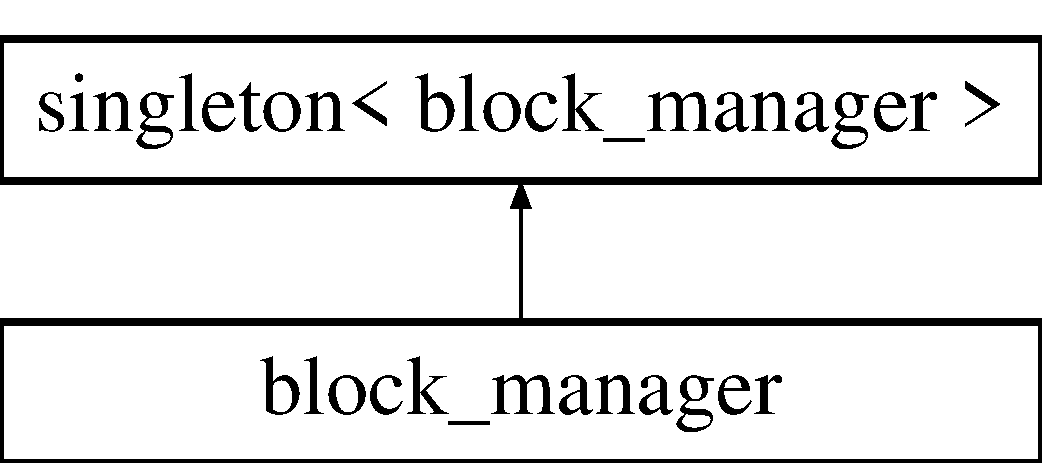
\includegraphics[height=2cm]{classblock__manager}
\end{center}
\end{figure}
\subsection*{Public Member Functions}
\begin{CompactItemize}
\item 
\hypertarget{group__mnglayer_g9d954d295ff1cb73cffd1075e58d6ab5}{
void \textbf{init} (const char $\ast$path, int64\_\-t disk\_\-size=1000 $\ast$1024 $\ast$1024)}
\label{group__mnglayer_g9d954d295ff1cb73cffd1075e58d6ab5}

\item 
{\footnotesize template$<$class BIDIteratorClass $>$ }\\void \hyperlink{group__mnglayer_gb012fd7abe2b4b529b9f6b339aff4232}{new\_\-blocks} (BIDIteratorClass bidbegin, BIDIteratorClass bidend)
\begin{CompactList}\small\item\em Allocates new blocks. \item\end{CompactList}\item 
{\footnotesize template$<$class BlockType , class BIDIteratorClass $>$ }\\void \hyperlink{group__mnglayer_ge77531e60b365f05da213ba7d8b17c9a}{new\_\-blocks} (const unsigned\_\-type nblocks, BIDIteratorClass out)
\item 
{\footnotesize template$<$class BIDIteratorClass $>$ }\\void \hyperlink{group__mnglayer_g0a41492a2faef107fb3c5a7c1ce5ee2d}{delete\_\-blocks} (const BIDIteratorClass \&bidbegin, const BIDIteratorClass \&bidend)
\begin{CompactList}\small\item\em Deallocates blocks. \item\end{CompactList}\item 
{\footnotesize template$<$unsigned BLK\_\-SIZE$>$ }\\void \hyperlink{group__mnglayer_g021e2ef7f3d56eb6dda56958ff5e0739}{delete\_\-block} (const \hyperlink{structBID}{BID}$<$ BLK\_\-SIZE $>$ \&bid)
\begin{CompactList}\small\item\em Deallocates a block. \item\end{CompactList}\item 
\hypertarget{group__mnglayer_g7f79d73b67f9353279c7da98450bb2da}{
{\footnotesize template$<$class BIDType , class OutputIterator $>$ }\\void \textbf{new\_\-blocks\_\-int} (const unsigned\_\-type nblocks, OutputIterator out)}
\label{group__mnglayer_g7f79d73b67f9353279c7da98450bb2da}

\item 
\hypertarget{group__mnglayer_gb141f255591ea232174c110922490f3b}{
{\footnotesize template$<$class BlockType , class OutputIterator $>$ }\\void \textbf{new\_\-blocks} (const unsigned\_\-type nblocks, OutputIterator out)}
\label{group__mnglayer_gb141f255591ea232174c110922490f3b}

\end{CompactItemize}
\subsection*{Protected Member Functions}
\begin{CompactItemize}
\item 
\hypertarget{group__mnglayer_g36a3a4625156d5b9d17b91ce7e1e1874}{
{\footnotesize template$<$class BIDType , class BIDIteratorClass $>$ }\\void \textbf{new\_\-blocks\_\-int} (const unsigned\_\-type nblocks, BIDIteratorClass out)}
\label{group__mnglayer_g36a3a4625156d5b9d17b91ce7e1e1874}

\end{CompactItemize}
\subsection*{Friends}
\begin{CompactItemize}
\item 
\hypertarget{classblock__manager_00478610313143f139a21c4b7b4f1093}{
class \textbf{singleton$<$ block\_\-manager $>$}}
\label{classblock__manager_00478610313143f139a21c4b7b4f1093}

\end{CompactItemize}


\subsection{Detailed Description}
Block manager class. 

Manages allocation and deallocation of blocks in multiple/single disk setting \begin{Desc}
\item[Remarks:]is a singleton \end{Desc}


Definition at line 718 of file main.h.

The documentation for this class was generated from the following file:\begin{CompactItemize}
\item 
/home/Kevin/izenelib/include/am/blockmanager/main.h\end{CompactItemize}

\hypertarget{classblock__w__bids}{
\section{block\_\-w\_\-bids$<$ T, Size\_\-, RawSize\_\-, NBids\_\- $>$ Class Template Reference}
\label{classblock__w__bids}\index{block\_\-w\_\-bids@{block\_\-w\_\-bids}}
}
Contains \hyperlink{structBID}{BID} references for {\tt \hyperlink{classtyped__block}{typed\_\-block}} , not intended for direct use.  


{\tt \#include $<$main.h$>$}

Inheritance diagram for block\_\-w\_\-bids$<$ T, Size\_\-, RawSize\_\-, NBids\_\- $>$::\begin{figure}[H]
\begin{center}
\leavevmode
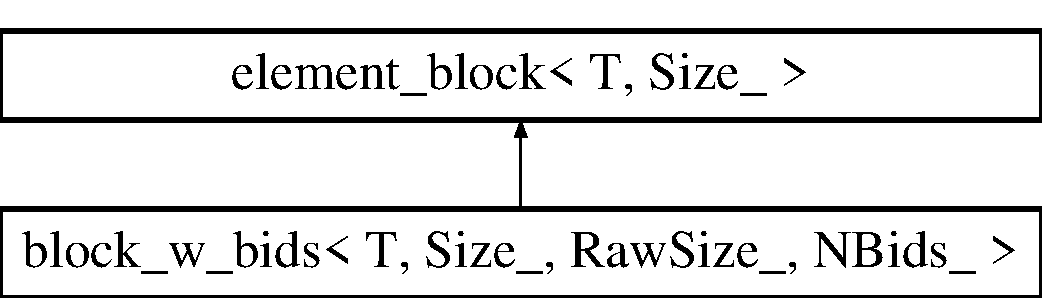
\includegraphics[height=2cm]{classblock__w__bids}
\end{center}
\end{figure}
\subsection*{Public Types}
\begin{CompactItemize}
\item 
enum \{ \textbf{raw\_\-size} =  RawSize\_\-, 
\textbf{nbids} =  NBids\_\-
 \}
\item 
\hypertarget{group__mnglayer_g3418b30447bfa7129dabe6682e1df1a7}{
typedef \hyperlink{structBID}{BID}$<$ raw\_\-size $>$ \textbf{bid\_\-type}}
\label{group__mnglayer_g3418b30447bfa7129dabe6682e1df1a7}

\end{CompactItemize}
\subsection*{Public Member Functions}
\begin{CompactItemize}
\item 
\hypertarget{group__mnglayer_gf8ec031f551ea91964414679972173fd}{
\hyperlink{structBID}{bid\_\-type} \& \hyperlink{group__mnglayer_gf8ec031f551ea91964414679972173fd}{operator()} (int i)}
\label{group__mnglayer_gf8ec031f551ea91964414679972173fd}

\begin{CompactList}\small\item\em An operator to access bid references. \item\end{CompactList}\end{CompactItemize}
\subsection*{Public Attributes}
\begin{CompactItemize}
\item 
\hypertarget{group__mnglayer_g4809f5f95e04ae33cec5ea5a5edd5db3}{
\hyperlink{structBID}{bid\_\-type} \hyperlink{group__mnglayer_g4809f5f95e04ae33cec5ea5a5edd5db3}{ref} \mbox{[}nbids\mbox{]}}
\label{group__mnglayer_g4809f5f95e04ae33cec5ea5a5edd5db3}

\begin{CompactList}\small\item\em Array of \hyperlink{structBID}{BID} references. \item\end{CompactList}\end{CompactItemize}


\subsection{Detailed Description}
\subsubsection*{template$<$class T, unsigned Size\_\-, unsigned RawSize\_\-, unsigned NBids\_\- = 0$>$ class block\_\-w\_\-bids$<$ T, Size\_\-, RawSize\_\-, NBids\_\- $>$}

Contains \hyperlink{structBID}{BID} references for {\tt \hyperlink{classtyped__block}{typed\_\-block}} , not intended for direct use. 

Definition at line 188 of file main.h.

The documentation for this class was generated from the following file:\begin{CompactItemize}
\item 
/home/Kevin/izenelib/include/am/blockmanager/main.h\end{CompactItemize}

\hypertarget{classblock__w__info}{
\section{block\_\-w\_\-info$<$ T\_\-, RawSize\_\-, NBids\_\-, InfoType\_\- $>$ Class Template Reference}
\label{classblock__w__info}\index{block\_\-w\_\-info@{block\_\-w\_\-info}}
}
Contains per block information for {\tt \hyperlink{classtyped__block}{typed\_\-block}} , not intended for direct use.  


{\tt \#include $<$main.h$>$}

Inheritance diagram for block\_\-w\_\-info$<$ T\_\-, RawSize\_\-, NBids\_\-, InfoType\_\- $>$::\begin{figure}[H]
\begin{center}
\leavevmode
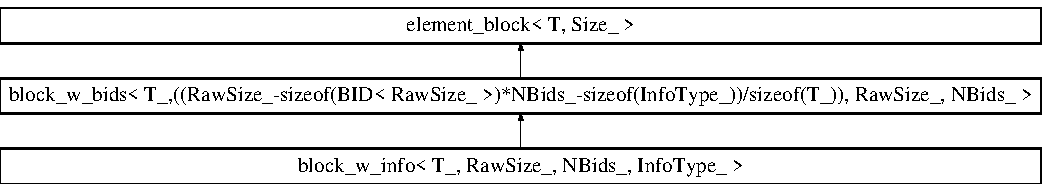
\includegraphics[height=2.47423cm]{classblock__w__info}
\end{center}
\end{figure}
\subsection*{Public Types}
\begin{CompactItemize}
\item 
enum \{ \hyperlink{group__mnglayer_gg64e9c147e936f85096c89f816d71695c79551ce6ebb37de68c336bcae6d9c201}{size} =  ((RawSize\_\- - sizeof(BID$<$RawSize\_\-$>$) $\ast$ NBids\_\- - sizeof(InfoType\_\-)) / sizeof(T\_\-))
 \}
\item 
\hypertarget{classblock__w__info_c3678c48b0e137d29be1c0b1fb40d120}{
typedef InfoType\_\- \hyperlink{classblock__w__info_c3678c48b0e137d29be1c0b1fb40d120}{info\_\-type}}
\label{classblock__w__info_c3678c48b0e137d29be1c0b1fb40d120}

\begin{CompactList}\small\item\em Type of per block information element. \item\end{CompactList}\end{CompactItemize}
\subsection*{Public Attributes}
\begin{CompactItemize}
\item 
\hypertarget{group__mnglayer_gbd86ea875a9e866a9c9d7c9d66dc16d0}{
\hyperlink{classblock__w__info_c3678c48b0e137d29be1c0b1fb40d120}{info\_\-type} \hyperlink{group__mnglayer_gbd86ea875a9e866a9c9d7c9d66dc16d0}{info}}
\label{group__mnglayer_gbd86ea875a9e866a9c9d7c9d66dc16d0}

\begin{CompactList}\small\item\em Per block information element. \item\end{CompactList}\end{CompactItemize}


\subsection{Detailed Description}
\subsubsection*{template$<$class T\_\-, unsigned RawSize\_\-, unsigned NBids\_\-, class InfoType\_\- = void$>$ class block\_\-w\_\-info$<$ T\_\-, RawSize\_\-, NBids\_\-, InfoType\_\- $>$}

Contains per block information for {\tt \hyperlink{classtyped__block}{typed\_\-block}} , not intended for direct use. 

Definition at line 226 of file main.h.

The documentation for this class was generated from the following file:\begin{CompactItemize}
\item 
/home/Kevin/izenelib/include/am/blockmanager/main.h\end{CompactItemize}

\hypertarget{classboostfd__request}{
\section{boostfd\_\-request Class Reference}
\label{classboostfd__request}\index{boostfd\_\-request@{boostfd\_\-request}}
}
Implementation based on boost::iostreams::file\_\-decriptor.  


{\tt \#include $<$iobase.h$>$}

Inheritance diagram for boostfd\_\-request::\begin{figure}[H]
\begin{center}
\leavevmode
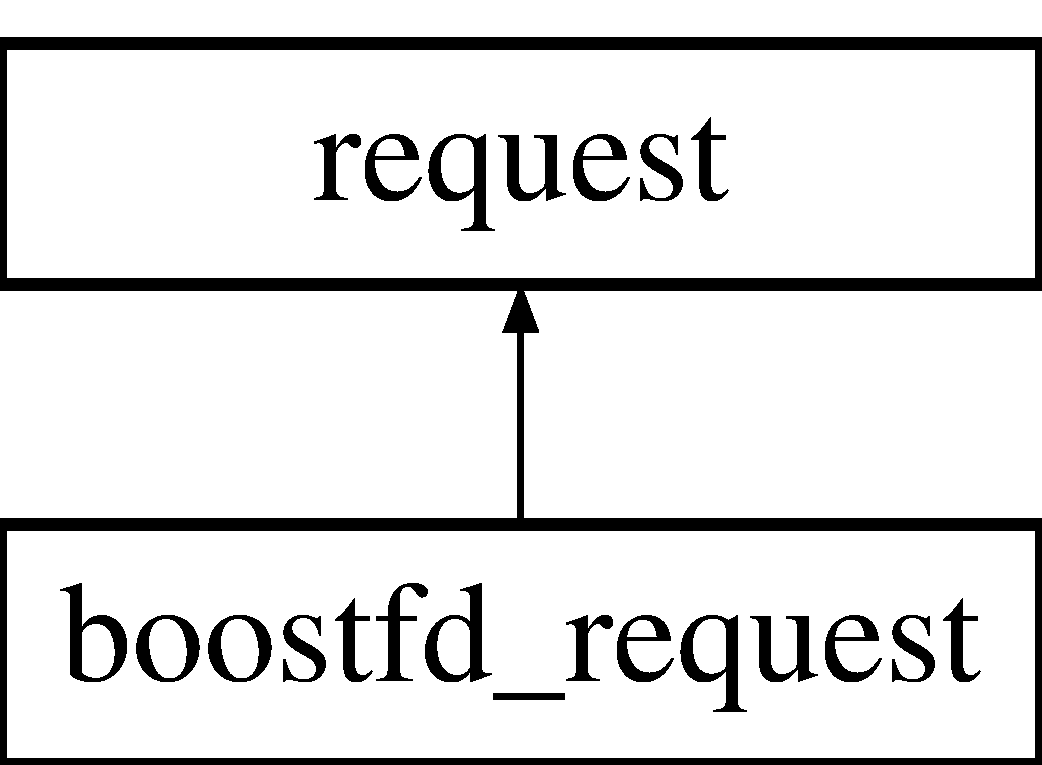
\includegraphics[height=2cm]{classboostfd__request}
\end{center}
\end{figure}
\subsection*{Public Member Functions}
\begin{CompactItemize}
\item 
\hypertarget{group__iolayer_g6e561d1080c80655590c5685f746174f}{
void \hyperlink{group__iolayer_g6e561d1080c80655590c5685f746174f}{wait} ()}
\label{group__iolayer_g6e561d1080c80655590c5685f746174f}

\begin{CompactList}\small\item\em Suspends calling thread until completion of the \hyperlink{classrequest}{request}. \item\end{CompactList}\item 
bool \hyperlink{group__iolayer_g3ec494e77ffa0621380e54cdc4cda657}{poll} ()
\begin{CompactList}\small\item\em Polls the status of the \hyperlink{classrequest}{request}. \item\end{CompactList}\end{CompactItemize}
\subsection*{Protected Types}
\begin{CompactItemize}
\item 
enum \{ \textbf{OP} =  0, 
\textbf{DONE} =  1, 
\textbf{READY2DIE} =  2
 \}
\end{CompactItemize}
\subsection*{Protected Member Functions}
\begin{CompactItemize}
\item 
\hypertarget{group__iolayer_gfa21a04d9716110f605b9739aad2281c}{
\textbf{boostfd\_\-request} (boostfd\_\-file $\ast$f, void $\ast$buf, int64\_\-t off, size\_\-t b, request\_\-type t, \hyperlink{classcompletion__handler}{completion\_\-handler} on\_\-cmpl)}
\label{group__iolayer_gfa21a04d9716110f605b9739aad2281c}

\item 
\hypertarget{group__iolayer_ga8f9033492c4dc7596ef77c56fff15d6}{
bool \textbf{add\_\-waiter} (onoff\_\-switch $\ast$sw)}
\label{group__iolayer_ga8f9033492c4dc7596ef77c56fff15d6}

\item 
\hypertarget{group__iolayer_g1e8576c3e916fbac0ea8c28551c9c4ab}{
void \textbf{delete\_\-waiter} (onoff\_\-switch $\ast$sw)}
\label{group__iolayer_g1e8576c3e916fbac0ea8c28551c9c4ab}

\item 
\hypertarget{group__iolayer_gf0a44abb0c368e4c859eb8abf48a52d2}{
int \textbf{nwaiters} ()}
\label{group__iolayer_gf0a44abb0c368e4c859eb8abf48a52d2}

\item 
\hypertarget{group__iolayer_g91d7f4fb290408511cb6d8c9f5156d87}{
void \textbf{serve} ()}
\label{group__iolayer_g91d7f4fb290408511cb6d8c9f5156d87}

\end{CompactItemize}
\subsection*{Protected Attributes}
\begin{CompactItemize}
\item 
\hypertarget{group__iolayer_g68db8fb13fe5bdb92c44af64db4b8e23}{
state \textbf{\_\-state}}
\label{group__iolayer_g68db8fb13fe5bdb92c44af64db4b8e23}

\item 
\hypertarget{group__iolayer_gc709fb7a7f61caa12ad0036e1d1ee8e8}{
boost::mutex \textbf{waiters\_\-mutex}}
\label{group__iolayer_gc709fb7a7f61caa12ad0036e1d1ee8e8}

\item 
\hypertarget{group__iolayer_g8ea60a2547e82af4ca15f3314a552d2c}{
std::set$<$ onoff\_\-switch $\ast$ $>$ \textbf{waiters}}
\label{group__iolayer_g8ea60a2547e82af4ca15f3314a552d2c}

\end{CompactItemize}
\subsection*{Friends}
\begin{CompactItemize}
\item 
\hypertarget{classboostfd__request_6f659a8c47e4333d9d49f1e05c8d9a45}{
class \textbf{boostfd\_\-file}}
\label{classboostfd__request_6f659a8c47e4333d9d49f1e05c8d9a45}

\end{CompactItemize}


\subsection{Detailed Description}
Implementation based on boost::iostreams::file\_\-decriptor. 

Definition at line 804 of file iobase.h.

The documentation for this class was generated from the following file:\begin{CompactItemize}
\item 
/home/Kevin/izenelib/include/am/blockmanager/iobase.h\end{CompactItemize}

\hypertarget{classBTreeFile}{
\section{BTreeFile$<$ KeyType, ValueType, LockType, Alloc $>$ Class Template Reference}
\label{classBTreeFile}\index{BTreeFile@{BTreeFile}}
}
\hyperlink{classfile}{file} version of B tree.  


{\tt \#include $<$BTreeFile.h$>$}

Inheritance diagram for BTreeFile$<$ KeyType, ValueType, LockType, Alloc $>$::\begin{figure}[H]
\begin{center}
\leavevmode
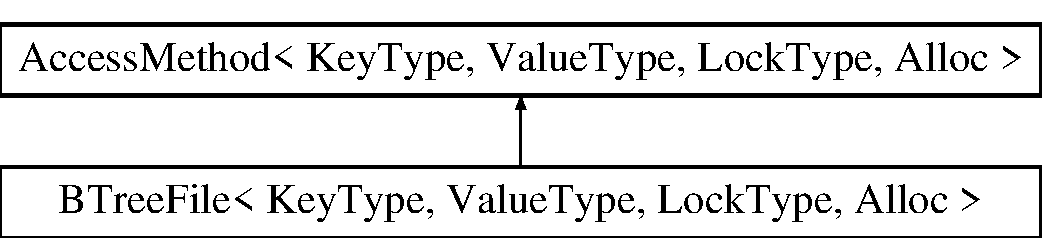
\includegraphics[height=2cm]{classBTreeFile}
\end{center}
\end{figure}
\subsection*{Classes}
\begin{CompactItemize}
\item 
struct \textbf{SFileHeader}
\begin{CompactList}\small\item\em it provides the basical information of the btree. \item\end{CompactList}\end{CompactItemize}
\subsection*{Public Types}
\begin{CompactItemize}
\item 
\hypertarget{classBTreeFile_134b19172aabde32c62243dbdc152a56}{
typedef DataType$<$ KeyType, ValueType $>$ \textbf{DataType}}
\label{classBTreeFile_134b19172aabde32c62243dbdc152a56}

\item 
\hypertarget{classBTreeFile_4e78d31a7e1d1ef621448d762c6d693a}{
typedef intrusive\_\-ptr$<$ BTreeNode$<$ KeyType, DataType, LockType, Alloc $>$ $>$ \textbf{BTreeNodePtr}}
\label{classBTreeFile_4e78d31a7e1d1ef621448d762c6d693a}

\item 
\hypertarget{classBTreeFile_73a488e58ea39521604de5a3df286716}{
typedef std::vector$<$ BTreeNodePtr $>$ \textbf{BTreeNodeVECTOR}}
\label{classBTreeFile_73a488e58ea39521604de5a3df286716}

\item 
\hypertarget{classBTreeFile_ff079237e9726291f48f7429bc97a3ad}{
typedef std::vector$<$ BTreeNodePtr $>$::iterator \textbf{BnPtrIter}}
\label{classBTreeFile_ff079237e9726291f48f7429bc97a3ad}

\item 
\hypertarget{classBTreeFile_c84b666e8b3083625a71371825583863}{
typedef std::pair$<$ BTreeNodePtr, size\_\-t $>$ \textbf{SDBCursor}}
\label{classBTreeFile_c84b666e8b3083625a71371825583863}

\item 
\hypertarget{classBTreeFile_50d1379e8f22b810c4c53c34072db39c}{
typedef intrusive\_\-ptr$<$ PtrObj$<$ DataType, LockType, Alloc $>$ $>$ \textbf{DataTypePtr}}
\label{classBTreeFile_50d1379e8f22b810c4c53c34072db39c}

\item 
\hypertarget{classBTreeFile_ee29e8d1f6bb9700d852eb1fa914491b}{
typedef std::vector$<$ DataTypePtr $>$ \textbf{DataTypeVECTOR}}
\label{classBTreeFile_ee29e8d1f6bb9700d852eb1fa914491b}

\item 
\hypertarget{classBTreeFile_1cefa5c1f36a97524f0be807a7882813}{
typedef std::vector$<$ BTreeNodePtr $>$::iterator \textbf{BIT}}
\label{classBTreeFile_1cefa5c1f36a97524f0be807a7882813}

\item 
\hypertarget{classBTreeFile_8fc5e3e778b95fc3313ab4680c2e895c}{
typedef std::vector$<$ DataTypePtr $>$::iterator \textbf{DIT}}
\label{classBTreeFile_8fc5e3e778b95fc3313ab4680c2e895c}

\end{CompactItemize}
\subsection*{Public Member Functions}
\begin{CompactItemize}
\item 
\hyperlink{classBTreeFile_5609875a43e3c7e70229ac4215aafaff}{BTreeFile} (const std::string \&fileName=\char`\"{}sequentialdb.dat\char`\"{})
\begin{CompactList}\small\item\em constructor \item\end{CompactList}\item 
void \hyperlink{classBTreeFile_76116d6e74ebdd94b641e60466454da5}{setDegree} (int degree)
\item 
void \hyperlink{classBTreeFile_b158c5e0ae96fd9cfb74813f984c1117}{setPageSize} (size\_\-t maxDataSize)
\begin{CompactList}\small\item\em set tha pageSize. \item\end{CompactList}\item 
\hypertarget{classBTreeFile_caec90f215e9695158269c82364d735b}{
void \hyperlink{classBTreeFile_caec90f215e9695158269c82364d735b}{setOverFlowPageSize} (size\_\-t overFlowSize)}
\label{classBTreeFile_caec90f215e9695158269c82364d735b}

\begin{CompactList}\small\item\em set size for overflow page. \item\end{CompactList}\item 
void \hyperlink{classBTreeFile_5a758e56495e400540e2829601e06de7}{setCacheSize} (size\_\-t sz)
\item 
\hypertarget{classBTreeFile_77fbd3babf6b5c990022c23569bb8495}{
std::string \hyperlink{classBTreeFile_77fbd3babf6b5c990022c23569bb8495}{getFileName} () const }
\label{classBTreeFile_77fbd3babf6b5c990022c23569bb8495}

\begin{CompactList}\small\item\em return the \hyperlink{classfile}{file} name of the SequentialDB \item\end{CompactList}\item 
bool \hyperlink{classBTreeFile_dbbf4c18dcccd9f9d231a5d546ff4fe6}{open} ()
\begin{CompactList}\small\item\em open the database. \item\end{CompactList}\item 
bool \hyperlink{classBTreeFile_1602f96ee8ffe4db45f563b7eaef1a17}{close} ()
\begin{CompactList}\small\item\em close the database. \item\end{CompactList}\item 
\hypertarget{classBTreeFile_e0579ea1ac46a4179aa641d61c7ac890}{
bool \hyperlink{classBTreeFile_e0579ea1ac46a4179aa641d61c7ac890}{del} (const KeyType \&key)}
\label{classBTreeFile_e0579ea1ac46a4179aa641d61c7ac890}

\begin{CompactList}\small\item\em del an item from the database \item\end{CompactList}\item 
\hypertarget{classBTreeFile_499c91e3aacf1d7037dcf16321fb8f5f}{
bool \hyperlink{classBTreeFile_499c91e3aacf1d7037dcf16321fb8f5f}{insert} (const DataType \&rec)}
\label{classBTreeFile_499c91e3aacf1d7037dcf16321fb8f5f}

\begin{CompactList}\small\item\em insert an item. \item\end{CompactList}\item 
\hypertarget{classBTreeFile_013fd27ea98d9b7a91a82adebfa81c63}{
bool \hyperlink{classBTreeFile_013fd27ea98d9b7a91a82adebfa81c63}{insert} (const KeyType \&key, const ValueType \&value)}
\label{classBTreeFile_013fd27ea98d9b7a91a82adebfa81c63}

\begin{CompactList}\small\item\em insert an item. \item\end{CompactList}\item 
\hypertarget{classBTreeFile_4ac312ccea4a625f22067e72300bb46d}{
ValueType $\ast$ \hyperlink{classBTreeFile_4ac312ccea4a625f22067e72300bb46d}{find} (const KeyType \&key)}
\label{classBTreeFile_4ac312ccea4a625f22067e72300bb46d}

\begin{CompactList}\small\item\em find an item given a key. \item\end{CompactList}\item 
\hypertarget{classBTreeFile_60b7d0a808434cf7e6133597564068c7}{
bool \textbf{get} (const KeyType \&key, ValueType \&value)}
\label{classBTreeFile_60b7d0a808434cf7e6133597564068c7}

\item 
\hypertarget{classBTreeFile_9ea7b759915249cdc8d4b1ed22f445f9}{
const ValueType $\ast$ \textbf{find} (const KeyType \&key) const }
\label{classBTreeFile_9ea7b759915249cdc8d4b1ed22f445f9}

\item 
\hypertarget{classBTreeFile_c0133f9c22ff22f0bb9c64aded50161d}{
bool \hyperlink{classBTreeFile_c0133f9c22ff22f0bb9c64aded50161d}{update} (const KeyType \&key, const ValueType \&val)}
\label{classBTreeFile_c0133f9c22ff22f0bb9c64aded50161d}

\begin{CompactList}\small\item\em updata an item with given key, if it not exist, insert it directly. \item\end{CompactList}\item 
\hypertarget{classBTreeFile_65845fcc4fd01a769dcf74ac35e233f1}{
bool \hyperlink{classBTreeFile_65845fcc4fd01a769dcf74ac35e233f1}{update} (const DataType \&rec)}
\label{classBTreeFile_65845fcc4fd01a769dcf74ac35e233f1}

\begin{CompactList}\small\item\em updata an item with given key, if it not exist, insert it directly. \item\end{CompactList}\item 
\hypertarget{classBTreeFile_86b258ecee50f2c59e8483750e32aec6}{
int \hyperlink{classBTreeFile_86b258ecee50f2c59e8483750e32aec6}{num\_\-items} ()}
\label{classBTreeFile_86b258ecee50f2c59e8483750e32aec6}

\begin{CompactList}\small\item\em get the number of the items. \item\end{CompactList}\item 
\hypertarget{classBTreeFile_b2ec25ed3809699f44bb5a723e53e94e}{
bool \hyperlink{classBTreeFile_b2ec25ed3809699f44bb5a723e53e94e}{get} (const KeyType \&key, DataType \&rec)}
\label{classBTreeFile_b2ec25ed3809699f44bb5a723e53e94e}

\begin{CompactList}\small\item\em get an item by its key. \item\end{CompactList}\item 
\hypertarget{classBTreeFile_45d39b668e269770ff9402628067a973}{
bool \hyperlink{classBTreeFile_45d39b668e269770ff9402628067a973}{get} (const SDBCursor \&locn, DataType \&rec)}
\label{classBTreeFile_45d39b668e269770ff9402628067a973}

\begin{CompactList}\small\item\em get an item from given Locn. $\ast$ \item\end{CompactList}\item 
\hypertarget{classBTreeFile_1771c662eafbb8d90d945659dcdc9ffd}{
bool \hyperlink{classBTreeFile_1771c662eafbb8d90d945659dcdc9ffd}{get} (const SDBCursor \&locn, KeyType \&key, ValueType \&value)}
\label{classBTreeFile_1771c662eafbb8d90d945659dcdc9ffd}

\begin{CompactList}\small\item\em get an item from given Locn. $\ast$ \item\end{CompactList}\item 
\hypertarget{classBTreeFile_b375e1166dd179b0e6f54c2daff7ae91}{
SDBCursor \hyperlink{classBTreeFile_b375e1166dd179b0e6f54c2daff7ae91}{get\_\-first\_\-locn} ()}
\label{classBTreeFile_b375e1166dd179b0e6f54c2daff7ae91}

\begin{CompactList}\small\item\em get the cursor of the first item. \item\end{CompactList}\item 
\hypertarget{classBTreeFile_dbd89f1e470008e7a008b22a99c9e0b5}{
bool \hyperlink{classBTreeFile_dbd89f1e470008e7a008b22a99c9e0b5}{seq} (SDBCursor \&locn, DataType \&rec, ESeqDirection sdir=ESD\_\-FORWARD)}
\label{classBTreeFile_dbd89f1e470008e7a008b22a99c9e0b5}

\begin{CompactList}\small\item\em get the next or prev item. \item\end{CompactList}\item 
\hypertarget{classBTreeFile_0fb8cd6989e717ddefcd9514657c708b}{
KeyType \hyperlink{classBTreeFile_0fb8cd6989e717ddefcd9514657c708b}{getNext} (const KeyType \&key)}
\label{classBTreeFile_0fb8cd6989e717ddefcd9514657c708b}

\begin{CompactList}\small\item\em given a key, get next key \item\end{CompactList}\item 
\hypertarget{classBTreeFile_5b2991be9d5c88ae1b269572e6ee2747}{
KeyType \hyperlink{classBTreeFile_5b2991be9d5c88ae1b269572e6ee2747}{getPrev} (const KeyType \&key)}
\label{classBTreeFile_5b2991be9d5c88ae1b269572e6ee2747}

\begin{CompactList}\small\item\em given a key, get next key \item\end{CompactList}\item 
\hypertarget{classBTreeFile_23afa194f796512b34c002af01dc25a8}{
void \hyperlink{classBTreeFile_23afa194f796512b34c002af01dc25a8}{flush} ()}
\label{classBTreeFile_23afa194f796512b34c002af01dc25a8}

\begin{CompactList}\small\item\em write all the items in memory to \hyperlink{classfile}{file}. \item\end{CompactList}\item 
\hypertarget{classBTreeFile_3efffc668457bd1d85a08bef461731b9}{
void \hyperlink{classBTreeFile_3efffc668457bd1d85a08bef461731b9}{commit} ()}
\label{classBTreeFile_3efffc668457bd1d85a08bef461731b9}

\begin{CompactList}\small\item\em write back the dirypages \item\end{CompactList}\item 
void \hyperlink{classBTreeFile_005fb40d2dbb29e75ef0a0a7a4faa71d}{display} (std::ostream \&os=std::cout, bool onlyheader=true)
\item 
KeyType \hyperlink{classBTreeFile_05829fd2f39c24fe36b5a3a395437de9}{getNearest} (const KeyType \&key)
\item 
\hypertarget{classBTreeFile_8fca5f21802218f0a654e1c70e51d193}{
SDBCursor \hyperlink{classBTreeFile_8fca5f21802218f0a654e1c70e51d193}{search} (const KeyType \&key)}
\label{classBTreeFile_8fca5f21802218f0a654e1c70e51d193}

\begin{CompactList}\small\item\em External method that searches for elements that match the given key. \item\end{CompactList}\item 
\hypertarget{classBTreeFile_f175ce31694ff970ef09e90a29358770}{
bool \textbf{search} (const KeyType \&key, SDBCursor \&locn)}
\label{classBTreeFile_f175ce31694ff970ef09e90a29358770}

\end{CompactItemize}


\subsection{Detailed Description}
\subsubsection*{template$<$typename KeyType, typename ValueType = NullType, typename LockType = NullLock, typename Alloc = std::allocator$<$DataType$<$KeyType,ValueType$>$ $>$$>$ class BTreeFile$<$ KeyType, ValueType, LockType, Alloc $>$}

\hyperlink{classfile}{file} version of B tree. 

$|$----------------$|$ $|$ magic $|$ $|$----------------$|$ $|$ minDegree $|$ /then the order of the btree is 2$\ast$minDegree-1. $|$----------------$|$ $|$ pageSize $|$ $|$----------------$|$ $|$ cacheSize $|$ $|$----------------$|$ $|$ ..... $|$ $|$----------------$|$ $|$ numItem $|$ $|$----------------$|$ $|$ rootPos $|$ $|$----------------$|$ 

Definition at line 46 of file BTreeFile.h.

\subsection{Constructor \& Destructor Documentation}
\hypertarget{classBTreeFile_5609875a43e3c7e70229ac4215aafaff}{
\index{BTreeFile@{BTreeFile}!BTreeFile@{BTreeFile}}
\index{BTreeFile@{BTreeFile}!BTreeFile@{BTreeFile}}
\subsubsection[{BTreeFile}]{\setlength{\rightskip}{0pt plus 5cm}template$<$typename KeyType , typename ValueType , typename LockType , typename Alloc $>$ {\bf BTreeFile}$<$ KeyType, ValueType, LockType, Alloc $>$::{\bf BTreeFile} (const std::string \& {\em fileName} = {\tt \char`\"{}sequentialdb.dat\char`\"{}})\hspace{0.3cm}{\tt  \mbox{[}inline\mbox{]}}}}
\label{classBTreeFile_5609875a43e3c7e70229ac4215aafaff}


constructor 

\begin{Desc}
\item[Parameters:]
\begin{description}
\item[{\em minDegree,default}]is 2, i.e the order is 3. \end{description}
\end{Desc}


Definition at line 714 of file BTreeFile.h.

\subsection{Member Function Documentation}
\hypertarget{classBTreeFile_1602f96ee8ffe4db45f563b7eaef1a17}{
\index{BTreeFile@{BTreeFile}!close@{close}}
\index{close@{close}!BTreeFile@{BTreeFile}}
\subsubsection[{close}]{\setlength{\rightskip}{0pt plus 5cm}template$<$typename KeyType , typename ValueType  = NullType, typename LockType  = NullLock, typename Alloc  = std::allocator$<$DataType$<$KeyType,ValueType$>$ $>$$>$ bool {\bf BTreeFile}$<$ KeyType, ValueType, LockType, Alloc $>$::close ()\hspace{0.3cm}{\tt  \mbox{[}inline\mbox{]}}}}
\label{classBTreeFile_1602f96ee8ffe4db45f563b7eaef1a17}


close the database. 

if we don't call it, it will be automately called in deconstructor 

Definition at line 131 of file BTreeFile.h.\hypertarget{classBTreeFile_005fb40d2dbb29e75ef0a0a7a4faa71d}{
\index{BTreeFile@{BTreeFile}!display@{display}}
\index{display@{display}!BTreeFile@{BTreeFile}}
\subsubsection[{display}]{\setlength{\rightskip}{0pt plus 5cm}template$<$typename KeyType , typename ValueType  = NullType, typename LockType  = NullLock, typename Alloc  = std::allocator$<$DataType$<$KeyType,ValueType$>$ $>$$>$ void {\bf BTreeFile}$<$ KeyType, ValueType, LockType, Alloc $>$::display (std::ostream \& {\em os} = {\tt std::cout}, \/  bool {\em onlyheader} = {\tt true})\hspace{0.3cm}{\tt  \mbox{[}inline\mbox{]}}}}
\label{classBTreeFile_005fb40d2dbb29e75ef0a0a7a4faa71d}


for debug. print the shape of the B tree. 

Definition at line 320 of file BTreeFile.h.\hypertarget{classBTreeFile_05829fd2f39c24fe36b5a3a395437de9}{
\index{BTreeFile@{BTreeFile}!getNearest@{getNearest}}
\index{getNearest@{getNearest}!BTreeFile@{BTreeFile}}
\subsubsection[{getNearest}]{\setlength{\rightskip}{0pt plus 5cm}template$<$typename KeyType , typename ValueType  = NullType, typename LockType  = NullLock, typename Alloc  = std::allocator$<$DataType$<$KeyType,ValueType$>$ $>$$>$ KeyType {\bf BTreeFile}$<$ KeyType, ValueType, LockType, Alloc $>$::getNearest (const KeyType \& {\em key})\hspace{0.3cm}{\tt  \mbox{[}inline\mbox{]}}}}
\label{classBTreeFile_05829fd2f39c24fe36b5a3a395437de9}


if the input key exists, just return itself, otherwise return the smallest existing key that bigger than it. 

Definition at line 329 of file BTreeFile.h.\hypertarget{classBTreeFile_dbbf4c18dcccd9f9d231a5d546ff4fe6}{
\index{BTreeFile@{BTreeFile}!open@{open}}
\index{open@{open}!BTreeFile@{BTreeFile}}
\subsubsection[{open}]{\setlength{\rightskip}{0pt plus 5cm}template$<$typename KeyType , typename ValueType , typename LockType , typename Alloc $>$ bool {\bf BTreeFile}$<$ KeyType, ValueType, LockType, Alloc $>$::open ()\hspace{0.3cm}{\tt  \mbox{[}inline\mbox{]}}}}
\label{classBTreeFile_dbbf4c18dcccd9f9d231a5d546ff4fe6}


open the database. 

Everytime we use the database, we mush open it first. 

Definition at line 1178 of file BTreeFile.h.\hypertarget{classBTreeFile_5a758e56495e400540e2829601e06de7}{
\index{BTreeFile@{BTreeFile}!setCacheSize@{setCacheSize}}
\index{setCacheSize@{setCacheSize}!BTreeFile@{BTreeFile}}
\subsubsection[{setCacheSize}]{\setlength{\rightskip}{0pt plus 5cm}template$<$typename KeyType , typename ValueType  = NullType, typename LockType  = NullLock, typename Alloc  = std::allocator$<$DataType$<$KeyType,ValueType$>$ $>$$>$ void {\bf BTreeFile}$<$ KeyType, ValueType, LockType, Alloc $>$::setCacheSize (size\_\-t {\em sz})\hspace{0.3cm}{\tt  \mbox{[}inline\mbox{]}}}}
\label{classBTreeFile_5a758e56495e400540e2829601e06de7}


We would peroidically flush the memory items, according to the cache Size. 

Definition at line 108 of file BTreeFile.h.\hypertarget{classBTreeFile_76116d6e74ebdd94b641e60466454da5}{
\index{BTreeFile@{BTreeFile}!setDegree@{setDegree}}
\index{setDegree@{setDegree}!BTreeFile@{BTreeFile}}
\subsubsection[{setDegree}]{\setlength{\rightskip}{0pt plus 5cm}template$<$typename KeyType , typename ValueType  = NullType, typename LockType  = NullLock, typename Alloc  = std::allocator$<$DataType$<$KeyType,ValueType$>$ $>$$>$ void {\bf BTreeFile}$<$ KeyType, ValueType, LockType, Alloc $>$::setDegree (int {\em degree})\hspace{0.3cm}{\tt  \mbox{[}inline\mbox{]}}}}
\label{classBTreeFile_76116d6e74ebdd94b641e60466454da5}


set the degree 

Definition at line 71 of file BTreeFile.h.\hypertarget{classBTreeFile_b158c5e0ae96fd9cfb74813f984c1117}{
\index{BTreeFile@{BTreeFile}!setPageSize@{setPageSize}}
\index{setPageSize@{setPageSize}!BTreeFile@{BTreeFile}}
\subsubsection[{setPageSize}]{\setlength{\rightskip}{0pt plus 5cm}template$<$typename KeyType , typename ValueType  = NullType, typename LockType  = NullLock, typename Alloc  = std::allocator$<$DataType$<$KeyType,ValueType$>$ $>$$>$ void {\bf BTreeFile}$<$ KeyType, ValueType, LockType, Alloc $>$::setPageSize (size\_\-t {\em maxDataSize})\hspace{0.3cm}{\tt  \mbox{[}inline\mbox{]}}}}
\label{classBTreeFile_b158c5e0ae96fd9cfb74813f984c1117}


set tha pageSize. 

\begin{Desc}
\item[Parameters:]
\begin{description}
\item[{\em maxDataSize}]if the size of DataType(binary) exceeds maxDataSize, overflowing accur. if we can predict it first, we can reduce the \hyperlink{classfile}{file} space. \end{description}
\end{Desc}


Definition at line 81 of file BTreeFile.h.

The documentation for this class was generated from the following file:\begin{CompactItemize}
\item 
/home/Kevin/izenelib/include/am/btree/BTreeFile.h\end{CompactItemize}

\hypertarget{classBTrie}{
\section{BTrie$<$ STRING\_\-TYPE, ALPHABET, ALPHABET\_\-SIZE, BUCKET\_\-SIZE, SPLIT\_\-RATIO, ENTRY\_\-SIZE\_\-POW, HASH\_\-FUNCTION, INIT\_\-BUCKET\_\-SIZE, BUCKET\_\-CACHE\_\-LENGTH, BucketCachePolicy, NODE\_\-CACHE\_\-LENGTH, NodeCachePolicy $>$ Class Template Reference}
\label{classBTrie}\index{BTrie@{BTrie}}
}
{\tt \#include $<$b\_\-trie.hpp$>$}

\subsection*{Public Member Functions}
\begin{CompactItemize}
\item 
\hyperlink{classBTrie_3cc0735f4735169d28c2fdc3c052ad7f}{BTrie} (const string \&filename=\char`\"{}\_\-btrie\char`\"{})
\item 
void \hyperlink{classBTrie_bfa4a5883b5b6146af18c53a35e85b34}{flush} ()
\item 
void \hyperlink{classBTrie_8808c1f6c8b72d7b72b70646ec661837}{load} ()
\item 
bool \hyperlink{classBTrie_7cec73d8ae32a6d049f3e801f6ee75f3}{insert} (const STRING\_\-TYPE \&str, uint64\_\-t contentAddr)
\item 
void \hyperlink{classBTrie_3e3f5765235c78ab56663a0852c1178d}{splitBucket} (BucketPtr \&b, AlphabetNodePtr \&n, uint64\_\-t diskAddr, uint32\_\-t idx, vector$<$ STRING\_\-TYPE $>$ \&leftStr, vector$<$ uint64\_\-t $>$ \&leftAddr)
\item 
bool \hyperlink{classBTrie_8f000cc39b2de657cd7817690437f54d}{del} (const STRING\_\-TYPE \&str)
\item 
bool \hyperlink{classBTrie_7557a9c4d0eb728ca0bcbd417d922f17}{update} (const STRING\_\-TYPE \&str, uint64\_\-t contentAddr)
\item 
\hypertarget{classBTrie_b9b758f3217a31d8e66dede82b742cda}{
bool \textbf{findRegExp} (const STRING\_\-TYPE \&regexp, vector$<$ uint32\_\-t $>$ \&ret)}
\label{classBTrie_b9b758f3217a31d8e66dede82b742cda}

\item 
\hypertarget{classBTrie_ed05bb9612951db278a752c8a9818ba5}{
bool \textbf{findRegExp} (const STRING\_\-TYPE \&regexp, vector$<$ item\_\-pair$<$ STRING\_\-TYPE $>$ $>$ \&ret)}
\label{classBTrie_ed05bb9612951db278a752c8a9818ba5}

\item 
uint64\_\-t \hyperlink{classBTrie_3c466397db53b56baa0def869f49a1f3}{find} (const STRING\_\-TYPE \&str)
\item 
uint32\_\-t \hyperlink{classBTrie_71cd037bb6ec881966cc91264377e35e}{getNodeAmount} () const 
\item 
\hypertarget{classBTrie_a31346d8cf5b9ffbf00873b726cb04db}{
void \textbf{display} (ostream \&os, const STRING\_\-TYPE \&str)}
\label{classBTrie_a31346d8cf5b9ffbf00873b726cb04db}

\item 
\hypertarget{classBTrie_6004a5f648926b28e5cd4820756aae45}{
BucketPtr \textbf{loadBucket} (uint32\_\-t \&memAddr, uint64\_\-t diskAddr)}
\label{classBTrie_6004a5f648926b28e5cd4820756aae45}

\item 
\hypertarget{classBTrie_67416e8012c149630658da525533b0c2}{
BucketPtr \textbf{newBucket} ()}
\label{classBTrie_67416e8012c149630658da525533b0c2}

\end{CompactItemize}
\subsection*{Protected Member Functions}
\begin{CompactItemize}
\item 
\hypertarget{classBTrie_8a979fa156b124ba6fa442cc1190ad35}{
void \textbf{load\_\-} (AlphabetNodePtr \&n)}
\label{classBTrie_8a979fa156b124ba6fa442cc1190ad35}

\item 
\hypertarget{classBTrie_d518bfc4264e615479c9afcf0d313954}{
string \textbf{substr} (const string \&str, size\_\-t pos, size\_\-t len=(size\_\-t)-1)}
\label{classBTrie_d518bfc4264e615479c9afcf0d313954}

\item 
\hypertarget{classBTrie_ca2c65640ed76ddd91025bd86b832f97}{
wiselib::UString \textbf{substr} (const wiselib::UString \&str, size\_\-t pos, size\_\-t len=(size\_\-t)-1)}
\label{classBTrie_ca2c65640ed76ddd91025bd86b832f97}

\item 
void \hyperlink{classBTrie_3125cac8b6ba87306a3636bddd0da0f3}{findRegExp\_\-} (uint32\_\-t idx, uint64\_\-t addr, const STRING\_\-TYPE \&regexp, const STRING\_\-TYPE \&sofar, vector$<$ item\_\-pair$<$ STRING\_\-TYPE $>$ $>$ \&ret)
\end{CompactItemize}
\subsection*{Protected Attributes}
\begin{CompactItemize}
\item 
\hypertarget{classBTrie_282779241215a40bd6f64c26c4bb6b67}{
FILE $\ast$ \hyperlink{classBTrie_282779241215a40bd6f64c26c4bb6b67}{nodf\_\-}}
\label{classBTrie_282779241215a40bd6f64c26c4bb6b67}

\begin{CompactList}\small\item\em Node data \hyperlink{classfile}{file} handler. \item\end{CompactList}\item 
\hypertarget{classBTrie_790e90901c61010abf817786d0a72af2}{
FILE $\ast$ \hyperlink{classBTrie_790e90901c61010abf817786d0a72af2}{bukf\_\-}}
\label{classBTrie_790e90901c61010abf817786d0a72af2}

\begin{CompactList}\small\item\em \hyperlink{classBucket}{Bucket} data \hyperlink{classfile}{file} handler. \item\end{CompactList}\item 
\hypertarget{classBTrie_121b3b835910ac94754c123e38b9c982}{
string \hyperlink{classBTrie_121b3b835910ac94754c123e38b9c982}{hashf\_\-}}
\label{classBTrie_121b3b835910ac94754c123e38b9c982}

\begin{CompactList}\small\item\em Hash table data \hyperlink{classfile}{file} handler. \item\end{CompactList}\item 
\hypertarget{classBTrie_60b3acb7798110d53ec589d6929ab1ae}{
BucketCacheType $\ast$ \hyperlink{classBTrie_60b3acb7798110d53ec589d6929ab1ae}{pBucketCache\_\-}}
\label{classBTrie_60b3acb7798110d53ec589d6929ab1ae}

\begin{CompactList}\small\item\em \hyperlink{classBucket}{Bucket} cache. \item\end{CompactList}\item 
\hypertarget{classBTrie_a24075704dcb542c7edec0f6b8d7f008}{
NodeCacheType $\ast$ \hyperlink{classBTrie_a24075704dcb542c7edec0f6b8d7f008}{pNodeCache\_\-}}
\label{classBTrie_a24075704dcb542c7edec0f6b8d7f008}

\begin{CompactList}\small\item\em Nodes cache. \item\end{CompactList}\item 
\hypertarget{classBTrie_99d0b0d47787e8b38e610f096d51e054}{
\hyperlink{classMap}{HashMap} \hyperlink{classBTrie_99d0b0d47787e8b38e610f096d51e054}{hashTable\_\-}}
\label{classBTrie_99d0b0d47787e8b38e610f096d51e054}

\begin{CompactList}\small\item\em Hash table. \item\end{CompactList}\end{CompactItemize}


\subsection{Detailed Description}
\subsubsection*{template$<$class STRING\_\-TYPE = string, typename STRING\_\-TYPE::value\_\-type $\ast$ ALPHABET = a2z, uint32\_\-t ALPHABET\_\-SIZE = a2z\_\-size, uint32\_\-t BUCKET\_\-SIZE = 8196, uint8\_\-t SPLIT\_\-RATIO = 75, size\_\-t ENTRY\_\-SIZE\_\-POW = 10, class HASH\_\-FUNCTION = simple\_\-hash, int INIT\_\-BUCKET\_\-SIZE = 64, uint64\_\-t BUCKET\_\-CACHE\_\-LENGTH = 10000000000, class BucketCachePolicy = CachePolicyLARU, uint64\_\-t NODE\_\-CACHE\_\-LENGTH = 1000000000, class NodeCachePolicy = CachePolicyLARU$>$ class BTrie$<$ STRING\_\-TYPE, ALPHABET, ALPHABET\_\-SIZE, BUCKET\_\-SIZE, SPLIT\_\-RATIO, ENTRY\_\-SIZE\_\-POW, HASH\_\-FUNCTION, INIT\_\-BUCKET\_\-SIZE, BUCKET\_\-CACHE\_\-LENGTH, BucketCachePolicy, NODE\_\-CACHE\_\-LENGTH, NodeCachePolicy $>$}

B-trie is a kind of multi-way tree. There’re two kinds of nodes in that tree. One is normal node which is an alphabet with pointer actually. We just call them ’Node’. The other is called bucket which stores bunches of strings suffix. The prefix is consumed by nodes. And, I store nodes and bucket in 2 different separate files. The insertion of a strings may involve splitting bucket. 

Definition at line 54 of file b\_\-trie.hpp.

\subsection{Constructor \& Destructor Documentation}
\hypertarget{classBTrie_3cc0735f4735169d28c2fdc3c052ad7f}{
\index{BTrie@{BTrie}!BTrie@{BTrie}}
\index{BTrie@{BTrie}!BTrie@{BTrie}}
\subsubsection[{BTrie}]{\setlength{\rightskip}{0pt plus 5cm}template$<$class STRING\_\-TYPE  = string, typename STRING\_\-TYPE::value\_\-type $\ast$ ALPHABET = a2z, uint32\_\-t ALPHABET\_\-SIZE = a2z\_\-size, uint32\_\-t BUCKET\_\-SIZE = 8196, uint8\_\-t SPLIT\_\-RATIO = 75, size\_\-t ENTRY\_\-SIZE\_\-POW = 10, class HASH\_\-FUNCTION  = simple\_\-hash, int INIT\_\-BUCKET\_\-SIZE = 64, uint64\_\-t BUCKET\_\-CACHE\_\-LENGTH = 10000000000, class BucketCachePolicy  = CachePolicyLARU, uint64\_\-t NODE\_\-CACHE\_\-LENGTH = 1000000000, class NodeCachePolicy  = CachePolicyLARU$>$ {\bf BTrie}$<$ STRING\_\-TYPE, ALPHABET, ALPHABET\_\-SIZE, BUCKET\_\-SIZE, SPLIT\_\-RATIO, ENTRY\_\-SIZE\_\-POW, HASH\_\-FUNCTION, INIT\_\-BUCKET\_\-SIZE, BUCKET\_\-CACHE\_\-LENGTH, BucketCachePolicy, NODE\_\-CACHE\_\-LENGTH, NodeCachePolicy $>$::{\bf BTrie} (const string \& {\em filename} = {\tt \char`\"{}\_\-btrie\char`\"{}})\hspace{0.3cm}{\tt  \mbox{[}inline\mbox{]}}}}
\label{classBTrie_3cc0735f4735169d28c2fdc3c052ad7f}


\begin{Desc}
\item[Parameters:]
\begin{description}
\item[{\em filename}]Name of \hyperlink{classfile}{file} stores trie data. It will generate 3 files. The suffix of them are '.buk', '.nod', '.has'. They stands for bucket \hyperlink{classfile}{file}, trie node \hyperlink{classfile}{file} and hash table \hyperlink{classfile}{file} respectively. \end{description}
\end{Desc}


Definition at line 69 of file b\_\-trie.hpp.

\subsection{Member Function Documentation}
\hypertarget{classBTrie_8f000cc39b2de657cd7817690437f54d}{
\index{BTrie@{BTrie}!del@{del}}
\index{del@{del}!BTrie@{BTrie}}
\subsubsection[{del}]{\setlength{\rightskip}{0pt plus 5cm}template$<$class STRING\_\-TYPE  = string, typename STRING\_\-TYPE::value\_\-type $\ast$ ALPHABET = a2z, uint32\_\-t ALPHABET\_\-SIZE = a2z\_\-size, uint32\_\-t BUCKET\_\-SIZE = 8196, uint8\_\-t SPLIT\_\-RATIO = 75, size\_\-t ENTRY\_\-SIZE\_\-POW = 10, class HASH\_\-FUNCTION  = simple\_\-hash, int INIT\_\-BUCKET\_\-SIZE = 64, uint64\_\-t BUCKET\_\-CACHE\_\-LENGTH = 10000000000, class BucketCachePolicy  = CachePolicyLARU, uint64\_\-t NODE\_\-CACHE\_\-LENGTH = 1000000000, class NodeCachePolicy  = CachePolicyLARU$>$ bool {\bf BTrie}$<$ STRING\_\-TYPE, ALPHABET, ALPHABET\_\-SIZE, BUCKET\_\-SIZE, SPLIT\_\-RATIO, ENTRY\_\-SIZE\_\-POW, HASH\_\-FUNCTION, INIT\_\-BUCKET\_\-SIZE, BUCKET\_\-CACHE\_\-LENGTH, BucketCachePolicy, NODE\_\-CACHE\_\-LENGTH, NodeCachePolicy $>$::del (const STRING\_\-TYPE \& {\em str})\hspace{0.3cm}{\tt  \mbox{[}inline\mbox{]}}}}
\label{classBTrie_8f000cc39b2de657cd7817690437f54d}


Delete string in trie. 

Definition at line 449 of file b\_\-trie.hpp.\hypertarget{classBTrie_3c466397db53b56baa0def869f49a1f3}{
\index{BTrie@{BTrie}!find@{find}}
\index{find@{find}!BTrie@{BTrie}}
\subsubsection[{find}]{\setlength{\rightskip}{0pt plus 5cm}template$<$class STRING\_\-TYPE  = string, typename STRING\_\-TYPE::value\_\-type $\ast$ ALPHABET = a2z, uint32\_\-t ALPHABET\_\-SIZE = a2z\_\-size, uint32\_\-t BUCKET\_\-SIZE = 8196, uint8\_\-t SPLIT\_\-RATIO = 75, size\_\-t ENTRY\_\-SIZE\_\-POW = 10, class HASH\_\-FUNCTION  = simple\_\-hash, int INIT\_\-BUCKET\_\-SIZE = 64, uint64\_\-t BUCKET\_\-CACHE\_\-LENGTH = 10000000000, class BucketCachePolicy  = CachePolicyLARU, uint64\_\-t NODE\_\-CACHE\_\-LENGTH = 1000000000, class NodeCachePolicy  = CachePolicyLARU$>$ uint64\_\-t {\bf BTrie}$<$ STRING\_\-TYPE, ALPHABET, ALPHABET\_\-SIZE, BUCKET\_\-SIZE, SPLIT\_\-RATIO, ENTRY\_\-SIZE\_\-POW, HASH\_\-FUNCTION, INIT\_\-BUCKET\_\-SIZE, BUCKET\_\-CACHE\_\-LENGTH, BucketCachePolicy, NODE\_\-CACHE\_\-LENGTH, NodeCachePolicy $>$::find (const STRING\_\-TYPE \& {\em str})\hspace{0.3cm}{\tt  \mbox{[}inline\mbox{]}}}}
\label{classBTrie_3c466397db53b56baa0def869f49a1f3}


Get the content of 'str' 

Definition at line 527 of file b\_\-trie.hpp.\hypertarget{classBTrie_3125cac8b6ba87306a3636bddd0da0f3}{
\index{BTrie@{BTrie}!findRegExp\_\-@{findRegExp\_\-}}
\index{findRegExp\_\-@{findRegExp\_\-}!BTrie@{BTrie}}
\subsubsection[{findRegExp\_\-}]{\setlength{\rightskip}{0pt plus 5cm}template$<$class STRING\_\-TYPE  = string, typename STRING\_\-TYPE::value\_\-type $\ast$ ALPHABET = a2z, uint32\_\-t ALPHABET\_\-SIZE = a2z\_\-size, uint32\_\-t BUCKET\_\-SIZE = 8196, uint8\_\-t SPLIT\_\-RATIO = 75, size\_\-t ENTRY\_\-SIZE\_\-POW = 10, class HASH\_\-FUNCTION  = simple\_\-hash, int INIT\_\-BUCKET\_\-SIZE = 64, uint64\_\-t BUCKET\_\-CACHE\_\-LENGTH = 10000000000, class BucketCachePolicy  = CachePolicyLARU, uint64\_\-t NODE\_\-CACHE\_\-LENGTH = 1000000000, class NodeCachePolicy  = CachePolicyLARU$>$ void {\bf BTrie}$<$ STRING\_\-TYPE, ALPHABET, ALPHABET\_\-SIZE, BUCKET\_\-SIZE, SPLIT\_\-RATIO, ENTRY\_\-SIZE\_\-POW, HASH\_\-FUNCTION, INIT\_\-BUCKET\_\-SIZE, BUCKET\_\-CACHE\_\-LENGTH, BucketCachePolicy, NODE\_\-CACHE\_\-LENGTH, NodeCachePolicy $>$::findRegExp\_\- (uint32\_\-t {\em idx}, \/  uint64\_\-t {\em addr}, \/  const STRING\_\-TYPE \& {\em regexp}, \/  const STRING\_\-TYPE \& {\em sofar}, \/  vector$<$ item\_\-pair$<$ STRING\_\-TYPE $>$ $>$ \& {\em ret})\hspace{0.3cm}{\tt  \mbox{[}inline, protected\mbox{]}}}}
\label{classBTrie_3125cac8b6ba87306a3636bddd0da0f3}


Find regular expression in trie tree. \begin{Desc}
\item[Parameters:]
\begin{description}
\item[{\em regexp}]Regular expression. \item[{\em sofar}]Record the string ahead sofar. \item[{\em ret}]The found results. \end{description}
\end{Desc}


Definition at line 658 of file b\_\-trie.hpp.\hypertarget{classBTrie_bfa4a5883b5b6146af18c53a35e85b34}{
\index{BTrie@{BTrie}!flush@{flush}}
\index{flush@{flush}!BTrie@{BTrie}}
\subsubsection[{flush}]{\setlength{\rightskip}{0pt plus 5cm}template$<$class STRING\_\-TYPE  = string, typename STRING\_\-TYPE::value\_\-type $\ast$ ALPHABET = a2z, uint32\_\-t ALPHABET\_\-SIZE = a2z\_\-size, uint32\_\-t BUCKET\_\-SIZE = 8196, uint8\_\-t SPLIT\_\-RATIO = 75, size\_\-t ENTRY\_\-SIZE\_\-POW = 10, class HASH\_\-FUNCTION  = simple\_\-hash, int INIT\_\-BUCKET\_\-SIZE = 64, uint64\_\-t BUCKET\_\-CACHE\_\-LENGTH = 10000000000, class BucketCachePolicy  = CachePolicyLARU, uint64\_\-t NODE\_\-CACHE\_\-LENGTH = 1000000000, class NodeCachePolicy  = CachePolicyLARU$>$ void {\bf BTrie}$<$ STRING\_\-TYPE, ALPHABET, ALPHABET\_\-SIZE, BUCKET\_\-SIZE, SPLIT\_\-RATIO, ENTRY\_\-SIZE\_\-POW, HASH\_\-FUNCTION, INIT\_\-BUCKET\_\-SIZE, BUCKET\_\-CACHE\_\-LENGTH, BucketCachePolicy, NODE\_\-CACHE\_\-LENGTH, NodeCachePolicy $>$::flush ()\hspace{0.3cm}{\tt  \mbox{[}inline\mbox{]}}}}
\label{classBTrie_bfa4a5883b5b6146af18c53a35e85b34}


Flush trie data onto disk. 

Definition at line 127 of file b\_\-trie.hpp.\hypertarget{classBTrie_71cd037bb6ec881966cc91264377e35e}{
\index{BTrie@{BTrie}!getNodeAmount@{getNodeAmount}}
\index{getNodeAmount@{getNodeAmount}!BTrie@{BTrie}}
\subsubsection[{getNodeAmount}]{\setlength{\rightskip}{0pt plus 5cm}template$<$class STRING\_\-TYPE  = string, typename STRING\_\-TYPE::value\_\-type $\ast$ ALPHABET = a2z, uint32\_\-t ALPHABET\_\-SIZE = a2z\_\-size, uint32\_\-t BUCKET\_\-SIZE = 8196, uint8\_\-t SPLIT\_\-RATIO = 75, size\_\-t ENTRY\_\-SIZE\_\-POW = 10, class HASH\_\-FUNCTION  = simple\_\-hash, int INIT\_\-BUCKET\_\-SIZE = 64, uint64\_\-t BUCKET\_\-CACHE\_\-LENGTH = 10000000000, class BucketCachePolicy  = CachePolicyLARU, uint64\_\-t NODE\_\-CACHE\_\-LENGTH = 1000000000, class NodeCachePolicy  = CachePolicyLARU$>$ uint32\_\-t {\bf BTrie}$<$ STRING\_\-TYPE, ALPHABET, ALPHABET\_\-SIZE, BUCKET\_\-SIZE, SPLIT\_\-RATIO, ENTRY\_\-SIZE\_\-POW, HASH\_\-FUNCTION, INIT\_\-BUCKET\_\-SIZE, BUCKET\_\-CACHE\_\-LENGTH, BucketCachePolicy, NODE\_\-CACHE\_\-LENGTH, NodeCachePolicy $>$::getNodeAmount () const\hspace{0.3cm}{\tt  \mbox{[}inline\mbox{]}}}}
\label{classBTrie_71cd037bb6ec881966cc91264377e35e}


Get thet total amount of nodes. 

Definition at line 598 of file b\_\-trie.hpp.\hypertarget{classBTrie_7cec73d8ae32a6d049f3e801f6ee75f3}{
\index{BTrie@{BTrie}!insert@{insert}}
\index{insert@{insert}!BTrie@{BTrie}}
\subsubsection[{insert}]{\setlength{\rightskip}{0pt plus 5cm}template$<$class STRING\_\-TYPE  = string, typename STRING\_\-TYPE::value\_\-type $\ast$ ALPHABET = a2z, uint32\_\-t ALPHABET\_\-SIZE = a2z\_\-size, uint32\_\-t BUCKET\_\-SIZE = 8196, uint8\_\-t SPLIT\_\-RATIO = 75, size\_\-t ENTRY\_\-SIZE\_\-POW = 10, class HASH\_\-FUNCTION  = simple\_\-hash, int INIT\_\-BUCKET\_\-SIZE = 64, uint64\_\-t BUCKET\_\-CACHE\_\-LENGTH = 10000000000, class BucketCachePolicy  = CachePolicyLARU, uint64\_\-t NODE\_\-CACHE\_\-LENGTH = 1000000000, class NodeCachePolicy  = CachePolicyLARU$>$ bool {\bf BTrie}$<$ STRING\_\-TYPE, ALPHABET, ALPHABET\_\-SIZE, BUCKET\_\-SIZE, SPLIT\_\-RATIO, ENTRY\_\-SIZE\_\-POW, HASH\_\-FUNCTION, INIT\_\-BUCKET\_\-SIZE, BUCKET\_\-CACHE\_\-LENGTH, BucketCachePolicy, NODE\_\-CACHE\_\-LENGTH, NodeCachePolicy $>$::insert (const STRING\_\-TYPE \& {\em str}, \/  uint64\_\-t {\em contentAddr})\hspace{0.3cm}{\tt  \mbox{[}inline\mbox{]}}}}
\label{classBTrie_7cec73d8ae32a6d049f3e801f6ee75f3}


Insert a string and content address pair into trie. 

Definition at line 252 of file b\_\-trie.hpp.\hypertarget{classBTrie_8808c1f6c8b72d7b72b70646ec661837}{
\index{BTrie@{BTrie}!load@{load}}
\index{load@{load}!BTrie@{BTrie}}
\subsubsection[{load}]{\setlength{\rightskip}{0pt plus 5cm}template$<$class STRING\_\-TYPE  = string, typename STRING\_\-TYPE::value\_\-type $\ast$ ALPHABET = a2z, uint32\_\-t ALPHABET\_\-SIZE = a2z\_\-size, uint32\_\-t BUCKET\_\-SIZE = 8196, uint8\_\-t SPLIT\_\-RATIO = 75, size\_\-t ENTRY\_\-SIZE\_\-POW = 10, class HASH\_\-FUNCTION  = simple\_\-hash, int INIT\_\-BUCKET\_\-SIZE = 64, uint64\_\-t BUCKET\_\-CACHE\_\-LENGTH = 10000000000, class BucketCachePolicy  = CachePolicyLARU, uint64\_\-t NODE\_\-CACHE\_\-LENGTH = 1000000000, class NodeCachePolicy  = CachePolicyLARU$>$ void {\bf BTrie}$<$ STRING\_\-TYPE, ALPHABET, ALPHABET\_\-SIZE, BUCKET\_\-SIZE, SPLIT\_\-RATIO, ENTRY\_\-SIZE\_\-POW, HASH\_\-FUNCTION, INIT\_\-BUCKET\_\-SIZE, BUCKET\_\-CACHE\_\-LENGTH, BucketCachePolicy, NODE\_\-CACHE\_\-LENGTH, NodeCachePolicy $>$::load ()\hspace{0.3cm}{\tt  \mbox{[}inline\mbox{]}}}}
\label{classBTrie_8808c1f6c8b72d7b72b70646ec661837}


Load disk data into memory. 

Definition at line 150 of file b\_\-trie.hpp.\hypertarget{classBTrie_3e3f5765235c78ab56663a0852c1178d}{
\index{BTrie@{BTrie}!splitBucket@{splitBucket}}
\index{splitBucket@{splitBucket}!BTrie@{BTrie}}
\subsubsection[{splitBucket}]{\setlength{\rightskip}{0pt plus 5cm}template$<$class STRING\_\-TYPE  = string, typename STRING\_\-TYPE::value\_\-type $\ast$ ALPHABET = a2z, uint32\_\-t ALPHABET\_\-SIZE = a2z\_\-size, uint32\_\-t BUCKET\_\-SIZE = 8196, uint8\_\-t SPLIT\_\-RATIO = 75, size\_\-t ENTRY\_\-SIZE\_\-POW = 10, class HASH\_\-FUNCTION  = simple\_\-hash, int INIT\_\-BUCKET\_\-SIZE = 64, uint64\_\-t BUCKET\_\-CACHE\_\-LENGTH = 10000000000, class BucketCachePolicy  = CachePolicyLARU, uint64\_\-t NODE\_\-CACHE\_\-LENGTH = 1000000000, class NodeCachePolicy  = CachePolicyLARU$>$ void {\bf BTrie}$<$ STRING\_\-TYPE, ALPHABET, ALPHABET\_\-SIZE, BUCKET\_\-SIZE, SPLIT\_\-RATIO, ENTRY\_\-SIZE\_\-POW, HASH\_\-FUNCTION, INIT\_\-BUCKET\_\-SIZE, BUCKET\_\-CACHE\_\-LENGTH, BucketCachePolicy, NODE\_\-CACHE\_\-LENGTH, NodeCachePolicy $>$::splitBucket (BucketPtr \& {\em b}, \/  AlphabetNodePtr \& {\em n}, \/  uint64\_\-t {\em diskAddr}, \/  uint32\_\-t {\em idx}, \/  vector$<$ STRING\_\-TYPE $>$ \& {\em leftStr}, \/  vector$<$ uint64\_\-t $>$ \& {\em leftAddr})\hspace{0.3cm}{\tt  \mbox{[}inline\mbox{]}}}}
\label{classBTrie_3e3f5765235c78ab56663a0852c1178d}


Split bucket indicated by idx of 'n'. 

Definition at line 376 of file b\_\-trie.hpp.\hypertarget{classBTrie_7557a9c4d0eb728ca0bcbd417d922f17}{
\index{BTrie@{BTrie}!update@{update}}
\index{update@{update}!BTrie@{BTrie}}
\subsubsection[{update}]{\setlength{\rightskip}{0pt plus 5cm}template$<$class STRING\_\-TYPE  = string, typename STRING\_\-TYPE::value\_\-type $\ast$ ALPHABET = a2z, uint32\_\-t ALPHABET\_\-SIZE = a2z\_\-size, uint32\_\-t BUCKET\_\-SIZE = 8196, uint8\_\-t SPLIT\_\-RATIO = 75, size\_\-t ENTRY\_\-SIZE\_\-POW = 10, class HASH\_\-FUNCTION  = simple\_\-hash, int INIT\_\-BUCKET\_\-SIZE = 64, uint64\_\-t BUCKET\_\-CACHE\_\-LENGTH = 10000000000, class BucketCachePolicy  = CachePolicyLARU, uint64\_\-t NODE\_\-CACHE\_\-LENGTH = 1000000000, class NodeCachePolicy  = CachePolicyLARU$>$ bool {\bf BTrie}$<$ STRING\_\-TYPE, ALPHABET, ALPHABET\_\-SIZE, BUCKET\_\-SIZE, SPLIT\_\-RATIO, ENTRY\_\-SIZE\_\-POW, HASH\_\-FUNCTION, INIT\_\-BUCKET\_\-SIZE, BUCKET\_\-CACHE\_\-LENGTH, BucketCachePolicy, NODE\_\-CACHE\_\-LENGTH, NodeCachePolicy $>$::update (const STRING\_\-TYPE \& {\em str}, \/  uint64\_\-t {\em contentAddr})\hspace{0.3cm}{\tt  \mbox{[}inline\mbox{]}}}}
\label{classBTrie_7557a9c4d0eb728ca0bcbd417d922f17}


Update string 'str' related content 

Definition at line 457 of file b\_\-trie.hpp.

The documentation for this class was generated from the following file:\begin{CompactItemize}
\item 
/home/Kevin/izenelib/include/am/trie/b\_\-trie.hpp\end{CompactItemize}

\hypertarget{classBucket}{
\section{Bucket$<$ STRING\_\-TYPE, BUCKET\_\-SIZE, SPLIT\_\-RATIO, ALPHABET, ALPHABET\_\-SIZE $>$ Class Template Reference}
\label{classBucket}\index{Bucket@{Bucket}}
}
{\tt \#include $<$bucket.hpp$>$}

\subsection*{Classes}
\begin{CompactItemize}
\item 
struct \textbf{\_\-bucket\_\-}
\item 
struct \textbf{\_\-disk\_\-bucket\_\-}
\item 
class \textbf{\_\-string\_\-group\_\-}
\item 
class \textbf{\_\-string\_\-ptr\_\-}
\end{CompactItemize}
\subsection*{Public Types}
\begin{CompactItemize}
\item 
enum \textbf{slef\_\-size} \{ \textbf{SIZE\_\-} =  BUCKET\_\-SIZE
 \}
\item 
\hypertarget{classBucket_3d55621ce647db3d64890858253d4ef1}{
typedef STRING\_\-TYPE::value\_\-type \textbf{charT}}
\label{classBucket_3d55621ce647db3d64890858253d4ef1}

\item 
\hypertarget{classBucket_36fc8a8c2e05b3d6aab22990c62fec55}{
typedef \hyperlink{classBucket}{Bucket}$<$ STRING\_\-TYPE, BUCKET\_\-SIZE, SPLIT\_\-RATIO, ALPHABET, ALPHABET\_\-SIZE $>$ \textbf{SelfType}}
\label{classBucket_36fc8a8c2e05b3d6aab22990c62fec55}

\end{CompactItemize}
\subsection*{Public Member Functions}
\begin{CompactItemize}
\item 
\hyperlink{classBucket_a0bd7f7ab82c22a5e7d04e0b60041276}{Bucket} (FILE $\ast$f)
\item 
bool \hyperlink{classBucket_ed3a301fdef6969da839b34bda7b6abe}{isEmpty} ()
\item 
bool \hyperlink{classBucket_c1379230ff19af55316bd31080205e95}{load} (uint64\_\-t addr)
\item 
uint32\_\-t \hyperlink{classBucket_aa355c777d45203d1a6db708c7998177}{getBucketSize} ()
\item 
uint32\_\-t \hyperlink{classBucket_bf1cc5a3b92c5c12c15567267eee7d6a}{bucket2disk} (struct \_\-bucket\_\- $\ast$b, struct \_\-disk\_\-bucket\_\- $\ast$d)
\item 
uint64\_\-t \hyperlink{classBucket_64a8ed1acf8ff0e212564a6711a125ff}{update2disk} ()
\item 
uint64\_\-t \hyperlink{classBucket_33dd269a8695c6b43c7b6f529fb00ba1}{add2disk} ()
\item 
bool \hyperlink{classBucket_9aef14ec50558bf257172ed9ace35347}{updateContent} (const STRING\_\-TYPE \&str, uint64\_\-t contentAddr)
\item 
uint64\_\-t \hyperlink{classBucket_1ef6129b70649d002cdfc91cb450c890}{getContentBy} (const STRING\_\-TYPE \&str) const 
\item 
void \hyperlink{classBucket_5765eb43f348b3868173dd4360e031bc}{findRegExp} (const STRING\_\-TYPE \&regexp, const STRING\_\-TYPE \&sofar, vector$<$ item\_\-pair$<$ STRING\_\-TYPE $>$ $>$ \&ret)
\item 
\hypertarget{classBucket_2b87564ba0e8e99e7c586010bccbe8a7}{
void \textbf{display} (ostream \&os)}
\label{classBucket_2b87564ba0e8e99e7c586010bccbe8a7}

\item 
uint32\_\-t \hyperlink{classBucket_dbd9d27161fe66c47cdd51913153b7b3}{addString} (STRING\_\-TYPE $\ast$pStr, uint64\_\-t addr)
\item 
bool \hyperlink{classBucket_9f4c866f5d4b0d165491a2c563831350}{isFull} () const 
\item 
bool \hyperlink{classBucket_e7e4d1a75e5d64a82f82fd0299e263a1}{canAddString} (const STRING\_\-TYPE \&str)
\item 
uint32\_\-t \hyperlink{classBucket_5bb12720211df4d328ad406b4db73ba8}{length} () const 
\item 
uint32\_\-t \hyperlink{classBucket_a857290e6bcc13c88f294661cb9b2443}{getStrCount} ()
\item 
charT \hyperlink{classBucket_0400e7c792f912c5d884cc15b0126fea}{split} (\hyperlink{classBucket}{Bucket} $\ast$newBucket, vector$<$ STRING\_\-TYPE $>$ \&leftStr, vector$<$ uint64\_\-t $>$ \&leftAddr)
\item 
bool \hyperlink{classBucket_f155c7047ad233e70dd96126ef6dad03}{isPure} () const 
\item 
charT \hyperlink{classBucket_bc2e307c528d04148b35e72561740773}{getUpBound} () const 
\item 
size\_\-t \hyperlink{classBucket_7a6175d28ea21fa425d2b03b0591f543}{getStrGroupAmount} () const 
\item 
uint64\_\-t \hyperlink{classBucket_f32dfcedc5cf09e7acb78cd250c4f1c8}{getDiskAddr} () const 
\item 
charT \hyperlink{classBucket_17e0be9a920b5a61c1eb69d044bedd03}{getGroupChar} (size\_\-t idx)
\item 
charT \hyperlink{classBucket_cf5d42452cf0850e1455a8bc8d890c96}{getLowBound} () const 
\item 
uint32\_\-t \hyperlink{classBucket_46d5394d7cef3979bafb66e9163179a1}{addStrGroup} (const \_\-string\_\-group\_\- \&g)
\item 
void \hyperlink{classBucket_b84ee68f2451e8b74f7bbd0ec40f6815}{setUpBound} (charT ch)
\item 
void \hyperlink{classBucket_3e9104ad711ed5e5099e2b5079c06f6a}{setLowBound} (charT ch)
\end{CompactItemize}
\subsection*{Static Public Member Functions}
\begin{CompactItemize}
\item 
static uint32\_\-t \hyperlink{classBucket_8c5caaa48ffdbaa747ccfa03a102ed52}{getIndexOf} (charT ch)
\end{CompactItemize}
\subsection*{Protected Types}
\begin{CompactItemize}
\item 
\hypertarget{classBucket_b4d836714b55abe0070d29c9bab6dd7e}{
typedef vector$<$ \_\-string\_\-ptr\_\- $>$::iterator \textbf{str\_\-ptr\_\-it}}
\label{classBucket_b4d836714b55abe0070d29c9bab6dd7e}

\item 
\hypertarget{classBucket_7731059df8745133309b5124d764a96a}{
typedef vector$<$ \_\-string\_\-ptr\_\- $>$::const\_\-iterator \textbf{const\_\-str\_\-ptr\_\-it}}
\label{classBucket_7731059df8745133309b5124d764a96a}

\item 
\hypertarget{classBucket_da98ccc671d48e2aa6fa1a93850c0cd8}{
typedef vector$<$ struct \_\-string\_\-group\_\- $>$::iterator \textbf{str\_\-group\_\-it}}
\label{classBucket_da98ccc671d48e2aa6fa1a93850c0cd8}

\item 
\hypertarget{classBucket_c5b21719f7710483bce0de44d4ad85d2}{
typedef vector$<$ struct \_\-string\_\-group\_\- $>$::const\_\-iterator \textbf{const\_\-str\_\-group\_\-it}}
\label{classBucket_c5b21719f7710483bce0de44d4ad85d2}

\end{CompactItemize}
\subsection*{Static Protected Member Functions}
\begin{CompactItemize}
\item 
\hypertarget{classBucket_7c0cb0d48d112a17e405d4e60fbc4f41}{
static string \textbf{substr} (const string \&str, size\_\-t pos)}
\label{classBucket_7c0cb0d48d112a17e405d4e60fbc4f41}

\item 
\hypertarget{classBucket_7125acd6c81aad5edb7bb432ea253fbb}{
static wiselib::UString \textbf{substr} (const wiselib::UString \&str, size\_\-t pos)}
\label{classBucket_7125acd6c81aad5edb7bb432ea253fbb}

\end{CompactItemize}
\subsection*{Protected Attributes}
\begin{CompactItemize}
\item 
\hypertarget{classBucket_577e54cd52ed418a5fbea5a908b7db4a}{
FILE $\ast$ \hyperlink{classBucket_577e54cd52ed418a5fbea5a908b7db4a}{f\_\-}}
\label{classBucket_577e54cd52ed418a5fbea5a908b7db4a}

\begin{CompactList}\small\item\em File handler. \item\end{CompactList}\item 
\hypertarget{classBucket_5e43604904897a15775ee36c4ea4cc83}{
struct \_\-bucket\_\- $\ast$ \hyperlink{classBucket_5e43604904897a15775ee36c4ea4cc83}{pBucket\_\-}}
\label{classBucket_5e43604904897a15775ee36c4ea4cc83}

\begin{CompactList}\small\item\em Storage of bucket data. \item\end{CompactList}\end{CompactItemize}
\subsection*{Friends}
\begin{CompactItemize}
\item 
\hypertarget{classBucket_d6b3ef7ecb2e9975d8022514f68f74f5}{
ostream \& \textbf{operator$<$$<$} (ostream \&os, const \hyperlink{classBucket}{SelfType} \&node)}
\label{classBucket_d6b3ef7ecb2e9975d8022514f68f74f5}

\end{CompactItemize}


\subsection{Detailed Description}
\subsubsection*{template$<$class STRING\_\-TYPE = string, uint32\_\-t BUCKET\_\-SIZE = 8192, uint8\_\-t SPLIT\_\-RATIO = 75, typename STRING\_\-TYPE::value\_\-type $\ast$ ALPHABET = a2z, uint32\_\-t ALPHABET\_\-SIZE = a2z\_\-size$>$ class Bucket$<$ STRING\_\-TYPE, BUCKET\_\-SIZE, SPLIT\_\-RATIO, ALPHABET, ALPHABET\_\-SIZE $>$}

B-trie has two typess of nodes, alphabet node and bucket. \hyperlink{classBucket}{Bucket} stores string and value pair in increasing sequencial order. 

Definition at line 47 of file bucket.hpp.

\subsection{Constructor \& Destructor Documentation}
\hypertarget{classBucket_a0bd7f7ab82c22a5e7d04e0b60041276}{
\index{Bucket@{Bucket}!Bucket@{Bucket}}
\index{Bucket@{Bucket}!Bucket@{Bucket}}
\subsubsection[{Bucket}]{\setlength{\rightskip}{0pt plus 5cm}template$<$class STRING\_\-TYPE  = string, uint32\_\-t BUCKET\_\-SIZE = 8192, uint8\_\-t SPLIT\_\-RATIO = 75, typename STRING\_\-TYPE::value\_\-type $\ast$ ALPHABET = a2z, uint32\_\-t ALPHABET\_\-SIZE = a2z\_\-size$>$ {\bf Bucket}$<$ STRING\_\-TYPE, BUCKET\_\-SIZE, SPLIT\_\-RATIO, ALPHABET, ALPHABET\_\-SIZE $>$::{\bf Bucket} (FILE $\ast$ {\em f})\hspace{0.3cm}{\tt  \mbox{[}inline\mbox{]}}}}
\label{classBucket_a0bd7f7ab82c22a5e7d04e0b60041276}


\begin{Desc}
\item[Parameters:]
\begin{description}
\item[{\em f}]File handler of bucket data \hyperlink{classfile}{file}. \end{description}
\end{Desc}


Definition at line 326 of file bucket.hpp.

\subsection{Member Function Documentation}
\hypertarget{classBucket_33dd269a8695c6b43c7b6f529fb00ba1}{
\index{Bucket@{Bucket}!add2disk@{add2disk}}
\index{add2disk@{add2disk}!Bucket@{Bucket}}
\subsubsection[{add2disk}]{\setlength{\rightskip}{0pt plus 5cm}template$<$class STRING\_\-TYPE  = string, uint32\_\-t BUCKET\_\-SIZE = 8192, uint8\_\-t SPLIT\_\-RATIO = 75, typename STRING\_\-TYPE::value\_\-type $\ast$ ALPHABET = a2z, uint32\_\-t ALPHABET\_\-SIZE = a2z\_\-size$>$ uint64\_\-t {\bf Bucket}$<$ STRING\_\-TYPE, BUCKET\_\-SIZE, SPLIT\_\-RATIO, ALPHABET, ALPHABET\_\-SIZE $>$::add2disk ()\hspace{0.3cm}{\tt  \mbox{[}inline\mbox{]}}}}
\label{classBucket_33dd269a8695c6b43c7b6f529fb00ba1}


Add the new bucket data into the tail of bucket data \hyperlink{classfile}{file}. 

Definition at line 520 of file bucket.hpp.\hypertarget{classBucket_46d5394d7cef3979bafb66e9163179a1}{
\index{Bucket@{Bucket}!addStrGroup@{addStrGroup}}
\index{addStrGroup@{addStrGroup}!Bucket@{Bucket}}
\subsubsection[{addStrGroup}]{\setlength{\rightskip}{0pt plus 5cm}template$<$class STRING\_\-TYPE  = string, uint32\_\-t BUCKET\_\-SIZE = 8192, uint8\_\-t SPLIT\_\-RATIO = 75, typename STRING\_\-TYPE::value\_\-type $\ast$ ALPHABET = a2z, uint32\_\-t ALPHABET\_\-SIZE = a2z\_\-size$>$ uint32\_\-t {\bf Bucket}$<$ STRING\_\-TYPE, BUCKET\_\-SIZE, SPLIT\_\-RATIO, ALPHABET, ALPHABET\_\-SIZE $>$::addStrGroup (const \_\-string\_\-group\_\- \& {\em g})\hspace{0.3cm}{\tt  \mbox{[}inline\mbox{]}}}}
\label{classBucket_46d5394d7cef3979bafb66e9163179a1}


Add a string group. 

Definition at line 981 of file bucket.hpp.\hypertarget{classBucket_dbd9d27161fe66c47cdd51913153b7b3}{
\index{Bucket@{Bucket}!addString@{addString}}
\index{addString@{addString}!Bucket@{Bucket}}
\subsubsection[{addString}]{\setlength{\rightskip}{0pt plus 5cm}template$<$class STRING\_\-TYPE  = string, uint32\_\-t BUCKET\_\-SIZE = 8192, uint8\_\-t SPLIT\_\-RATIO = 75, typename STRING\_\-TYPE::value\_\-type $\ast$ ALPHABET = a2z, uint32\_\-t ALPHABET\_\-SIZE = a2z\_\-size$>$ uint32\_\-t {\bf Bucket}$<$ STRING\_\-TYPE, BUCKET\_\-SIZE, SPLIT\_\-RATIO, ALPHABET, ALPHABET\_\-SIZE $>$::addString (STRING\_\-TYPE $\ast$ {\em pStr}, \/  uint64\_\-t {\em addr})\hspace{0.3cm}{\tt  \mbox{[}inline\mbox{]}}}}
\label{classBucket_dbd9d27161fe66c47cdd51913153b7b3}


Add string and content pair into bucket 

Definition at line 695 of file bucket.hpp.\hypertarget{classBucket_bf1cc5a3b92c5c12c15567267eee7d6a}{
\index{Bucket@{Bucket}!bucket2disk@{bucket2disk}}
\index{bucket2disk@{bucket2disk}!Bucket@{Bucket}}
\subsubsection[{bucket2disk}]{\setlength{\rightskip}{0pt plus 5cm}template$<$class STRING\_\-TYPE  = string, uint32\_\-t BUCKET\_\-SIZE = 8192, uint8\_\-t SPLIT\_\-RATIO = 75, typename STRING\_\-TYPE::value\_\-type $\ast$ ALPHABET = a2z, uint32\_\-t ALPHABET\_\-SIZE = a2z\_\-size$>$ uint32\_\-t {\bf Bucket}$<$ STRING\_\-TYPE, BUCKET\_\-SIZE, SPLIT\_\-RATIO, ALPHABET, ALPHABET\_\-SIZE $>$::bucket2disk (struct \_\-bucket\_\- $\ast$ {\em b}, \/  struct \_\-disk\_\-bucket\_\- $\ast$ {\em d})\hspace{0.3cm}{\tt  \mbox{[}inline\mbox{]}}}}
\label{classBucket_bf1cc5a3b92c5c12c15567267eee7d6a}


Turn the bucket into disk format. 

Definition at line 430 of file bucket.hpp.\hypertarget{classBucket_e7e4d1a75e5d64a82f82fd0299e263a1}{
\index{Bucket@{Bucket}!canAddString@{canAddString}}
\index{canAddString@{canAddString}!Bucket@{Bucket}}
\subsubsection[{canAddString}]{\setlength{\rightskip}{0pt plus 5cm}template$<$class STRING\_\-TYPE  = string, uint32\_\-t BUCKET\_\-SIZE = 8192, uint8\_\-t SPLIT\_\-RATIO = 75, typename STRING\_\-TYPE::value\_\-type $\ast$ ALPHABET = a2z, uint32\_\-t ALPHABET\_\-SIZE = a2z\_\-size$>$ bool {\bf Bucket}$<$ STRING\_\-TYPE, BUCKET\_\-SIZE, SPLIT\_\-RATIO, ALPHABET, ALPHABET\_\-SIZE $>$::canAddString (const STRING\_\-TYPE \& {\em str})\hspace{0.3cm}{\tt  \mbox{[}inline\mbox{]}}}}
\label{classBucket_e7e4d1a75e5d64a82f82fd0299e263a1}


Can string be added into bucket. 

Definition at line 767 of file bucket.hpp.\hypertarget{classBucket_5765eb43f348b3868173dd4360e031bc}{
\index{Bucket@{Bucket}!findRegExp@{findRegExp}}
\index{findRegExp@{findRegExp}!Bucket@{Bucket}}
\subsubsection[{findRegExp}]{\setlength{\rightskip}{0pt plus 5cm}template$<$class STRING\_\-TYPE  = string, uint32\_\-t BUCKET\_\-SIZE = 8192, uint8\_\-t SPLIT\_\-RATIO = 75, typename STRING\_\-TYPE::value\_\-type $\ast$ ALPHABET = a2z, uint32\_\-t ALPHABET\_\-SIZE = a2z\_\-size$>$ void {\bf Bucket}$<$ STRING\_\-TYPE, BUCKET\_\-SIZE, SPLIT\_\-RATIO, ALPHABET, ALPHABET\_\-SIZE $>$::findRegExp (const STRING\_\-TYPE \& {\em regexp}, \/  const STRING\_\-TYPE \& {\em sofar}, \/  vector$<$ item\_\-pair$<$ STRING\_\-TYPE $>$ $>$ \& {\em ret})\hspace{0.3cm}{\tt  \mbox{[}inline\mbox{]}}}}
\label{classBucket_5765eb43f348b3868173dd4360e031bc}


Find regular expression in trie tree. \begin{Desc}
\item[Parameters:]
\begin{description}
\item[{\em regexp}]Regular expression. \item[{\em sofar}]Record the string ahead sofar. \item[{\em ret}]The found results. \end{description}
\end{Desc}


Definition at line 598 of file bucket.hpp.\hypertarget{classBucket_aa355c777d45203d1a6db708c7998177}{
\index{Bucket@{Bucket}!getBucketSize@{getBucketSize}}
\index{getBucketSize@{getBucketSize}!Bucket@{Bucket}}
\subsubsection[{getBucketSize}]{\setlength{\rightskip}{0pt plus 5cm}template$<$class STRING\_\-TYPE  = string, uint32\_\-t BUCKET\_\-SIZE = 8192, uint8\_\-t SPLIT\_\-RATIO = 75, typename STRING\_\-TYPE::value\_\-type $\ast$ ALPHABET = a2z, uint32\_\-t ALPHABET\_\-SIZE = a2z\_\-size$>$ uint32\_\-t {\bf Bucket}$<$ STRING\_\-TYPE, BUCKET\_\-SIZE, SPLIT\_\-RATIO, ALPHABET, ALPHABET\_\-SIZE $>$::getBucketSize ()\hspace{0.3cm}{\tt  \mbox{[}inline\mbox{]}}}}
\label{classBucket_aa355c777d45203d1a6db708c7998177}


Get the bucket disk size it takes. 

Definition at line 411 of file bucket.hpp.\hypertarget{classBucket_1ef6129b70649d002cdfc91cb450c890}{
\index{Bucket@{Bucket}!getContentBy@{getContentBy}}
\index{getContentBy@{getContentBy}!Bucket@{Bucket}}
\subsubsection[{getContentBy}]{\setlength{\rightskip}{0pt plus 5cm}template$<$class STRING\_\-TYPE  = string, uint32\_\-t BUCKET\_\-SIZE = 8192, uint8\_\-t SPLIT\_\-RATIO = 75, typename STRING\_\-TYPE::value\_\-type $\ast$ ALPHABET = a2z, uint32\_\-t ALPHABET\_\-SIZE = a2z\_\-size$>$ uint64\_\-t {\bf Bucket}$<$ STRING\_\-TYPE, BUCKET\_\-SIZE, SPLIT\_\-RATIO, ALPHABET, ALPHABET\_\-SIZE $>$::getContentBy (const STRING\_\-TYPE \& {\em str}) const\hspace{0.3cm}{\tt  \mbox{[}inline\mbox{]}}}}
\label{classBucket_1ef6129b70649d002cdfc91cb450c890}


Get content of a string. 

Definition at line 576 of file bucket.hpp.\hypertarget{classBucket_f32dfcedc5cf09e7acb78cd250c4f1c8}{
\index{Bucket@{Bucket}!getDiskAddr@{getDiskAddr}}
\index{getDiskAddr@{getDiskAddr}!Bucket@{Bucket}}
\subsubsection[{getDiskAddr}]{\setlength{\rightskip}{0pt plus 5cm}template$<$class STRING\_\-TYPE  = string, uint32\_\-t BUCKET\_\-SIZE = 8192, uint8\_\-t SPLIT\_\-RATIO = 75, typename STRING\_\-TYPE::value\_\-type $\ast$ ALPHABET = a2z, uint32\_\-t ALPHABET\_\-SIZE = a2z\_\-size$>$ uint64\_\-t {\bf Bucket}$<$ STRING\_\-TYPE, BUCKET\_\-SIZE, SPLIT\_\-RATIO, ALPHABET, ALPHABET\_\-SIZE $>$::getDiskAddr () const\hspace{0.3cm}{\tt  \mbox{[}inline\mbox{]}}}}
\label{classBucket_f32dfcedc5cf09e7acb78cd250c4f1c8}


Get disk address of this bucket. 

Definition at line 953 of file bucket.hpp.\hypertarget{classBucket_17e0be9a920b5a61c1eb69d044bedd03}{
\index{Bucket@{Bucket}!getGroupChar@{getGroupChar}}
\index{getGroupChar@{getGroupChar}!Bucket@{Bucket}}
\subsubsection[{getGroupChar}]{\setlength{\rightskip}{0pt plus 5cm}template$<$class STRING\_\-TYPE  = string, uint32\_\-t BUCKET\_\-SIZE = 8192, uint8\_\-t SPLIT\_\-RATIO = 75, typename STRING\_\-TYPE::value\_\-type $\ast$ ALPHABET = a2z, uint32\_\-t ALPHABET\_\-SIZE = a2z\_\-size$>$ charT {\bf Bucket}$<$ STRING\_\-TYPE, BUCKET\_\-SIZE, SPLIT\_\-RATIO, ALPHABET, ALPHABET\_\-SIZE $>$::getGroupChar (size\_\-t {\em idx})\hspace{0.3cm}{\tt  \mbox{[}inline\mbox{]}}}}
\label{classBucket_17e0be9a920b5a61c1eb69d044bedd03}


Get the 'idx' group first char whitch stands for this group 

Definition at line 961 of file bucket.hpp.\hypertarget{classBucket_8c5caaa48ffdbaa747ccfa03a102ed52}{
\index{Bucket@{Bucket}!getIndexOf@{getIndexOf}}
\index{getIndexOf@{getIndexOf}!Bucket@{Bucket}}
\subsubsection[{getIndexOf}]{\setlength{\rightskip}{0pt plus 5cm}template$<$class STRING\_\-TYPE  = string, uint32\_\-t BUCKET\_\-SIZE = 8192, uint8\_\-t SPLIT\_\-RATIO = 75, typename STRING\_\-TYPE::value\_\-type $\ast$ ALPHABET = a2z, uint32\_\-t ALPHABET\_\-SIZE = a2z\_\-size$>$ static uint32\_\-t {\bf Bucket}$<$ STRING\_\-TYPE, BUCKET\_\-SIZE, SPLIT\_\-RATIO, ALPHABET, ALPHABET\_\-SIZE $>$::getIndexOf (charT {\em ch})\hspace{0.3cm}{\tt  \mbox{[}inline, static\mbox{]}}}}
\label{classBucket_8c5caaa48ffdbaa747ccfa03a102ed52}


Get index of 'ch' in alphabet. 

Definition at line 884 of file bucket.hpp.\hypertarget{classBucket_cf5d42452cf0850e1455a8bc8d890c96}{
\index{Bucket@{Bucket}!getLowBound@{getLowBound}}
\index{getLowBound@{getLowBound}!Bucket@{Bucket}}
\subsubsection[{getLowBound}]{\setlength{\rightskip}{0pt plus 5cm}template$<$class STRING\_\-TYPE  = string, uint32\_\-t BUCKET\_\-SIZE = 8192, uint8\_\-t SPLIT\_\-RATIO = 75, typename STRING\_\-TYPE::value\_\-type $\ast$ ALPHABET = a2z, uint32\_\-t ALPHABET\_\-SIZE = a2z\_\-size$>$ charT {\bf Bucket}$<$ STRING\_\-TYPE, BUCKET\_\-SIZE, SPLIT\_\-RATIO, ALPHABET, ALPHABET\_\-SIZE $>$::getLowBound () const\hspace{0.3cm}{\tt  \mbox{[}inline\mbox{]}}}}
\label{classBucket_cf5d42452cf0850e1455a8bc8d890c96}


Get low bound of this bucket. 

Definition at line 973 of file bucket.hpp.\hypertarget{classBucket_a857290e6bcc13c88f294661cb9b2443}{
\index{Bucket@{Bucket}!getStrCount@{getStrCount}}
\index{getStrCount@{getStrCount}!Bucket@{Bucket}}
\subsubsection[{getStrCount}]{\setlength{\rightskip}{0pt plus 5cm}template$<$class STRING\_\-TYPE  = string, uint32\_\-t BUCKET\_\-SIZE = 8192, uint8\_\-t SPLIT\_\-RATIO = 75, typename STRING\_\-TYPE::value\_\-type $\ast$ ALPHABET = a2z, uint32\_\-t ALPHABET\_\-SIZE = a2z\_\-size$>$ uint32\_\-t {\bf Bucket}$<$ STRING\_\-TYPE, BUCKET\_\-SIZE, SPLIT\_\-RATIO, ALPHABET, ALPHABET\_\-SIZE $>$::getStrCount ()\hspace{0.3cm}{\tt  \mbox{[}inline\mbox{]}}}}
\label{classBucket_a857290e6bcc13c88f294661cb9b2443}


Get count of strings. 

Definition at line 783 of file bucket.hpp.\hypertarget{classBucket_7a6175d28ea21fa425d2b03b0591f543}{
\index{Bucket@{Bucket}!getStrGroupAmount@{getStrGroupAmount}}
\index{getStrGroupAmount@{getStrGroupAmount}!Bucket@{Bucket}}
\subsubsection[{getStrGroupAmount}]{\setlength{\rightskip}{0pt plus 5cm}template$<$class STRING\_\-TYPE  = string, uint32\_\-t BUCKET\_\-SIZE = 8192, uint8\_\-t SPLIT\_\-RATIO = 75, typename STRING\_\-TYPE::value\_\-type $\ast$ ALPHABET = a2z, uint32\_\-t ALPHABET\_\-SIZE = a2z\_\-size$>$ size\_\-t {\bf Bucket}$<$ STRING\_\-TYPE, BUCKET\_\-SIZE, SPLIT\_\-RATIO, ALPHABET, ALPHABET\_\-SIZE $>$::getStrGroupAmount () const\hspace{0.3cm}{\tt  \mbox{[}inline\mbox{]}}}}
\label{classBucket_7a6175d28ea21fa425d2b03b0591f543}


Get string group count. 

Definition at line 945 of file bucket.hpp.\hypertarget{classBucket_bc2e307c528d04148b35e72561740773}{
\index{Bucket@{Bucket}!getUpBound@{getUpBound}}
\index{getUpBound@{getUpBound}!Bucket@{Bucket}}
\subsubsection[{getUpBound}]{\setlength{\rightskip}{0pt plus 5cm}template$<$class STRING\_\-TYPE  = string, uint32\_\-t BUCKET\_\-SIZE = 8192, uint8\_\-t SPLIT\_\-RATIO = 75, typename STRING\_\-TYPE::value\_\-type $\ast$ ALPHABET = a2z, uint32\_\-t ALPHABET\_\-SIZE = a2z\_\-size$>$ charT {\bf Bucket}$<$ STRING\_\-TYPE, BUCKET\_\-SIZE, SPLIT\_\-RATIO, ALPHABET, ALPHABET\_\-SIZE $>$::getUpBound () const\hspace{0.3cm}{\tt  \mbox{[}inline\mbox{]}}}}
\label{classBucket_bc2e307c528d04148b35e72561740773}


Get up bound of bucket 

Definition at line 937 of file bucket.hpp.\hypertarget{classBucket_ed3a301fdef6969da839b34bda7b6abe}{
\index{Bucket@{Bucket}!isEmpty@{isEmpty}}
\index{isEmpty@{isEmpty}!Bucket@{Bucket}}
\subsubsection[{isEmpty}]{\setlength{\rightskip}{0pt plus 5cm}template$<$class STRING\_\-TYPE  = string, uint32\_\-t BUCKET\_\-SIZE = 8192, uint8\_\-t SPLIT\_\-RATIO = 75, typename STRING\_\-TYPE::value\_\-type $\ast$ ALPHABET = a2z, uint32\_\-t ALPHABET\_\-SIZE = a2z\_\-size$>$ bool {\bf Bucket}$<$ STRING\_\-TYPE, BUCKET\_\-SIZE, SPLIT\_\-RATIO, ALPHABET, ALPHABET\_\-SIZE $>$::isEmpty ()\hspace{0.3cm}{\tt  \mbox{[}inline\mbox{]}}}}
\label{classBucket_ed3a301fdef6969da839b34bda7b6abe}


Is the bucket empty. 

Definition at line 352 of file bucket.hpp.\hypertarget{classBucket_9f4c866f5d4b0d165491a2c563831350}{
\index{Bucket@{Bucket}!isFull@{isFull}}
\index{isFull@{isFull}!Bucket@{Bucket}}
\subsubsection[{isFull}]{\setlength{\rightskip}{0pt plus 5cm}template$<$class STRING\_\-TYPE  = string, uint32\_\-t BUCKET\_\-SIZE = 8192, uint8\_\-t SPLIT\_\-RATIO = 75, typename STRING\_\-TYPE::value\_\-type $\ast$ ALPHABET = a2z, uint32\_\-t ALPHABET\_\-SIZE = a2z\_\-size$>$ bool {\bf Bucket}$<$ STRING\_\-TYPE, BUCKET\_\-SIZE, SPLIT\_\-RATIO, ALPHABET, ALPHABET\_\-SIZE $>$::isFull () const\hspace{0.3cm}{\tt  \mbox{[}inline\mbox{]}}}}
\label{classBucket_9f4c866f5d4b0d165491a2c563831350}


Is it full in bucket. 

Definition at line 755 of file bucket.hpp.\hypertarget{classBucket_f155c7047ad233e70dd96126ef6dad03}{
\index{Bucket@{Bucket}!isPure@{isPure}}
\index{isPure@{isPure}!Bucket@{Bucket}}
\subsubsection[{isPure}]{\setlength{\rightskip}{0pt plus 5cm}template$<$class STRING\_\-TYPE  = string, uint32\_\-t BUCKET\_\-SIZE = 8192, uint8\_\-t SPLIT\_\-RATIO = 75, typename STRING\_\-TYPE::value\_\-type $\ast$ ALPHABET = a2z, uint32\_\-t ALPHABET\_\-SIZE = a2z\_\-size$>$ bool {\bf Bucket}$<$ STRING\_\-TYPE, BUCKET\_\-SIZE, SPLIT\_\-RATIO, ALPHABET, ALPHABET\_\-SIZE $>$::isPure () const\hspace{0.3cm}{\tt  \mbox{[}inline\mbox{]}}}}
\label{classBucket_f155c7047ad233e70dd96126ef6dad03}


Is bucket pure. 

Definition at line 929 of file bucket.hpp.\hypertarget{classBucket_5bb12720211df4d328ad406b4db73ba8}{
\index{Bucket@{Bucket}!length@{length}}
\index{length@{length}!Bucket@{Bucket}}
\subsubsection[{length}]{\setlength{\rightskip}{0pt plus 5cm}template$<$class STRING\_\-TYPE  = string, uint32\_\-t BUCKET\_\-SIZE = 8192, uint8\_\-t SPLIT\_\-RATIO = 75, typename STRING\_\-TYPE::value\_\-type $\ast$ ALPHABET = a2z, uint32\_\-t ALPHABET\_\-SIZE = a2z\_\-size$>$ uint32\_\-t {\bf Bucket}$<$ STRING\_\-TYPE, BUCKET\_\-SIZE, SPLIT\_\-RATIO, ALPHABET, ALPHABET\_\-SIZE $>$::length () const\hspace{0.3cm}{\tt  \mbox{[}inline\mbox{]}}}}
\label{classBucket_5bb12720211df4d328ad406b4db73ba8}


\hyperlink{classBucket}{Bucket} size. 

Definition at line 775 of file bucket.hpp.\hypertarget{classBucket_c1379230ff19af55316bd31080205e95}{
\index{Bucket@{Bucket}!load@{load}}
\index{load@{load}!Bucket@{Bucket}}
\subsubsection[{load}]{\setlength{\rightskip}{0pt plus 5cm}template$<$class STRING\_\-TYPE  = string, uint32\_\-t BUCKET\_\-SIZE = 8192, uint8\_\-t SPLIT\_\-RATIO = 75, typename STRING\_\-TYPE::value\_\-type $\ast$ ALPHABET = a2z, uint32\_\-t ALPHABET\_\-SIZE = a2z\_\-size$>$ bool {\bf Bucket}$<$ STRING\_\-TYPE, BUCKET\_\-SIZE, SPLIT\_\-RATIO, ALPHABET, ALPHABET\_\-SIZE $>$::load (uint64\_\-t {\em addr})\hspace{0.3cm}{\tt  \mbox{[}inline\mbox{]}}}}
\label{classBucket_c1379230ff19af55316bd31080205e95}


Load bucket data from disk starting from the position 'addr'. 

Definition at line 366 of file bucket.hpp.\hypertarget{classBucket_3e9104ad711ed5e5099e2b5079c06f6a}{
\index{Bucket@{Bucket}!setLowBound@{setLowBound}}
\index{setLowBound@{setLowBound}!Bucket@{Bucket}}
\subsubsection[{setLowBound}]{\setlength{\rightskip}{0pt plus 5cm}template$<$class STRING\_\-TYPE  = string, uint32\_\-t BUCKET\_\-SIZE = 8192, uint8\_\-t SPLIT\_\-RATIO = 75, typename STRING\_\-TYPE::value\_\-type $\ast$ ALPHABET = a2z, uint32\_\-t ALPHABET\_\-SIZE = a2z\_\-size$>$ void {\bf Bucket}$<$ STRING\_\-TYPE, BUCKET\_\-SIZE, SPLIT\_\-RATIO, ALPHABET, ALPHABET\_\-SIZE $>$::setLowBound (charT {\em ch})\hspace{0.3cm}{\tt  \mbox{[}inline\mbox{]}}}}
\label{classBucket_3e9104ad711ed5e5099e2b5079c06f6a}


Set low bound of this bucket. 

Definition at line 1013 of file bucket.hpp.\hypertarget{classBucket_b84ee68f2451e8b74f7bbd0ec40f6815}{
\index{Bucket@{Bucket}!setUpBound@{setUpBound}}
\index{setUpBound@{setUpBound}!Bucket@{Bucket}}
\subsubsection[{setUpBound}]{\setlength{\rightskip}{0pt plus 5cm}template$<$class STRING\_\-TYPE  = string, uint32\_\-t BUCKET\_\-SIZE = 8192, uint8\_\-t SPLIT\_\-RATIO = 75, typename STRING\_\-TYPE::value\_\-type $\ast$ ALPHABET = a2z, uint32\_\-t ALPHABET\_\-SIZE = a2z\_\-size$>$ void {\bf Bucket}$<$ STRING\_\-TYPE, BUCKET\_\-SIZE, SPLIT\_\-RATIO, ALPHABET, ALPHABET\_\-SIZE $>$::setUpBound (charT {\em ch})\hspace{0.3cm}{\tt  \mbox{[}inline\mbox{]}}}}
\label{classBucket_b84ee68f2451e8b74f7bbd0ec40f6815}


Set up bound of this bucket. 

Definition at line 1002 of file bucket.hpp.\hypertarget{classBucket_0400e7c792f912c5d884cc15b0126fea}{
\index{Bucket@{Bucket}!split@{split}}
\index{split@{split}!Bucket@{Bucket}}
\subsubsection[{split}]{\setlength{\rightskip}{0pt plus 5cm}template$<$class STRING\_\-TYPE  = string, uint32\_\-t BUCKET\_\-SIZE = 8192, uint8\_\-t SPLIT\_\-RATIO = 75, typename STRING\_\-TYPE::value\_\-type $\ast$ ALPHABET = a2z, uint32\_\-t ALPHABET\_\-SIZE = a2z\_\-size$>$ charT {\bf Bucket}$<$ STRING\_\-TYPE, BUCKET\_\-SIZE, SPLIT\_\-RATIO, ALPHABET, ALPHABET\_\-SIZE $>$::split ({\bf Bucket}$<$ STRING\_\-TYPE, BUCKET\_\-SIZE, SPLIT\_\-RATIO, ALPHABET, ALPHABET\_\-SIZE $>$ $\ast$ {\em newBucket}, \/  vector$<$ STRING\_\-TYPE $>$ \& {\em leftStr}, \/  vector$<$ uint64\_\-t $>$ \& {\em leftAddr})\hspace{0.3cm}{\tt  \mbox{[}inline\mbox{]}}}}
\label{classBucket_0400e7c792f912c5d884cc15b0126fea}


Split bucket into 'newBucket'. Some short string is consumed whitch is stored into leftStr. 

Definition at line 796 of file bucket.hpp.\hypertarget{classBucket_64a8ed1acf8ff0e212564a6711a125ff}{
\index{Bucket@{Bucket}!update2disk@{update2disk}}
\index{update2disk@{update2disk}!Bucket@{Bucket}}
\subsubsection[{update2disk}]{\setlength{\rightskip}{0pt plus 5cm}template$<$class STRING\_\-TYPE  = string, uint32\_\-t BUCKET\_\-SIZE = 8192, uint8\_\-t SPLIT\_\-RATIO = 75, typename STRING\_\-TYPE::value\_\-type $\ast$ ALPHABET = a2z, uint32\_\-t ALPHABET\_\-SIZE = a2z\_\-size$>$ uint64\_\-t {\bf Bucket}$<$ STRING\_\-TYPE, BUCKET\_\-SIZE, SPLIT\_\-RATIO, ALPHABET, ALPHABET\_\-SIZE $>$::update2disk ()\hspace{0.3cm}{\tt  \mbox{[}inline\mbox{]}}}}
\label{classBucket_64a8ed1acf8ff0e212564a6711a125ff}


Update the bucket data onto disk. 

Definition at line 478 of file bucket.hpp.\hypertarget{classBucket_9aef14ec50558bf257172ed9ace35347}{
\index{Bucket@{Bucket}!updateContent@{updateContent}}
\index{updateContent@{updateContent}!Bucket@{Bucket}}
\subsubsection[{updateContent}]{\setlength{\rightskip}{0pt plus 5cm}template$<$class STRING\_\-TYPE  = string, uint32\_\-t BUCKET\_\-SIZE = 8192, uint8\_\-t SPLIT\_\-RATIO = 75, typename STRING\_\-TYPE::value\_\-type $\ast$ ALPHABET = a2z, uint32\_\-t ALPHABET\_\-SIZE = a2z\_\-size$>$ bool {\bf Bucket}$<$ STRING\_\-TYPE, BUCKET\_\-SIZE, SPLIT\_\-RATIO, ALPHABET, ALPHABET\_\-SIZE $>$::updateContent (const STRING\_\-TYPE \& {\em str}, \/  uint64\_\-t {\em contentAddr})\hspace{0.3cm}{\tt  \mbox{[}inline\mbox{]}}}}
\label{classBucket_9aef14ec50558bf257172ed9ace35347}


Update the content related to a specific string. 

Definition at line 555 of file bucket.hpp.

The documentation for this class was generated from the following file:\begin{CompactItemize}
\item 
/home/Kevin/izenelib/include/am/trie/bucket.hpp\end{CompactItemize}

\hypertarget{classbucket__chain__}{
\section{bucket\_\-chain\_\-$<$ LockType $>$ Class Template Reference}
\label{classbucket__chain__}\index{bucket\_\-chain\_\-@{bucket\_\-chain\_\-}}
}
bucket\_\-chain, represents a bucket of our array hash.  


{\tt \#include $<$bucket\_\-chain.h$>$}

\subsection*{Public Member Functions}
\begin{CompactItemize}
\item 
\hyperlink{classbucket__chain___3405a155cb7df7c87aa5a0f659b18b9d}{bucket\_\-chain\_\-} (size\_\-t bucketSize)
\item 
virtual \hyperlink{classbucket__chain___e75a9fd222a47b2273979e156e9e3308}{$\sim$bucket\_\-chain\_\-} ()
\item 
bool \hyperlink{classbucket__chain___f237564af670084175b423af68bc85f0}{write} (FILE $\ast$f)
\item 
bool \hyperlink{classbucket__chain___1e08721b9b46d46aaabb41b4adc9e559}{read} (FILE $\ast$f)
\item 
\hyperlink{classbucket__chain__}{bucket\_\-chain\_\-} $\ast$ \hyperlink{classbucket__chain___b981d355afb14f9667b6593d8bfed523}{loadNext} (FILE $\ast$f)
\item 
void \hyperlink{classbucket__chain___2dccc2c72a6f9b5bda83f627e11124b8}{unload} ()
\item 
void \hyperlink{classbucket__chain___ff30da7f833bbe9b05c523d23658bf1e}{display} (std::ostream \&os=std::cout)
\end{CompactItemize}
\subsection*{Public Attributes}
\begin{CompactItemize}
\item 
\hypertarget{classbucket__chain___0be070399879e29dfd34317371c44985}{
char $\ast$ \textbf{str}}
\label{classbucket__chain___0be070399879e29dfd34317371c44985}

\item 
\hypertarget{classbucket__chain___8c1b8c3baf448d522a70e9b27ca3fba3}{
long \textbf{fpos}}
\label{classbucket__chain___8c1b8c3baf448d522a70e9b27ca3fba3}

\item 
\hypertarget{classbucket__chain___9193232fe8aa719059a6a080cebd4c63}{
int \textbf{num}}
\label{classbucket__chain___9193232fe8aa719059a6a080cebd4c63}

\item 
\hypertarget{classbucket__chain___43e53c34c1f87561b69cb0cb818f48f1}{
\hyperlink{classbucket__chain__}{bucket\_\-chain\_\-} $\ast$ \textbf{next}}
\label{classbucket__chain___43e53c34c1f87561b69cb0cb818f48f1}

\item 
\hypertarget{classbucket__chain___16a812fdc6108a3017984823a81812e2}{
bool \textbf{isLoaded}}
\label{classbucket__chain___16a812fdc6108a3017984823a81812e2}

\item 
\hypertarget{classbucket__chain___0b2de2bb5fe9a19f865b3c7fa262b74e}{
bool \textbf{isDirty}}
\label{classbucket__chain___0b2de2bb5fe9a19f865b3c7fa262b74e}

\item 
\hypertarget{classbucket__chain___747b1d2f7f76867541769ff602f237c7}{
long \textbf{nextfpos}}
\label{classbucket__chain___747b1d2f7f76867541769ff602f237c7}

\item 
\hypertarget{classbucket__chain___ff131903eb6f2783a9ddb235051cd146}{
int \textbf{level}}
\label{classbucket__chain___ff131903eb6f2783a9ddb235051cd146}

\end{CompactItemize}
\subsection*{Static Public Attributes}
\begin{CompactItemize}
\item 
\hypertarget{classbucket__chain___3377e4155e3ae57148b0a861949fa1d3}{
static size\_\-t \textbf{activeNum}}
\label{classbucket__chain___3377e4155e3ae57148b0a861949fa1d3}

\end{CompactItemize}


\subsection{Detailed Description}
\subsubsection*{template$<$typename LockType = NullLock$>$ class bucket\_\-chain\_\-$<$ LockType $>$}

bucket\_\-chain, represents a bucket of our array hash. 

It has fixed size and an pointer to next bucket\_\-chain element. It uses a char$\ast$ member str to store item(binary) sequentially. When full, items will be stored to next bucket\_\-chain element. 

Definition at line 29 of file bucket\_\-chain.h.

\subsection{Constructor \& Destructor Documentation}
\hypertarget{classbucket__chain___3405a155cb7df7c87aa5a0f659b18b9d}{
\index{bucket\_\-chain\_\-@{bucket\_\-chain\_\-}!bucket\_\-chain\_\-@{bucket\_\-chain\_\-}}
\index{bucket\_\-chain\_\-@{bucket\_\-chain\_\-}!bucket_chain_@{bucket\_\-chain\_\-}}
\subsubsection[{bucket\_\-chain\_\-}]{\setlength{\rightskip}{0pt plus 5cm}template$<$typename LockType  = NullLock$>$ {\bf bucket\_\-chain\_\-}$<$ LockType $>$::{\bf bucket\_\-chain\_\-} (size\_\-t {\em bucketSize})\hspace{0.3cm}{\tt  \mbox{[}inline\mbox{]}}}}
\label{classbucket__chain___3405a155cb7df7c87aa5a0f659b18b9d}


constructor 

Definition at line 52 of file bucket\_\-chain.h.\hypertarget{classbucket__chain___e75a9fd222a47b2273979e156e9e3308}{
\index{bucket\_\-chain\_\-@{bucket\_\-chain\_\-}!$\sim$bucket\_\-chain\_\-@{$\sim$bucket\_\-chain\_\-}}
\index{$\sim$bucket\_\-chain\_\-@{$\sim$bucket\_\-chain\_\-}!bucket_chain_@{bucket\_\-chain\_\-}}
\subsubsection[{$\sim$bucket\_\-chain\_\-}]{\setlength{\rightskip}{0pt plus 5cm}template$<$typename LockType  = NullLock$>$ virtual {\bf bucket\_\-chain\_\-}$<$ LockType $>$::$\sim${\bf bucket\_\-chain\_\-} ()\hspace{0.3cm}{\tt  \mbox{[}inline, virtual\mbox{]}}}}
\label{classbucket__chain___e75a9fd222a47b2273979e156e9e3308}


deconstructor 

Definition at line 69 of file bucket\_\-chain.h.

\subsection{Member Function Documentation}
\hypertarget{classbucket__chain___ff30da7f833bbe9b05c523d23658bf1e}{
\index{bucket\_\-chain\_\-@{bucket\_\-chain\_\-}!display@{display}}
\index{display@{display}!bucket_chain_@{bucket\_\-chain\_\-}}
\subsubsection[{display}]{\setlength{\rightskip}{0pt plus 5cm}template$<$typename LockType  = NullLock$>$ void {\bf bucket\_\-chain\_\-}$<$ LockType $>$::display (std::ostream \& {\em os} = {\tt std::cout})\hspace{0.3cm}{\tt  \mbox{[}inline\mbox{]}}}}
\label{classbucket__chain___ff30da7f833bbe9b05c523d23658bf1e}


display string\_\-chain info. 

Definition at line 209 of file bucket\_\-chain.h.\hypertarget{classbucket__chain___b981d355afb14f9667b6593d8bfed523}{
\index{bucket\_\-chain\_\-@{bucket\_\-chain\_\-}!loadNext@{loadNext}}
\index{loadNext@{loadNext}!bucket_chain_@{bucket\_\-chain\_\-}}
\subsubsection[{loadNext}]{\setlength{\rightskip}{0pt plus 5cm}template$<$typename LockType  = NullLock$>$ {\bf bucket\_\-chain\_\-}$\ast$ {\bf bucket\_\-chain\_\-}$<$ LockType $>$::loadNext (FILE $\ast$ {\em f})\hspace{0.3cm}{\tt  \mbox{[}inline\mbox{]}}}}
\label{classbucket__chain___b981d355afb14f9667b6593d8bfed523}


load next bucket\_\-chain element. 

Definition at line 179 of file bucket\_\-chain.h.\hypertarget{classbucket__chain___1e08721b9b46d46aaabb41b4adc9e559}{
\index{bucket\_\-chain\_\-@{bucket\_\-chain\_\-}!read@{read}}
\index{read@{read}!bucket_chain_@{bucket\_\-chain\_\-}}
\subsubsection[{read}]{\setlength{\rightskip}{0pt plus 5cm}template$<$typename LockType  = NullLock$>$ bool {\bf bucket\_\-chain\_\-}$<$ LockType $>$::read (FILE $\ast$ {\em f})\hspace{0.3cm}{\tt  \mbox{[}inline\mbox{]}}}}
\label{classbucket__chain___1e08721b9b46d46aaabb41b4adc9e559}


read from disk 

Definition at line 130 of file bucket\_\-chain.h.\hypertarget{classbucket__chain___2dccc2c72a6f9b5bda83f627e11124b8}{
\index{bucket\_\-chain\_\-@{bucket\_\-chain\_\-}!unload@{unload}}
\index{unload@{unload}!bucket_chain_@{bucket\_\-chain\_\-}}
\subsubsection[{unload}]{\setlength{\rightskip}{0pt plus 5cm}template$<$typename LockType  = NullLock$>$ void {\bf bucket\_\-chain\_\-}$<$ LockType $>$::unload ()\hspace{0.3cm}{\tt  \mbox{[}inline\mbox{]}}}}
\label{classbucket__chain___2dccc2c72a6f9b5bda83f627e11124b8}


unload a buck\_\-chain element. It releases most of the memory, and was used to recycle memory when cache is full. 

Definition at line 194 of file bucket\_\-chain.h.\hypertarget{classbucket__chain___f237564af670084175b423af68bc85f0}{
\index{bucket\_\-chain\_\-@{bucket\_\-chain\_\-}!write@{write}}
\index{write@{write}!bucket_chain_@{bucket\_\-chain\_\-}}
\subsubsection[{write}]{\setlength{\rightskip}{0pt plus 5cm}template$<$typename LockType  = NullLock$>$ bool {\bf bucket\_\-chain\_\-}$<$ LockType $>$::write (FILE $\ast$ {\em f})\hspace{0.3cm}{\tt  \mbox{[}inline\mbox{]}}}}
\label{classbucket__chain___f237564af670084175b423af68bc85f0}


write to disk 

Definition at line 82 of file bucket\_\-chain.h.

The documentation for this class was generated from the following file:\begin{CompactItemize}
\item 
/home/Kevin/izenelib/include/am/sdb\_\-hash/\hyperlink{bucket__chain_8h}{bucket\_\-chain.h}\end{CompactItemize}

\hypertarget{classCachePolicyLARU}{
\section{CachePolicyLARU Class Reference}
\label{classCachePolicyLARU}\index{CachePolicyLARU@{CachePolicyLARU}}
}
\subsection*{Public Member Functions}
\begin{CompactItemize}
\item 
\hypertarget{classCachePolicyLARU_f2bdf2e9140f1bc06ee104a2517c8513}{
int \textbf{compare} (const \hyperlink{classCachePolicyLARU}{CachePolicyLARU} \&t) const }
\label{classCachePolicyLARU_f2bdf2e9140f1bc06ee104a2517c8513}

\item 
\hypertarget{classCachePolicyLARU_95088534d9cacfdbfe0537896c3fb80f}{
void \textbf{visit} ()}
\label{classCachePolicyLARU_95088534d9cacfdbfe0537896c3fb80f}

\end{CompactItemize}
\subsection*{Friends}
\begin{CompactItemize}
\item 
\hypertarget{classCachePolicyLARU_64bbcdccdca70292295cbdf584942bb3}{
ostream \& \textbf{operator$<$$<$} (ostream \&os, const \hyperlink{classCachePolicyLARU}{CachePolicyLARU} \&inf)}
\label{classCachePolicyLARU_64bbcdccdca70292295cbdf584942bb3}

\end{CompactItemize}


\subsection{Detailed Description}
rarest used out 

Definition at line 76 of file cache\_\-strategy.h.

The documentation for this class was generated from the following file:\begin{CompactItemize}
\item 
/home/Kevin/izenelib/include/am/trie/cache\_\-strategy.h\end{CompactItemize}

\hypertarget{classCachePolicyLRU}{
\section{CachePolicyLRU Class Reference}
\label{classCachePolicyLRU}\index{CachePolicyLRU@{CachePolicyLRU}}
}
\subsection*{Public Member Functions}
\begin{CompactItemize}
\item 
\hypertarget{classCachePolicyLRU_d3169bab1cc6335410bcc6ed9d3d02ee}{
int \textbf{compare} (const \hyperlink{classCachePolicyLRU}{CachePolicyLRU} \&t) const }
\label{classCachePolicyLRU_d3169bab1cc6335410bcc6ed9d3d02ee}

\item 
\hypertarget{classCachePolicyLRU_53ba43ca2cf1852ae6724a681f576927}{
void \textbf{visit} ()}
\label{classCachePolicyLRU_53ba43ca2cf1852ae6724a681f576927}

\end{CompactItemize}
\subsection*{Friends}
\begin{CompactItemize}
\item 
\hypertarget{classCachePolicyLRU_007bcb42478e9f92801693b561d6e686}{
ostream \& \textbf{operator$<$$<$} (ostream \&os, const \hyperlink{classCachePolicyLRU}{CachePolicyLRU} \&inf)}
\label{classCachePolicyLRU_007bcb42478e9f92801693b561d6e686}

\end{CompactItemize}


\subsection{Detailed Description}
used out 

Definition at line 9 of file cache\_\-strategy.h.

The documentation for this class was generated from the following file:\begin{CompactItemize}
\item 
/home/Kevin/izenelib/include/am/trie/cache\_\-strategy.h\end{CompactItemize}

\hypertarget{classCachePolicyLU}{
\section{CachePolicyLU Class Reference}
\label{classCachePolicyLU}\index{CachePolicyLU@{CachePolicyLU}}
}
\subsection*{Public Member Functions}
\begin{CompactItemize}
\item 
\hypertarget{classCachePolicyLU_57ff375ccc7621eacbda3eb7502d62d1}{
int \textbf{compare} (const \hyperlink{classCachePolicyLU}{CachePolicyLU} \&t) const }
\label{classCachePolicyLU_57ff375ccc7621eacbda3eb7502d62d1}

\item 
\hypertarget{classCachePolicyLU_6bdbaedc8853de0830de0945dde4ab53}{
void \textbf{visit} ()}
\label{classCachePolicyLU_6bdbaedc8853de0830de0945dde4ab53}

\end{CompactItemize}
\subsection*{Friends}
\begin{CompactItemize}
\item 
\hypertarget{classCachePolicyLU_217844276d6e8d900f86878f325189c6}{
ostream \& \textbf{operator$<$$<$} (ostream \&os, const \hyperlink{classCachePolicyLU}{CachePolicyLU} \&inf)}
\label{classCachePolicyLU_217844276d6e8d900f86878f325189c6}

\end{CompactItemize}


\subsection{Detailed Description}
out 

Definition at line 42 of file cache\_\-strategy.h.

The documentation for this class was generated from the following file:\begin{CompactItemize}
\item 
/home/Kevin/izenelib/include/am/trie/cache\_\-strategy.h\end{CompactItemize}

\hypertarget{structCbFileHeader}{
\section{CbFileHeader Struct Reference}
\label{structCbFileHeader}\index{CbFileHeader@{CbFileHeader}}
}
{\tt \#include $<$sdb\_\-btree\_\-header.h$>$}

\subsection*{Public Member Functions}
\begin{CompactItemize}
\item 
\hypertarget{structCbFileHeader_a2d2ced8667d32f2973239aae63cbd78}{
void \textbf{display} (std::ostream \&os=std::cout)}
\label{structCbFileHeader_a2d2ced8667d32f2973239aae63cbd78}

\item 
\hypertarget{structCbFileHeader_dd698742ead207c746522c7afa1ea05d}{
bool \textbf{toFile} (FILE $\ast$f)}
\label{structCbFileHeader_dd698742ead207c746522c7afa1ea05d}

\item 
\hypertarget{structCbFileHeader_c585ce6ad0d5abbf82355ef42b38230d}{
bool \textbf{fromFile} (FILE $\ast$f)}
\label{structCbFileHeader_c585ce6ad0d5abbf82355ef42b38230d}

\end{CompactItemize}
\subsection*{Public Attributes}
\begin{CompactItemize}
\item 
\hypertarget{structCbFileHeader_f970fdfde77084c5315ab2eba15edd34}{
int \textbf{magic}}
\label{structCbFileHeader_f970fdfde77084c5315ab2eba15edd34}

\item 
\hypertarget{structCbFileHeader_adc85e4078d3d20c5565b6fa7fbdb44f}{
size\_\-t \textbf{maxKeys}}
\label{structCbFileHeader_adc85e4078d3d20c5565b6fa7fbdb44f}

\item 
\hypertarget{structCbFileHeader_2fa43141056327e7de46d90a05f509d5}{
size\_\-t \textbf{pageSize}}
\label{structCbFileHeader_2fa43141056327e7de46d90a05f509d5}

\item 
\hypertarget{structCbFileHeader_a8f04deba2660f6e93df96dd3c9c1773}{
size\_\-t \textbf{cacheSize}}
\label{structCbFileHeader_a8f04deba2660f6e93df96dd3c9c1773}

\item 
\hypertarget{structCbFileHeader_fe3e44b130bdc77790a20ea79d7531d7}{
size\_\-t \textbf{numItems}}
\label{structCbFileHeader_fe3e44b130bdc77790a20ea79d7531d7}

\item 
\hypertarget{structCbFileHeader_65dfa15c6f5d1456a4e327d8f1e95888}{
long \textbf{rootPos}}
\label{structCbFileHeader_65dfa15c6f5d1456a4e327d8f1e95888}

\end{CompactItemize}
\subsection*{Static Public Attributes}
\begin{CompactItemize}
\item 
\hypertarget{structCbFileHeader_b32ba1b645c6b17aa04ee839790515c5}{
static size\_\-t \textbf{nPages}}
\label{structCbFileHeader_b32ba1b645c6b17aa04ee839790515c5}

\item 
\hypertarget{structCbFileHeader_18144c299e50c2025dd1bbed044b61a3}{
static size\_\-t \textbf{oPages}}
\label{structCbFileHeader_18144c299e50c2025dd1bbed044b61a3}

\end{CompactItemize}


\subsection{Detailed Description}
brief cc-b$\ast$-tree \hyperlink{classfile}{file} header

$|$----------------$|$ $|$ magic $|$ $|$----------------$|$ $|$ maxKeys $|$ /then the order of the btree is 2$\ast$minDegree-1. $|$----------------$|$ $|$ pageSize $|$ $|$----------------$|$ $|$ cacheSize $|$ $|$----------------$|$ $|$ ..... $|$ $|$----------------$|$ $|$ numItem $|$ $|$----------------$|$ $|$ rootPos $|$ $|$----------------$|$ $|$ nPages $|$ $|$----------------$|$ $|$ oPages $|$ $|$----------------$|$ 

Definition at line 44 of file sdb\_\-btree\_\-header.h.

The documentation for this struct was generated from the following file:\begin{CompactItemize}
\item 
/home/Kevin/izenelib/include/am/sdb\_\-btree/\hyperlink{sdb__btree__header_8h}{sdb\_\-btree\_\-header.h}\end{CompactItemize}

\hypertarget{classcccr__hash}{
\section{cccr\_\-hash$<$ KeyType, ValueType, ENTRY\_\-POW $>$ Class Template Reference}
\label{classcccr__hash}\index{cccr\_\-hash@{cccr\_\-hash}}
}
\hyperlink{classcccr__hash}{cccr\_\-hash} stands for Cache-Conscious Collision Resolution String Hash Table.  


{\tt \#include $<$cccr\_\-hash.h$>$}

Inheritance diagram for cccr\_\-hash$<$ KeyType, ValueType, ENTRY\_\-POW $>$::\begin{figure}[H]
\begin{center}
\leavevmode
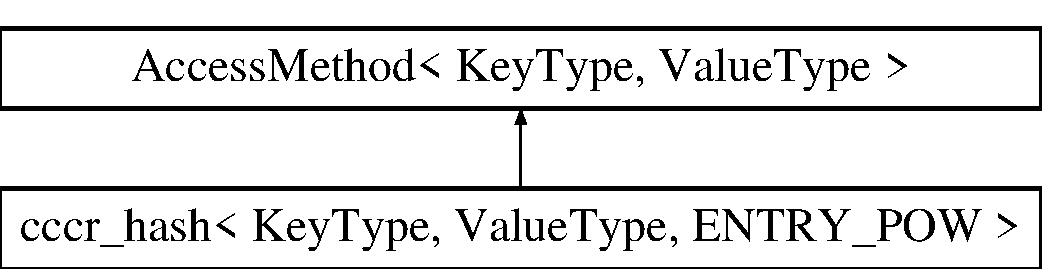
\includegraphics[height=2cm]{classcccr__hash}
\end{center}
\end{figure}
\subsection*{Public Member Functions}
\begin{CompactItemize}
\item 
\hypertarget{classcccr__hash_9f0e0f8eaf7370e7417e2fbaed88d6e6}{
bool \textbf{insert} (const DataType \&data)}
\label{classcccr__hash_9f0e0f8eaf7370e7417e2fbaed88d6e6}

\item 
\hypertarget{classcccr__hash_a4587ac348bd2b65186e5bddedd7c6a2}{
bool \textbf{update} (const DataType \&dat)}
\label{classcccr__hash_a4587ac348bd2b65186e5bddedd7c6a2}

\item 
\hypertarget{classcccr__hash_d9f201209fc37cc23afba5b07f47dbde}{
int \textbf{num\_\-items} () const }
\label{classcccr__hash_d9f201209fc37cc23afba5b07f47dbde}

\item 
\hypertarget{classcccr__hash_eddc7b7680bd29a9a17f859f291fd2da}{
void \textbf{display} (std::ostream \&os=std::cout)}
\label{classcccr__hash_eddc7b7680bd29a9a17f859f291fd2da}

\item 
\hypertarget{classcccr__hash_4016ceeb1d7fdbcb1b94132f838682f9}{
bool \textbf{insert} (const KeyType \&key, const ValueType \&v)}
\label{classcccr__hash_4016ceeb1d7fdbcb1b94132f838682f9}

\item 
\hypertarget{classcccr__hash_07d730bb1bf0c5eee4d82f1646432b30}{
ValueType $\ast$ \textbf{find} (const KeyType \&key)}
\label{classcccr__hash_07d730bb1bf0c5eee4d82f1646432b30}

\item 
\hypertarget{classcccr__hash_9a442ea53d9e4b6d429f54e6742a40be}{
bool \textbf{del} (const KeyType \&key)}
\label{classcccr__hash_9a442ea53d9e4b6d429f54e6742a40be}

\item 
\hypertarget{classcccr__hash_c5980ff3a6f52b8fcedd586598ca360b}{
bool \textbf{update} (const KeyType \&key, const ValueType \&v)}
\label{classcccr__hash_c5980ff3a6f52b8fcedd586598ca360b}

\end{CompactItemize}
\subsection*{Protected Attributes}
\begin{CompactItemize}
\item 
\hypertarget{classcccr__hash_bf34bf6bad9aa74a116546db8f584e43}{
char $\ast$ \textbf{entry\_\-} \mbox{[}ENTRY\_\-SIZE\mbox{]}}
\label{classcccr__hash_bf34bf6bad9aa74a116546db8f584e43}

\item 
\hypertarget{classcccr__hash_0e00a47602fb75b10ad2ffa93a98d53c}{
vector$<$ ValueType $>$ \textbf{dataVec\_\-}}
\label{classcccr__hash_0e00a47602fb75b10ad2ffa93a98d53c}

\item 
\hypertarget{classcccr__hash_bd2b6a257b9ca60385d9373a49b42a04}{
int \textbf{count\_\-}}
\label{classcccr__hash_bd2b6a257b9ca60385d9373a49b42a04}

\end{CompactItemize}


\subsection{Detailed Description}
\subsubsection*{template$<$typename KeyType = string, typename ValueType = NullType, size\_\-t ENTRY\_\-POW = 17$>$ class cccr\_\-hash$<$ KeyType, ValueType, ENTRY\_\-POW $>$}

\hyperlink{classcccr__hash}{cccr\_\-hash} stands for Cache-Conscious Collision Resolution String Hash Table. 

This is based on work of Nikolas Askitis and Justin Zobel, 'Cache-Conscious Collision Resolution in String Hash Tables' .On typical current machines each cache miss incurs a delay of hundreds of clock cycles while data is fetched from memory. This approach both saves space and eliminates a potential cache miss at each node access, at little cost. In experiments with large sets of strings drawn from real-world data, we show that, in comparison to standard chaining, compact-chain hash tables can yield both space savings and reductions in per-string access times. 

Definition at line 25 of file cccr\_\-hash.h.

The documentation for this class was generated from the following file:\begin{CompactItemize}
\item 
/home/Kevin/izenelib/include/am/cccr\_\-hash/cccr\_\-hash.h\end{CompactItemize}

\hypertarget{classcompletion__handler}{
\section{completion\_\-handler Class Reference}
\label{classcompletion__handler}\index{completion\_\-handler@{completion\_\-handler}}
}
Completion handler class (Loki-style).  


{\tt \#include $<$completion\_\-handler.h$>$}

\subsection*{Public Member Functions}
\begin{CompactItemize}
\item 
\hypertarget{classcompletion__handler_63b1275782e8d0a5b320e5938b09766c}{
\textbf{completion\_\-handler} (const \hyperlink{classcompletion__handler}{completion\_\-handler} \&obj)}
\label{classcompletion__handler_63b1275782e8d0a5b320e5938b09766c}

\item 
\hypertarget{classcompletion__handler_6b1cfd19f13814d73ea385ff0376ebe4}{
\hyperlink{classcompletion__handler}{completion\_\-handler} \& \textbf{operator=} (const \hyperlink{classcompletion__handler}{completion\_\-handler} \&obj)}
\label{classcompletion__handler_6b1cfd19f13814d73ea385ff0376ebe4}

\item 
\hypertarget{classcompletion__handler_cdcb747d587cfc02306d0f6447c4abed}{
void \textbf{operator()} (\hyperlink{classrequest}{request} $\ast$req)}
\label{classcompletion__handler_cdcb747d587cfc02306d0f6447c4abed}

\item 
\hypertarget{classcompletion__handler_198d05cf82bec9e1ba16828def28d3c5}{
{\footnotesize template$<$typename handler\_\-type $>$ }\\\textbf{completion\_\-handler} (const handler\_\-type \&handler\_\-\_\-)}
\label{classcompletion__handler_198d05cf82bec9e1ba16828def28d3c5}

\end{CompactItemize}


\subsection{Detailed Description}
Completion handler class (Loki-style). 

In some situations one needs to execute some actions after completion of an I/O \hyperlink{classrequest}{request}. In these cases one can use an I/O completion handler - a function object that can be passed as a parameter to asynchronous I/O calls {\tt \href{file::aread}{\tt file::aread}} and {\tt \href{file::awrite}{\tt file::awrite}} . For an example of use see \hyperlink{}{mng/test\_\-mng.cpp } 

Definition at line 38 of file completion\_\-handler.h.

The documentation for this class was generated from the following file:\begin{CompactItemize}
\item 
/home/Kevin/izenelib/include/am/blockmanager/completion\_\-handler.h\end{CompactItemize}

\hypertarget{classutil_1_1DbObj}{
\section{util::DbObj Class Reference}
\label{classutil_1_1DbObj}\index{util::DbObj@{util::DbObj}}
}
It represents the sort of objects we deal with in the BtreeFile. This is analogous to a DBT in the Berkeley DB package.  


{\tt \#include $<$DbObj.h$>$}

\subsection*{Public Member Functions}
\begin{CompactItemize}
\item 
\hypertarget{classutil_1_1DbObj_46bd24be85b68ed873f666fbd7ce7c1a}{
\hyperlink{classutil_1_1DbObj_46bd24be85b68ed873f666fbd7ce7c1a}{DbObj} (void)}
\label{classutil_1_1DbObj_46bd24be85b68ed873f666fbd7ce7c1a}

\begin{CompactList}\small\item\em Default constructor. \item\end{CompactList}\item 
\hypertarget{classutil_1_1DbObj_2e027cc833635b3605019a700d89204e}{
\hyperlink{classutil_1_1DbObj_2e027cc833635b3605019a700d89204e}{DbObj} (void $\ast$pd, size\_\-t sz)}
\label{classutil_1_1DbObj_2e027cc833635b3605019a700d89204e}

\begin{CompactList}\small\item\em Constructor taking a pointer and a size. Make a copy of the \_\-data. \item\end{CompactList}\item 
\hypertarget{classutil_1_1DbObj_720ec59f22fb852f5c3ba05eafd929bb}{
\hyperlink{classutil_1_1DbObj_720ec59f22fb852f5c3ba05eafd929bb}{DbObj} (const std::string \&s)}
\label{classutil_1_1DbObj_720ec59f22fb852f5c3ba05eafd929bb}

\begin{CompactList}\small\item\em Constructor taking a std::string reference. \item\end{CompactList}\item 
\hypertarget{classutil_1_1DbObj_040ba9bb33234312d548d872abb0f2d5}{
\hyperlink{classutil_1_1DbObj_040ba9bb33234312d548d872abb0f2d5}{DbObj} (const char $\ast$ps, size\_\-t sz=0)}
\label{classutil_1_1DbObj_040ba9bb33234312d548d872abb0f2d5}

\begin{CompactList}\small\item\em Constructor taking a (possibly) null terminated string. \item\end{CompactList}\item 
\hypertarget{classutil_1_1DbObj_62f11587e8f18e0651899a705a81cb57}{
\hyperlink{classutil_1_1DbObj_62f11587e8f18e0651899a705a81cb57}{DbObj} (unsigned long ul)}
\label{classutil_1_1DbObj_62f11587e8f18e0651899a705a81cb57}

\begin{CompactList}\small\item\em Constructor taking a 32-bit unsigned int. \item\end{CompactList}\item 
\hypertarget{classutil_1_1DbObj_6e0111e212b37df66882bdb72e9c8c6c}{
\hyperlink{classutil_1_1DbObj_6e0111e212b37df66882bdb72e9c8c6c}{DbObj} (long l)}
\label{classutil_1_1DbObj_6e0111e212b37df66882bdb72e9c8c6c}

\begin{CompactList}\small\item\em Constructor taking a 32-bit int. \item\end{CompactList}\item 
\hypertarget{classutil_1_1DbObj_457d23bfb694740c2218bd5040e35447}{
\hyperlink{classutil_1_1DbObj_457d23bfb694740c2218bd5040e35447}{DbObj} (unsigned short us)}
\label{classutil_1_1DbObj_457d23bfb694740c2218bd5040e35447}

\begin{CompactList}\small\item\em Constructor taking a 16-bit unsigned int. \item\end{CompactList}\item 
\hypertarget{classutil_1_1DbObj_bf2739aefeef09b66ff61afc3e265c80}{
\hyperlink{classutil_1_1DbObj_bf2739aefeef09b66ff61afc3e265c80}{DbObj} (short s)}
\label{classutil_1_1DbObj_bf2739aefeef09b66ff61afc3e265c80}

\begin{CompactList}\small\item\em Constructor taking a 16-bit int. \item\end{CompactList}\item 
\hypertarget{classutil_1_1DbObj_7b47bfe0c0e78e0f422ea07e2610fe14}{
\hyperlink{classutil_1_1DbObj_7b47bfe0c0e78e0f422ea07e2610fe14}{DbObj} (\hyperlink{classutil_1_1DbObj}{DbObj} \&obj)}
\label{classutil_1_1DbObj_7b47bfe0c0e78e0f422ea07e2610fe14}

\begin{CompactList}\small\item\em Copy constructor. Call the assignment operator. \item\end{CompactList}\item 
\hypertarget{classutil_1_1DbObj_19e815572aa7cfd9e46f28d5773249d4}{
\hyperlink{classutil_1_1DbObj_19e815572aa7cfd9e46f28d5773249d4}{$\sim$DbObj} ()}
\label{classutil_1_1DbObj_19e815572aa7cfd9e46f28d5773249d4}

\begin{CompactList}\small\item\em Destructor. Delete the pointer if the size is non-zero. \item\end{CompactList}\item 
\hypertarget{classutil_1_1DbObj_c31df94831fa0bd0fe3985dc7b75a537}{
\hyperlink{classutil_1_1DbObj}{DbObj} \& \hyperlink{classutil_1_1DbObj_c31df94831fa0bd0fe3985dc7b75a537}{operator=} (\hyperlink{classutil_1_1DbObj}{DbObj} \&obj)}
\label{classutil_1_1DbObj_c31df94831fa0bd0fe3985dc7b75a537}

\begin{CompactList}\small\item\em Assignment operator. Make a copy of the other object. \item\end{CompactList}\item 
\hypertarget{classutil_1_1DbObj_73bd7141e5cbb5dd8541a499d05b491f}{
bool \textbf{operator$<$=} (\hyperlink{classutil_1_1DbObj}{DbObj} \&obj)}
\label{classutil_1_1DbObj_73bd7141e5cbb5dd8541a499d05b491f}

\item 
\hypertarget{classutil_1_1DbObj_259462777be63c2c7f7aa17b57cd6294}{
const void $\ast$ \textbf{getData} () const }
\label{classutil_1_1DbObj_259462777be63c2c7f7aa17b57cd6294}

\item 
\hypertarget{classutil_1_1DbObj_46671534c7545b9a908838e82b7ec266}{
size\_\-t \textbf{getSize} () const }
\label{classutil_1_1DbObj_46671534c7545b9a908838e82b7ec266}

\item 
\hypertarget{classutil_1_1DbObj_1c4f5599227873c8116b4ceed4f17999}{
void \textbf{setData} (const void $\ast$pd, size\_\-t sz)}
\label{classutil_1_1DbObj_1c4f5599227873c8116b4ceed4f17999}

\item 
\hypertarget{classutil_1_1DbObj_b37c5a97bac8d4ba8a2ea3d8c3f02db9}{
void \textbf{display} ()}
\label{classutil_1_1DbObj_b37c5a97bac8d4ba8a2ea3d8c3f02db9}

\end{CompactItemize}


\subsection{Detailed Description}
It represents the sort of objects we deal with in the BtreeFile. This is analogous to a DBT in the Berkeley DB package. 

Definition at line 39 of file DbObj.h.

The documentation for this class was generated from the following file:\begin{CompactItemize}
\item 
/home/Kevin/izenelib/include/am/util/DbObj.h\end{CompactItemize}

\hypertarget{structdefault__completion__handler}{
\section{default\_\-completion\_\-handler Struct Reference}
\label{structdefault__completion__handler}\index{default\_\-completion\_\-handler@{default\_\-completion\_\-handler}}
}
Default completion handler class.  


{\tt \#include $<$iobase.h$>$}

\subsection*{Public Member Functions}
\begin{CompactItemize}
\item 
\hypertarget{structdefault__completion__handler_3ae7a7551771dcdd6437929b805f5651}{
void \hyperlink{structdefault__completion__handler_3ae7a7551771dcdd6437929b805f5651}{operator()} (\hyperlink{classrequest}{request} $\ast$)}
\label{structdefault__completion__handler_3ae7a7551771dcdd6437929b805f5651}

\begin{CompactList}\small\item\em An operator that does nothing. \item\end{CompactList}\end{CompactItemize}


\subsection{Detailed Description}
Default completion handler class. 

Definition at line 57 of file iobase.h.

The documentation for this struct was generated from the following file:\begin{CompactItemize}
\item 
/home/Kevin/izenelib/include/am/blockmanager/iobase.h\end{CompactItemize}

\hypertarget{classDynamicPerfectHash}{
\section{DynamicPerfectHash$<$ KeyType, ValueType, c, SM\_\-O $>$ Class Template Reference}
\label{classDynamicPerfectHash}\index{DynamicPerfectHash@{DynamicPerfectHash}}
}
{\tt \#include $<$dynamic\_\-perfect\_\-hash.hpp$>$}

Inheritance diagram for DynamicPerfectHash$<$ KeyType, ValueType, c, SM\_\-O $>$::\begin{figure}[H]
\begin{center}
\leavevmode
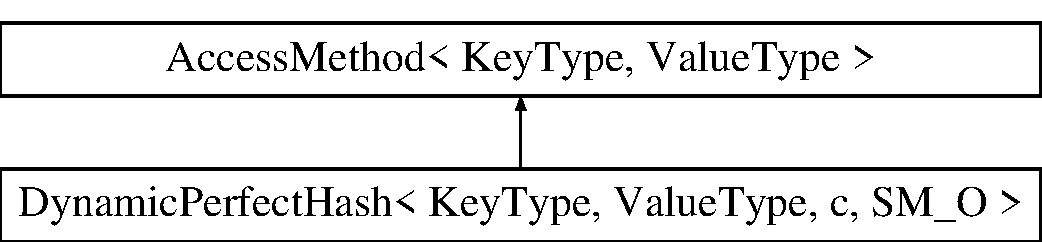
\includegraphics[height=2cm]{classDynamicPerfectHash}
\end{center}
\end{figure}
\subsection*{Classes}
\begin{CompactItemize}
\item 
class \textbf{subtable\_\-cell}
\item 
class \textbf{table\_\-cell}
\end{CompactItemize}
\subsection*{Public Member Functions}
\begin{CompactItemize}
\item 
\hypertarget{classDynamicPerfectHash_44a2a7c85a12a289c7a4dd95f6015dcc}{
uint64\_\-t \textbf{getCount} () const }
\label{classDynamicPerfectHash_44a2a7c85a12a289c7a4dd95f6015dcc}

\item 
\hypertarget{classDynamicPerfectHash_91faaff3f185c4f3d53cc171bd8fa3b5}{
uint64\_\-t \textbf{getUpdateCount} () const }
\label{classDynamicPerfectHash_91faaff3f185c4f3d53cc171bd8fa3b5}

\item 
\hypertarget{classDynamicPerfectHash_0ca61689fdfb18bf09b41bffa6d16e88}{
uint64\_\-t \textbf{getSize} () const }
\label{classDynamicPerfectHash_0ca61689fdfb18bf09b41bffa6d16e88}

\item 
\hypertarget{classDynamicPerfectHash_0466dae3d7383a7e9e5e36611be3812c}{
int \textbf{num\_\-items} () const }
\label{classDynamicPerfectHash_0466dae3d7383a7e9e5e36611be3812c}

\item 
\hypertarget{classDynamicPerfectHash_baf17e446835263f2e4ee9b85540b11f}{
virtual bool \textbf{insert} (const DataType$<$ KeyType, ValueType $>$ \&data)}
\label{classDynamicPerfectHash_baf17e446835263f2e4ee9b85540b11f}

\item 
\hypertarget{classDynamicPerfectHash_e5d36461bb755c4971870ae224e503e8}{
virtual bool \textbf{del} (const KeyType \&k)}
\label{classDynamicPerfectHash_e5d36461bb755c4971870ae224e503e8}

\item 
\hypertarget{classDynamicPerfectHash_27e311e5de18c173418035a62af293f6}{
virtual bool \textbf{update} (const DataType$<$ KeyType, ValueType $>$ \&data)}
\label{classDynamicPerfectHash_27e311e5de18c173418035a62af293f6}

\item 
\hypertarget{classDynamicPerfectHash_4d0d30a7c94465c9b154cfcfc1c951cb}{
virtual ValueType $\ast$ \textbf{find} (const KeyType \&k)}
\label{classDynamicPerfectHash_4d0d30a7c94465c9b154cfcfc1c951cb}

\item 
\hypertarget{classDynamicPerfectHash_162ff9621e8994cc5f270da673f329c8}{
bool \textbf{save} (const string \&keyFilename, const string \&valueFilename)}
\label{classDynamicPerfectHash_162ff9621e8994cc5f270da673f329c8}

\item 
\hypertarget{classDynamicPerfectHash_6127d9f252d609eff5b9b2da42efba40}{
bool \textbf{load} (const string \&keyFilename, const string \&valueFilename)}
\label{classDynamicPerfectHash_6127d9f252d609eff5b9b2da42efba40}

\end{CompactItemize}
\subsection*{Protected Member Functions}
\begin{CompactItemize}
\item 
bool \hyperlink{classDynamicPerfectHash_cdbb7a3af80d78ba2e400c531ae8319b}{rehashAll} (uint64\_\-t x, uint64\_\-t valueIdx)
\item 
\hypertarget{classDynamicPerfectHash_ae5fcc786301d81bd59881cdc050f860}{
bool \textbf{condition} ()}
\label{classDynamicPerfectHash_ae5fcc786301d81bd59881cdc050f860}

\item 
\hypertarget{classDynamicPerfectHash_a26c2436d6904064726c08b6a8a33462}{
uint64\_\-t \textbf{str\_\-hash} (const string \&x)}
\label{classDynamicPerfectHash_a26c2436d6904064726c08b6a8a33462}

\item 
\hypertarget{classDynamicPerfectHash_69ab3dcf5a7eabb0f70edd5a079f6c5d}{
uint64\_\-t \textbf{str\_\-hash} (uint64\_\-t x)}
\label{classDynamicPerfectHash_69ab3dcf5a7eabb0f70edd5a079f6c5d}

\item 
\hypertarget{classDynamicPerfectHash_cf4ec08043a93b0e8166c035eb2d0c73}{
uint64\_\-t \textbf{hashFunc} (uint64\_\-t a, uint64\_\-t b, uint64\_\-t p, uint64\_\-t s, const uint64\_\-t \&x)}
\label{classDynamicPerfectHash_cf4ec08043a93b0e8166c035eb2d0c73}

\item 
\hypertarget{classDynamicPerfectHash_2a0c5701a610369dc161daeba71be0b9}{
void \textbf{adjustSubTable} (uint64\_\-t idx, const subtable\_\-cell \&x=subtable\_\-cell(0,-1))}
\label{classDynamicPerfectHash_2a0c5701a610369dc161daeba71be0b9}

\item 
\hypertarget{classDynamicPerfectHash_66e0a5280dea2453fb041bb6dfb6b6dd}{
void \textbf{deleteAll} ()}
\label{classDynamicPerfectHash_66e0a5280dea2453fb041bb6dfb6b6dd}

\item 
\hypertarget{classDynamicPerfectHash_726ca036dba3fb4cf9efb2d7ae894ccf}{
void \textbf{deleteSubT} (uint64\_\-t idx)}
\label{classDynamicPerfectHash_726ca036dba3fb4cf9efb2d7ae894ccf}

\end{CompactItemize}
\subsection*{Static Protected Member Functions}
\begin{CompactItemize}
\item 
\hypertarget{classDynamicPerfectHash_06c1dca453cee284551ecd75fa76c1b1}{
static void \textbf{random\_\-param} (uint64\_\-t \&a, uint64\_\-t \&b, uint64\_\-t \&p)}
\label{classDynamicPerfectHash_06c1dca453cee284551ecd75fa76c1b1}

\end{CompactItemize}
\subsection*{Protected Attributes}
\begin{CompactItemize}
\item 
\hypertarget{classDynamicPerfectHash_acbb9741f2d1e0f85acd95252a9733bb}{
table\_\-cell $\ast$ \textbf{pMainT\_\-}}
\label{classDynamicPerfectHash_acbb9741f2d1e0f85acd95252a9733bb}

\item 
\hypertarget{classDynamicPerfectHash_e916a52b5175cef011b7cd7d4ed9757b}{
uint64\_\-t \textbf{count\_\-}}
\label{classDynamicPerfectHash_e916a52b5175cef011b7cd7d4ed9757b}

\item 
\hypertarget{classDynamicPerfectHash_746d548346ed75fe9216b903288d942b}{
uint64\_\-t \textbf{update\_\-count\_\-}}
\label{classDynamicPerfectHash_746d548346ed75fe9216b903288d942b}

\item 
\hypertarget{classDynamicPerfectHash_4092248a8b7aa784d48365c35e35a3ef}{
uint64\_\-t \textbf{M\_\-}}
\label{classDynamicPerfectHash_4092248a8b7aa784d48365c35e35a3ef}

\item 
\hypertarget{classDynamicPerfectHash_6eeaeef7a6d2eee468376ddfa27193fa}{
uint64\_\-t \textbf{mainT\_\-size\_\-}}
\label{classDynamicPerfectHash_6eeaeef7a6d2eee468376ddfa27193fa}

\item 
\hypertarget{classDynamicPerfectHash_3eebf60a66d98de38298a3c30a81aef2}{
uint64\_\-t \textbf{main\_\-k\_\-}}
\label{classDynamicPerfectHash_3eebf60a66d98de38298a3c30a81aef2}

\item 
\hypertarget{classDynamicPerfectHash_979c74273ea13bdfbb4b75f9f5eb2948}{
uint64\_\-t \textbf{main\_\-u\_\-}}
\label{classDynamicPerfectHash_979c74273ea13bdfbb4b75f9f5eb2948}

\item 
\hypertarget{classDynamicPerfectHash_f21212ae2ec837a42784858a22d95d09}{
uint64\_\-t \textbf{main\_\-p\_\-}}
\label{classDynamicPerfectHash_f21212ae2ec837a42784858a22d95d09}

\item 
\hypertarget{classDynamicPerfectHash_6b0a1648f26e87d0c2bfb071b99e0724}{
vector$<$ ValueType $>$ \textbf{dataVec\_\-}}
\label{classDynamicPerfectHash_6b0a1648f26e87d0c2bfb071b99e0724}

\item 
\hypertarget{classDynamicPerfectHash_8cbc08d724ea9be3431fc5080cfb7c2f}{
uint64\_\-t \textbf{sum\_\-s\_\-}}
\label{classDynamicPerfectHash_8cbc08d724ea9be3431fc5080cfb7c2f}

\end{CompactItemize}
\subsection*{Friends}
\begin{CompactItemize}
\item 
\hypertarget{classDynamicPerfectHash_d6b3ef7ecb2e9975d8022514f68f74f5}{
ostream \& \textbf{operator$<$$<$} (ostream \&os, const \hyperlink{classDynamicPerfectHash}{SelfType} \&node)}
\label{classDynamicPerfectHash_d6b3ef7ecb2e9975d8022514f68f74f5}

\end{CompactItemize}


\subsection{Detailed Description}
\subsubsection*{template$<$class KeyType = uint32\_\-t, class ValueType = uint32\_\-t, uint32\_\-t c = 2500000, uint32\_\-t SM\_\-O = 1$>$ class DynamicPerfectHash$<$ KeyType, ValueType, c, SM\_\-O $>$}

This work is based on Martin's paper 'Dynammic Perfect Hashing: Upper and Lower Bonds' in 1990. 

Definition at line 30 of file dynamic\_\-perfect\_\-hash.hpp.

\subsection{Member Function Documentation}
\hypertarget{classDynamicPerfectHash_cdbb7a3af80d78ba2e400c531ae8319b}{
\index{DynamicPerfectHash@{DynamicPerfectHash}!rehashAll@{rehashAll}}
\index{rehashAll@{rehashAll}!DynamicPerfectHash@{DynamicPerfectHash}}
\subsubsection[{rehashAll}]{\setlength{\rightskip}{0pt plus 5cm}template$<$class KeyType  = uint32\_\-t, class ValueType  = uint32\_\-t, uint32\_\-t c = 2500000, uint32\_\-t SM\_\-O = 1$>$ bool {\bf DynamicPerfectHash}$<$ KeyType, ValueType, c, SM\_\-O $>$::rehashAll (uint64\_\-t {\em x}, \/  uint64\_\-t {\em valueIdx})\hspace{0.3cm}{\tt  \mbox{[}inline, protected\mbox{]}}}}
\label{classDynamicPerfectHash_cdbb7a3af80d78ba2e400c531ae8319b}


RehashAll(x) is either called by insert(x) or del(x), and then x=-1. rehashAll(x) build a new table for all elements currently in table. 

Definition at line 521 of file dynamic\_\-perfect\_\-hash.hpp.

The documentation for this class was generated from the following file:\begin{CompactItemize}
\item 
/home/Kevin/izenelib/include/am/dynamic\_\-perfect\_\-hash/dynamic\_\-perfect\_\-hash.hpp\end{CompactItemize}

\hypertarget{classelement__block}{
\section{element\_\-block$<$ T, Size\_\- $>$ Class Template Reference}
\label{classelement__block}\index{element\_\-block@{element\_\-block}}
}
Contains data elements for {\tt \hyperlink{classtyped__block}{typed\_\-block}} , not intended for direct use.  


{\tt \#include $<$main.h$>$}

Inheritance diagram for element\_\-block$<$ T, Size\_\- $>$::\begin{figure}[H]
\begin{center}
\leavevmode
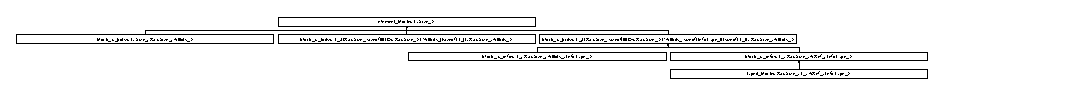
\includegraphics[height=0.824742cm]{classelement__block}
\end{center}
\end{figure}
\subsection*{Public Types}
\begin{CompactItemize}
\item 
enum \{ \hyperlink{group__mnglayer_gg2c6c9f26f6ba7bd45841bb125b90e04f5fdb4b66f1c64a4b69f23756713341f2}{size} =  Size\_\-
 \}
\item 
\hypertarget{classelement__block_0f3e4d93c44656acb473cde14318bacc}{
typedef T \textbf{type}}
\label{classelement__block_0f3e4d93c44656acb473cde14318bacc}

\item 
\hypertarget{group__mnglayer_gf4b942e8fd7f45f98e878658dd9d5eb3}{
typedef T \textbf{value\_\-type}}
\label{group__mnglayer_gf4b942e8fd7f45f98e878658dd9d5eb3}

\item 
\hypertarget{group__mnglayer_g440dde951fbd48acb83efcb7eb146fb7}{
typedef T \& \textbf{reference}}
\label{group__mnglayer_g440dde951fbd48acb83efcb7eb146fb7}

\item 
\hypertarget{group__mnglayer_gf5d43971860fb25f4cd591fe678bfc41}{
typedef const T \& \textbf{const\_\-reference}}
\label{group__mnglayer_gf5d43971860fb25f4cd591fe678bfc41}

\item 
\hypertarget{group__mnglayer_g0a2a1c6bc4bdad79df97c4fea68524b8}{
typedef type $\ast$ \textbf{pointer}}
\label{group__mnglayer_g0a2a1c6bc4bdad79df97c4fea68524b8}

\item 
\hypertarget{group__mnglayer_gc468b1fa2d879f091debc2d9fe0b329e}{
typedef pointer \textbf{iterator}}
\label{group__mnglayer_gc468b1fa2d879f091debc2d9fe0b329e}

\item 
\hypertarget{group__mnglayer_g0e51dca212a92bf8fe8f0ab48d93e915}{
typedef const type $\ast$ \textbf{const\_\-iterator}}
\label{group__mnglayer_g0e51dca212a92bf8fe8f0ab48d93e915}

\end{CompactItemize}
\subsection*{Public Member Functions}
\begin{CompactItemize}
\item 
\hypertarget{group__mnglayer_gb90a755bf03c0113dd37014f6f8dc53d}{
reference \hyperlink{group__mnglayer_gb90a755bf03c0113dd37014f6f8dc53d}{operator\mbox{[}$\,$\mbox{]}} (int i)}
\label{group__mnglayer_gb90a755bf03c0113dd37014f6f8dc53d}

\begin{CompactList}\small\item\em An operator to access elements in the block. \item\end{CompactList}\item 
\hypertarget{group__mnglayer_gcae10d17bbcc8af7c10ef052283aa7e9}{
iterator \hyperlink{group__mnglayer_gcae10d17bbcc8af7c10ef052283aa7e9}{begin} ()}
\label{group__mnglayer_gcae10d17bbcc8af7c10ef052283aa7e9}

\begin{CompactList}\small\item\em Returns {\tt iterator} pointing to the first element. \item\end{CompactList}\item 
\hypertarget{group__mnglayer_gd5a7afcaa6b7c4762e831c43648fb5af}{
const\_\-iterator \hyperlink{group__mnglayer_gd5a7afcaa6b7c4762e831c43648fb5af}{begin} () const }
\label{group__mnglayer_gd5a7afcaa6b7c4762e831c43648fb5af}

\begin{CompactList}\small\item\em Returns {\tt const\_\-iterator} pointing to the first element. \item\end{CompactList}\item 
\hypertarget{group__mnglayer_gbc98bc4725bb92fc30627633816097ef}{
const\_\-iterator \hyperlink{group__mnglayer_gbc98bc4725bb92fc30627633816097ef}{cbegin} () const }
\label{group__mnglayer_gbc98bc4725bb92fc30627633816097ef}

\begin{CompactList}\small\item\em Returns {\tt const\_\-iterator} pointing to the first element. \item\end{CompactList}\item 
\hypertarget{group__mnglayer_g1b89fe04df5d14b3e1cf536298331413}{
iterator \hyperlink{group__mnglayer_g1b89fe04df5d14b3e1cf536298331413}{end} ()}
\label{group__mnglayer_g1b89fe04df5d14b3e1cf536298331413}

\begin{CompactList}\small\item\em Returns {\tt iterator} pointing to the end element. \item\end{CompactList}\item 
\hypertarget{group__mnglayer_g75cecec83bf923364d5144e53d10a1ff}{
const\_\-iterator \hyperlink{group__mnglayer_g75cecec83bf923364d5144e53d10a1ff}{end} () const }
\label{group__mnglayer_g75cecec83bf923364d5144e53d10a1ff}

\begin{CompactList}\small\item\em Returns {\tt const\_\-iterator} pointing to the end element. \item\end{CompactList}\item 
\hypertarget{group__mnglayer_g792762a9693c0dcc3ff53d316fa8d9d9}{
const\_\-iterator \hyperlink{group__mnglayer_g792762a9693c0dcc3ff53d316fa8d9d9}{cend} () const }
\label{group__mnglayer_g792762a9693c0dcc3ff53d316fa8d9d9}

\begin{CompactList}\small\item\em Returns {\tt const\_\-iterator} pointing to the end element. \item\end{CompactList}\end{CompactItemize}
\subsection*{Public Attributes}
\begin{CompactItemize}
\item 
\hypertarget{group__mnglayer_g3c39c144c1d556157c908950f62cf168}{
T \hyperlink{group__mnglayer_g3c39c144c1d556157c908950f62cf168}{elem} \mbox{[}size\mbox{]}}
\label{group__mnglayer_g3c39c144c1d556157c908950f62cf168}

\begin{CompactList}\small\item\em Array of elements of type T. \item\end{CompactList}\end{CompactItemize}


\subsection{Detailed Description}
\subsubsection*{template$<$class T, unsigned Size\_\-$>$ class element\_\-block$<$ T, Size\_\- $>$}

Contains data elements for {\tt \hyperlink{classtyped__block}{typed\_\-block}} , not intended for direct use. 

Definition at line 127 of file main.h.

The documentation for this class was generated from the following file:\begin{CompactItemize}
\item 
/home/Kevin/izenelib/include/am/blockmanager/main.h\end{CompactItemize}

\hypertarget{classfile}{
\section{file Class Reference}
\label{classfile}\index{file@{file}}
}
Defines interface of \hyperlink{classfile}{file}.  


{\tt \#include $<$iobase.h$>$}

Inherited by boostfd\_\-file.

\subsection*{Public Types}
\begin{CompactItemize}
\item 
enum \hyperlink{group__iolayer_ge71b15e0014e7ce4dc13c8f83aa97582}{open\_\-mode} \{ \par
\hyperlink{group__iolayer_gge71b15e0014e7ce4dc13c8f83aa97582ac58f1566e053cf5f8ee9dcb5f97b82b}{RDONLY} =  1, 
\hyperlink{group__iolayer_gge71b15e0014e7ce4dc13c8f83aa97582de40e8cbe66eb259ed5378c7d13b4f69}{WRONLY} =  2, 
\hyperlink{group__iolayer_gge71b15e0014e7ce4dc13c8f83aa97582afcab766b3f436a66049b850ef7efb5c}{RDWR} =  4, 
\hyperlink{group__iolayer_gge71b15e0014e7ce4dc13c8f83aa97582971314bb8ab4fa48a078a4164c704edd}{CREAT} =  8, 
\par
\hyperlink{group__iolayer_gge71b15e0014e7ce4dc13c8f83aa97582e1e222042131ddbb85b2bd3fc0f80653}{DIRECT} =  16, 
\hyperlink{group__iolayer_gge71b15e0014e7ce4dc13c8f83aa975828842a94419a50b809fdead40a130785d}{TRUNC} =  32
 \}
\begin{CompactList}\small\item\em Definition of acceptable \hyperlink{classfile}{file} open modes. \item\end{CompactList}\end{CompactItemize}
\subsection*{Public Member Functions}
\begin{CompactItemize}
\item 
virtual \hyperlink{classrequest__ptr}{request\_\-ptr} \hyperlink{group__iolayer_gccc17bdde11461510dce18cefec5d207}{aread} (void $\ast$buffer, int64\_\-t pos, size\_\-t bytes, \hyperlink{classcompletion__handler}{completion\_\-handler} on\_\-cmpl)=0
\begin{CompactList}\small\item\em Schedules asynchronous read \hyperlink{classrequest}{request} to the \hyperlink{classfile}{file}. \item\end{CompactList}\item 
virtual \hyperlink{classrequest__ptr}{request\_\-ptr} \hyperlink{group__iolayer_g5c15b0b96abcfc0b06bb906afbf1dd2b}{awrite} (void $\ast$buffer, int64\_\-t pos, size\_\-t bytes, \hyperlink{classcompletion__handler}{completion\_\-handler} on\_\-cmpl)=0
\begin{CompactList}\small\item\em Schedules asynchronous write \hyperlink{classrequest}{request} to the \hyperlink{classfile}{file}. \item\end{CompactList}\item 
virtual void \hyperlink{group__iolayer_g0388ba482ccd9be978edef3d54e2e41c}{set\_\-size} (int64\_\-t newsize)=0
\begin{CompactList}\small\item\em Changes the size of the \hyperlink{classfile}{file}. \item\end{CompactList}\item 
virtual int64\_\-t \hyperlink{group__iolayer_g452fdcecf86299ffda1aba728a28c98d}{size} ()=0
\begin{CompactList}\small\item\em Returns size of the \hyperlink{classfile}{file}. \item\end{CompactList}\item 
\hypertarget{group__iolayer_g27be6a3162808bae88906d6f7b383fff}{
virtual void \hyperlink{group__iolayer_g27be6a3162808bae88906d6f7b383fff}{lock} ()}
\label{group__iolayer_g27be6a3162808bae88906d6f7b383fff}

\begin{CompactList}\small\item\em Locks \hyperlink{classfile}{file} for reading and writing. \item\end{CompactList}\item 
\hypertarget{group__iolayer_g1bb12d404c9a31564ba2c3c3e870ac49}{
virtual void \hyperlink{group__iolayer_g1bb12d404c9a31564ba2c3c3e870ac49}{delete\_\-region} (int64\_\-t offset, unsigned\_\-type size)}
\label{group__iolayer_g1bb12d404c9a31564ba2c3c3e870ac49}

\begin{CompactList}\small\item\em Some specialized \hyperlink{classfile}{file} types may need to know freed regions. \item\end{CompactList}\end{CompactItemize}
\subsection*{Protected Member Functions}
\begin{CompactItemize}
\item 
\hyperlink{classfile_22090815b0614f552f2cb2cc8f170572}{file} ()
\begin{CompactList}\small\item\em Initializes \hyperlink{classfile}{file} object. \item\end{CompactList}\end{CompactItemize}


\subsection{Detailed Description}
Defines interface of \hyperlink{classfile}{file}. 

It is a base class for different implementations that might base on various \hyperlink{classfile}{file} systems or even remote storage interfaces 

Definition at line 67 of file iobase.h.

\subsection{Constructor \& Destructor Documentation}
\hypertarget{classfile_22090815b0614f552f2cb2cc8f170572}{
\index{file@{file}!file@{file}}
\index{file@{file}!file@{file}}
\subsubsection[{file}]{\setlength{\rightskip}{0pt plus 5cm}file::file ()\hspace{0.3cm}{\tt  \mbox{[}inline, protected\mbox{]}}}}
\label{classfile_22090815b0614f552f2cb2cc8f170572}


Initializes \hyperlink{classfile}{file} object. 

\begin{Desc}
\item[Parameters:]
\begin{description}
\item[{\em \_\-id}]\hyperlink{classfile}{file} identifier \end{description}
\end{Desc}
\begin{Desc}
\item[Remarks:]Called in implementations of \hyperlink{classfile}{file} \end{Desc}


Definition at line 74 of file iobase.h.

The documentation for this class was generated from the following file:\begin{CompactItemize}
\item 
/home/Kevin/izenelib/include/am/blockmanager/iobase.h\end{CompactItemize}

\hypertarget{classLinearHashTable}{
\section{LinearHashTable$<$ KeyType, ValueType, LockType $>$ Class Template Reference}
\label{classLinearHashTable}\index{LinearHashTable@{LinearHashTable}}
}
\hyperlink{classLinearHashTable}{LinearHashTable} is based on Per-Ake Larson's work, Dynamic Hash Tables.  


{\tt \#include $<$LinearHashTable.h$>$}

Inheritance diagram for LinearHashTable$<$ KeyType, ValueType, LockType $>$::\begin{figure}[H]
\begin{center}
\leavevmode
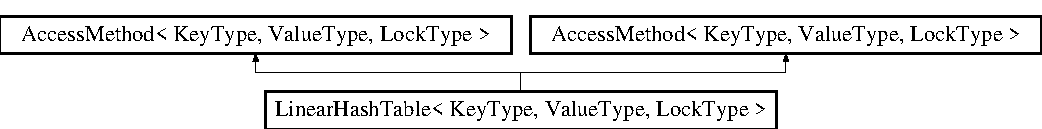
\includegraphics[height=1.7284cm]{classLinearHashTable}
\end{center}
\end{figure}
\subsection*{Public Member Functions}
\begin{CompactItemize}
\item 
\hypertarget{classLinearHashTable_bf7283c1702c43b8a8ea62974c4f8c3b}{
\hyperlink{classLinearHashTable_bf7283c1702c43b8a8ea62974c4f8c3b}{LinearHashTable} ()}
\label{classLinearHashTable_bf7283c1702c43b8a8ea62974c4f8c3b}

\begin{CompactList}\small\item\em Default constructor, Initialize member variables. \item\end{CompactList}\item 
\hypertarget{classLinearHashTable_71ba4421ab8d3e78ac12b1bbf064c339}{
\hyperlink{classLinearHashTable_71ba4421ab8d3e78ac12b1bbf064c339}{LinearHashTable} (double minloadf, double maxloadf)}
\label{classLinearHashTable_71ba4421ab8d3e78ac12b1bbf064c339}

\begin{CompactList}\small\item\em The constructor. \item\end{CompactList}\item 
\hypertarget{classLinearHashTable_5ebdebd06837f32e434a7ce7d2ce8897}{
\hyperlink{classLinearHashTable_5ebdebd06837f32e434a7ce7d2ce8897}{$\sim$LinearHashTable} ()}
\label{classLinearHashTable_5ebdebd06837f32e434a7ce7d2ce8897}

\begin{CompactList}\small\item\em The destructor. \item\end{CompactList}\item 
\hypertarget{classLinearHashTable_5072a29db252e08a74a65a7f8b12c8a6}{
void \hyperlink{classLinearHashTable_5072a29db252e08a74a65a7f8b12c8a6}{release} ()}
\label{classLinearHashTable_5072a29db252e08a74a65a7f8b12c8a6}

\begin{CompactList}\small\item\em Releases the \hyperlink{classLinearHashTable}{LinearHashTable} object. \item\end{CompactList}\item 
\hypertarget{classLinearHashTable_a8853f851d5439c3e2c13f61af532e9a}{
int \textbf{num\_\-items} () const }
\label{classLinearHashTable_a8853f851d5439c3e2c13f61af532e9a}

\item 
\hypertarget{classLinearHashTable_9f34587eba1ac1dcbc75d91b69935a2a}{
int \textbf{get\_\-current\_\-items} ()}
\label{classLinearHashTable_9f34587eba1ac1dcbc75d91b69935a2a}

\item 
\hypertarget{classLinearHashTable_9a63048edd94def6f70b05f949067dc9}{
int \textbf{num\_\-buckets} () const }
\label{classLinearHashTable_9a63048edd94def6f70b05f949067dc9}

\item 
\hypertarget{classLinearHashTable_c045c16812af47da63e808a38f3797ef}{
ValueType $\ast$ \textbf{find} (const KeyType \&key)}
\label{classLinearHashTable_c045c16812af47da63e808a38f3797ef}

\item 
\hypertarget{classLinearHashTable_a614f36856d95f4a0b0c60114c51067f}{
const ValueType $\ast$ \textbf{find} (const KeyType \&key) const }
\label{classLinearHashTable_a614f36856d95f4a0b0c60114c51067f}

\item 
bool \hyperlink{classLinearHashTable_6cfa4db9583b1dd5615cedfb2220e7f3}{insert} (const DataType \&elem)
\item 
\hypertarget{classLinearHashTable_1a7ce5b3a45b5d15e10c39621b4dd0ff}{
bool \textbf{insert} (const KeyType \&key, const ValueType \&value)}
\label{classLinearHashTable_1a7ce5b3a45b5d15e10c39621b4dd0ff}

\item 
bool \hyperlink{classLinearHashTable_4008d6c42a099654c137d212f83176ae}{del} (const KeyType \&key)
\begin{CompactList}\small\item\em updata an item with given key, if it not exist, insert it directly. \item\end{CompactList}\item 
\hypertarget{classLinearHashTable_9c1b4c961b7b19ee6a90dcff1a542879}{
void \hyperlink{classLinearHashTable_9c1b4c961b7b19ee6a90dcff1a542879}{display} (std::ostream \&stream) const }
\label{classLinearHashTable_9c1b4c961b7b19ee6a90dcff1a542879}

\begin{CompactList}\small\item\em Display information about linear hashing for debug. \item\end{CompactList}\item 
\hypertarget{classLinearHashTable_d43140773375a24fab89a00f94718228}{
{\footnotesize template$<$typename Archive $>$ }\\void \textbf{save} (Archive \&ar, const unsigned int version=0) const }
\label{classLinearHashTable_d43140773375a24fab89a00f94718228}

\item 
\hypertarget{classLinearHashTable_2034e3f01b1635d606a0cac7473c44fa}{
{\footnotesize template$<$typename Archive $>$ }\\void \textbf{load} (Archive \&ar, const unsigned int version=0)}
\label{classLinearHashTable_2034e3f01b1635d606a0cac7473c44fa}

\item 
\hypertarget{classLinearHashTable_d6d8cf1cadf308a9046bc840258421ef}{
void \textbf{copyTo} (AccessMethod$<$ KeyType, ValueType, LockType $>$ \&am) const }
\label{classLinearHashTable_d6d8cf1cadf308a9046bc840258421ef}

\item 
\hypertarget{classLinearHashTable_1e308125876860695f39903999c00002}{
virtual bool \textbf{insert} (const DataType$<$ KeyType, ValueType $>$ \&data)}
\label{classLinearHashTable_1e308125876860695f39903999c00002}

\item 
\hypertarget{classLinearHashTable_36409b1f8b938bff754c78b1e6a82624}{
virtual bool \textbf{update} (const DataType$<$ KeyType, ValueType $>$ \&data)}
\label{classLinearHashTable_36409b1f8b938bff754c78b1e6a82624}

\item 
\hypertarget{classLinearHashTable_112a278af50345335a469d88718fbe1a}{
virtual ValueType $\ast$ \textbf{find} (const KeyType \&key)}
\label{classLinearHashTable_112a278af50345335a469d88718fbe1a}

\item 
\hypertarget{classLinearHashTable_60a358efba34efa531f76b6d1a1b2389}{
virtual bool \textbf{del} (const KeyType \&key)}
\label{classLinearHashTable_60a358efba34efa531f76b6d1a1b2389}

\end{CompactItemize}
\subsection*{Protected Member Functions}
\begin{CompactItemize}
\item 
\hypertarget{classLinearHashTable_e69f1092a593508959afc20a8fac7e37}{
int \hyperlink{classLinearHashTable_e69f1092a593508959afc20a8fac7e37}{hash} (const KeyType \&key) const }
\label{classLinearHashTable_e69f1092a593508959afc20a8fac7e37}

\begin{CompactList}\small\item\em Returns a hash value of a key. \item\end{CompactList}\item 
\hypertarget{classLinearHashTable_2eaad3e86cbc65ca346fac49c68c9681}{
void \hyperlink{classLinearHashTable_2eaad3e86cbc65ca346fac49c68c9681}{expand\_\-table} ()}
\label{classLinearHashTable_2eaad3e86cbc65ca346fac49c68c9681}

\begin{CompactList}\small\item\em Expands the table. \item\end{CompactList}\item 
\hypertarget{classLinearHashTable_1f5e14b52ff8aa9a3ee6fce2628dcf01}{
void \hyperlink{classLinearHashTable_1f5e14b52ff8aa9a3ee6fce2628dcf01}{contract\_\-table} ()}
\label{classLinearHashTable_1f5e14b52ff8aa9a3ee6fce2628dcf01}

\begin{CompactList}\small\item\em Contracts the table, exactly the opposite of \hyperlink{classLinearHashTable_2eaad3e86cbc65ca346fac49c68c9681}{expand\_\-table()}. \item\end{CompactList}\item 
\hypertarget{classLinearHashTable_903d29e1f557b251cb00e9b89a303356}{
void \textbf{init} ()}
\label{classLinearHashTable_903d29e1f557b251cb00e9b89a303356}

\end{CompactItemize}


\subsection{Detailed Description}
\subsubsection*{template$<$typename KeyType, typename ValueType, typename LockType = NullLock$>$ class LinearHashTable$<$ KeyType, ValueType, LockType $>$}

\hyperlink{classLinearHashTable}{LinearHashTable} is based on Per-Ake Larson's work, Dynamic Hash Tables. 

It is the fastest hash table that I know and have implemented. There are several parameters to tune for faster performance. The min/max load factor is vital in the tuning. The segment and directory size could be important factors but have not been experimented.

One idea is to expedite the growth/shrink process by expanding or contracting more than one buckets. It is not clear yet whether such a move would be beneficial. 

Definition at line 89 of file LinearHashTable.h.

\subsection{Member Function Documentation}
\hypertarget{classLinearHashTable_4008d6c42a099654c137d212f83176ae}{
\index{LinearHashTable@{LinearHashTable}!del@{del}}
\index{del@{del}!LinearHashTable@{LinearHashTable}}
\subsubsection[{del}]{\setlength{\rightskip}{0pt plus 5cm}template$<$typename KeyType , typename ValueType , typename LockType $>$ bool {\bf LinearHashTable}$<$ KeyType, ValueType, LockType $>$::del (const KeyType \& {\em key})\hspace{0.3cm}{\tt  \mbox{[}inline\mbox{]}}}}
\label{classLinearHashTable_4008d6c42a099654c137d212f83176ae}


updata an item with given key, if it not exist, insert it directly. 

Deletes an DataType.

updata an item with given key, if it not exist, insert it directly.



\begin{Code}\begin{verbatim}        Comments: This method takes the ownership and deletes the data itself
            when successful.
\end{verbatim}
\end{Code}

 

Definition at line 471 of file LinearHashTable.h.\hypertarget{classLinearHashTable_6cfa4db9583b1dd5615cedfb2220e7f3}{
\index{LinearHashTable@{LinearHashTable}!insert@{insert}}
\index{insert@{insert}!LinearHashTable@{LinearHashTable}}
\subsubsection[{insert}]{\setlength{\rightskip}{0pt plus 5cm}template$<$typename KeyType , typename ValueType , typename LockType $>$ bool {\bf LinearHashTable}$<$ KeyType, ValueType, LockType $>$::insert (const DataType \& {\em elem})\hspace{0.3cm}{\tt  \mbox{[}inline\mbox{]}}}}
\label{classLinearHashTable_6cfa4db9583b1dd5615cedfb2220e7f3}


Inserts an DataType (takes a pointer). 

Definition at line 427 of file LinearHashTable.h.

The documentation for this class was generated from the following files:\begin{CompactItemize}
\item 
/home/Kevin/izenelib/include/am/fromylib/\hyperlink{LinearHashTable_8h}{LinearHashTable.h}\item 
/home/Kevin/izenelib/include/am/linear\_\-hash\_\-table/linearHashTable.hpp\end{CompactItemize}

\hypertarget{classLinearHashTable_3_01ValueType_00_01KeyType_00_01MemStorage_00_01SEGMENT__SIZE_00_01DIRECTORc7a065a47b9854d6d22bcaeeb634c1b3}{
\section{LinearHashTable$<$ ValueType, KeyType, MemStorage, SEGMENT\_\-SIZE, DIRECTORY\_\-SIZE, expandFctrPerc, shrinkFctrPerc, LockType, HashFuncType $>$ Class Template Reference}
\label{classLinearHashTable_3_01ValueType_00_01KeyType_00_01MemStorage_00_01SEGMENT__SIZE_00_01DIRECTORc7a065a47b9854d6d22bcaeeb634c1b3}\index{LinearHashTable$<$ ValueType, KeyType, MemStorage, SEGMENT\_\-SIZE, DIRECTORY\_\-SIZE, expandFctrPerc, shrinkFctrPerc, LockType, HashFuncType $>$@{LinearHashTable$<$ ValueType, KeyType, MemStorage, SEGMENT\_\-SIZE, DIRECTORY\_\-SIZE, expandFctrPerc, shrinkFctrPerc, LockType, HashFuncType $>$}}
}
\hyperlink{classLinearHashTable}{LinearHashTable} is based on Per-Ake Larson's work, Dynamic Hash Tables.  


{\tt \#include $<$linearHashTable.hpp$>$}

Inheritance diagram for LinearHashTable$<$ ValueType, KeyType, MemStorage, SEGMENT\_\-SIZE, DIRECTORY\_\-SIZE, expandFctrPerc, shrinkFctrPerc, LockType, HashFuncType $>$::\begin{figure}[H]
\begin{center}
\leavevmode
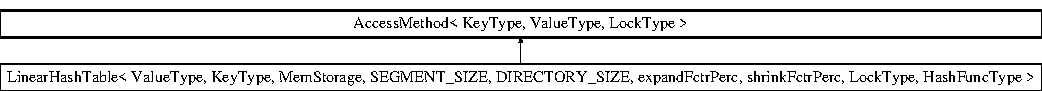
\includegraphics[height=1.22942cm]{classLinearHashTable_3_01ValueType_00_01KeyType_00_01MemStorage_00_01SEGMENT__SIZE_00_01DIRECTORc7a065a47b9854d6d22bcaeeb634c1b3}
\end{center}
\end{figure}
\subsection*{Classes}
\begin{CompactItemize}
\item 
class \textbf{LHTElem}
\item 
class \textbf{Segment}
\end{CompactItemize}
\subsection*{Public Types}
\begin{CompactItemize}
\item 
\hypertarget{classLinearHashTable_3_01ValueType_00_01KeyType_00_01MemStorage_00_01SEGMENT__SIZE_00_01DIRECTORc7a065a47b9854d6d22bcaeeb634c1b3_6ecf1f7c35f93e5eeab12afaf45965c6}{
typedef \hyperlink{classLinearHashTable}{LinearHashTable}$<$ ValueType, KeyType, MemStorage, SEGMENT\_\-SIZE, DIRECTORY\_\-SIZE, expandFctrPerc, shrinkFctrPerc, LockType, HashFuncType $>$ \textbf{Self}}
\label{classLinearHashTable_3_01ValueType_00_01KeyType_00_01MemStorage_00_01SEGMENT__SIZE_00_01DIRECTORc7a065a47b9854d6d22bcaeeb634c1b3_6ecf1f7c35f93e5eeab12afaf45965c6}

\end{CompactItemize}
\subsection*{Public Member Functions}
\begin{CompactItemize}
\item 
\hypertarget{classLinearHashTable_3_01ValueType_00_01KeyType_00_01MemStorage_00_01SEGMENT__SIZE_00_01DIRECTORc7a065a47b9854d6d22bcaeeb634c1b3_0f170ef320ad190e7c224fdbd2a2fb29}{
\hyperlink{classLinearHashTable_3_01ValueType_00_01KeyType_00_01MemStorage_00_01SEGMENT__SIZE_00_01DIRECTORc7a065a47b9854d6d22bcaeeb634c1b3_0f170ef320ad190e7c224fdbd2a2fb29}{LinearHashTable} ()}
\label{classLinearHashTable_3_01ValueType_00_01KeyType_00_01MemStorage_00_01SEGMENT__SIZE_00_01DIRECTORc7a065a47b9854d6d22bcaeeb634c1b3_0f170ef320ad190e7c224fdbd2a2fb29}

\begin{CompactList}\small\item\em Default constructor, Initialize member variables. \item\end{CompactList}\item 
\hypertarget{classLinearHashTable_3_01ValueType_00_01KeyType_00_01MemStorage_00_01SEGMENT__SIZE_00_01DIRECTORc7a065a47b9854d6d22bcaeeb634c1b3_829572e5b1e66b65039b8672c59d8c70}{
\hyperlink{classLinearHashTable_3_01ValueType_00_01KeyType_00_01MemStorage_00_01SEGMENT__SIZE_00_01DIRECTORc7a065a47b9854d6d22bcaeeb634c1b3_829572e5b1e66b65039b8672c59d8c70}{$\sim$LinearHashTable} ()}
\label{classLinearHashTable_3_01ValueType_00_01KeyType_00_01MemStorage_00_01SEGMENT__SIZE_00_01DIRECTORc7a065a47b9854d6d22bcaeeb634c1b3_829572e5b1e66b65039b8672c59d8c70}

\begin{CompactList}\small\item\em The destructor. \item\end{CompactList}\item 
\hypertarget{classLinearHashTable_3_01ValueType_00_01KeyType_00_01MemStorage_00_01SEGMENT__SIZE_00_01DIRECTORc7a065a47b9854d6d22bcaeeb634c1b3_bcdced3485f911796ddd541f6b3f37cd}{
void \hyperlink{classLinearHashTable_3_01ValueType_00_01KeyType_00_01MemStorage_00_01SEGMENT__SIZE_00_01DIRECTORc7a065a47b9854d6d22bcaeeb634c1b3_bcdced3485f911796ddd541f6b3f37cd}{release} ()}
\label{classLinearHashTable_3_01ValueType_00_01KeyType_00_01MemStorage_00_01SEGMENT__SIZE_00_01DIRECTORc7a065a47b9854d6d22bcaeeb634c1b3_bcdced3485f911796ddd541f6b3f37cd}

\begin{CompactList}\small\item\em Releases the LinearHashTable\_\- object. \item\end{CompactList}\item 
\hypertarget{classLinearHashTable_3_01ValueType_00_01KeyType_00_01MemStorage_00_01SEGMENT__SIZE_00_01DIRECTORc7a065a47b9854d6d22bcaeeb634c1b3_828c0d299399c7c81eb6b9355aa70029}{
int \textbf{num\_\-items} () const }
\label{classLinearHashTable_3_01ValueType_00_01KeyType_00_01MemStorage_00_01SEGMENT__SIZE_00_01DIRECTORc7a065a47b9854d6d22bcaeeb634c1b3_828c0d299399c7c81eb6b9355aa70029}

\item 
\hypertarget{classLinearHashTable_3_01ValueType_00_01KeyType_00_01MemStorage_00_01SEGMENT__SIZE_00_01DIRECTORc7a065a47b9854d6d22bcaeeb634c1b3_093517e31facb7ff3f322d49a44d79fc}{
int \textbf{get\_\-current\_\-items} ()}
\label{classLinearHashTable_3_01ValueType_00_01KeyType_00_01MemStorage_00_01SEGMENT__SIZE_00_01DIRECTORc7a065a47b9854d6d22bcaeeb634c1b3_093517e31facb7ff3f322d49a44d79fc}

\item 
\hypertarget{classLinearHashTable_3_01ValueType_00_01KeyType_00_01MemStorage_00_01SEGMENT__SIZE_00_01DIRECTORc7a065a47b9854d6d22bcaeeb634c1b3_317235c8a0b87580ecf27f3742e26052}{
int \textbf{num\_\-buckets} () const }
\label{classLinearHashTable_3_01ValueType_00_01KeyType_00_01MemStorage_00_01SEGMENT__SIZE_00_01DIRECTORc7a065a47b9854d6d22bcaeeb634c1b3_317235c8a0b87580ecf27f3742e26052}

\item 
\hypertarget{classLinearHashTable_3_01ValueType_00_01KeyType_00_01MemStorage_00_01SEGMENT__SIZE_00_01DIRECTORc7a065a47b9854d6d22bcaeeb634c1b3_293f7a34516fefeb2e5f84312cf86163}{
virtual ValueType $\ast$ \textbf{find} (const KeyType \&key)}
\label{classLinearHashTable_3_01ValueType_00_01KeyType_00_01MemStorage_00_01SEGMENT__SIZE_00_01DIRECTORc7a065a47b9854d6d22bcaeeb634c1b3_293f7a34516fefeb2e5f84312cf86163}

\item 
\hypertarget{classLinearHashTable_3_01ValueType_00_01KeyType_00_01MemStorage_00_01SEGMENT__SIZE_00_01DIRECTORc7a065a47b9854d6d22bcaeeb634c1b3_d2fbc7cd7b2ca2f6625b910025c799eb}{
const ValueType $\ast$ \textbf{find} (const KeyType \&key) const }
\label{classLinearHashTable_3_01ValueType_00_01KeyType_00_01MemStorage_00_01SEGMENT__SIZE_00_01DIRECTORc7a065a47b9854d6d22bcaeeb634c1b3_d2fbc7cd7b2ca2f6625b910025c799eb}

\item 
\hypertarget{classLinearHashTable_3_01ValueType_00_01KeyType_00_01MemStorage_00_01SEGMENT__SIZE_00_01DIRECTORc7a065a47b9854d6d22bcaeeb634c1b3_daa06de8ede4a4b5a0180fe08bc89e4a}{
virtual bool \textbf{insert} (const KeyType \&key, const ValueType \&data)}
\label{classLinearHashTable_3_01ValueType_00_01KeyType_00_01MemStorage_00_01SEGMENT__SIZE_00_01DIRECTORc7a065a47b9854d6d22bcaeeb634c1b3_daa06de8ede4a4b5a0180fe08bc89e4a}

\item 
\hypertarget{classLinearHashTable_3_01ValueType_00_01KeyType_00_01MemStorage_00_01SEGMENT__SIZE_00_01DIRECTORc7a065a47b9854d6d22bcaeeb634c1b3_24dd959258372d315db4f951738ae837}{
virtual bool \textbf{update} (const DataType$<$ KeyType, ValueType $>$ \&data)}
\label{classLinearHashTable_3_01ValueType_00_01KeyType_00_01MemStorage_00_01SEGMENT__SIZE_00_01DIRECTORc7a065a47b9854d6d22bcaeeb634c1b3_24dd959258372d315db4f951738ae837}

\item 
\hypertarget{classLinearHashTable_3_01ValueType_00_01KeyType_00_01MemStorage_00_01SEGMENT__SIZE_00_01DIRECTORc7a065a47b9854d6d22bcaeeb634c1b3_2062b1135760a95f7992ccbd240208cc}{
virtual bool \textbf{update} (const KeyType \&key, const ValueType \&data)}
\label{classLinearHashTable_3_01ValueType_00_01KeyType_00_01MemStorage_00_01SEGMENT__SIZE_00_01DIRECTORc7a065a47b9854d6d22bcaeeb634c1b3_2062b1135760a95f7992ccbd240208cc}

\item 
virtual bool \hyperlink{classLinearHashTable_3_01ValueType_00_01KeyType_00_01MemStorage_00_01SEGMENT__SIZE_00_01DIRECTORc7a065a47b9854d6d22bcaeeb634c1b3_acf84eff8af95d7e8b7023f756dd7c01}{del} (const KeyType \&key)
\begin{CompactList}\small\item\em Deletes an ValueType. \item\end{CompactList}\item 
\hypertarget{classLinearHashTable_3_01ValueType_00_01KeyType_00_01MemStorage_00_01SEGMENT__SIZE_00_01DIRECTORc7a065a47b9854d6d22bcaeeb634c1b3_26103c9e711b5f461d0cf5caaa33ed90}{
void \hyperlink{classLinearHashTable_3_01ValueType_00_01KeyType_00_01MemStorage_00_01SEGMENT__SIZE_00_01DIRECTORc7a065a47b9854d6d22bcaeeb634c1b3_26103c9e711b5f461d0cf5caaa33ed90}{display} (std::ostream \&stream) const }
\label{classLinearHashTable_3_01ValueType_00_01KeyType_00_01MemStorage_00_01SEGMENT__SIZE_00_01DIRECTORc7a065a47b9854d6d22bcaeeb634c1b3_26103c9e711b5f461d0cf5caaa33ed90}

\begin{CompactList}\small\item\em Display information about linear hashing for debug. \item\end{CompactList}\item 
\hypertarget{classLinearHashTable_3_01ValueType_00_01KeyType_00_01MemStorage_00_01SEGMENT__SIZE_00_01DIRECTORc7a065a47b9854d6d22bcaeeb634c1b3_e670f701b172e7a6e787476c01c6ede8}{
{\footnotesize template$<$class Archive $>$ }\\void \textbf{save} (Archive \&ar, const unsigned int version=0) const }
\label{classLinearHashTable_3_01ValueType_00_01KeyType_00_01MemStorage_00_01SEGMENT__SIZE_00_01DIRECTORc7a065a47b9854d6d22bcaeeb634c1b3_e670f701b172e7a6e787476c01c6ede8}

\item 
\hypertarget{classLinearHashTable_3_01ValueType_00_01KeyType_00_01MemStorage_00_01SEGMENT__SIZE_00_01DIRECTORc7a065a47b9854d6d22bcaeeb634c1b3_b56c7b952618719a8705c08161a8c99a}{
{\footnotesize template$<$class Archive $>$ }\\void \textbf{load} (Archive \&ar, const unsigned int version=0)}
\label{classLinearHashTable_3_01ValueType_00_01KeyType_00_01MemStorage_00_01SEGMENT__SIZE_00_01DIRECTORc7a065a47b9854d6d22bcaeeb634c1b3_b56c7b952618719a8705c08161a8c99a}

\item 
\hypertarget{classLinearHashTable_3_01ValueType_00_01KeyType_00_01MemStorage_00_01SEGMENT__SIZE_00_01DIRECTORc7a065a47b9854d6d22bcaeeb634c1b3_4fe39eed8799a307eba14a2d8d7adbee}{
void \textbf{copyTo} (AccessMethod$<$ KeyType, ValueType, LockType $>$ \&am) const }
\label{classLinearHashTable_3_01ValueType_00_01KeyType_00_01MemStorage_00_01SEGMENT__SIZE_00_01DIRECTORc7a065a47b9854d6d22bcaeeb634c1b3_4fe39eed8799a307eba14a2d8d7adbee}

\item 
\hypertarget{classLinearHashTable_3_01ValueType_00_01KeyType_00_01MemStorage_00_01SEGMENT__SIZE_00_01DIRECTORc7a065a47b9854d6d22bcaeeb634c1b3_4c15708345fac53d12e4466aefb1431d}{
std::ostream \& \textbf{operator$<$$<$} (std::ostream \&strm)}
\label{classLinearHashTable_3_01ValueType_00_01KeyType_00_01MemStorage_00_01SEGMENT__SIZE_00_01DIRECTORc7a065a47b9854d6d22bcaeeb634c1b3_4c15708345fac53d12e4466aefb1431d}

\end{CompactItemize}
\subsection*{Protected Member Functions}
\begin{CompactItemize}
\item 
\hypertarget{classLinearHashTable_3_01ValueType_00_01KeyType_00_01MemStorage_00_01SEGMENT__SIZE_00_01DIRECTORc7a065a47b9854d6d22bcaeeb634c1b3_3f6d31e117f0cd6997f4b39279e245ec}{
Size \hyperlink{classLinearHashTable_3_01ValueType_00_01KeyType_00_01MemStorage_00_01SEGMENT__SIZE_00_01DIRECTORc7a065a47b9854d6d22bcaeeb634c1b3_3f6d31e117f0cd6997f4b39279e245ec}{hash} (const KeyType \&key) const }
\label{classLinearHashTable_3_01ValueType_00_01KeyType_00_01MemStorage_00_01SEGMENT__SIZE_00_01DIRECTORc7a065a47b9854d6d22bcaeeb634c1b3_3f6d31e117f0cd6997f4b39279e245ec}

\begin{CompactList}\small\item\em Returns a hash value of a key. \item\end{CompactList}\item 
\hypertarget{classLinearHashTable_3_01ValueType_00_01KeyType_00_01MemStorage_00_01SEGMENT__SIZE_00_01DIRECTORc7a065a47b9854d6d22bcaeeb634c1b3_0ac58a984d11c95f1429a0412510798e}{
int \textbf{compare} (const KeyType \&a, const KeyType \&b) const }
\label{classLinearHashTable_3_01ValueType_00_01KeyType_00_01MemStorage_00_01SEGMENT__SIZE_00_01DIRECTORc7a065a47b9854d6d22bcaeeb634c1b3_0ac58a984d11c95f1429a0412510798e}

\item 
\hypertarget{classLinearHashTable_3_01ValueType_00_01KeyType_00_01MemStorage_00_01SEGMENT__SIZE_00_01DIRECTORc7a065a47b9854d6d22bcaeeb634c1b3_244e24cccffdb1d255f58e73589a62c8}{
int \textbf{\_\-compare} (const KeyType \&a, const KeyType \&b, const boost::mpl::true\_\- $\ast$) const }
\label{classLinearHashTable_3_01ValueType_00_01KeyType_00_01MemStorage_00_01SEGMENT__SIZE_00_01DIRECTORc7a065a47b9854d6d22bcaeeb634c1b3_244e24cccffdb1d255f58e73589a62c8}

\item 
\hypertarget{classLinearHashTable_3_01ValueType_00_01KeyType_00_01MemStorage_00_01SEGMENT__SIZE_00_01DIRECTORc7a065a47b9854d6d22bcaeeb634c1b3_469747e38ad361b00433b148908f1e72}{
int \textbf{\_\-compare} (const KeyType \&a, const KeyType \&b, const boost::mpl::false\_\- $\ast$) const }
\label{classLinearHashTable_3_01ValueType_00_01KeyType_00_01MemStorage_00_01SEGMENT__SIZE_00_01DIRECTORc7a065a47b9854d6d22bcaeeb634c1b3_469747e38ad361b00433b148908f1e72}

\item 
\hypertarget{classLinearHashTable_3_01ValueType_00_01KeyType_00_01MemStorage_00_01SEGMENT__SIZE_00_01DIRECTORc7a065a47b9854d6d22bcaeeb634c1b3_86efaf204769e3ba15c03b67fc29fb09}{
void \hyperlink{classLinearHashTable_3_01ValueType_00_01KeyType_00_01MemStorage_00_01SEGMENT__SIZE_00_01DIRECTORc7a065a47b9854d6d22bcaeeb634c1b3_86efaf204769e3ba15c03b67fc29fb09}{expand\_\-table} ()}
\label{classLinearHashTable_3_01ValueType_00_01KeyType_00_01MemStorage_00_01SEGMENT__SIZE_00_01DIRECTORc7a065a47b9854d6d22bcaeeb634c1b3_86efaf204769e3ba15c03b67fc29fb09}

\begin{CompactList}\small\item\em Expands the table. \item\end{CompactList}\item 
\hypertarget{classLinearHashTable_3_01ValueType_00_01KeyType_00_01MemStorage_00_01SEGMENT__SIZE_00_01DIRECTORc7a065a47b9854d6d22bcaeeb634c1b3_7b1f0e5a758097032820324107d38d94}{
void \hyperlink{classLinearHashTable_3_01ValueType_00_01KeyType_00_01MemStorage_00_01SEGMENT__SIZE_00_01DIRECTORc7a065a47b9854d6d22bcaeeb634c1b3_7b1f0e5a758097032820324107d38d94}{contract\_\-table} ()}
\label{classLinearHashTable_3_01ValueType_00_01KeyType_00_01MemStorage_00_01SEGMENT__SIZE_00_01DIRECTORc7a065a47b9854d6d22bcaeeb634c1b3_7b1f0e5a758097032820324107d38d94}

\begin{CompactList}\small\item\em Contracts the table, exactly the opposite of \hyperlink{classLinearHashTable_3_01ValueType_00_01KeyType_00_01MemStorage_00_01SEGMENT__SIZE_00_01DIRECTORc7a065a47b9854d6d22bcaeeb634c1b3_86efaf204769e3ba15c03b67fc29fb09}{expand\_\-table()}. \item\end{CompactList}\item 
\hypertarget{classLinearHashTable_3_01ValueType_00_01KeyType_00_01MemStorage_00_01SEGMENT__SIZE_00_01DIRECTORc7a065a47b9854d6d22bcaeeb634c1b3_447a9c1371f016b6b200672b0fe80f10}{
void \textbf{init} ()}
\label{classLinearHashTable_3_01ValueType_00_01KeyType_00_01MemStorage_00_01SEGMENT__SIZE_00_01DIRECTORc7a065a47b9854d6d22bcaeeb634c1b3_447a9c1371f016b6b200672b0fe80f10}

\item 
\hypertarget{classLinearHashTable_3_01ValueType_00_01KeyType_00_01MemStorage_00_01SEGMENT__SIZE_00_01DIRECTORc7a065a47b9854d6d22bcaeeb634c1b3_89e35e9aef5c64e6f945221889193f56}{
virtual bool \textbf{insert} (const DataType$<$ KeyType, ValueType $>$ \&data)}
\label{classLinearHashTable_3_01ValueType_00_01KeyType_00_01MemStorage_00_01SEGMENT__SIZE_00_01DIRECTORc7a065a47b9854d6d22bcaeeb634c1b3_89e35e9aef5c64e6f945221889193f56}

\item 
\hypertarget{classLinearHashTable_3_01ValueType_00_01KeyType_00_01MemStorage_00_01SEGMENT__SIZE_00_01DIRECTORc7a065a47b9854d6d22bcaeeb634c1b3_6b84e98df4348513778e0d41d1c2313b}{
bool \textbf{insert} (const LHTElem \&elem)}
\label{classLinearHashTable_3_01ValueType_00_01KeyType_00_01MemStorage_00_01SEGMENT__SIZE_00_01DIRECTORc7a065a47b9854d6d22bcaeeb634c1b3_6b84e98df4348513778e0d41d1c2313b}

\end{CompactItemize}
\subsection*{Protected Attributes}
\begin{CompactItemize}
\item 
\hypertarget{classLinearHashTable_3_01ValueType_00_01KeyType_00_01MemStorage_00_01SEGMENT__SIZE_00_01DIRECTORc7a065a47b9854d6d22bcaeeb634c1b3_e2a9d59a3ee1d6073ea9c9bd9658c27b}{
Size \textbf{next\_\-}}
\label{classLinearHashTable_3_01ValueType_00_01KeyType_00_01MemStorage_00_01SEGMENT__SIZE_00_01DIRECTORc7a065a47b9854d6d22bcaeeb634c1b3_e2a9d59a3ee1d6073ea9c9bd9658c27b}

\item 
\hypertarget{classLinearHashTable_3_01ValueType_00_01KeyType_00_01MemStorage_00_01SEGMENT__SIZE_00_01DIRECTORc7a065a47b9854d6d22bcaeeb634c1b3_ac576fe5091d6f676dae37948e9a52eb}{
Size \textbf{maxp\_\-}}
\label{classLinearHashTable_3_01ValueType_00_01KeyType_00_01MemStorage_00_01SEGMENT__SIZE_00_01DIRECTORc7a065a47b9854d6d22bcaeeb634c1b3_ac576fe5091d6f676dae37948e9a52eb}

\item 
\hypertarget{classLinearHashTable_3_01ValueType_00_01KeyType_00_01MemStorage_00_01SEGMENT__SIZE_00_01DIRECTORc7a065a47b9854d6d22bcaeeb634c1b3_c626663bf822c1fb49f4198a742e30a9}{
Size \textbf{keycount\_\-}}
\label{classLinearHashTable_3_01ValueType_00_01KeyType_00_01MemStorage_00_01SEGMENT__SIZE_00_01DIRECTORc7a065a47b9854d6d22bcaeeb634c1b3_c626663bf822c1fb49f4198a742e30a9}

\item 
\hypertarget{classLinearHashTable_3_01ValueType_00_01KeyType_00_01MemStorage_00_01SEGMENT__SIZE_00_01DIRECTORc7a065a47b9854d6d22bcaeeb634c1b3_7f047b9a2995c899849f87902ccd783f}{
Size \textbf{currentsize\_\-}}
\label{classLinearHashTable_3_01ValueType_00_01KeyType_00_01MemStorage_00_01SEGMENT__SIZE_00_01DIRECTORc7a065a47b9854d6d22bcaeeb634c1b3_7f047b9a2995c899849f87902ccd783f}

\item 
\hypertarget{classLinearHashTable_3_01ValueType_00_01KeyType_00_01MemStorage_00_01SEGMENT__SIZE_00_01DIRECTORc7a065a47b9854d6d22bcaeeb634c1b3_636caaa21284c6c898de55636c0cd98e}{
double \textbf{minloadfctr\_\-}}
\label{classLinearHashTable_3_01ValueType_00_01KeyType_00_01MemStorage_00_01SEGMENT__SIZE_00_01DIRECTORc7a065a47b9854d6d22bcaeeb634c1b3_636caaa21284c6c898de55636c0cd98e}

\item 
\hypertarget{classLinearHashTable_3_01ValueType_00_01KeyType_00_01MemStorage_00_01SEGMENT__SIZE_00_01DIRECTORc7a065a47b9854d6d22bcaeeb634c1b3_43ce56775a1ea159337d52a185fd565d}{
double \textbf{maxloadfctr\_\-}}
\label{classLinearHashTable_3_01ValueType_00_01KeyType_00_01MemStorage_00_01SEGMENT__SIZE_00_01DIRECTORc7a065a47b9854d6d22bcaeeb634c1b3_43ce56775a1ea159337d52a185fd565d}

\item 
\hypertarget{classLinearHashTable_3_01ValueType_00_01KeyType_00_01MemStorage_00_01SEGMENT__SIZE_00_01DIRECTORc7a065a47b9854d6d22bcaeeb634c1b3_28a2855dd93aee24ab8eea48310ce44c}{
Segment $\ast$ \textbf{pDirectory\_\-} \mbox{[}DIRECTORY\_\-SIZE\mbox{]}}
\label{classLinearHashTable_3_01ValueType_00_01KeyType_00_01MemStorage_00_01SEGMENT__SIZE_00_01DIRECTORc7a065a47b9854d6d22bcaeeb634c1b3_28a2855dd93aee24ab8eea48310ce44c}

\item 
\hypertarget{classLinearHashTable_3_01ValueType_00_01KeyType_00_01MemStorage_00_01SEGMENT__SIZE_00_01DIRECTORc7a065a47b9854d6d22bcaeeb634c1b3_4d619c6eee36cc3157563517df6dd766}{
LockType \textbf{locker\_\-}}
\label{classLinearHashTable_3_01ValueType_00_01KeyType_00_01MemStorage_00_01SEGMENT__SIZE_00_01DIRECTORc7a065a47b9854d6d22bcaeeb634c1b3_4d619c6eee36cc3157563517df6dd766}

\item 
\hypertarget{classLinearHashTable_3_01ValueType_00_01KeyType_00_01MemStorage_00_01SEGMENT__SIZE_00_01DIRECTORc7a065a47b9854d6d22bcaeeb634c1b3_61dff03c946fff64263f999d8495fd3d}{
boost::auto\_\-alloc \textbf{alloc\_\-}}
\label{classLinearHashTable_3_01ValueType_00_01KeyType_00_01MemStorage_00_01SEGMENT__SIZE_00_01DIRECTORc7a065a47b9854d6d22bcaeeb634c1b3_61dff03c946fff64263f999d8495fd3d}

\end{CompactItemize}


\subsection{Detailed Description}
\subsubsection*{template$<$class ValueType, class KeyType, int SEGMENT\_\-SIZE, int DIRECTORY\_\-SIZE, int expandFctrPerc, int shrinkFctrPerc, class LockType, template$<$ class $>$ class HashFuncType$>$ class LinearHashTable$<$ ValueType, KeyType, MemStorage, SEGMENT\_\-SIZE, DIRECTORY\_\-SIZE, expandFctrPerc, shrinkFctrPerc, LockType, HashFuncType $>$}

\hyperlink{classLinearHashTable}{LinearHashTable} is based on Per-Ake Larson's work, Dynamic Hash Tables. 

It is the fastest hash table that I know and have implemented. There are several parameters to tune for faster performance. The min/max load factor is vital in the tuning. The segment and directory size could be important factors but have not been experimented.

One idea is to expedite the growth/shrink process by expanding or contracting more than one buckets. It is not clear yet whether such a move would be beneficial. 

Definition at line 146 of file linearHashTable.hpp.

\subsection{Member Function Documentation}
\hypertarget{classLinearHashTable_3_01ValueType_00_01KeyType_00_01MemStorage_00_01SEGMENT__SIZE_00_01DIRECTORc7a065a47b9854d6d22bcaeeb634c1b3_acf84eff8af95d7e8b7023f756dd7c01}{
\index{LinearHashTable$<$ ValueType, KeyType, MemStorage, SEGMENT\_\-SIZE, DIRECTORY\_\-SIZE, expandFctrPerc, shrinkFctrPerc, LockType, HashFuncType $>$@{LinearHashTable$<$ ValueType, KeyType, MemStorage, SEGMENT\_\-SIZE, DIRECTORY\_\-SIZE, expandFctrPerc, shrinkFctrPerc, LockType, HashFuncType $>$}!del@{del}}
\index{del@{del}!LinearHashTable< ValueType, KeyType, MemStorage, SEGMENT_SIZE, DIRECTORY_SIZE, expandFctrPerc, shrinkFctrPerc, LockType, HashFuncType >@{LinearHashTable$<$ ValueType, KeyType, MemStorage, SEGMENT\_\-SIZE, DIRECTORY\_\-SIZE, expandFctrPerc, shrinkFctrPerc, LockType, HashFuncType $>$}}
\subsubsection[{del}]{\setlength{\rightskip}{0pt plus 5cm}template$<$class ValueType , class KeyType , int SEGMENT\_\-SIZE, int DIRECTORY\_\-SIZE, int expandFctrPerc, int shrinkFctrPerc, class LockType , template$<$ class $>$ class HashFuncType$>$ virtual bool {\bf LinearHashTable}$<$ ValueType, KeyType, MemStorage, SEGMENT\_\-SIZE, DIRECTORY\_\-SIZE, expandFctrPerc, shrinkFctrPerc, LockType, HashFuncType $>$::del (const KeyType \& {\em key})\hspace{0.3cm}{\tt  \mbox{[}inline, virtual\mbox{]}}}}
\label{classLinearHashTable_3_01ValueType_00_01KeyType_00_01MemStorage_00_01SEGMENT__SIZE_00_01DIRECTORc7a065a47b9854d6d22bcaeeb634c1b3_acf84eff8af95d7e8b7023f756dd7c01}


Deletes an ValueType. 



\begin{Code}\begin{verbatim}        Comments: This method takes the ownership and deletes the data itself
            when successful.
\end{verbatim}
\end{Code}

 

Definition at line 578 of file linearHashTable.hpp.

The documentation for this class was generated from the following file:\begin{CompactItemize}
\item 
/home/Kevin/izenelib/include/am/linear\_\-hash\_\-table/linearHashTable.hpp\end{CompactItemize}

\hypertarget{classlru__pager}{
\section{lru\_\-pager$<$ npages\_\- $>$ Class Template Reference}
\label{classlru__pager}\index{lru\_\-pager@{lru\_\-pager}}
}
Pager with {\bf LRU} replacement strategy.  


{\tt \#include $<$pager.h$>$}

\subsection*{Public Types}
\begin{CompactItemize}
\item 
enum \{ \textbf{n\_\-pages} =  npages\_\-
 \}
\end{CompactItemize}
\subsection*{Public Member Functions}
\begin{CompactItemize}
\item 
\hypertarget{classlru__pager_3dced37f4e36ac606bba0081d1d840c6}{
int\_\-type \textbf{kick} ()}
\label{classlru__pager_3dced37f4e36ac606bba0081d1d840c6}

\item 
\hypertarget{classlru__pager_3fc8a7d04b8a7f179a1c06929a1f70f9}{
void \textbf{hit} (int\_\-type ipage)}
\label{classlru__pager_3fc8a7d04b8a7f179a1c06929a1f70f9}

\item 
\hypertarget{classlru__pager_4eee5584279d1553e37c2b8089138b26}{
void \textbf{swap} (\hyperlink{classlru__pager}{lru\_\-pager} \&obj)}
\label{classlru__pager_4eee5584279d1553e37c2b8089138b26}

\end{CompactItemize}


\subsection{Detailed Description}
\subsubsection*{template$<$unsigned npages\_\-$>$ class lru\_\-pager$<$ npages\_\- $>$}

Pager with {\bf LRU} replacement strategy. 

Definition at line 24 of file pager.h.

The documentation for this class was generated from the following file:\begin{CompactItemize}
\item 
/home/Kevin/izenelib/include/am/blockmanager/pager.h\end{CompactItemize}

\hypertarget{classMap}{
\section{Map$<$ KeyType, ValueType, ENTRY\_\-POW, HASH\_\-FUNCTION, INIT\_\-BUCKET\_\-SIZE $>$ Class Template Reference}
\label{classMap}\index{Map@{Map}}
}
This is an implementation of open addressing and linear probing hash table for integer key.  


{\tt \#include $<$map.hpp$>$}

Inheritance diagram for Map$<$ KeyType, ValueType, ENTRY\_\-POW, HASH\_\-FUNCTION, INIT\_\-BUCKET\_\-SIZE $>$::\begin{figure}[H]
\begin{center}
\leavevmode
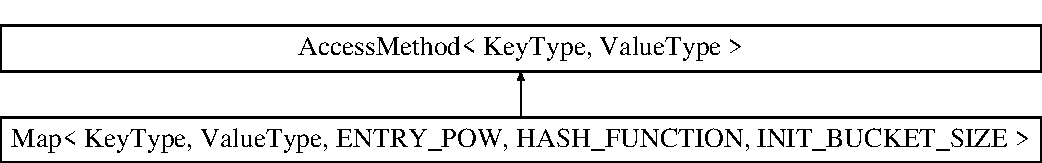
\includegraphics[height=2cm]{classMap}
\end{center}
\end{figure}
\subsection*{Classes}
\begin{CompactItemize}
\item 
struct \textbf{ENTRY\_\-}
\item 
struct \textbf{KEY\_\-}
\end{CompactItemize}
\subsection*{Public Member Functions}
\begin{CompactItemize}
\item 
\hypertarget{classMap_883205035c7253856278a8a85dc525f6}{
void \textbf{clear} ()}
\label{classMap_883205035c7253856278a8a85dc525f6}

\item 
\hypertarget{classMap_2ab48eceb4ba2747c5c7181394cfcd17}{
bool \textbf{insert} (const DataType \&data)}
\label{classMap_2ab48eceb4ba2747c5c7181394cfcd17}

\item 
\hypertarget{classMap_50367cfe4a5599c0e5d2233489288fb1}{
bool \textbf{update} (const DataType \&dat)}
\label{classMap_50367cfe4a5599c0e5d2233489288fb1}

\item 
\hypertarget{classMap_2aaa91a8937a3d449872a9f25eb3cc66}{
int \textbf{num\_\-items} () const }
\label{classMap_2aaa91a8937a3d449872a9f25eb3cc66}

\item 
\hypertarget{classMap_d422f6b43f48273263015fcf8b4e41ec}{
void \textbf{display} (std::ostream \&os=std::cout)}
\label{classMap_d422f6b43f48273263015fcf8b4e41ec}

\item 
\hypertarget{classMap_8af0b9c6da3a1fcdd954a728e9980569}{
bool \textbf{insert} (const KeyType \&key, const ValueType \&v)}
\label{classMap_8af0b9c6da3a1fcdd954a728e9980569}

\item 
\hypertarget{classMap_0d8d0efc901818fa30995ef397d333b4}{
ValueType $\ast$ \textbf{find} (const KeyType \&key)}
\label{classMap_0d8d0efc901818fa30995ef397d333b4}

\item 
\hypertarget{classMap_d22f21ff232a05b4669cae18c1485610}{
bool \textbf{del} (const KeyType \&key)}
\label{classMap_d22f21ff232a05b4669cae18c1485610}

\item 
\hypertarget{classMap_421c8a2d99d8863548d66531376fa6ef}{
bool \textbf{update} (const KeyType \&key, const ValueType \&v)}
\label{classMap_421c8a2d99d8863548d66531376fa6ef}

\item 
\hypertarget{classMap_e15503abce06dbe595275166d7eede94}{
{\footnotesize template$<$class Archive $>$ }\\void \textbf{save} (Archive \&ar, const unsigned int version) const }
\label{classMap_e15503abce06dbe595275166d7eede94}

\item 
\hypertarget{classMap_3f57005e15bc10aaf61d42097c950d91}{
{\footnotesize template$<$class Archive $>$ }\\void \textbf{load} (Archive \&ar, const unsigned int version)}
\label{classMap_3f57005e15bc10aaf61d42097c950d91}

\item 
\hypertarget{classMap_9093e5050c37e510c44ad9c8560617ad}{
void \textbf{save} (const string \&\hyperlink{classfile}{file}) const }
\label{classMap_9093e5050c37e510c44ad9c8560617ad}

\item 
\hypertarget{classMap_23c4353d14b9796736666a9d32957bf2}{
void \textbf{load} (const string \&\hyperlink{classfile}{file})}
\label{classMap_23c4353d14b9796736666a9d32957bf2}

\item 
\hypertarget{classMap_34dd2506319208393f742aabf3992ffa}{
\textbf{Map} (AllocT \&alloc, const PredT \&pred=PredT())}
\label{classMap_34dd2506319208393f742aabf3992ffa}

\item 
\hypertarget{classMap_2d90c2c5ac5feee45082e6074c90b30f}{
{\footnotesize template$<$class Iterator $>$ }\\\textbf{Map} (AllocT \&alloc, Iterator first, Iterator last, const PredT \&pred=PredT())}
\label{classMap_2d90c2c5ac5feee45082e6074c90b30f}

\item 
\hypertarget{classMap_bb40e87b15d9ce9c75cb56d83d4635f5}{
void \textbf{copy} (const Base \&from)}
\label{classMap_bb40e87b15d9ce9c75cb56d83d4635f5}

\end{CompactItemize}
\subsection*{Protected Attributes}
\begin{CompactItemize}
\item 
\hypertarget{classMap_aef62b0c834655cb9e086bea2c6f1285}{
ENTRY\_\- \textbf{entry\_\-}}
\label{classMap_aef62b0c834655cb9e086bea2c6f1285}

\item 
\hypertarget{classMap_976274497aa599402a61d4f4d062ca77}{
vector$<$ ValueType $>$ \textbf{dataVec\_\-}}
\label{classMap_976274497aa599402a61d4f4d062ca77}

\item 
\hypertarget{classMap_3bfdca718cd015a3e8ad1970e8e81cde}{
KeyType \textbf{entry\_\-size\_\-}}
\label{classMap_3bfdca718cd015a3e8ad1970e8e81cde}

\item 
\hypertarget{classMap_678a5c672b55c44e84db946081e70664}{
int \textbf{count\_\-}}
\label{classMap_678a5c672b55c44e84db946081e70664}

\end{CompactItemize}
\subsection*{Friends}
\begin{CompactItemize}
\item 
\hypertarget{classMap_c98d07dd8f7b70e16ccb9a01abf56b9c}{
class \textbf{boost::serialization::access}}
\label{classMap_c98d07dd8f7b70e16ccb9a01abf56b9c}

\end{CompactItemize}


\subsection{Detailed Description}
\subsubsection*{template$<$class KeyType = uint32\_\-t, class ValueType = uint64\_\-t, size\_\-t ENTRY\_\-POW = 16, class HASH\_\-FUNCTION = simple\_\-hash, int INIT\_\-BUCKET\_\-SIZE = 64$>$ class Map$<$ KeyType, ValueType, ENTRY\_\-POW, HASH\_\-FUNCTION, INIT\_\-BUCKET\_\-SIZE $>$}

This is an implementation of open addressing and linear probing hash table for integer key. 

Definition at line 65 of file map.hpp.

The documentation for this class was generated from the following files:\begin{CompactItemize}
\item 
/home/Kevin/izenelib/include/am/map/map.hpp\item 
/home/Kevin/izenelib/include/util/Map.h\end{CompactItemize}

\hypertarget{classrequest}{
\section{request Class Reference}
\label{classrequest}\index{request@{request}}
}
Defines interface of \hyperlink{classrequest}{request}.  


{\tt \#include $<$iobase.h$>$}

Inheritance diagram for request::\begin{figure}[H]
\begin{center}
\leavevmode
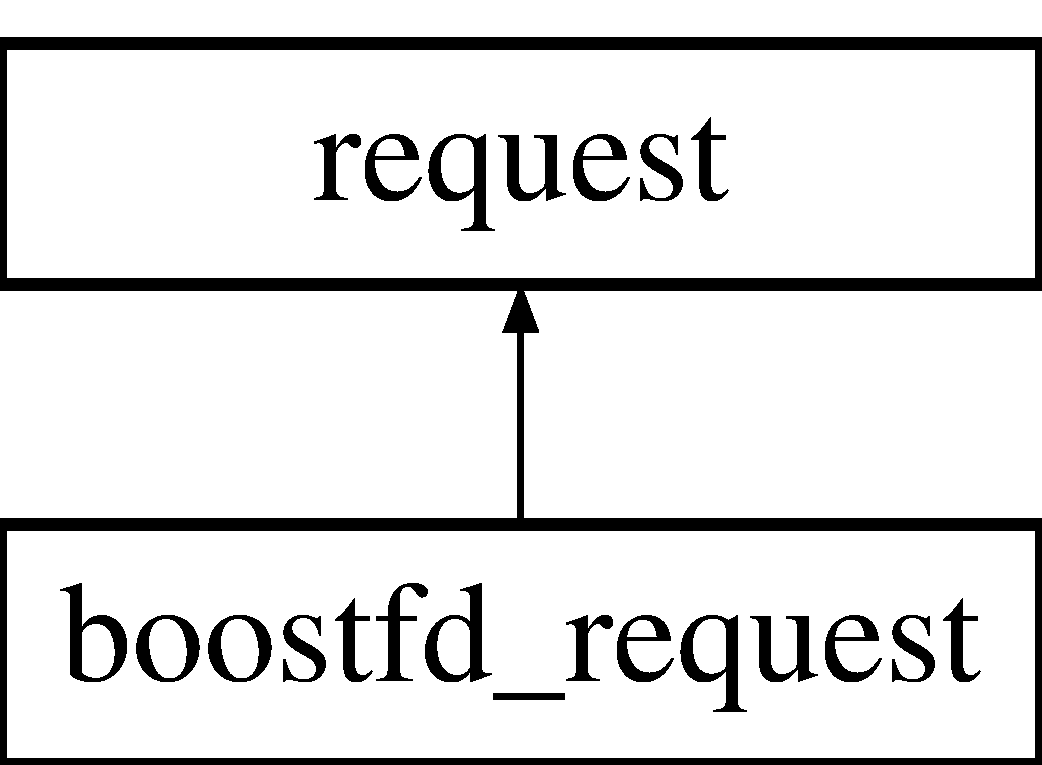
\includegraphics[height=2cm]{classrequest}
\end{center}
\end{figure}
\subsection*{Public Types}
\begin{CompactItemize}
\item 
enum \textbf{request\_\-type} \{ \textbf{READ}, 
\textbf{WRITE}
 \}
\end{CompactItemize}
\subsection*{Public Member Functions}
\begin{CompactItemize}
\item 
\hypertarget{group__iolayer_g31f7e409bd2e9ade994975b3752f33d1}{
\textbf{request} (\hyperlink{classcompletion__handler}{completion\_\-handler} on\_\-compl, \hyperlink{classfile}{file} $\ast$file\_\-\_\-, void $\ast$buffer\_\-, int64\_\-t offset\_\-, size\_\-t bytes\_\-, request\_\-type type\_\-)}
\label{group__iolayer_g31f7e409bd2e9ade994975b3752f33d1}

\item 
\hypertarget{group__iolayer_g2cdb5763d21b553ae816eb4152e5d89b}{
virtual void \hyperlink{group__iolayer_g2cdb5763d21b553ae816eb4152e5d89b}{wait} ()=0}
\label{group__iolayer_g2cdb5763d21b553ae816eb4152e5d89b}

\begin{CompactList}\small\item\em Suspends calling thread until completion of the \hyperlink{classrequest}{request}. \item\end{CompactList}\item 
virtual bool \hyperlink{group__iolayer_ge93809a6f19558a9f0f98f50cd69aa2f}{poll} ()=0
\begin{CompactList}\small\item\em Polls the status of the \hyperlink{classrequest}{request}. \item\end{CompactList}\item 
\hypertarget{group__iolayer_g1791fb9aa3161faec8b1660e01525e26}{
\hyperlink{classfile}{file} $\ast$ \textbf{get\_\-file} () const }
\label{group__iolayer_g1791fb9aa3161faec8b1660e01525e26}

\item 
\hypertarget{group__iolayer_gbc0add4ffc5e7c696ed4067cf630d935}{
void $\ast$ \textbf{get\_\-buffer} () const }
\label{group__iolayer_gbc0add4ffc5e7c696ed4067cf630d935}

\item 
\hypertarget{group__iolayer_gd8cb0dcaea77815e50f9d9f55b84db27}{
int64\_\-t \textbf{get\_\-offset} () const }
\label{group__iolayer_gd8cb0dcaea77815e50f9d9f55b84db27}

\item 
\hypertarget{group__iolayer_ge19716d99090239ece78660b0c7d567f}{
size\_\-t \textbf{get\_\-size} () const }
\label{group__iolayer_ge19716d99090239ece78660b0c7d567f}

\item 
\hypertarget{group__iolayer_g9bc852dd0ab2900911465f6a8e03ca6e}{
size\_\-t \textbf{size} () const }
\label{group__iolayer_g9bc852dd0ab2900911465f6a8e03ca6e}

\item 
\hypertarget{group__iolayer_gca7a3651bcfab4842a426399756b47e1}{
request\_\-type \textbf{get\_\-type} () const }
\label{group__iolayer_gca7a3651bcfab4842a426399756b47e1}

\item 
\hypertarget{group__iolayer_gbc1ade28e4e71c83eb166af89898350c}{
virtual std::ostream \& \textbf{print} (std::ostream \&out) const }
\label{group__iolayer_gbc1ade28e4e71c83eb166af89898350c}

\item 
\hypertarget{group__iolayer_gf946fd2411a5b613d195bc46c914facc}{
void \hyperlink{group__iolayer_gf946fd2411a5b613d195bc46c914facc}{error\_\-occured} (const char $\ast$msg)}
\label{group__iolayer_gf946fd2411a5b613d195bc46c914facc}

\begin{CompactList}\small\item\em Inform the \hyperlink{classrequest}{request} object that an error occurred during the I/O execution. \item\end{CompactList}\item 
\hypertarget{group__iolayer_g8bfe152a78eb167f7a07f573614c07b6}{
void \hyperlink{group__iolayer_g8bfe152a78eb167f7a07f573614c07b6}{error\_\-occured} (const std::string \&msg)}
\label{group__iolayer_g8bfe152a78eb167f7a07f573614c07b6}

\begin{CompactList}\small\item\em Inform the \hyperlink{classrequest}{request} object that an error occurred during the I/O execution. \item\end{CompactList}\item 
\hypertarget{group__iolayer_g32dc55876ffe5160f8c037b3c6eaf126}{
void \hyperlink{group__iolayer_g32dc55876ffe5160f8c037b3c6eaf126}{check\_\-errors} ()  throw (std::ios\_\-base::failure)}
\label{group__iolayer_g32dc55876ffe5160f8c037b3c6eaf126}

\begin{CompactList}\small\item\em Rises an exception if there were error with the I/O. \item\end{CompactList}\end{CompactItemize}
\subsection*{Protected Member Functions}
\begin{CompactItemize}
\item 
\hypertarget{group__iolayer_g2f72232aa958b26b36b04c2ade02b1d6}{
virtual bool \textbf{add\_\-waiter} (onoff\_\-switch $\ast$sw)=0}
\label{group__iolayer_g2f72232aa958b26b36b04c2ade02b1d6}

\item 
\hypertarget{group__iolayer_g30252a01456b49135c054dde2b8e8c6d}{
virtual void \textbf{delete\_\-waiter} (onoff\_\-switch $\ast$sw)=0}
\label{group__iolayer_g30252a01456b49135c054dde2b8e8c6d}

\item 
\hypertarget{group__iolayer_g47a70e642437bd2a3cdcb2f64e269fcb}{
virtual void \textbf{serve} ()=0}
\label{group__iolayer_g47a70e642437bd2a3cdcb2f64e269fcb}

\item 
\hypertarget{group__iolayer_gdae52da05a69bea331d1161156159b06}{
void \textbf{completed} ()}
\label{group__iolayer_gdae52da05a69bea331d1161156159b06}

\item 
\hypertarget{group__iolayer_g11bad6558be8c299ed7c14f0ed9e62d2}{
int \textbf{nref} ()}
\label{group__iolayer_g11bad6558be8c299ed7c14f0ed9e62d2}

\end{CompactItemize}
\subsection*{Protected Attributes}
\begin{CompactItemize}
\item 
\hypertarget{group__iolayer_g2d9258e3443b499e4c641c2843bdc7a1}{
\hyperlink{classcompletion__handler}{completion\_\-handler} \textbf{on\_\-complete}}
\label{group__iolayer_g2d9258e3443b499e4c641c2843bdc7a1}

\item 
\hypertarget{group__iolayer_gbc00c1450db214bd32b3936d95730401}{
int \textbf{ref\_\-cnt}}
\label{group__iolayer_gbc00c1450db214bd32b3936d95730401}

\item 
\hypertarget{group__iolayer_g8f916a380f56a5017fdb196f76feaf31}{
std::auto\_\-ptr$<$ std::ios\_\-base::failure $>$ \textbf{error}}
\label{group__iolayer_g8f916a380f56a5017fdb196f76feaf31}

\item 
\hypertarget{group__iolayer_g341cdc5f009668b88edc9415720c6bc0}{
boost::mutex \textbf{ref\_\-cnt\_\-mutex}}
\label{group__iolayer_g341cdc5f009668b88edc9415720c6bc0}

\item 
\hypertarget{group__iolayer_gf25e69a9ec49b9aeb592ff28b9a1697e}{
\hyperlink{classfile}{file} $\ast$ \textbf{file\_\-}}
\label{group__iolayer_gf25e69a9ec49b9aeb592ff28b9a1697e}

\item 
\hypertarget{group__iolayer_g073eb2eba36110cc4362765aba803cdd}{
void $\ast$ \textbf{buffer}}
\label{group__iolayer_g073eb2eba36110cc4362765aba803cdd}

\item 
\hypertarget{group__iolayer_gbfc7b5f60fb16d3551e21fbba49d75dc}{
int64\_\-t \textbf{offset}}
\label{group__iolayer_gbfc7b5f60fb16d3551e21fbba49d75dc}

\item 
\hypertarget{group__iolayer_gffe23f8f72bfd5e016c3c7125740f96b}{
size\_\-t \textbf{bytes}}
\label{group__iolayer_gffe23f8f72bfd5e016c3c7125740f96b}

\item 
\hypertarget{group__iolayer_gcc85c654247d6d16afb0b1d63a7d3c8e}{
request\_\-type \textbf{type}}
\label{group__iolayer_gcc85c654247d6d16afb0b1d63a7d3c8e}

\end{CompactItemize}
\subsection*{Friends}
\begin{CompactItemize}
\item 
\hypertarget{group__iolayer_g686a90482e62dd1618201a3c79f9aae6}{
class \hyperlink{group__iolayer_g686a90482e62dd1618201a3c79f9aae6}{file}}
\label{group__iolayer_g686a90482e62dd1618201a3c79f9aae6}

\item 
\hypertarget{group__iolayer_g04639cad0832bf1448ee1bb4976a05c9}{
class \textbf{disk\_\-queue}}
\label{group__iolayer_g04639cad0832bf1448ee1bb4976a05c9}

\item 
\hypertarget{group__iolayer_g41c8636643792c137da130157a9ca431}{
class \hyperlink{group__iolayer_g41c8636643792c137da130157a9ca431}{request\_\-ptr}}
\label{group__iolayer_g41c8636643792c137da130157a9ca431}

\item 
int \hyperlink{classrequest_7a455713cd840b099075368af3f30ff5}{wait\_\-any} (\hyperlink{classrequest__ptr}{request\_\-ptr} req\_\-array\mbox{[}$\,$\mbox{]}, int count)
\begin{CompactList}\small\item\em Collection of functions to track statuses of a number of requests. \item\end{CompactList}\item 
\hypertarget{group__iolayer_g2bfbfc0bc801311fd2933969ca786fef}{
{\footnotesize template$<$class request\_\-iterator\_\- $>$ }\\request\_\-iterator\_\- \textbf{wait\_\-any} (request\_\-iterator\_\- reqs\_\-begin, request\_\-iterator\_\- reqs\_\-end)}
\label{group__iolayer_g2bfbfc0bc801311fd2933969ca786fef}

\end{CompactItemize}


\subsection{Detailed Description}
Defines interface of \hyperlink{classrequest}{request}. 

Since all library I/O operations are asynchronous, one needs to keep track of their status: whether an I/O completed or not. 

Definition at line 179 of file iobase.h.

\subsection{Friends And Related Function Documentation}
\hypertarget{classrequest_7a455713cd840b099075368af3f30ff5}{
\index{request@{request}!wait\_\-any@{wait\_\-any}}
\index{wait\_\-any@{wait\_\-any}!request@{request}}
\subsubsection[{wait\_\-any}]{\setlength{\rightskip}{0pt plus 5cm}int wait\_\-any ({\bf request\_\-ptr} {\em req\_\-array}\mbox{[}$\,$\mbox{]}, \/  int {\em count})\hspace{0.3cm}{\tt  \mbox{[}friend\mbox{]}}}}
\label{classrequest_7a455713cd840b099075368af3f30ff5}


Collection of functions to track statuses of a number of requests. 

Suspends calling thread until {\bf any} of requests is completed \begin{Desc}
\item[Parameters:]
\begin{description}
\item[{\em req\_\-array}]array of {\tt \hyperlink{classrequest__ptr}{request\_\-ptr}} objects \item[{\em count}]size of req\_\-array \end{description}
\end{Desc}
\begin{Desc}
\item[Returns:]index in req\_\-array pointing to the {\bf first} completed \hyperlink{classrequest}{request} \end{Desc}


The documentation for this class was generated from the following file:\begin{CompactItemize}
\item 
/home/Kevin/izenelib/include/am/blockmanager/iobase.h\end{CompactItemize}

\hypertarget{classrequest__ptr}{
\section{request\_\-ptr Class Reference}
\label{classrequest__ptr}\index{request\_\-ptr@{request\_\-ptr}}
}
A smart wrapper for {\tt \hyperlink{classrequest}{request}} pointer.  


{\tt \#include $<$iobase.h$>$}

\subsection*{Public Member Functions}
\begin{CompactItemize}
\item 
\hypertarget{group__iolayer_ge78ff55c792061dae60eebda7b08615a}{
\hyperlink{group__iolayer_ge78ff55c792061dae60eebda7b08615a}{request\_\-ptr} (\hyperlink{classrequest}{request} $\ast$ptr\_\-=NULL)}
\label{group__iolayer_ge78ff55c792061dae60eebda7b08615a}

\begin{CompactList}\small\item\em Constructs an {\tt \hyperlink{classrequest__ptr}{request\_\-ptr}} from {\tt \hyperlink{classrequest}{request}} pointer. \item\end{CompactList}\item 
\hypertarget{group__iolayer_gfbd62f3bb0fe9378ffe9defd6be764dc}{
\hyperlink{group__iolayer_gfbd62f3bb0fe9378ffe9defd6be764dc}{request\_\-ptr} (const \hyperlink{classrequest__ptr}{request\_\-ptr} \&p)}
\label{group__iolayer_gfbd62f3bb0fe9378ffe9defd6be764dc}

\begin{CompactList}\small\item\em Constructs an {\tt \hyperlink{classrequest__ptr}{request\_\-ptr}} from a {\tt \hyperlink{classrequest__ptr}{request\_\-ptr}} object. \item\end{CompactList}\item 
\hypertarget{group__iolayer_g3dd322205e1e61403b2d14874a543ab4}{
\hyperlink{group__iolayer_g3dd322205e1e61403b2d14874a543ab4}{$\sim$request\_\-ptr} ()}
\label{group__iolayer_g3dd322205e1e61403b2d14874a543ab4}

\begin{CompactList}\small\item\em Destructor. \item\end{CompactList}\item 
\hyperlink{classrequest__ptr}{request\_\-ptr} \& \hyperlink{group__iolayer_g1f361f479f69ffb179ec4b54615aa1b5}{operator=} (const \hyperlink{classrequest__ptr}{request\_\-ptr} \&p)
\begin{CompactList}\small\item\em Assignment operator from {\tt \hyperlink{classrequest__ptr}{request\_\-ptr}} object. \item\end{CompactList}\item 
\hyperlink{classrequest__ptr}{request\_\-ptr} \& \hyperlink{group__iolayer_gfef634a7f244626b88ccfb71f93060e8}{operator=} (\hyperlink{classrequest}{request} $\ast$p)
\begin{CompactList}\small\item\em Assignment operator from {\tt \hyperlink{classrequest}{request}} pointer. \item\end{CompactList}\item 
\hyperlink{classrequest}{request} \& \hyperlink{group__iolayer_g15bd551f80acd18f2d0e3a1aade2b40c}{operator$\ast$} () const 
\begin{CompactList}\small\item\em \char`\"{}Star\char`\"{} operator \item\end{CompactList}\item 
\hyperlink{classrequest}{request} $\ast$ \hyperlink{group__iolayer_g9ccc7167eaa30948950571a094b9c902}{operator $\rightarrow$ } () const 
\begin{CompactList}\small\item\em \char`\"{}Arrow\char`\"{} operator \item\end{CompactList}\item 
\hyperlink{classrequest}{request} $\ast$ \hyperlink{group__iolayer_g30490f3d014bae40a66022640fb34153}{get} () const 
\begin{CompactList}\small\item\em Access to owned {\tt \hyperlink{classrequest}{request}} object (synonym for {\tt \hyperlink{group__iolayer_g9ccc7167eaa30948950571a094b9c902}{operator $\rightarrow$ ()}} ). \item\end{CompactList}\item 
\hypertarget{group__iolayer_g848a2fc2a409c2d22bd8a91dd22aebba}{
bool \hyperlink{group__iolayer_g848a2fc2a409c2d22bd8a91dd22aebba}{valid} () const }
\label{group__iolayer_g848a2fc2a409c2d22bd8a91dd22aebba}

\begin{CompactList}\small\item\em Returns true if object is initialized. \item\end{CompactList}\item 
\hypertarget{group__iolayer_g41b7141c1c672fac687ab81ce5438017}{
bool \hyperlink{group__iolayer_g41b7141c1c672fac687ab81ce5438017}{empty} () const }
\label{group__iolayer_g41b7141c1c672fac687ab81ce5438017}

\begin{CompactList}\small\item\em Returns true if object is not initialized. \item\end{CompactList}\end{CompactItemize}


\subsection{Detailed Description}
A smart wrapper for {\tt \hyperlink{classrequest}{request}} pointer. 

Implemented as reference counting smart pointer. 

Definition at line 326 of file iobase.h.

The documentation for this class was generated from the following file:\begin{CompactItemize}
\item 
/home/Kevin/izenelib/include/am/blockmanager/iobase.h\end{CompactItemize}

\hypertarget{classsdb__btree}{
\section{sdb\_\-btree$<$ KeyType, ValueType, LockType, Alloc $>$ Class Template Reference}
\label{classsdb__btree}\index{sdb\_\-btree@{sdb\_\-btree}}
}
\hyperlink{classfile}{file} version of cc-b$\ast$-btree  


{\tt \#include $<$sdb\_\-btree.h$>$}

Inheritance diagram for sdb\_\-btree$<$ KeyType, ValueType, LockType, Alloc $>$::\begin{figure}[H]
\begin{center}
\leavevmode
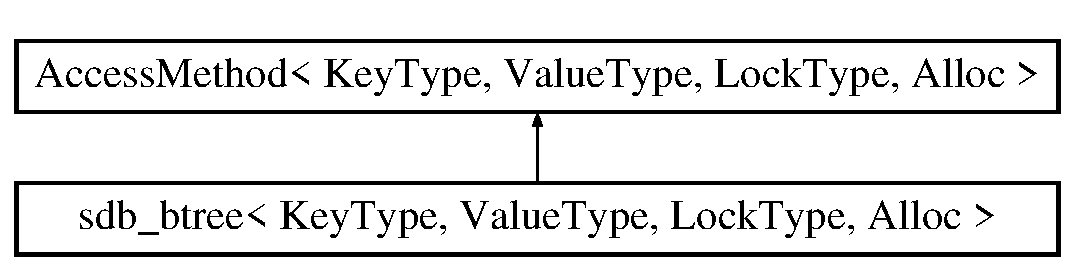
\includegraphics[height=2cm]{classsdb__btree}
\end{center}
\end{figure}
\subsection*{Public Types}
\begin{CompactItemize}
\item 
\hypertarget{classsdb__btree_15a24f87a9a407de8b68ee054af3b54a}{
typedef sdb\_\-node\_\-$<$ KeyType, ValueType, LockType, Alloc $>$ \textbf{sdb\_\-node}}
\label{classsdb__btree_15a24f87a9a407de8b68ee054af3b54a}

\item 
\hypertarget{classsdb__btree_d6105a305901616127f769f0147a5e03}{
typedef DataType$<$ KeyType, ValueType $>$ \textbf{DataType}}
\label{classsdb__btree_d6105a305901616127f769f0147a5e03}

\item 
\hypertarget{classsdb__btree_6c8e77fb4c105a87903d11cb6b28f62c}{
typedef std::pair$<$ sdb\_\-node $\ast$, size\_\-t $>$ \textbf{SDBCursor}}
\label{classsdb__btree_6c8e77fb4c105a87903d11cb6b28f62c}

\end{CompactItemize}
\subsection*{Public Member Functions}
\begin{CompactItemize}
\item 
\hyperlink{classsdb__btree_ae55c86e49f1ff7c02f4251ccfe8c625}{sdb\_\-btree} (const std::string \&fileName=\char`\"{}sequentialdb.dat\#\char`\"{})
\begin{CompactList}\small\item\em constructor \item\end{CompactList}\item 
void \hyperlink{classsdb__btree_1f6eb93d26b290d3969de6503672ae07}{setBtreeMode} (bool delaySplit)
\begin{CompactList}\small\item\em set mod \item\end{CompactList}\item 
void \hyperlink{classsdb__btree_c393399c9c8b9a1f06ecb4f4cce15bf0}{setMaxKeys} (size\_\-t maxkeys)
\begin{CompactList}\small\item\em set the MaxKeys \item\end{CompactList}\item 
void \hyperlink{classsdb__btree_fc9d66b5f80ba33b114c5f4db70a8dc6}{setDegree} (size\_\-t degree)
\begin{CompactList}\small\item\em set maxKeys for fileHeader \item\end{CompactList}\item 
void \hyperlink{classsdb__btree_930cde276bf7ed268a7005ba92dfbf12}{setPageSize} (size\_\-t pageSize)
\begin{CompactList}\small\item\em set tha pageSize of fileHeader. \item\end{CompactList}\item 
void \hyperlink{classsdb__btree_a815f13cd8a7cf18a93190e6aa9c4efc}{setCacheSize} (size\_\-t sz)
\begin{CompactList}\small\item\em set Cache Size. \item\end{CompactList}\item 
\hypertarget{classsdb__btree_85f5043da06823365665619cda9eebb2}{
std::string \hyperlink{classsdb__btree_85f5043da06823365665619cda9eebb2}{getFileName} () const }
\label{classsdb__btree_85f5043da06823365665619cda9eebb2}

\begin{CompactList}\small\item\em return the \hyperlink{classfile}{file} name of the SequentialDB \item\end{CompactList}\item 
bool \hyperlink{classsdb__btree_3930f68c0075a965d79dae75586e611d}{open} ()
\begin{CompactList}\small\item\em open the database. \item\end{CompactList}\item 
bool \hyperlink{classsdb__btree_2da914c45fec1081667fb22d42a021a5}{close} ()
\begin{CompactList}\small\item\em close the database. \item\end{CompactList}\item 
\hypertarget{classsdb__btree_30e2c2e7489f8785c86284e09b75bcfb}{
bool \hyperlink{classsdb__btree_30e2c2e7489f8785c86284e09b75bcfb}{del} (const KeyType \&key)}
\label{classsdb__btree_30e2c2e7489f8785c86284e09b75bcfb}

\begin{CompactList}\small\item\em del an item from the database \item\end{CompactList}\item 
\hypertarget{classsdb__btree_3f3988638bc90b19230f5c80dd960dad}{
bool \hyperlink{classsdb__btree_3f3988638bc90b19230f5c80dd960dad}{insert} (const DataType \&rec)}
\label{classsdb__btree_3f3988638bc90b19230f5c80dd960dad}

\begin{CompactList}\small\item\em insert an item. \item\end{CompactList}\item 
\hypertarget{classsdb__btree_1bc062c093b1b5599313bcf33af0820f}{
bool \hyperlink{classsdb__btree_1bc062c093b1b5599313bcf33af0820f}{insert} (const KeyType \&key, const ValueType \&value)}
\label{classsdb__btree_1bc062c093b1b5599313bcf33af0820f}

\begin{CompactList}\small\item\em insert an item. \item\end{CompactList}\item 
\hypertarget{classsdb__btree_42fb2964951af3294e544f857f23349b}{
ValueType $\ast$ \hyperlink{classsdb__btree_42fb2964951af3294e544f857f23349b}{find} (const KeyType \&key)}
\label{classsdb__btree_42fb2964951af3294e544f857f23349b}

\begin{CompactList}\small\item\em find an item given a key. \item\end{CompactList}\item 
\hypertarget{classsdb__btree_1fe7be112c01719109bf98f803777417}{
bool \textbf{get} (const KeyType \&key, ValueType \&value)}
\label{classsdb__btree_1fe7be112c01719109bf98f803777417}

\item 
\hypertarget{classsdb__btree_a4d71e716f6c61ff4f1f78317dcc9a17}{
const ValueType $\ast$ \hyperlink{classsdb__btree_a4d71e716f6c61ff4f1f78317dcc9a17}{find} (const KeyType \&key) const }
\label{classsdb__btree_a4d71e716f6c61ff4f1f78317dcc9a17}

\begin{CompactList}\small\item\em find an item given a key. \item\end{CompactList}\item 
\hypertarget{classsdb__btree_cb2ca67cdc1d405212cfd2332b626cda}{
bool \hyperlink{classsdb__btree_cb2ca67cdc1d405212cfd2332b626cda}{update} (const KeyType \&key, const ValueType \&val)}
\label{classsdb__btree_cb2ca67cdc1d405212cfd2332b626cda}

\begin{CompactList}\small\item\em updata an item with given key, if it not exist, insert it directly. \item\end{CompactList}\item 
\hypertarget{classsdb__btree_e0bab2b948984fcaae6d38f161fad06f}{
bool \hyperlink{classsdb__btree_e0bab2b948984fcaae6d38f161fad06f}{update} (const DataType \&rec)}
\label{classsdb__btree_e0bab2b948984fcaae6d38f161fad06f}

\begin{CompactList}\small\item\em updata an item with given key, if it not exist, insert it directly. \item\end{CompactList}\item 
\hypertarget{classsdb__btree_4c3e3043ff613cb1f81d6c7d60279562}{
int \hyperlink{classsdb__btree_4c3e3043ff613cb1f81d6c7d60279562}{num\_\-items} ()}
\label{classsdb__btree_4c3e3043ff613cb1f81d6c7d60279562}

\begin{CompactList}\small\item\em get the number of the items. \item\end{CompactList}\item 
\hypertarget{classsdb__btree_4796b30a0a456d6ff6f3c395f9a2647f}{
bool \hyperlink{classsdb__btree_4796b30a0a456d6ff6f3c395f9a2647f}{get} (const SDBCursor \&locn, DataType \&rec)}
\label{classsdb__btree_4796b30a0a456d6ff6f3c395f9a2647f}

\begin{CompactList}\small\item\em get an item from given Locn. $\ast$ \item\end{CompactList}\item 
\hypertarget{classsdb__btree_4e4408d7daafd2fcf1a1baeff8101765}{
bool \hyperlink{classsdb__btree_4e4408d7daafd2fcf1a1baeff8101765}{get} (const SDBCursor \&locn, KeyType \&key, ValueType \&value)}
\label{classsdb__btree_4e4408d7daafd2fcf1a1baeff8101765}

\begin{CompactList}\small\item\em get an item from given Locn. $\ast$ \item\end{CompactList}\item 
\hypertarget{classsdb__btree_0388b79df1693137217f884588e2e30d}{
SDBCursor \hyperlink{classsdb__btree_0388b79df1693137217f884588e2e30d}{get\_\-first\_\-locn} ()}
\label{classsdb__btree_0388b79df1693137217f884588e2e30d}

\begin{CompactList}\small\item\em get the cursor of the first item. \item\end{CompactList}\item 
bool \hyperlink{classsdb__btree_dfcd196457bcb4517403a6471a7076af}{seq} (SDBCursor \&locn, DataType \&rec, ESeqDirection sdir=ESD\_\-FORWARD)
\begin{CompactList}\small\item\em get the next or prev item. \item\end{CompactList}\item 
\hypertarget{classsdb__btree_1e6e4ead81ba7d871919a601fd68c1e6}{
void \hyperlink{classsdb__btree_1e6e4ead81ba7d871919a601fd68c1e6}{flush} ()}
\label{classsdb__btree_1e6e4ead81ba7d871919a601fd68c1e6}

\begin{CompactList}\small\item\em write all the items in memory to \hyperlink{classfile}{file}. \item\end{CompactList}\item 
\hypertarget{classsdb__btree_4336e972867ad749ce98519fe5220bc5}{
void \hyperlink{classsdb__btree_4336e972867ad749ce98519fe5220bc5}{commit} ()}
\label{classsdb__btree_4336e972867ad749ce98519fe5220bc5}

\begin{CompactList}\small\item\em write back the dirypages \item\end{CompactList}\item 
void \hyperlink{classsdb__btree_b1f5ad2d92b57af57aca4a06c925bb16}{display} (std::ostream \&os=std::cout, bool onlyheader=true)
\item 
\hypertarget{classsdb__btree_cc591b9dee49543d1a39891f4af1b842}{
SDBCursor \hyperlink{classsdb__btree_cc591b9dee49543d1a39891f4af1b842}{search} (const KeyType \&key)}
\label{classsdb__btree_cc591b9dee49543d1a39891f4af1b842}

\begin{CompactList}\small\item\em Get the DB cursor of given key. \item\end{CompactList}\item 
bool \hyperlink{classsdb__btree_2761e4efefbe470ca5121c2eb19f6a6e}{search} (const KeyType \&key, SDBCursor \&locn)
\begin{CompactList}\small\item\em get the cursor for given key \item\end{CompactList}\end{CompactItemize}


\subsection{Detailed Description}
\subsubsection*{template$<$typename KeyType, typename ValueType = NullType, typename LockType = NullLock, typename Alloc = std::allocator$<$DataType$<$KeyType,ValueType$>$ $>$$>$ class sdb\_\-btree$<$ KeyType, ValueType, LockType, Alloc $>$}

\hyperlink{classfile}{file} version of cc-b$\ast$-btree 

A B$\ast$-tree is a tree data structure used in the HFS and Reiser4 \hyperlink{classfile}{file} systems, which requires non-root nodes to be at least 2/3 full instead of 1/2. To maintain this, instead of immediately splitting up a node when it gets full, its keys are shared with the node next to it. When both are full, then the two of them are split into three. Now SDBv1.0’s disk space is large than BerkeleyDB when storing the same data set. There is a perspective that, B$\ast$-tree can save more disk space than normal btree.

For implementation convience and maintainess, we only apply this delay splitting at leaves nodes.

Merging will occur when two sibling nodes' objCount both less than maxKeys/3/ 

Definition at line 42 of file sdb\_\-btree.h.

\subsection{Constructor \& Destructor Documentation}
\hypertarget{classsdb__btree_ae55c86e49f1ff7c02f4251ccfe8c625}{
\index{sdb\_\-btree@{sdb\_\-btree}!sdb\_\-btree@{sdb\_\-btree}}
\index{sdb\_\-btree@{sdb\_\-btree}!sdb_btree@{sdb\_\-btree}}
\subsubsection[{sdb\_\-btree}]{\setlength{\rightskip}{0pt plus 5cm}template$<$typename KeyType , typename ValueType , typename LockType , typename Alloc $>$ {\bf sdb\_\-btree}$<$ KeyType, ValueType, LockType, Alloc $>$::{\bf sdb\_\-btree} (const std::string \& {\em fileName} = {\tt \char`\"{}sequentialdb.dat\#\char`\"{}})\hspace{0.3cm}{\tt  \mbox{[}inline\mbox{]}}}}
\label{classsdb__btree_ae55c86e49f1ff7c02f4251ccfe8c625}


constructor 

\begin{Desc}
\item[Parameters:]
\begin{description}
\item[{\em fileName}]is the name for data \hyperlink{classfile}{file} if fileName ends with '\#', we set b-tree mode to not delay split. \end{description}
\end{Desc}


Definition at line 493 of file sdb\_\-btree.h.

\subsection{Member Function Documentation}
\hypertarget{classsdb__btree_2da914c45fec1081667fb22d42a021a5}{
\index{sdb\_\-btree@{sdb\_\-btree}!close@{close}}
\index{close@{close}!sdb_btree@{sdb\_\-btree}}
\subsubsection[{close}]{\setlength{\rightskip}{0pt plus 5cm}template$<$typename KeyType , typename ValueType  = NullType, typename LockType  = NullLock, typename Alloc  = std::allocator$<$DataType$<$KeyType,ValueType$>$ $>$$>$ bool {\bf sdb\_\-btree}$<$ KeyType, ValueType, LockType, Alloc $>$::close ()\hspace{0.3cm}{\tt  \mbox{[}inline\mbox{]}}}}
\label{classsdb__btree_2da914c45fec1081667fb22d42a021a5}


close the database. 

if we don't call it, it will be automately called in deconstructor 

Definition at line 160 of file sdb\_\-btree.h.\hypertarget{classsdb__btree_b1f5ad2d92b57af57aca4a06c925bb16}{
\index{sdb\_\-btree@{sdb\_\-btree}!display@{display}}
\index{display@{display}!sdb_btree@{sdb\_\-btree}}
\subsubsection[{display}]{\setlength{\rightskip}{0pt plus 5cm}template$<$typename KeyType , typename ValueType  = NullType, typename LockType  = NullLock, typename Alloc  = std::allocator$<$DataType$<$KeyType,ValueType$>$ $>$$>$ void {\bf sdb\_\-btree}$<$ KeyType, ValueType, LockType, Alloc $>$::display (std::ostream \& {\em os} = {\tt std::cout}, \/  bool {\em onlyheader} = {\tt true})\hspace{0.3cm}{\tt  \mbox{[}inline\mbox{]}}}}
\label{classsdb__btree_b1f5ad2d92b57af57aca4a06c925bb16}


for debug. print the shape of the B tree. 

Definition at line 317 of file sdb\_\-btree.h.\hypertarget{classsdb__btree_3930f68c0075a965d79dae75586e611d}{
\index{sdb\_\-btree@{sdb\_\-btree}!open@{open}}
\index{open@{open}!sdb_btree@{sdb\_\-btree}}
\subsubsection[{open}]{\setlength{\rightskip}{0pt plus 5cm}template$<$typename KeyType , typename ValueType , typename LockType , typename Alloc $>$ bool {\bf sdb\_\-btree}$<$ KeyType, ValueType, LockType, Alloc $>$::open ()\hspace{0.3cm}{\tt  \mbox{[}inline\mbox{]}}}}
\label{classsdb__btree_3930f68c0075a965d79dae75586e611d}


open the database. 

Everytime we use the database, we mush open it first. 

Definition at line 1237 of file sdb\_\-btree.h.\hypertarget{classsdb__btree_2761e4efefbe470ca5121c2eb19f6a6e}{
\index{sdb\_\-btree@{sdb\_\-btree}!search@{search}}
\index{search@{search}!sdb_btree@{sdb\_\-btree}}
\subsubsection[{search}]{\setlength{\rightskip}{0pt plus 5cm}template$<$typename KeyType , typename ValueType , typename LockType , typename Alloc $>$ bool {\bf sdb\_\-btree}$<$ KeyType, ValueType, LockType, Alloc $>$::search (const KeyType \& {\em key}, \/  SDBCursor \& {\em locn})\hspace{0.3cm}{\tt  \mbox{[}inline\mbox{]}}}}
\label{classsdb__btree_2761e4efefbe470ca5121c2eb19f6a6e}


get the cursor for given key 

\begin{Desc}
\item[Parameters:]
\begin{description}
\item[{\em locn}]is cursor of key. \end{description}
\end{Desc}
\begin{Desc}
\item[Returns:]true if key exists otherwise false. \end{Desc}


Definition at line 516 of file sdb\_\-btree.h.\hypertarget{classsdb__btree_dfcd196457bcb4517403a6471a7076af}{
\index{sdb\_\-btree@{sdb\_\-btree}!seq@{seq}}
\index{seq@{seq}!sdb_btree@{sdb\_\-btree}}
\subsubsection[{seq}]{\setlength{\rightskip}{0pt plus 5cm}template$<$typename KeyType , typename ValueType , typename LockType , typename Alloc $>$ bool {\bf sdb\_\-btree}$<$ KeyType, ValueType, LockType, Alloc $>$::seq (SDBCursor \& {\em locn}, \/  DataType \& {\em rec}, \/  ESeqDirection {\em sdir} = {\tt ESD\_\-FORWARD})\hspace{0.3cm}{\tt  \mbox{[}inline\mbox{]}}}}
\label{classsdb__btree_dfcd196457bcb4517403a6471a7076af}


get the next or prev item. 

when locn is default value, it will start with firt element when sdri=ESD\_\-FORWARD and start with last element when sdir = ESD\_\-BACKWARD 

Definition at line 1372 of file sdb\_\-btree.h.\hypertarget{classsdb__btree_1f6eb93d26b290d3969de6503672ae07}{
\index{sdb\_\-btree@{sdb\_\-btree}!setBtreeMode@{setBtreeMode}}
\index{setBtreeMode@{setBtreeMode}!sdb_btree@{sdb\_\-btree}}
\subsubsection[{setBtreeMode}]{\setlength{\rightskip}{0pt plus 5cm}template$<$typename KeyType , typename ValueType  = NullType, typename LockType  = NullLock, typename Alloc  = std::allocator$<$DataType$<$KeyType,ValueType$>$ $>$$>$ void {\bf sdb\_\-btree}$<$ KeyType, ValueType, LockType, Alloc $>$::setBtreeMode (bool {\em delaySplit})\hspace{0.3cm}{\tt  \mbox{[}inline\mbox{]}}}}
\label{classsdb__btree_1f6eb93d26b290d3969de6503672ae07}


set mod 

\begin{Desc}
\item[Parameters:]
\begin{description}
\item[{\em delaySplit,if}]true, the btree is cc-b$\ast$-btee, otherwise is normal cc-b-tree.\end{description}
\end{Desc}
For ascending insertion, cc-b-tree is much faster than cc-b$\ast$-btree, while cc-b$\ast$-btree uses less disk space and find faster than cc-b-btree. 

Definition at line 70 of file sdb\_\-btree.h.\hypertarget{classsdb__btree_a815f13cd8a7cf18a93190e6aa9c4efc}{
\index{sdb\_\-btree@{sdb\_\-btree}!setCacheSize@{setCacheSize}}
\index{setCacheSize@{setCacheSize}!sdb_btree@{sdb\_\-btree}}
\subsubsection[{setCacheSize}]{\setlength{\rightskip}{0pt plus 5cm}template$<$typename KeyType , typename ValueType  = NullType, typename LockType  = NullLock, typename Alloc  = std::allocator$<$DataType$<$KeyType,ValueType$>$ $>$$>$ void {\bf sdb\_\-btree}$<$ KeyType, ValueType, LockType, Alloc $>$::setCacheSize (size\_\-t {\em sz})\hspace{0.3cm}{\tt  \mbox{[}inline\mbox{]}}}}
\label{classsdb__btree_a815f13cd8a7cf18a93190e6aa9c4efc}


set Cache Size. 

Cache Size is the active node number in memory.When cache is full, some nodes will be released.

We would peroidically flush the memory items, according to the cache Size. 

Definition at line 136 of file sdb\_\-btree.h.\hypertarget{classsdb__btree_fc9d66b5f80ba33b114c5f4db70a8dc6}{
\index{sdb\_\-btree@{sdb\_\-btree}!setDegree@{setDegree}}
\index{setDegree@{setDegree}!sdb_btree@{sdb\_\-btree}}
\subsubsection[{setDegree}]{\setlength{\rightskip}{0pt plus 5cm}template$<$typename KeyType , typename ValueType  = NullType, typename LockType  = NullLock, typename Alloc  = std::allocator$<$DataType$<$KeyType,ValueType$>$ $>$$>$ void {\bf sdb\_\-btree}$<$ KeyType, ValueType, LockType, Alloc $>$::setDegree (size\_\-t {\em degree})\hspace{0.3cm}{\tt  \mbox{[}inline\mbox{]}}}}
\label{classsdb__btree_fc9d66b5f80ba33b114c5f4db70a8dc6}


set maxKeys for fileHeader 

maxKeys is 2$\ast$degree Note that it must be at least 6 It can only be called before opened.And it doesn't work when open an existing dat \hyperlink{classfile}{file}, \_\-sfh.maxKeys will be read from \hyperlink{classfile}{file}. 

Definition at line 100 of file sdb\_\-btree.h.\hypertarget{classsdb__btree_c393399c9c8b9a1f06ecb4f4cce15bf0}{
\index{sdb\_\-btree@{sdb\_\-btree}!setMaxKeys@{setMaxKeys}}
\index{setMaxKeys@{setMaxKeys}!sdb_btree@{sdb\_\-btree}}
\subsubsection[{setMaxKeys}]{\setlength{\rightskip}{0pt plus 5cm}template$<$typename KeyType , typename ValueType  = NullType, typename LockType  = NullLock, typename Alloc  = std::allocator$<$DataType$<$KeyType,ValueType$>$ $>$$>$ void {\bf sdb\_\-btree}$<$ KeyType, ValueType, LockType, Alloc $>$::setMaxKeys (size\_\-t {\em maxkeys})\hspace{0.3cm}{\tt  \mbox{[}inline\mbox{]}}}}
\label{classsdb__btree_c393399c9c8b9a1f06ecb4f4cce15bf0}


set the MaxKeys 

Note that it must be at least 6. It can only be called before open. And it doesn't work when open an existing dat \hyperlink{classfile}{file}, \_\-sfh.maxKeys will be read from \hyperlink{classfile}{file}. 

Definition at line 82 of file sdb\_\-btree.h.\hypertarget{classsdb__btree_930cde276bf7ed268a7005ba92dfbf12}{
\index{sdb\_\-btree@{sdb\_\-btree}!setPageSize@{setPageSize}}
\index{setPageSize@{setPageSize}!sdb_btree@{sdb\_\-btree}}
\subsubsection[{setPageSize}]{\setlength{\rightskip}{0pt plus 5cm}template$<$typename KeyType , typename ValueType  = NullType, typename LockType  = NullLock, typename Alloc  = std::allocator$<$DataType$<$KeyType,ValueType$>$ $>$$>$ void {\bf sdb\_\-btree}$<$ KeyType, ValueType, LockType, Alloc $>$::setPageSize (size\_\-t {\em pageSize})\hspace{0.3cm}{\tt  \mbox{[}inline\mbox{]}}}}
\label{classsdb__btree_930cde276bf7ed268a7005ba92dfbf12}


set tha pageSize of fileHeader. 

It can only be called before open.And it doesn't work when open an existing dat \hyperlink{classfile}{file}, \_\-sfh.pageSize will be read from \hyperlink{classfile}{file}.

It should set the pageSize according the maxKeys and max inserting data size. When pageSize is too small, overflowing will occur and cause efficiency to decline. When pageSize is too large, it will waste disk space. 

Definition at line 122 of file sdb\_\-btree.h.

The documentation for this class was generated from the following file:\begin{CompactItemize}
\item 
/home/Kevin/izenelib/include/am/sdb\_\-btree/\hyperlink{sdb__btree_8h}{sdb\_\-btree.h}\end{CompactItemize}

\hypertarget{classsdb__hash}{
\section{sdb\_\-hash$<$ KeyType, ValueType, LockType $>$ Class Template Reference}
\label{classsdb__hash}\index{sdb\_\-hash@{sdb\_\-hash}}
}
\hyperlink{classfile}{file} version of array hash using Cache-Conscious Collision Resolution.  


{\tt \#include $<$sdb\_\-hash.h$>$}

Inheritance diagram for sdb\_\-hash$<$ KeyType, ValueType, LockType $>$::\begin{figure}[H]
\begin{center}
\leavevmode
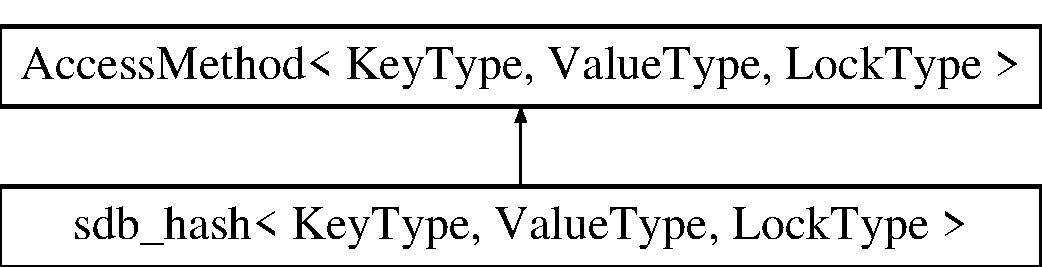
\includegraphics[height=2cm]{classsdb__hash}
\end{center}
\end{figure}
\subsection*{Public Types}
\begin{CompactItemize}
\item 
\hypertarget{classsdb__hash_5968365ee85645ab1b3cdf20a080b96c}{
typedef \hyperlink{classbucket__chain__}{bucket\_\-chain\_\-}$<$ LockType $>$ \textbf{bucket\_\-chain}}
\label{classsdb__hash_5968365ee85645ab1b3cdf20a080b96c}

\item 
\hypertarget{classsdb__hash_99cf7f90f1aabe92eb592ab73cc34eeb}{
typedef std::pair$<$ \hyperlink{classbucket__chain__}{bucket\_\-chain} $\ast$, char $\ast$ $>$ \textbf{SDBCursor}}
\label{classsdb__hash_99cf7f90f1aabe92eb592ab73cc34eeb}

\item 
\hypertarget{classsdb__hash_2af15a87cb82b406d6a79631a2f03431}{
typedef DataType$<$ KeyType, ValueType $>$ \textbf{DataType}}
\label{classsdb__hash_2af15a87cb82b406d6a79631a2f03431}

\end{CompactItemize}
\subsection*{Public Member Functions}
\begin{CompactItemize}
\item 
\hyperlink{classsdb__hash_02cd69cf8f60ae7f8661b1499d49c453}{sdb\_\-hash} (const string \&fileName=\char`\"{}sdb\_\-hash.dat\char`\"{})
\item 
virtual \hyperlink{classsdb__hash_607bf8eee5de43ee297a5e7ef7c0f56d}{$\sim$sdb\_\-hash} ()
\item 
void \hyperlink{classsdb__hash_e56dbe504c8ae570e59a0571f8099b19}{setBucketSize} (size\_\-t bucketSize)
\begin{CompactList}\small\item\em set bucket size of fileHeader \item\end{CompactList}\item 
void \hyperlink{classsdb__hash_50342daffbd37c85755e4f00f11fdf95}{setDegree} (size\_\-t dpow)
\item 
void \hyperlink{classsdb__hash_f6a720d37fabe2b8a8e8bfcd161c2663}{setCacheSize} (size\_\-t cacheSize)
\item 
\hypertarget{classsdb__hash_18d959e4e8bd201f362b8262f6e37716}{
std::string \hyperlink{classsdb__hash_18d959e4e8bd201f362b8262f6e37716}{getFileName} () const }
\label{classsdb__hash_18d959e4e8bd201f362b8262f6e37716}

\begin{CompactList}\small\item\em return the \hyperlink{classfile}{file} name of the SequentialDB \item\end{CompactList}\item 
bool \hyperlink{classsdb__hash_17c82560d424f1d3519e0b4788fd8ef2}{insert} (const DataType \&dat)
\item 
bool \hyperlink{classsdb__hash_4cd4dcd9d599a843b63d7dda5275131f}{insert} (const KeyType \&key, const ValueType \&value)
\item 
ValueType $\ast$ \hyperlink{classsdb__hash_9f39e15dd1c45b2b78b508df26c69568}{find} (const KeyType \&key)
\item 
\hypertarget{classsdb__hash_bd27b5d38ef142e6f2a89733a1213a64}{
bool \textbf{get} (const KeyType \&key, ValueType \&value)}
\label{classsdb__hash_bd27b5d38ef142e6f2a89733a1213a64}

\item 
bool \hyperlink{classsdb__hash_a6ada730f03769b29c7c2e71d97fcd14}{del} (const KeyType \&key)
\item 
bool \hyperlink{classsdb__hash_01a9c2ad383dac61d5e6ff3e20841689}{update} (const DataType \&dat)
\item 
bool \hyperlink{classsdb__hash_d89de45c4ed1d5937fd22745e2a61f20}{update} (const KeyType \&key, const ValueType \&value)
\item 
SDBCursor \hyperlink{classsdb__hash_3594271208cb8aa10beca9f9f16fddd6}{search} (const KeyType \&key)
\item 
bool \hyperlink{classsdb__hash_c229c71b533a2d90941568e6449801db}{search} (const KeyType \&key, SDBCursor \&locn)
\item 
SDBCursor \hyperlink{classsdb__hash_18aa637624e610e99727e368f750cef5}{get\_\-first\_\-locn} ()
\item 
\hypertarget{classsdb__hash_08c49219bfad42f63c2c86f4b180959a}{
bool \textbf{get} (const SDBCursor \&locn, KeyType \&key, ValueType \&value)}
\label{classsdb__hash_08c49219bfad42f63c2c86f4b180959a}

\item 
bool \hyperlink{classsdb__hash_7e501588a5161276baff02c6812aa147}{get} (const SDBCursor \&locn, DataType \&rec)
\item 
bool \hyperlink{classsdb__hash_08fcfc39a846687aa28ecfa4f919f3bc}{seq} (SDBCursor \&locn, DataType \&rec, ESeqDirection sdir=ESD\_\-FORWARD)
\begin{CompactList}\small\item\em sequential access method \item\end{CompactList}\item 
int \hyperlink{classsdb__hash_0abd12e832bafd55d622f67497df47f9}{num\_\-items} ()
\item 
bool \hyperlink{classsdb__hash_323877d8e6fb88a7ac89ff7b361dfa5c}{open} ()
\item 
bool \hyperlink{classsdb__hash_2ebf3f46da2bfa6249badf1d1af352f2}{close} ()
\item 
void \hyperlink{classsdb__hash_23b1c9a395291fbe24416d2e1c24d364}{commit} ()
\item 
void \hyperlink{classsdb__hash_6b9f4c1147c4702b863095a324b81cfb}{flush} ()
\item 
void \hyperlink{classsdb__hash_327527c4f96ea2115450d3b2d0d2ca0d}{display} (std::ostream \&os=std::cout, bool onlyheader=true)
\item 
double \hyperlink{classsdb__hash_23fdd1400cd2c1e7f922b16a8a372924}{loadFactor} ()
\begin{CompactList}\small\item\em It displays how much space has been wasted in percentage after deleting or updates. \item\end{CompactList}\end{CompactItemize}
\subsection*{Protected Types}
\begin{CompactItemize}
\item 
\hypertarget{classsdb__hash_df4db8b80f27271108713daee250bd2f}{
typedef multimap$<$ int, \hyperlink{classbucket__chain__}{bucket\_\-chain} $\ast$, greater$<$ int $>$ $>$::iterator \textbf{CacheIter}}
\label{classsdb__hash_df4db8b80f27271108713daee250bd2f}

\end{CompactItemize}
\subsection*{Protected Attributes}
\begin{CompactItemize}
\item 
\hypertarget{classsdb__hash_176b3804e4064ce796ee50c00c1cef68}{
\hyperlink{classbucket__chain__}{bucket\_\-chain} $\ast$$\ast$ \textbf{entry\_\-}}
\label{classsdb__hash_176b3804e4064ce796ee50c00c1cef68}

\item 
\hypertarget{classsdb__hash_2d79c743b5b5001f7fabefe183d1ee87}{
long $\ast$ \textbf{bucketAddr}}
\label{classsdb__hash_2d79c743b5b5001f7fabefe183d1ee87}

\item 
\hypertarget{classsdb__hash_a9ff81bc12174dab813aa25b1ffb83fc}{
multimap$<$ int, \hyperlink{classbucket__chain__}{bucket\_\-chain} $\ast$, greater$<$ int $>$ $>$ \textbf{sh\_\-cache\_\-}}
\label{classsdb__hash_a9ff81bc12174dab813aa25b1ffb83fc}

\end{CompactItemize}


\subsection{Detailed Description}
\subsubsection*{template$<$typename KeyType, typename ValueType, typename LockType = NullLock$>$ class sdb\_\-hash$<$ KeyType, ValueType, LockType $>$}

\hyperlink{classfile}{file} version of array hash using Cache-Conscious Collision Resolution. 

\hyperlink{classsdb__hash}{sdb\_\-hash} is built on array hash using Cache-Conscious Collision Resolution.

For \hyperlink{classfile}{file} version, there is a little different, each bucket is now a bucket\_\-chain, and each bucket\_\-chain hash fixed size. 

Definition at line 44 of file sdb\_\-hash.h.

\subsection{Constructor \& Destructor Documentation}
\hypertarget{classsdb__hash_02cd69cf8f60ae7f8661b1499d49c453}{
\index{sdb\_\-hash@{sdb\_\-hash}!sdb\_\-hash@{sdb\_\-hash}}
\index{sdb\_\-hash@{sdb\_\-hash}!sdb_hash@{sdb\_\-hash}}
\subsubsection[{sdb\_\-hash}]{\setlength{\rightskip}{0pt plus 5cm}template$<$typename KeyType , typename ValueType , typename LockType  = NullLock$>$ {\bf sdb\_\-hash}$<$ KeyType, ValueType, LockType $>$::{\bf sdb\_\-hash} (const string \& {\em fileName} = {\tt \char`\"{}sdb\_\-hash$<$~KeyType,~ValueType,~LockType~$>$.dat\char`\"{}})\hspace{0.3cm}{\tt  \mbox{[}inline\mbox{]}}}}
\label{classsdb__hash_02cd69cf8f60ae7f8661b1499d49c453}


constructor 

Definition at line 56 of file sdb\_\-hash.h.\hypertarget{classsdb__hash_607bf8eee5de43ee297a5e7ef7c0f56d}{
\index{sdb\_\-hash@{sdb\_\-hash}!$\sim$sdb\_\-hash@{$\sim$sdb\_\-hash}}
\index{$\sim$sdb\_\-hash@{$\sim$sdb\_\-hash}!sdb_hash@{sdb\_\-hash}}
\subsubsection[{$\sim$sdb\_\-hash}]{\setlength{\rightskip}{0pt plus 5cm}template$<$typename KeyType , typename ValueType , typename LockType  = NullLock$>$ virtual {\bf sdb\_\-hash}$<$ KeyType, ValueType, LockType $>$::$\sim${\bf sdb\_\-hash} ()\hspace{0.3cm}{\tt  \mbox{[}inline, virtual\mbox{]}}}}
\label{classsdb__hash_607bf8eee5de43ee297a5e7ef7c0f56d}


deconstructor, \hyperlink{classsdb__hash_2ebf3f46da2bfa6249badf1d1af352f2}{close()} will also be called here. 

Definition at line 66 of file sdb\_\-hash.h.

\subsection{Member Function Documentation}
\hypertarget{classsdb__hash_2ebf3f46da2bfa6249badf1d1af352f2}{
\index{sdb\_\-hash@{sdb\_\-hash}!close@{close}}
\index{close@{close}!sdb_hash@{sdb\_\-hash}}
\subsubsection[{close}]{\setlength{\rightskip}{0pt plus 5cm}template$<$typename KeyType , typename ValueType , typename LockType  = NullLock$>$ bool {\bf sdb\_\-hash}$<$ KeyType, ValueType, LockType $>$::close ()\hspace{0.3cm}{\tt  \mbox{[}inline\mbox{]}}}}
\label{classsdb__hash_2ebf3f46da2bfa6249badf1d1af352f2}


db should be closed after open, and it will automatically called in deconstuctor. 

Definition at line 632 of file sdb\_\-hash.h.\hypertarget{classsdb__hash_23b1c9a395291fbe24416d2e1c24d364}{
\index{sdb\_\-hash@{sdb\_\-hash}!commit@{commit}}
\index{commit@{commit}!sdb_hash@{sdb\_\-hash}}
\subsubsection[{commit}]{\setlength{\rightskip}{0pt plus 5cm}template$<$typename KeyType , typename ValueType , typename LockType  = NullLock$>$ void {\bf sdb\_\-hash}$<$ KeyType, ValueType, LockType $>$::commit ()\hspace{0.3cm}{\tt  \mbox{[}inline\mbox{]}}}}
\label{classsdb__hash_23b1c9a395291fbe24416d2e1c24d364}


write the dirty buckets to disk, not release the memory 

Definition at line 659 of file sdb\_\-hash.h.\hypertarget{classsdb__hash_a6ada730f03769b29c7c2e71d97fcd14}{
\index{sdb\_\-hash@{sdb\_\-hash}!del@{del}}
\index{del@{del}!sdb_hash@{sdb\_\-hash}}
\subsubsection[{del}]{\setlength{\rightskip}{0pt plus 5cm}template$<$typename KeyType , typename ValueType , typename LockType  = NullLock$>$ bool {\bf sdb\_\-hash}$<$ KeyType, ValueType, LockType $>$::del (const KeyType \& {\em key})\hspace{0.3cm}{\tt  \mbox{[}inline\mbox{]}}}}
\label{classsdb__hash_a6ada730f03769b29c7c2e71d97fcd14}


delete an item 

Definition at line 236 of file sdb\_\-hash.h.\hypertarget{classsdb__hash_327527c4f96ea2115450d3b2d0d2ca0d}{
\index{sdb\_\-hash@{sdb\_\-hash}!display@{display}}
\index{display@{display}!sdb_hash@{sdb\_\-hash}}
\subsubsection[{display}]{\setlength{\rightskip}{0pt plus 5cm}template$<$typename KeyType , typename ValueType , typename LockType  = NullLock$>$ void {\bf sdb\_\-hash}$<$ KeyType, ValueType, LockType $>$::display (std::ostream \& {\em os} = {\tt std::cout}, \/  bool {\em onlyheader} = {\tt true})\hspace{0.3cm}{\tt  \mbox{[}inline\mbox{]}}}}
\label{classsdb__hash_327527c4f96ea2115450d3b2d0d2ca0d}


display the info of \hyperlink{classsdb__hash}{sdb\_\-hash} 

Definition at line 702 of file sdb\_\-hash.h.\hypertarget{classsdb__hash_9f39e15dd1c45b2b78b508df26c69568}{
\index{sdb\_\-hash@{sdb\_\-hash}!find@{find}}
\index{find@{find}!sdb_hash@{sdb\_\-hash}}
\subsubsection[{find}]{\setlength{\rightskip}{0pt plus 5cm}template$<$typename KeyType , typename ValueType , typename LockType  = NullLock$>$ ValueType$\ast$ {\bf sdb\_\-hash}$<$ KeyType, ValueType, LockType $>$::find (const KeyType \& {\em key})\hspace{0.3cm}{\tt  \mbox{[}inline\mbox{]}}}}
\label{classsdb__hash_9f39e15dd1c45b2b78b508df26c69568}


find an item, return pointer to the value. Note that, there will be memory leak if not delete the value 

Definition at line 194 of file sdb\_\-hash.h.\hypertarget{classsdb__hash_6b9f4c1147c4702b863095a324b81cfb}{
\index{sdb\_\-hash@{sdb\_\-hash}!flush@{flush}}
\index{flush@{flush}!sdb_hash@{sdb\_\-hash}}
\subsubsection[{flush}]{\setlength{\rightskip}{0pt plus 5cm}template$<$typename KeyType , typename ValueType , typename LockType  = NullLock$>$ void {\bf sdb\_\-hash}$<$ KeyType, ValueType, LockType $>$::flush ()\hspace{0.3cm}{\tt  \mbox{[}inline\mbox{]}}}}
\label{classsdb__hash_6b9f4c1147c4702b863095a324b81cfb}


Write the dirty buckets to disk and also free up most of the memory. Note that, for efficieny, entry\_\-\mbox{[}\mbox{]} is not freed up. 

Definition at line 681 of file sdb\_\-hash.h.\hypertarget{classsdb__hash_7e501588a5161276baff02c6812aa147}{
\index{sdb\_\-hash@{sdb\_\-hash}!get@{get}}
\index{get@{get}!sdb_hash@{sdb\_\-hash}}
\subsubsection[{get}]{\setlength{\rightskip}{0pt plus 5cm}template$<$typename KeyType , typename ValueType , typename LockType  = NullLock$>$ bool {\bf sdb\_\-hash}$<$ KeyType, ValueType, LockType $>$::get (const SDBCursor \& {\em locn}, \/  DataType \& {\em rec})\hspace{0.3cm}{\tt  \mbox{[}inline\mbox{]}}}}
\label{classsdb__hash_7e501588a5161276baff02c6812aa147}


get an item from given SDBCursor 

Definition at line 427 of file sdb\_\-hash.h.\hypertarget{classsdb__hash_18aa637624e610e99727e368f750cef5}{
\index{sdb\_\-hash@{sdb\_\-hash}!get\_\-first\_\-locn@{get\_\-first\_\-locn}}
\index{get\_\-first\_\-locn@{get\_\-first\_\-locn}!sdb_hash@{sdb\_\-hash}}
\subsubsection[{get\_\-first\_\-locn}]{\setlength{\rightskip}{0pt plus 5cm}template$<$typename KeyType , typename ValueType , typename LockType  = NullLock$>$ SDBCursor {\bf sdb\_\-hash}$<$ KeyType, ValueType, LockType $>$::get\_\-first\_\-locn ()\hspace{0.3cm}{\tt  \mbox{[}inline\mbox{]}}}}
\label{classsdb__hash_18aa637624e610e99727e368f750cef5}


get the SDBCursor of first item in the first not empty bucket. 

Definition at line 399 of file sdb\_\-hash.h.\hypertarget{classsdb__hash_4cd4dcd9d599a843b63d7dda5275131f}{
\index{sdb\_\-hash@{sdb\_\-hash}!insert@{insert}}
\index{insert@{insert}!sdb_hash@{sdb\_\-hash}}
\subsubsection[{insert}]{\setlength{\rightskip}{0pt plus 5cm}template$<$typename KeyType , typename ValueType , typename LockType  = NullLock$>$ bool {\bf sdb\_\-hash}$<$ KeyType, ValueType, LockType $>$::insert (const KeyType \& {\em key}, \/  const ValueType \& {\em value})\hspace{0.3cm}{\tt  \mbox{[}inline\mbox{]}}}}
\label{classsdb__hash_4cd4dcd9d599a843b63d7dda5275131f}


insert an item in key/value pair 

Definition at line 125 of file sdb\_\-hash.h.\hypertarget{classsdb__hash_17c82560d424f1d3519e0b4788fd8ef2}{
\index{sdb\_\-hash@{sdb\_\-hash}!insert@{insert}}
\index{insert@{insert}!sdb_hash@{sdb\_\-hash}}
\subsubsection[{insert}]{\setlength{\rightskip}{0pt plus 5cm}template$<$typename KeyType , typename ValueType , typename LockType  = NullLock$>$ bool {\bf sdb\_\-hash}$<$ KeyType, ValueType, LockType $>$::insert (const DataType \& {\em dat})\hspace{0.3cm}{\tt  \mbox{[}inline\mbox{]}}}}
\label{classsdb__hash_17c82560d424f1d3519e0b4788fd8ef2}


insert an item of DataType 

Definition at line 118 of file sdb\_\-hash.h.\hypertarget{classsdb__hash_23fdd1400cd2c1e7f922b16a8a372924}{
\index{sdb\_\-hash@{sdb\_\-hash}!loadFactor@{loadFactor}}
\index{loadFactor@{loadFactor}!sdb_hash@{sdb\_\-hash}}
\subsubsection[{loadFactor}]{\setlength{\rightskip}{0pt plus 5cm}template$<$typename KeyType , typename ValueType , typename LockType  = NullLock$>$ double {\bf sdb\_\-hash}$<$ KeyType, ValueType, LockType $>$::loadFactor ()\hspace{0.3cm}{\tt  \mbox{[}inline\mbox{]}}}}
\label{classsdb__hash_23fdd1400cd2c1e7f922b16a8a372924}


It displays how much space has been wasted in percentage after deleting or updates. 

when an item is deleted, we don't release its space in disk but set a flag that it have been deleted. And it will lead to low efficiency. Maybe we should dump it to another files when loadFactor are low. 

Definition at line 728 of file sdb\_\-hash.h.\hypertarget{classsdb__hash_0abd12e832bafd55d622f67497df47f9}{
\index{sdb\_\-hash@{sdb\_\-hash}!num\_\-items@{num\_\-items}}
\index{num\_\-items@{num\_\-items}!sdb_hash@{sdb\_\-hash}}
\subsubsection[{num\_\-items}]{\setlength{\rightskip}{0pt plus 5cm}template$<$typename KeyType , typename ValueType , typename LockType  = NullLock$>$ int {\bf sdb\_\-hash}$<$ KeyType, ValueType, LockType $>$::num\_\-items ()\hspace{0.3cm}{\tt  \mbox{[}inline\mbox{]}}}}
\label{classsdb__hash_0abd12e832bafd55d622f67497df47f9}


get the num of items 

Definition at line 559 of file sdb\_\-hash.h.\hypertarget{classsdb__hash_323877d8e6fb88a7ac89ff7b361dfa5c}{
\index{sdb\_\-hash@{sdb\_\-hash}!open@{open}}
\index{open@{open}!sdb_hash@{sdb\_\-hash}}
\subsubsection[{open}]{\setlength{\rightskip}{0pt plus 5cm}template$<$typename KeyType , typename ValueType , typename LockType  = NullLock$>$ bool {\bf sdb\_\-hash}$<$ KeyType, ValueType, LockType $>$::open ()\hspace{0.3cm}{\tt  \mbox{[}inline\mbox{]}}}}
\label{classsdb__hash_323877d8e6fb88a7ac89ff7b361dfa5c}


db must be opened to be used. 

Definition at line 567 of file sdb\_\-hash.h.\hypertarget{classsdb__hash_c229c71b533a2d90941568e6449801db}{
\index{sdb\_\-hash@{sdb\_\-hash}!search@{search}}
\index{search@{search}!sdb_hash@{sdb\_\-hash}}
\subsubsection[{search}]{\setlength{\rightskip}{0pt plus 5cm}template$<$typename KeyType , typename ValueType , typename LockType  = NullLock$>$ bool {\bf sdb\_\-hash}$<$ KeyType, ValueType, LockType $>$::search (const KeyType \& {\em key}, \/  SDBCursor \& {\em locn})\hspace{0.3cm}{\tt  \mbox{[}inline\mbox{]}}}}
\label{classsdb__hash_c229c71b533a2d90941568e6449801db}


another search function, flushCache\_\-() will be called at the beginning, 

Definition at line 331 of file sdb\_\-hash.h.\hypertarget{classsdb__hash_3594271208cb8aa10beca9f9f16fddd6}{
\index{sdb\_\-hash@{sdb\_\-hash}!search@{search}}
\index{search@{search}!sdb_hash@{sdb\_\-hash}}
\subsubsection[{search}]{\setlength{\rightskip}{0pt plus 5cm}template$<$typename KeyType , typename ValueType , typename LockType  = NullLock$>$ SDBCursor {\bf sdb\_\-hash}$<$ KeyType, ValueType, LockType $>$::search (const KeyType \& {\em key})\hspace{0.3cm}{\tt  \mbox{[}inline\mbox{]}}}}
\label{classsdb__hash_3594271208cb8aa10beca9f9f16fddd6}


search an item

\begin{Desc}
\item[Returns:]SDBCursor \end{Desc}


Definition at line 320 of file sdb\_\-hash.h.\hypertarget{classsdb__hash_08fcfc39a846687aa28ecfa4f919f3bc}{
\index{sdb\_\-hash@{sdb\_\-hash}!seq@{seq}}
\index{seq@{seq}!sdb_hash@{sdb\_\-hash}}
\subsubsection[{seq}]{\setlength{\rightskip}{0pt plus 5cm}template$<$typename KeyType , typename ValueType , typename LockType  = NullLock$>$ bool {\bf sdb\_\-hash}$<$ KeyType, ValueType, LockType $>$::seq (SDBCursor \& {\em locn}, \/  DataType \& {\em rec}, \/  ESeqDirection {\em sdir} = {\tt ESD\_\-FORWARD})\hspace{0.3cm}{\tt  \mbox{[}inline\mbox{]}}}}
\label{classsdb__hash_08fcfc39a846687aa28ecfa4f919f3bc}


sequential access method 

\begin{Desc}
\item[Parameters:]
\begin{description}
\item[{\em locn}]is the current SDBCursor, and will replaced next SDBCursor when route finished. \item[{\em rec}]is the item in SDBCursor locn. \item[{\em sdir}]is sequential access direction, for hash is unordered, we only implement forward case. \end{description}
\end{Desc}


Definition at line 470 of file sdb\_\-hash.h.\hypertarget{classsdb__hash_e56dbe504c8ae570e59a0571f8099b19}{
\index{sdb\_\-hash@{sdb\_\-hash}!setBucketSize@{setBucketSize}}
\index{setBucketSize@{setBucketSize}!sdb_hash@{sdb\_\-hash}}
\subsubsection[{setBucketSize}]{\setlength{\rightskip}{0pt plus 5cm}template$<$typename KeyType , typename ValueType , typename LockType  = NullLock$>$ void {\bf sdb\_\-hash}$<$ KeyType, ValueType, LockType $>$::setBucketSize (size\_\-t {\em bucketSize})\hspace{0.3cm}{\tt  \mbox{[}inline\mbox{]}}}}
\label{classsdb__hash_e56dbe504c8ae570e59a0571f8099b19}


set bucket size of fileHeader 

if not called use default size 8192 

Definition at line 75 of file sdb\_\-hash.h.\hypertarget{classsdb__hash_f6a720d37fabe2b8a8e8bfcd161c2663}{
\index{sdb\_\-hash@{sdb\_\-hash}!setCacheSize@{setCacheSize}}
\index{setCacheSize@{setCacheSize}!sdb_hash@{sdb\_\-hash}}
\subsubsection[{setCacheSize}]{\setlength{\rightskip}{0pt plus 5cm}template$<$typename KeyType , typename ValueType , typename LockType  = NullLock$>$ void {\bf sdb\_\-hash}$<$ KeyType, ValueType, LockType $>$::setCacheSize (size\_\-t {\em cacheSize})\hspace{0.3cm}{\tt  \mbox{[}inline\mbox{]}}}}
\label{classsdb__hash_f6a720d37fabe2b8a8e8bfcd161c2663}


set cache size, if not called use default size 100000 

Definition at line 101 of file sdb\_\-hash.h.\hypertarget{classsdb__hash_50342daffbd37c85755e4f00f11fdf95}{
\index{sdb\_\-hash@{sdb\_\-hash}!setDegree@{setDegree}}
\index{setDegree@{setDegree}!sdb_hash@{sdb\_\-hash}}
\subsubsection[{setDegree}]{\setlength{\rightskip}{0pt plus 5cm}template$<$typename KeyType , typename ValueType , typename LockType  = NullLock$>$ void {\bf sdb\_\-hash}$<$ KeyType, ValueType, LockType $>$::setDegree (size\_\-t {\em dpow})\hspace{0.3cm}{\tt  \mbox{[}inline\mbox{]}}}}
\label{classsdb__hash_50342daffbd37c85755e4f00f11fdf95}


set directory size if fileHeader

if not called use default size 4096 

Definition at line 90 of file sdb\_\-hash.h.\hypertarget{classsdb__hash_d89de45c4ed1d5937fd22745e2a61f20}{
\index{sdb\_\-hash@{sdb\_\-hash}!update@{update}}
\index{update@{update}!sdb_hash@{sdb\_\-hash}}
\subsubsection[{update}]{\setlength{\rightskip}{0pt plus 5cm}template$<$typename KeyType , typename ValueType , typename LockType  = NullLock$>$ bool {\bf sdb\_\-hash}$<$ KeyType, ValueType, LockType $>$::update (const KeyType \& {\em key}, \/  const ValueType \& {\em value})\hspace{0.3cm}{\tt  \mbox{[}inline\mbox{]}}}}
\label{classsdb__hash_d89de45c4ed1d5937fd22745e2a61f20}


update an item by key/value pair 

Definition at line 275 of file sdb\_\-hash.h.\hypertarget{classsdb__hash_01a9c2ad383dac61d5e6ff3e20841689}{
\index{sdb\_\-hash@{sdb\_\-hash}!update@{update}}
\index{update@{update}!sdb_hash@{sdb\_\-hash}}
\subsubsection[{update}]{\setlength{\rightskip}{0pt plus 5cm}template$<$typename KeyType , typename ValueType , typename LockType  = NullLock$>$ bool {\bf sdb\_\-hash}$<$ KeyType, ValueType, LockType $>$::update (const DataType \& {\em dat})\hspace{0.3cm}{\tt  \mbox{[}inline\mbox{]}}}}
\label{classsdb__hash_01a9c2ad383dac61d5e6ff3e20841689}


update an item through DataType data 

Definition at line 267 of file sdb\_\-hash.h.

The documentation for this class was generated from the following file:\begin{CompactItemize}
\item 
/home/Kevin/izenelib/include/am/sdb\_\-hash/\hyperlink{sdb__hash_8h}{sdb\_\-hash.h}\end{CompactItemize}

\hypertarget{classsdb__hashing}{
\section{sdb\_\-hashing Class Reference}
\label{classsdb__hashing}\index{sdb\_\-hashing@{sdb\_\-hashing}}
}
hashing function object used for \hyperlink{classsdb__hash}{sdb\_\-hash}  


{\tt \#include $<$sdb\_\-hash\_\-types.h$>$}

\subsection*{Static Public Member Functions}
\begin{CompactItemize}
\item 
\hypertarget{classsdb__hashing_555fa4737785d01b8c535378cc9e092b}{
static uint32\_\-t \textbf{hash\_\-fun} (const void $\ast$kbuf, const size\_\-t ksize)}
\label{classsdb__hashing_555fa4737785d01b8c535378cc9e092b}

\end{CompactItemize}


\subsection{Detailed Description}
hashing function object used for \hyperlink{classsdb__hash}{sdb\_\-hash} 

Definition at line 34 of file sdb\_\-hash\_\-types.h.

The documentation for this class was generated from the following file:\begin{CompactItemize}
\item 
/home/Kevin/izenelib/include/am/sdb\_\-hash/sdb\_\-hash\_\-types.h\end{CompactItemize}

\hypertarget{structShFileHeader}{
\section{ShFileHeader Struct Reference}
\label{structShFileHeader}\index{ShFileHeader@{ShFileHeader}}
}
FileHeader of \hyperlink{classsdb__hash}{sdb\_\-hash}.  


{\tt \#include $<$sdb\_\-hash\_\-header.h$>$}

\subsection*{Public Member Functions}
\begin{CompactItemize}
\item 
\hypertarget{structShFileHeader_e72562555d56702b9b843cd453d33227}{
void \textbf{display} (std::ostream \&os=std::cout)}
\label{structShFileHeader_e72562555d56702b9b843cd453d33227}

\item 
\hypertarget{structShFileHeader_42d12da07006c4bc76126aed2c7d0acb}{
bool \textbf{toFile} (FILE $\ast$f)}
\label{structShFileHeader_42d12da07006c4bc76126aed2c7d0acb}

\item 
\hypertarget{structShFileHeader_68d65a0a55f43a9fa163a996b06bc3cf}{
bool \textbf{fromFile} (FILE $\ast$f)}
\label{structShFileHeader_68d65a0a55f43a9fa163a996b06bc3cf}

\end{CompactItemize}
\subsection*{Public Attributes}
\begin{CompactItemize}
\item 
\hypertarget{structShFileHeader_1ad9263cd23d28671094a6a9a1f1d734}{
int \textbf{magic}}
\label{structShFileHeader_1ad9263cd23d28671094a6a9a1f1d734}

\item 
\hypertarget{structShFileHeader_c11dce06e778659fa764ff21003453a0}{
size\_\-t \textbf{bucketSize}}
\label{structShFileHeader_c11dce06e778659fa764ff21003453a0}

\item 
\hypertarget{structShFileHeader_bcfafc98d47e19620789cbc93a085f68}{
size\_\-t \textbf{dpow}}
\label{structShFileHeader_bcfafc98d47e19620789cbc93a085f68}

\item 
\hypertarget{structShFileHeader_d38f080419e34336c4b41b6c41c3bef3}{
size\_\-t \textbf{cacheSize}}
\label{structShFileHeader_d38f080419e34336c4b41b6c41c3bef3}

\item 
\hypertarget{structShFileHeader_f5a9cf6ff176e492fac5764fcc0523b1}{
size\_\-t \textbf{numItems}}
\label{structShFileHeader_f5a9cf6ff176e492fac5764fcc0523b1}

\item 
\hypertarget{structShFileHeader_48260cd93890486f6d1a2c3d750b5897}{
size\_\-t \textbf{nBlock}}
\label{structShFileHeader_48260cd93890486f6d1a2c3d750b5897}

\end{CompactItemize}


\subsection{Detailed Description}
FileHeader of \hyperlink{classsdb__hash}{sdb\_\-hash}. 

Definition at line 14 of file sdb\_\-hash\_\-header.h.

The documentation for this struct was generated from the following file:\begin{CompactItemize}
\item 
/home/Kevin/izenelib/include/am/sdb\_\-hash/sdb\_\-hash\_\-header.h\end{CompactItemize}

\hypertarget{classSkipList_3_01ValueType_00_01KeyType_00_01MAX__GAP_00_01MemStorage_00_01LockType_01_4}{
\section{SkipList$<$ ValueType, KeyType, MAX\_\-GAP, MemStorage, LockType $>$ Class Template Reference}
\label{classSkipList_3_01ValueType_00_01KeyType_00_01MAX__GAP_00_01MemStorage_00_01LockType_01_4}\index{SkipList$<$ ValueType, KeyType, MAX\_\-GAP, MemStorage, LockType $>$@{SkipList$<$ ValueType, KeyType, MAX\_\-GAP, MemStorage, LockType $>$}}
}
The definition and implementation of the SkipList(Actually, it is a deterministic skip list).  


{\tt \#include $<$skip\_\-list.hpp$>$}

Inheritance diagram for SkipList$<$ ValueType, KeyType, MAX\_\-GAP, MemStorage, LockType $>$::\begin{figure}[H]
\begin{center}
\leavevmode
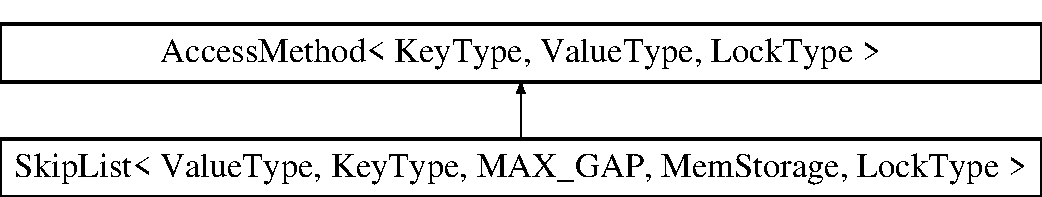
\includegraphics[height=2cm]{classSkipList_3_01ValueType_00_01KeyType_00_01MAX__GAP_00_01MemStorage_00_01LockType_01_4}
\end{center}
\end{figure}
\subsection*{Classes}
\begin{CompactItemize}
\item 
class \textbf{SkipNode}
\begin{CompactList}\small\item\em \hyperlink{classSkipNode}{SkipNode} reprents a node in a SkipList. \item\end{CompactList}\end{CompactItemize}
\subsection*{Public Member Functions}
\begin{CompactItemize}
\item 
\hyperlink{classSkipList_3_01ValueType_00_01KeyType_00_01MAX__GAP_00_01MemStorage_00_01LockType_01_4_625716dcaac1e6d5250135d0ed008f48}{SkipList} ()
\begin{CompactList}\small\item\em Construct the tree. \item\end{CompactList}\item 
\hyperlink{classSkipList_3_01ValueType_00_01KeyType_00_01MAX__GAP_00_01MemStorage_00_01LockType_01_4_c7c90a05082f010951c52e7c5b508b24}{SkipList} (const \hyperlink{classSkipList_3_01ValueType_00_01KeyType_00_01MAX__GAP_00_01MemStorage_00_01LockType_01_4}{Self} \&rhs)
\begin{CompactList}\small\item\em Copy constructor. \item\end{CompactList}\item 
\hypertarget{classSkipList_3_01ValueType_00_01KeyType_00_01MAX__GAP_00_01MemStorage_00_01LockType_01_4_4a79a8e09210a216dbe459c0b57e301a}{
\hyperlink{classSkipList_3_01ValueType_00_01KeyType_00_01MAX__GAP_00_01MemStorage_00_01LockType_01_4_4a79a8e09210a216dbe459c0b57e301a}{$\sim$SkipList} ()}
\label{classSkipList_3_01ValueType_00_01KeyType_00_01MAX__GAP_00_01MemStorage_00_01LockType_01_4_4a79a8e09210a216dbe459c0b57e301a}

\begin{CompactList}\small\item\em Destructor. \item\end{CompactList}\item 
const ValueType $\ast$ \hyperlink{classSkipList_3_01ValueType_00_01KeyType_00_01MAX__GAP_00_01MemStorage_00_01LockType_01_4_3a779082b51cc31b13d0cd88931f6952}{find\_\-min} () const 
\begin{CompactList}\small\item\em Find the smallest item in the tree. \item\end{CompactList}\item 
const ValueType $\ast$ \hyperlink{classSkipList_3_01ValueType_00_01KeyType_00_01MAX__GAP_00_01MemStorage_00_01LockType_01_4_b9bd70f284edf7639c7f2320fe39176a}{find\_\-max} () const 
\begin{CompactList}\small\item\em Find the largest item in the tree. \item\end{CompactList}\item 
virtual ValueType $\ast$ \hyperlink{classSkipList_3_01ValueType_00_01KeyType_00_01MAX__GAP_00_01MemStorage_00_01LockType_01_4_fb164870329e594f7e8ab87df47ff502}{find} (const KeyType \&v)
\begin{CompactList}\small\item\em Find item x in the tree. \item\end{CompactList}\item 
\hypertarget{classSkipList_3_01ValueType_00_01KeyType_00_01MAX__GAP_00_01MemStorage_00_01LockType_01_4_72102b0600d0ba4c9405aae736aa48bd}{
const ValueType $\ast$ \textbf{find} (const KeyType \&x) const }
\label{classSkipList_3_01ValueType_00_01KeyType_00_01MAX__GAP_00_01MemStorage_00_01LockType_01_4_72102b0600d0ba4c9405aae736aa48bd}

\item 
bool \hyperlink{classSkipList_3_01ValueType_00_01KeyType_00_01MAX__GAP_00_01MemStorage_00_01LockType_01_4_fa6a9e000dee4c64e85d3e4ada7efae1}{is\_\-empty} () const 
\begin{CompactList}\small\item\em Test if the tree is logically empty. \item\end{CompactList}\item 
\hypertarget{classSkipList_3_01ValueType_00_01KeyType_00_01MAX__GAP_00_01MemStorage_00_01LockType_01_4_7e5769303e900cd31a0c41321fd85322}{
void \hyperlink{classSkipList_3_01ValueType_00_01KeyType_00_01MAX__GAP_00_01MemStorage_00_01LockType_01_4_7e5769303e900cd31a0c41321fd85322}{display} (std::ostream \&stream) const }
\label{classSkipList_3_01ValueType_00_01KeyType_00_01MAX__GAP_00_01MemStorage_00_01LockType_01_4_7e5769303e900cd31a0c41321fd85322}

\begin{CompactList}\small\item\em Print the SkipList. \item\end{CompactList}\item 
\hypertarget{classSkipList_3_01ValueType_00_01KeyType_00_01MAX__GAP_00_01MemStorage_00_01LockType_01_4_2578ac7158c6634ab984f6c5cb8e67e7}{
int \textbf{getSize} () const }
\label{classSkipList_3_01ValueType_00_01KeyType_00_01MAX__GAP_00_01MemStorage_00_01LockType_01_4_2578ac7158c6634ab984f6c5cb8e67e7}

\item 
\hypertarget{classSkipList_3_01ValueType_00_01KeyType_00_01MAX__GAP_00_01MemStorage_00_01LockType_01_4_537eaa21e761eb40aa29d487b01c31bd}{
void \hyperlink{classSkipList_3_01ValueType_00_01KeyType_00_01MAX__GAP_00_01MemStorage_00_01LockType_01_4_537eaa21e761eb40aa29d487b01c31bd}{release} ()}
\label{classSkipList_3_01ValueType_00_01KeyType_00_01MAX__GAP_00_01MemStorage_00_01LockType_01_4_537eaa21e761eb40aa29d487b01c31bd}

\begin{CompactList}\small\item\em Make the tree logically empty. \item\end{CompactList}\item 
\hypertarget{classSkipList_3_01ValueType_00_01KeyType_00_01MAX__GAP_00_01MemStorage_00_01LockType_01_4_cc0a8c1df0eed6063ae5ca43e090bb53}{
virtual bool \textbf{insert} (const DataType$<$ KeyType, ValueType $>$ \&data)}
\label{classSkipList_3_01ValueType_00_01KeyType_00_01MAX__GAP_00_01MemStorage_00_01LockType_01_4_cc0a8c1df0eed6063ae5ca43e090bb53}

\item 
\hypertarget{classSkipList_3_01ValueType_00_01KeyType_00_01MAX__GAP_00_01MemStorage_00_01LockType_01_4_cf53180a75a050d2a4e47eebd584dfc3}{
virtual bool \hyperlink{classSkipList_3_01ValueType_00_01KeyType_00_01MAX__GAP_00_01MemStorage_00_01LockType_01_4_cf53180a75a050d2a4e47eebd584dfc3}{insert} (const KeyType \&key, const ValueType \&data)}
\label{classSkipList_3_01ValueType_00_01KeyType_00_01MAX__GAP_00_01MemStorage_00_01LockType_01_4_cf53180a75a050d2a4e47eebd584dfc3}

\begin{CompactList}\small\item\em Insert item x into the SkipList. \item\end{CompactList}\item 
\hypertarget{classSkipList_3_01ValueType_00_01KeyType_00_01MAX__GAP_00_01MemStorage_00_01LockType_01_4_658578f6e15d56c053558e6f793a35c1}{
virtual bool \textbf{del} (const KeyType \&v)}
\label{classSkipList_3_01ValueType_00_01KeyType_00_01MAX__GAP_00_01MemStorage_00_01LockType_01_4_658578f6e15d56c053558e6f793a35c1}

\item 
\hypertarget{classSkipList_3_01ValueType_00_01KeyType_00_01MAX__GAP_00_01MemStorage_00_01LockType_01_4_cebdb64a34d39bc7391cc7b68674bb43}{
virtual bool \textbf{update} (const DataType$<$ KeyType, ValueType $>$ \&data)}
\label{classSkipList_3_01ValueType_00_01KeyType_00_01MAX__GAP_00_01MemStorage_00_01LockType_01_4_cebdb64a34d39bc7391cc7b68674bb43}

\item 
\hypertarget{classSkipList_3_01ValueType_00_01KeyType_00_01MAX__GAP_00_01MemStorage_00_01LockType_01_4_47126dcf071ccd92ac095d8c2bf4e840}{
virtual bool \textbf{update} (const KeyType \&key, const ValueType \&data)}
\label{classSkipList_3_01ValueType_00_01KeyType_00_01MAX__GAP_00_01MemStorage_00_01LockType_01_4_47126dcf071ccd92ac095d8c2bf4e840}

\end{CompactItemize}


\subsection{Detailed Description}
\subsubsection*{template$<$class ValueType, class KeyType, int MAX\_\-GAP, class LockType$>$ class SkipList$<$ ValueType, KeyType, MAX\_\-GAP, MemStorage, LockType $>$}

The definition and implementation of the SkipList(Actually, it is a deterministic skip list). 

Definition at line 124 of file skip\_\-list.hpp.

\subsection{Constructor \& Destructor Documentation}
\hypertarget{classSkipList_3_01ValueType_00_01KeyType_00_01MAX__GAP_00_01MemStorage_00_01LockType_01_4_625716dcaac1e6d5250135d0ed008f48}{
\index{SkipList$<$ ValueType, KeyType, MAX\_\-GAP, MemStorage, LockType $>$@{SkipList$<$ ValueType, KeyType, MAX\_\-GAP, MemStorage, LockType $>$}!SkipList@{SkipList}}
\index{SkipList@{SkipList}!SkipList< ValueType, KeyType, MAX_GAP, MemStorage, LockType >@{SkipList$<$ ValueType, KeyType, MAX\_\-GAP, MemStorage, LockType $>$}}
\subsubsection[{SkipList}]{\setlength{\rightskip}{0pt plus 5cm}template$<$class ValueType , class KeyType , int MAX\_\-GAP, class LockType $>$ SkipList$<$ ValueType, KeyType, MAX\_\-GAP, MemStorage, LockType $>$::SkipList ()\hspace{0.3cm}{\tt  \mbox{[}inline, explicit\mbox{]}}}}
\label{classSkipList_3_01ValueType_00_01KeyType_00_01MAX__GAP_00_01MemStorage_00_01LockType_01_4_625716dcaac1e6d5250135d0ed008f48}


Construct the tree. 

inf is the largest DataType and is used to signal failed finds. 

Definition at line 183 of file skip\_\-list.hpp.\hypertarget{classSkipList_3_01ValueType_00_01KeyType_00_01MAX__GAP_00_01MemStorage_00_01LockType_01_4_c7c90a05082f010951c52e7c5b508b24}{
\index{SkipList$<$ ValueType, KeyType, MAX\_\-GAP, MemStorage, LockType $>$@{SkipList$<$ ValueType, KeyType, MAX\_\-GAP, MemStorage, LockType $>$}!SkipList@{SkipList}}
\index{SkipList@{SkipList}!SkipList< ValueType, KeyType, MAX_GAP, MemStorage, LockType >@{SkipList$<$ ValueType, KeyType, MAX\_\-GAP, MemStorage, LockType $>$}}
\subsubsection[{SkipList}]{\setlength{\rightskip}{0pt plus 5cm}template$<$class ValueType , class KeyType , int MAX\_\-GAP, class LockType $>$ SkipList$<$ ValueType, KeyType, MAX\_\-GAP, MemStorage, LockType $>$::SkipList (const {\bf Self} \& {\em rhs})\hspace{0.3cm}{\tt  \mbox{[}inline\mbox{]}}}}
\label{classSkipList_3_01ValueType_00_01KeyType_00_01MAX__GAP_00_01MemStorage_00_01LockType_01_4_c7c90a05082f010951c52e7c5b508b24}


Copy constructor. 

Not implemented yet. 

Definition at line 206 of file skip\_\-list.hpp.

\subsection{Member Function Documentation}
\hypertarget{classSkipList_3_01ValueType_00_01KeyType_00_01MAX__GAP_00_01MemStorage_00_01LockType_01_4_fb164870329e594f7e8ab87df47ff502}{
\index{SkipList$<$ ValueType, KeyType, MAX\_\-GAP, MemStorage, LockType $>$@{SkipList$<$ ValueType, KeyType, MAX\_\-GAP, MemStorage, LockType $>$}!find@{find}}
\index{find@{find}!SkipList< ValueType, KeyType, MAX_GAP, MemStorage, LockType >@{SkipList$<$ ValueType, KeyType, MAX\_\-GAP, MemStorage, LockType $>$}}
\subsubsection[{find}]{\setlength{\rightskip}{0pt plus 5cm}template$<$class ValueType , class KeyType , int MAX\_\-GAP, class LockType $>$ virtual ValueType$\ast$ SkipList$<$ ValueType, KeyType, MAX\_\-GAP, MemStorage, LockType $>$::find (const KeyType \& {\em v})\hspace{0.3cm}{\tt  \mbox{[}inline, virtual\mbox{]}}}}
\label{classSkipList_3_01ValueType_00_01KeyType_00_01MAX__GAP_00_01MemStorage_00_01LockType_01_4_fb164870329e594f7e8ab87df47ff502}


Find item x in the tree. 

Return the matching item or m\_\-infinity if not found. 

Definition at line 272 of file skip\_\-list.hpp.\hypertarget{classSkipList_3_01ValueType_00_01KeyType_00_01MAX__GAP_00_01MemStorage_00_01LockType_01_4_b9bd70f284edf7639c7f2320fe39176a}{
\index{SkipList$<$ ValueType, KeyType, MAX\_\-GAP, MemStorage, LockType $>$@{SkipList$<$ ValueType, KeyType, MAX\_\-GAP, MemStorage, LockType $>$}!find\_\-max@{find\_\-max}}
\index{find\_\-max@{find\_\-max}!SkipList< ValueType, KeyType, MAX_GAP, MemStorage, LockType >@{SkipList$<$ ValueType, KeyType, MAX\_\-GAP, MemStorage, LockType $>$}}
\subsubsection[{find\_\-max}]{\setlength{\rightskip}{0pt plus 5cm}template$<$class ValueType , class KeyType , int MAX\_\-GAP, class LockType $>$ const ValueType$\ast$ SkipList$<$ ValueType, KeyType, MAX\_\-GAP, MemStorage, LockType $>$::find\_\-max () const\hspace{0.3cm}{\tt  \mbox{[}inline\mbox{]}}}}
\label{classSkipList_3_01ValueType_00_01KeyType_00_01MAX__GAP_00_01MemStorage_00_01LockType_01_4_b9bd70f284edf7639c7f2320fe39176a}


Find the largest item in the tree. 

Return the largest item or m\_\-infinity if empty. 

Definition at line 246 of file skip\_\-list.hpp.\hypertarget{classSkipList_3_01ValueType_00_01KeyType_00_01MAX__GAP_00_01MemStorage_00_01LockType_01_4_3a779082b51cc31b13d0cd88931f6952}{
\index{SkipList$<$ ValueType, KeyType, MAX\_\-GAP, MemStorage, LockType $>$@{SkipList$<$ ValueType, KeyType, MAX\_\-GAP, MemStorage, LockType $>$}!find\_\-min@{find\_\-min}}
\index{find\_\-min@{find\_\-min}!SkipList< ValueType, KeyType, MAX_GAP, MemStorage, LockType >@{SkipList$<$ ValueType, KeyType, MAX\_\-GAP, MemStorage, LockType $>$}}
\subsubsection[{find\_\-min}]{\setlength{\rightskip}{0pt plus 5cm}template$<$class ValueType , class KeyType , int MAX\_\-GAP, class LockType $>$ const ValueType$\ast$ SkipList$<$ ValueType, KeyType, MAX\_\-GAP, MemStorage, LockType $>$::find\_\-min () const\hspace{0.3cm}{\tt  \mbox{[}inline\mbox{]}}}}
\label{classSkipList_3_01ValueType_00_01KeyType_00_01MAX__GAP_00_01MemStorage_00_01LockType_01_4_3a779082b51cc31b13d0cd88931f6952}


Find the smallest item in the tree. 

Return smallest item or m\_\-infinity if empty. 

Definition at line 229 of file skip\_\-list.hpp.\hypertarget{classSkipList_3_01ValueType_00_01KeyType_00_01MAX__GAP_00_01MemStorage_00_01LockType_01_4_fa6a9e000dee4c64e85d3e4ada7efae1}{
\index{SkipList$<$ ValueType, KeyType, MAX\_\-GAP, MemStorage, LockType $>$@{SkipList$<$ ValueType, KeyType, MAX\_\-GAP, MemStorage, LockType $>$}!is\_\-empty@{is\_\-empty}}
\index{is\_\-empty@{is\_\-empty}!SkipList< ValueType, KeyType, MAX_GAP, MemStorage, LockType >@{SkipList$<$ ValueType, KeyType, MAX\_\-GAP, MemStorage, LockType $>$}}
\subsubsection[{is\_\-empty}]{\setlength{\rightskip}{0pt plus 5cm}template$<$class ValueType , class KeyType , int MAX\_\-GAP, class LockType $>$ bool SkipList$<$ ValueType, KeyType, MAX\_\-GAP, MemStorage, LockType $>$::is\_\-empty () const\hspace{0.3cm}{\tt  \mbox{[}inline\mbox{]}}}}
\label{classSkipList_3_01ValueType_00_01KeyType_00_01MAX__GAP_00_01MemStorage_00_01LockType_01_4_fa6a9e000dee4c64e85d3e4ada7efae1}


Test if the tree is logically empty. 

Return true if empty, false otherwise. 

Definition at line 299 of file skip\_\-list.hpp.

The documentation for this class was generated from the following file:\begin{CompactItemize}
\item 
/home/Kevin/izenelib/include/am/skip\_\-list/skip\_\-list.hpp\end{CompactItemize}

\hypertarget{classSkipListFile}{
\section{SkipListFile$<$ KeyType, ValueType, LockType, Alloc $>$ Class Template Reference}
\label{classSkipListFile}\index{SkipListFile@{SkipListFile}}
}
The definition and implementation of the SkipList.  


{\tt \#include $<$SkipListFile.h$>$}

Inheritance diagram for SkipListFile$<$ KeyType, ValueType, LockType, Alloc $>$::\begin{figure}[H]
\begin{center}
\leavevmode
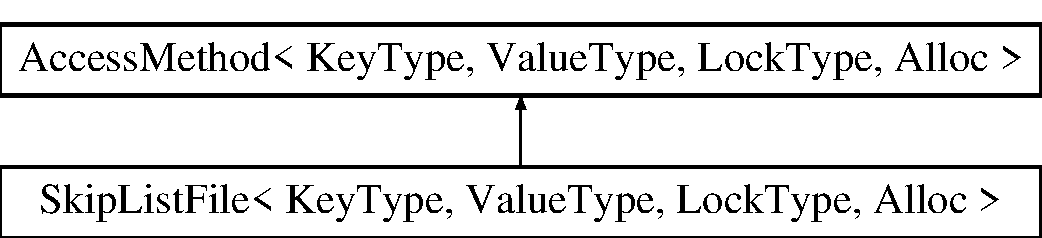
\includegraphics[height=2cm]{classSkipListFile}
\end{center}
\end{figure}
\subsection*{Public Types}
\begin{CompactItemize}
\item 
\hypertarget{classSkipListFile_bd531a90961483899addb340a9486c57}{
typedef DataType$<$ KeyType, ValueType $>$ \textbf{DataType}}
\label{classSkipListFile_bd531a90961483899addb340a9486c57}

\item 
\hypertarget{classSkipListFile_13f97d1caf0f235e7df3b946d60b42cf}{
typedef \hyperlink{classSkipNode}{SkipNode}$<$ DataType, LockType, Alloc $>$ \textbf{SkipNode}}
\label{classSkipListFile_13f97d1caf0f235e7df3b946d60b42cf}

\item 
\hypertarget{classSkipListFile_a6dafe425889dee183978a3e512e8fec}{
typedef \hyperlink{classSkipNode}{SkipNode} $\ast$ \textbf{SDBCursor}}
\label{classSkipListFile_a6dafe425889dee183978a3e512e8fec}

\end{CompactItemize}
\subsection*{Public Member Functions}
\begin{CompactItemize}
\item 
\hyperlink{classSkipListFile_7be7790d5ea16f3261db01afb62b55e1}{SkipListFile} (const std::string \&fileName)
\item 
virtual \hyperlink{classSkipListFile_d233c08a7814bff2e1e535de1414f799}{$\sim$SkipListFile} ()
\begin{CompactList}\small\item\em Destructor. \item\end{CompactList}\item 
void \hyperlink{classSkipListFile_b8a6cbf9fb0386dd4eb965b2aad18f53}{setPageSize} (size\_\-t maxDataSize)
\item 
\hypertarget{classSkipListFile_940d6fda21e881c4fed93dc91a44ba97}{
void \textbf{setDegree} (int degree)}
\label{classSkipListFile_940d6fda21e881c4fed93dc91a44ba97}

\item 
\hypertarget{classSkipListFile_4cb6941e68b83ee403da711596320f19}{
std::string \hyperlink{classSkipListFile_4cb6941e68b83ee403da711596320f19}{getFileName} () const }
\label{classSkipListFile_4cb6941e68b83ee403da711596320f19}

\begin{CompactList}\small\item\em return the \hyperlink{classfile}{file} name of the SequentialDB \item\end{CompactList}\item 
void \hyperlink{classSkipListFile_33f3d7ea02a004d7fdedffe582f2ea72}{setCacheSize} (size\_\-t sz)
\item 
ValueType $\ast$ \hyperlink{classSkipListFile_d5991f6c784169c5cf582d9700eb7d78}{find} (const KeyType \&x)
\begin{CompactList}\small\item\em Find item x in the tree. \item\end{CompactList}\item 
\hypertarget{classSkipListFile_02c3a0a04f7dfa5951d79bf31c6a68a1}{
bool \hyperlink{classSkipListFile_02c3a0a04f7dfa5951d79bf31c6a68a1}{update} (const KeyType \&key, const ValueType \&val)}
\label{classSkipListFile_02c3a0a04f7dfa5951d79bf31c6a68a1}

\begin{CompactList}\small\item\em updata an item with given key, if it not exist, insert it directly. \item\end{CompactList}\item 
\hypertarget{classSkipListFile_ddf44609488c1a813b398ea39d521e0a}{
bool \hyperlink{classSkipListFile_ddf44609488c1a813b398ea39d521e0a}{update} (const DataType \&rec)}
\label{classSkipListFile_ddf44609488c1a813b398ea39d521e0a}

\begin{CompactList}\small\item\em updata an item with given key, if it not exist, insert it directly. \item\end{CompactList}\item 
int \hyperlink{classSkipListFile_c6c8ae57ca3914f78eb96251c1bdd9bc}{num\_\-items} () const 
\item 
bool \hyperlink{classSkipListFile_92adc503de42daa3192010f295c0570b}{insert} (const KeyType \&key, const ValueType \&value)
\item 
bool \hyperlink{classSkipListFile_8a284db41397e361e0f520521d6c8c1e}{insert} (const DataType \&x)
\begin{CompactList}\small\item\em Insert item x into the SkipList. \item\end{CompactList}\item 
\hypertarget{classSkipListFile_9db068a9162ac3f5f3c73e73b084bd58}{
bool \hyperlink{classSkipListFile_9db068a9162ac3f5f3c73e73b084bd58}{insert1} (const DataType \&x)}
\label{classSkipListFile_9db068a9162ac3f5f3c73e73b084bd58}

\begin{CompactList}\small\item\em Insert item x into the SkipList. \item\end{CompactList}\item 
bool \hyperlink{classSkipListFile_67061b1d6b1bda62005b93ca30686076}{del} (const KeyType \&x)
\item 
\hyperlink{classSkipNode}{SDBCursor} \hyperlink{classSkipListFile_b125e379a9640879f05386bb17ede4e2}{search} (const KeyType \&key)
\item 
bool \hyperlink{classSkipListFile_81d3a3d64e98032992514e3dff8b394d}{search} (const KeyType \&key, \hyperlink{classSkipNode}{SDBCursor} \&locn)
\item 
\hypertarget{classSkipListFile_a2d9e0f639fd99c0aa1f0155221058fc}{
bool \textbf{get} (const KeyType \&key, ValueType \&value)}
\label{classSkipListFile_a2d9e0f639fd99c0aa1f0155221058fc}

\item 
const KeyType $\ast$ \hyperlink{classSkipListFile_f754d414aa41d527e0544a5aae83e9a3}{find\_\-min} () const 
\begin{CompactList}\small\item\em Find the smallest item in the tree. \item\end{CompactList}\item 
const KeyType $\ast$ \hyperlink{classSkipListFile_4400eb10cd0d694545abd633cb4fb3cd}{find\_\-max} () const 
\begin{CompactList}\small\item\em Find the largest item in the tree. \item\end{CompactList}\item 
\hypertarget{classSkipListFile_46b7badb6567b5749c16ae70844bf4ad}{
KeyType \hyperlink{classSkipListFile_46b7badb6567b5749c16ae70844bf4ad}{getNext} (const KeyType \&key)}
\label{classSkipListFile_46b7badb6567b5749c16ae70844bf4ad}

\begin{CompactList}\small\item\em given a key, get next key \item\end{CompactList}\item 
\hypertarget{classSkipListFile_fde29489c5295f1f93f5153b26675050}{
KeyType \hyperlink{classSkipListFile_fde29489c5295f1f93f5153b26675050}{getPrev} (const KeyType \&key)}
\label{classSkipListFile_fde29489c5295f1f93f5153b26675050}

\begin{CompactList}\small\item\em given a key, get next key \item\end{CompactList}\item 
KeyType \hyperlink{classSkipListFile_44473481714fc1218112bb1b45550883}{getNearest} (const KeyType \&key)
\item 
\hyperlink{classSkipNode}{SDBCursor} \hyperlink{classSkipListFile_e1d5f4ce7d23b2f22768ed2b5e4efc78}{get\_\-first\_\-locn} ()
\item 
\hypertarget{classSkipListFile_e82b1f10a23fa5f48166002463138d26}{
bool \hyperlink{classSkipListFile_e82b1f10a23fa5f48166002463138d26}{seq} (\hyperlink{classSkipNode}{SDBCursor} \&locn, DataType \&rec, ESeqDirection sdir=ESD\_\-FORWARD)}
\label{classSkipListFile_e82b1f10a23fa5f48166002463138d26}

\begin{CompactList}\small\item\em get the next or prev item. \item\end{CompactList}\item 
\hypertarget{classSkipListFile_af201857648c64edb8b91cadd16f70c4}{
\hyperlink{classSkipNode}{SkipNode} $\ast$ \textbf{firstNode} ()}
\label{classSkipListFile_af201857648c64edb8b91cadd16f70c4}

\item 
void \hyperlink{classSkipListFile_409e58415e91f6b4cbe9381fae50dc70}{commit} ()
\item 
void \hyperlink{classSkipListFile_7f6eb737975a52483087a649ecced807}{flush} ()
\item 
void \hyperlink{classSkipListFile_e794422745a92d67462d68c1b138bcc4}{display} (std::ostream \&os=std::cout)
\item 
bool \hyperlink{classSkipListFile_e9cd69cc2e8fd96c0c1c03ebb84b2853}{open} ()
\item 
bool \hyperlink{classSkipListFile_751dd7b2ee40cfb04a952131a3dec53d}{close} ()
\end{CompactItemize}


\subsection{Detailed Description}
\subsubsection*{template$<$typename KeyType, typename ValueType = NullType, typename LockType = NullLock, typename Alloc = std::allocator$<$DataType$<$KeyType,ValueType$>$ $>$$>$ class SkipListFile$<$ KeyType, ValueType, LockType, Alloc $>$}

The definition and implementation of the SkipList. 

Definition at line 28 of file SkipListFile.h.

\subsection{Constructor \& Destructor Documentation}
\hypertarget{classSkipListFile_7be7790d5ea16f3261db01afb62b55e1}{
\index{SkipListFile@{SkipListFile}!SkipListFile@{SkipListFile}}
\index{SkipListFile@{SkipListFile}!SkipListFile@{SkipListFile}}
\subsubsection[{SkipListFile}]{\setlength{\rightskip}{0pt plus 5cm}template$<$typename KeyType , typename ValueType  = NullType, typename LockType  = NullLock, typename Alloc  = std::allocator$<$DataType$<$KeyType,ValueType$>$ $>$$>$ {\bf SkipListFile}$<$ KeyType, ValueType, LockType, Alloc $>$::{\bf SkipListFile} (const std::string \& {\em fileName})}}
\label{classSkipListFile_7be7790d5ea16f3261db01afb62b55e1}


constructor \hypertarget{classSkipListFile_d233c08a7814bff2e1e535de1414f799}{
\index{SkipListFile@{SkipListFile}!$\sim$SkipListFile@{$\sim$SkipListFile}}
\index{$\sim$SkipListFile@{$\sim$SkipListFile}!SkipListFile@{SkipListFile}}
\subsubsection[{$\sim$SkipListFile}]{\setlength{\rightskip}{0pt plus 5cm}template$<$typename KeyType , typename ValueType , typename LockType , typename Alloc $>$ {\bf SkipListFile}$<$ KeyType, ValueType, LockType, Alloc $>$::$\sim${\bf SkipListFile} ()\hspace{0.3cm}{\tt  \mbox{[}inline, virtual\mbox{]}}}}
\label{classSkipListFile_d233c08a7814bff2e1e535de1414f799}


Destructor. 

deconstructor 

Definition at line 599 of file SkipListFile.h.

\subsection{Member Function Documentation}
\hypertarget{classSkipListFile_751dd7b2ee40cfb04a952131a3dec53d}{
\index{SkipListFile@{SkipListFile}!close@{close}}
\index{close@{close}!SkipListFile@{SkipListFile}}
\subsubsection[{close}]{\setlength{\rightskip}{0pt plus 5cm}template$<$typename KeyType , typename ValueType  = NullType, typename LockType  = NullLock, typename Alloc  = std::allocator$<$DataType$<$KeyType,ValueType$>$ $>$$>$ bool {\bf SkipListFile}$<$ KeyType, ValueType, LockType, Alloc $>$::close ()\hspace{0.3cm}{\tt  \mbox{[}inline\mbox{]}}}}
\label{classSkipListFile_751dd7b2ee40cfb04a952131a3dec53d}


After use, it must be closed, and it will be automatically called in deconstrutor 

Definition at line 382 of file SkipListFile.h.\hypertarget{classSkipListFile_409e58415e91f6b4cbe9381fae50dc70}{
\index{SkipListFile@{SkipListFile}!commit@{commit}}
\index{commit@{commit}!SkipListFile@{SkipListFile}}
\subsubsection[{commit}]{\setlength{\rightskip}{0pt plus 5cm}template$<$typename KeyType , typename ValueType  = NullType, typename LockType  = NullLock, typename Alloc  = std::allocator$<$DataType$<$KeyType,ValueType$>$ $>$$>$ void {\bf SkipListFile}$<$ KeyType, ValueType, LockType, Alloc $>$::commit ()\hspace{0.3cm}{\tt  \mbox{[}inline\mbox{]}}}}
\label{classSkipListFile_409e58415e91f6b4cbe9381fae50dc70}


write the dirypage back 

Definition at line 267 of file SkipListFile.h.\hypertarget{classSkipListFile_67061b1d6b1bda62005b93ca30686076}{
\index{SkipListFile@{SkipListFile}!del@{del}}
\index{del@{del}!SkipListFile@{SkipListFile}}
\subsubsection[{del}]{\setlength{\rightskip}{0pt plus 5cm}template$<$typename KeyType , typename ValueType , typename LockType , typename Alloc $>$ bool {\bf SkipListFile}$<$ KeyType, ValueType, LockType, Alloc $>$::del (const KeyType \& {\em x})\hspace{0.3cm}{\tt  \mbox{[}inline\mbox{]}}}}
\label{classSkipListFile_67061b1d6b1bda62005b93ca30686076}


delete an item given a key, if not deleted return false 

Definition at line 731 of file SkipListFile.h.\hypertarget{classSkipListFile_e794422745a92d67462d68c1b138bcc4}{
\index{SkipListFile@{SkipListFile}!display@{display}}
\index{display@{display}!SkipListFile@{SkipListFile}}
\subsubsection[{display}]{\setlength{\rightskip}{0pt plus 5cm}template$<$typename KeyType , typename ValueType  = NullType, typename LockType  = NullLock, typename Alloc  = std::allocator$<$DataType$<$KeyType,ValueType$>$ $>$$>$ void {\bf SkipListFile}$<$ KeyType, ValueType, LockType, Alloc $>$::display (std::ostream \& {\em os} = {\tt std::cout})\hspace{0.3cm}{\tt  \mbox{[}inline\mbox{]}}}}
\label{classSkipListFile_e794422745a92d67462d68c1b138bcc4}


display the info of skiplist 

Definition at line 303 of file SkipListFile.h.\hypertarget{classSkipListFile_d5991f6c784169c5cf582d9700eb7d78}{
\index{SkipListFile@{SkipListFile}!find@{find}}
\index{find@{find}!SkipListFile@{SkipListFile}}
\subsubsection[{find}]{\setlength{\rightskip}{0pt plus 5cm}template$<$typename KeyType , typename ValueType , typename LockType , typename Alloc $>$ ValueType $\ast$ {\bf SkipListFile}$<$ KeyType, ValueType, LockType, Alloc $>$::find (const KeyType \& {\em key})\hspace{0.3cm}{\tt  \mbox{[}inline\mbox{]}}}}
\label{classSkipListFile_d5991f6c784169c5cf582d9700eb7d78}


Find item x in the tree. 

find an item, return pointer to the value. Note that, there will be memory leak if not delete the value

Return the matching item or m\_\-infinity if not found. 

Definition at line 570 of file SkipListFile.h.\hypertarget{classSkipListFile_4400eb10cd0d694545abd633cb4fb3cd}{
\index{SkipListFile@{SkipListFile}!find\_\-max@{find\_\-max}}
\index{find\_\-max@{find\_\-max}!SkipListFile@{SkipListFile}}
\subsubsection[{find\_\-max}]{\setlength{\rightskip}{0pt plus 5cm}template$<$typename KeyType , typename ValueType , typename LockType , typename Alloc $>$ const KeyType $\ast$ {\bf SkipListFile}$<$ KeyType, ValueType, LockType, Alloc $>$::find\_\-max () const\hspace{0.3cm}{\tt  \mbox{[}inline\mbox{]}}}}
\label{classSkipListFile_4400eb10cd0d694545abd633cb4fb3cd}


Find the largest item in the tree. 

Return the largest item or m\_\-infinity if empty. 

Definition at line 789 of file SkipListFile.h.\hypertarget{classSkipListFile_f754d414aa41d527e0544a5aae83e9a3}{
\index{SkipListFile@{SkipListFile}!find\_\-min@{find\_\-min}}
\index{find\_\-min@{find\_\-min}!SkipListFile@{SkipListFile}}
\subsubsection[{find\_\-min}]{\setlength{\rightskip}{0pt plus 5cm}template$<$typename KeyType , typename ValueType , typename LockType , typename Alloc $>$ const KeyType $\ast$ {\bf SkipListFile}$<$ KeyType, ValueType, LockType, Alloc $>$::find\_\-min () const\hspace{0.3cm}{\tt  \mbox{[}inline\mbox{]}}}}
\label{classSkipListFile_f754d414aa41d527e0544a5aae83e9a3}


Find the smallest item in the tree. 

Return smallest item or m\_\-infinity if empty. 

Definition at line 773 of file SkipListFile.h.\hypertarget{classSkipListFile_7f6eb737975a52483087a649ecced807}{
\index{SkipListFile@{SkipListFile}!flush@{flush}}
\index{flush@{flush}!SkipListFile@{SkipListFile}}
\subsubsection[{flush}]{\setlength{\rightskip}{0pt plus 5cm}template$<$typename KeyType , typename ValueType  = NullType, typename LockType  = NullLock, typename Alloc  = std::allocator$<$DataType$<$KeyType,ValueType$>$ $>$$>$ void {\bf SkipListFile}$<$ KeyType, ValueType, LockType, Alloc $>$::flush ()\hspace{0.3cm}{\tt  \mbox{[}inline\mbox{]}}}}
\label{classSkipListFile_7f6eb737975a52483087a649ecced807}


Beside committment, it also releases the memory 

Definition at line 290 of file SkipListFile.h.\hypertarget{classSkipListFile_e1d5f4ce7d23b2f22768ed2b5e4efc78}{
\index{SkipListFile@{SkipListFile}!get\_\-first\_\-locn@{get\_\-first\_\-locn}}
\index{get\_\-first\_\-locn@{get\_\-first\_\-locn}!SkipListFile@{SkipListFile}}
\subsubsection[{get\_\-first\_\-locn}]{\setlength{\rightskip}{0pt plus 5cm}template$<$typename KeyType , typename ValueType  = NullType, typename LockType  = NullLock, typename Alloc  = std::allocator$<$DataType$<$KeyType,ValueType$>$ $>$$>$ {\bf SDBCursor} {\bf SkipListFile}$<$ KeyType, ValueType, LockType, Alloc $>$::get\_\-first\_\-locn ()\hspace{0.3cm}{\tt  \mbox{[}inline\mbox{]}}}}
\label{classSkipListFile_e1d5f4ce7d23b2f22768ed2b5e4efc78}


get the SDBCursor of first key 

Definition at line 233 of file SkipListFile.h.\hypertarget{classSkipListFile_44473481714fc1218112bb1b45550883}{
\index{SkipListFile@{SkipListFile}!getNearest@{getNearest}}
\index{getNearest@{getNearest}!SkipListFile@{SkipListFile}}
\subsubsection[{getNearest}]{\setlength{\rightskip}{0pt plus 5cm}template$<$typename KeyType , typename ValueType  = NullType, typename LockType  = NullLock, typename Alloc  = std::allocator$<$DataType$<$KeyType,ValueType$>$ $>$$>$ KeyType {\bf SkipListFile}$<$ KeyType, ValueType, LockType, Alloc $>$::getNearest (const KeyType \& {\em key})\hspace{0.3cm}{\tt  \mbox{[}inline\mbox{]}}}}
\label{classSkipListFile_44473481714fc1218112bb1b45550883}


if the input key exists, just return itself, otherwise return the smallest existing key that bigger than it. 

Definition at line 204 of file SkipListFile.h.\hypertarget{classSkipListFile_8a284db41397e361e0f520521d6c8c1e}{
\index{SkipListFile@{SkipListFile}!insert@{insert}}
\index{insert@{insert}!SkipListFile@{SkipListFile}}
\subsubsection[{insert}]{\setlength{\rightskip}{0pt plus 5cm}template$<$typename KeyType , typename ValueType , typename LockType , typename Alloc $>$ bool {\bf SkipListFile}$<$ KeyType, ValueType, LockType, Alloc $>$::insert (const DataType \& {\em x})\hspace{0.3cm}{\tt  \mbox{[}inline\mbox{]}}}}
\label{classSkipListFile_8a284db41397e361e0f520521d6c8c1e}


Insert item x into the SkipList. 

insert a dataType item 

Definition at line 667 of file SkipListFile.h.\hypertarget{classSkipListFile_92adc503de42daa3192010f295c0570b}{
\index{SkipListFile@{SkipListFile}!insert@{insert}}
\index{insert@{insert}!SkipListFile@{SkipListFile}}
\subsubsection[{insert}]{\setlength{\rightskip}{0pt plus 5cm}template$<$typename KeyType , typename ValueType  = NullType, typename LockType  = NullLock, typename Alloc  = std::allocator$<$DataType$<$KeyType,ValueType$>$ $>$$>$ bool {\bf SkipListFile}$<$ KeyType, ValueType, LockType, Alloc $>$::insert (const KeyType \& {\em key}, \/  const ValueType \& {\em value})\hspace{0.3cm}{\tt  \mbox{[}inline\mbox{]}}}}
\label{classSkipListFile_92adc503de42daa3192010f295c0570b}


insert a key/value pair 

Definition at line 112 of file SkipListFile.h.\hypertarget{classSkipListFile_c6c8ae57ca3914f78eb96251c1bdd9bc}{
\index{SkipListFile@{SkipListFile}!num\_\-items@{num\_\-items}}
\index{num\_\-items@{num\_\-items}!SkipListFile@{SkipListFile}}
\subsubsection[{num\_\-items}]{\setlength{\rightskip}{0pt plus 5cm}template$<$typename KeyType , typename ValueType  = NullType, typename LockType  = NullLock, typename Alloc  = std::allocator$<$DataType$<$KeyType,ValueType$>$ $>$$>$ int {\bf SkipListFile}$<$ KeyType, ValueType, LockType, Alloc $>$::num\_\-items () const\hspace{0.3cm}{\tt  \mbox{[}inline\mbox{]}}}}
\label{classSkipListFile_c6c8ae57ca3914f78eb96251c1bdd9bc}


get the number of the items 

Definition at line 105 of file SkipListFile.h.\hypertarget{classSkipListFile_e9cd69cc2e8fd96c0c1c03ebb84b2853}{
\index{SkipListFile@{SkipListFile}!open@{open}}
\index{open@{open}!SkipListFile@{SkipListFile}}
\subsubsection[{open}]{\setlength{\rightskip}{0pt plus 5cm}template$<$typename KeyType , typename ValueType  = NullType, typename LockType  = NullLock, typename Alloc  = std::allocator$<$DataType$<$KeyType,ValueType$>$ $>$$>$ bool {\bf SkipListFile}$<$ KeyType, ValueType, LockType, Alloc $>$::open ()\hspace{0.3cm}{\tt  \mbox{[}inline\mbox{]}}}}
\label{classSkipListFile_e9cd69cc2e8fd96c0c1c03ebb84b2853}


SDB/skiplist must be opened for use 

Definition at line 310 of file SkipListFile.h.\hypertarget{classSkipListFile_81d3a3d64e98032992514e3dff8b394d}{
\index{SkipListFile@{SkipListFile}!search@{search}}
\index{search@{search}!SkipListFile@{SkipListFile}}
\subsubsection[{search}]{\setlength{\rightskip}{0pt plus 5cm}template$<$typename KeyType , typename ValueType  = NullType, typename LockType  = NullLock, typename Alloc  = std::allocator$<$DataType$<$KeyType,ValueType$>$ $>$$>$ bool {\bf SkipListFile}$<$ KeyType, ValueType, LockType, Alloc $>$::search (const KeyType \& {\em key}, \/  {\bf SDBCursor} \& {\em locn})\hspace{0.3cm}{\tt  \mbox{[}inline\mbox{]}}}}
\label{classSkipListFile_81d3a3d64e98032992514e3dff8b394d}


search an item, SDBCursor is like database cursor. 

Definition at line 143 of file SkipListFile.h.\hypertarget{classSkipListFile_b125e379a9640879f05386bb17ede4e2}{
\index{SkipListFile@{SkipListFile}!search@{search}}
\index{search@{search}!SkipListFile@{SkipListFile}}
\subsubsection[{search}]{\setlength{\rightskip}{0pt plus 5cm}template$<$typename KeyType , typename ValueType  = NullType, typename LockType  = NullLock, typename Alloc  = std::allocator$<$DataType$<$KeyType,ValueType$>$ $>$$>$ {\bf SDBCursor} {\bf SkipListFile}$<$ KeyType, ValueType, LockType, Alloc $>$::search (const KeyType \& {\em key})\hspace{0.3cm}{\tt  \mbox{[}inline\mbox{]}}}}
\label{classSkipListFile_b125e379a9640879f05386bb17ede4e2}


search an item by key 

Definition at line 133 of file SkipListFile.h.\hypertarget{classSkipListFile_33f3d7ea02a004d7fdedffe582f2ea72}{
\index{SkipListFile@{SkipListFile}!setCacheSize@{setCacheSize}}
\index{setCacheSize@{setCacheSize}!SkipListFile@{SkipListFile}}
\subsubsection[{setCacheSize}]{\setlength{\rightskip}{0pt plus 5cm}template$<$typename KeyType , typename ValueType  = NullType, typename LockType  = NullLock, typename Alloc  = std::allocator$<$DataType$<$KeyType,ValueType$>$ $>$$>$ void {\bf SkipListFile}$<$ KeyType, ValueType, LockType, Alloc $>$::setCacheSize (size\_\-t {\em sz})\hspace{0.3cm}{\tt  \mbox{[}inline\mbox{]}}}}
\label{classSkipListFile_33f3d7ea02a004d7fdedffe582f2ea72}


We would peroidically flush the memory items, according to the cache Size. 

Definition at line 69 of file SkipListFile.h.\hypertarget{classSkipListFile_b8a6cbf9fb0386dd4eb965b2aad18f53}{
\index{SkipListFile@{SkipListFile}!setPageSize@{setPageSize}}
\index{setPageSize@{setPageSize}!SkipListFile@{SkipListFile}}
\subsubsection[{setPageSize}]{\setlength{\rightskip}{0pt plus 5cm}template$<$typename KeyType , typename ValueType  = NullType, typename LockType  = NullLock, typename Alloc  = std::allocator$<$DataType$<$KeyType,ValueType$>$ $>$$>$ void {\bf SkipListFile}$<$ KeyType, ValueType, LockType, Alloc $>$::setPageSize (size\_\-t {\em maxDataSize})\hspace{0.3cm}{\tt  \mbox{[}inline\mbox{]}}}}
\label{classSkipListFile_b8a6cbf9fb0386dd4eb965b2aad18f53}


set the page size by maxDataSize 

Definition at line 48 of file SkipListFile.h.

The documentation for this class was generated from the following file:\begin{CompactItemize}
\item 
/home/Kevin/izenelib/include/am/skip\_\-list\_\-file/\hyperlink{SkipListFile_8h}{SkipListFile.h}\end{CompactItemize}

\hypertarget{classSkipNode}{
\section{SkipNode$<$ DataType, LockType, Alloc $>$ Class Template Reference}
\label{classSkipNode}\index{SkipNode@{SkipNode}}
}
\hyperlink{classSkipNode}{SkipNode} reprents a node in a SkipList.  


{\tt \#include $<$SkipNode.h$>$}

\subsection*{Public Member Functions}
\begin{CompactItemize}
\item 
\hypertarget{classSkipNode_6c98e4822d4b00cddbb01b01d07b5408}{
\textbf{SkipNode} (const DataType \&theElement=DataType(), int h=0)}
\label{classSkipNode_6c98e4822d4b00cddbb01b01d07b5408}

\item 
\hypertarget{classSkipNode_98dbc2bd65c86d186c8a7df78812d7b5}{
void \textbf{unload} ()}
\label{classSkipNode_98dbc2bd65c86d186c8a7df78812d7b5}

\item 
\hypertarget{classSkipNode_3ba2f338d42d5c75101e5488c72e8ee8}{
bool \textbf{read} (FILE $\ast$f)}
\label{classSkipNode_3ba2f338d42d5c75101e5488c72e8ee8}

\item 
\hypertarget{classSkipNode_beb14d9210efcfb491ef2514f7fccb56}{
bool \textbf{write} (FILE $\ast$f)}
\label{classSkipNode_beb14d9210efcfb491ef2514f7fccb56}

\item 
\hypertarget{classSkipNode_ed83502414cf57bc6109df98a44a3e8a}{
bool \textbf{read} (char $\ast$pBuf)}
\label{classSkipNode_ed83502414cf57bc6109df98a44a3e8a}

\item 
\hypertarget{classSkipNode_a6aca290272390e4b8243b5da9352f77}{
bool \textbf{write} (char $\ast$pBuf)}
\label{classSkipNode_a6aca290272390e4b8243b5da9352f77}

\item 
\hypertarget{classSkipNode_21213e3ce0f3aafb584bd1ce63b655ac}{
\hyperlink{classSkipNode}{SkipNode}$<$ DataType, LockType, Alloc $>$ $\ast$ \textbf{loadRight} (int h, FILE $\ast$f)}
\label{classSkipNode_21213e3ce0f3aafb584bd1ce63b655ac}

\item 
\hypertarget{classSkipNode_39f07b4f297bf75ab5e1843e81e32620}{
void \textbf{display} (std::ostream \&os=std::cout)}
\label{classSkipNode_39f07b4f297bf75ab5e1843e81e32620}

\end{CompactItemize}
\subsection*{Static Public Member Functions}
\begin{CompactItemize}
\item 
\hypertarget{classSkipNode_531fa2c8a0a4c89b591fda1919cb5e46}{
static void \textbf{setDataSize} (size\_\-t maxDataSize, size\_\-t pageSize)}
\label{classSkipNode_531fa2c8a0a4c89b591fda1919cb5e46}

\end{CompactItemize}
\subsection*{Public Attributes}
\begin{CompactItemize}
\item 
\hypertarget{classSkipNode_1f7943416a978894a63c81a426e377a8}{
DataType \textbf{element}}
\label{classSkipNode_1f7943416a978894a63c81a426e377a8}

\item 
\hypertarget{classSkipNode_2001a21c391de95f23122ea9fef78a5a}{
\hyperlink{classSkipNode}{SkipNode} $\ast$ \textbf{right} \mbox{[}MAX\_\-LEVEL\mbox{]}}
\label{classSkipNode_2001a21c391de95f23122ea9fef78a5a}

\item 
\hypertarget{classSkipNode_e1984f45084681671f1d36eacadc3112}{
long \textbf{rfpos} \mbox{[}MAX\_\-LEVEL\mbox{]}}
\label{classSkipNode_e1984f45084681671f1d36eacadc3112}

\item 
\hypertarget{classSkipNode_7d5910026ac2e7780f8d3c253b231d89}{
NodeID \textbf{nid}}
\label{classSkipNode_7d5910026ac2e7780f8d3c253b231d89}

\item 
\hypertarget{classSkipNode_e750e71813045988176d69f04c279007}{
int \textbf{height}}
\label{classSkipNode_e750e71813045988176d69f04c279007}

\item 
\hypertarget{classSkipNode_382b26a902567775b5ae60ed9ffaa6e4}{
bool \textbf{isLoaded}}
\label{classSkipNode_382b26a902567775b5ae60ed9ffaa6e4}

\item 
\hypertarget{classSkipNode_dd031af5d776a6bf86e0dc141b1ad245}{
bool \textbf{isDirty}}
\label{classSkipNode_dd031af5d776a6bf86e0dc141b1ad245}

\item 
\hypertarget{classSkipNode_63be36fdc3730fd2bdd6c2e5277dd75e}{
long \textbf{fpos}}
\label{classSkipNode_63be36fdc3730fd2bdd6c2e5277dd75e}

\end{CompactItemize}
\subsection*{Static Public Attributes}
\begin{CompactItemize}
\item 
\hypertarget{classSkipNode_8f59f7b226e4c08f3f6e26c6a2f3edb1}{
static size\_\-t \textbf{activeNodeNum}}
\label{classSkipNode_8f59f7b226e4c08f3f6e26c6a2f3edb1}

\end{CompactItemize}


\subsection{Detailed Description}
\subsubsection*{template$<$typename DataType, typename LockType, typename Alloc$>$ class SkipNode$<$ DataType, LockType, Alloc $>$}

\hyperlink{classSkipNode}{SkipNode} reprents a node in a SkipList. 

Definition at line 12 of file SkipNode.h.

The documentation for this class was generated from the following file:\begin{CompactItemize}
\item 
/home/Kevin/izenelib/include/am/skip\_\-list\_\-file/SkipNode.h\end{CompactItemize}

\hypertarget{structSlfHeader}{
\section{SlfHeader Struct Reference}
\label{structSlfHeader}\index{SlfHeader@{SlfHeader}}
}
\hyperlink{classfile}{file} header of sdb/skiplist  


{\tt \#include $<$SlfHeader.h$>$}

\subsection*{Public Member Functions}
\begin{CompactItemize}
\item 
\hypertarget{structSlfHeader_83160e3947a839a4fbda5e5b8cd2f952}{
void \textbf{display} ()}
\label{structSlfHeader_83160e3947a839a4fbda5e5b8cd2f952}

\item 
\hypertarget{structSlfHeader_b3a1013e9bcd0736d12b5d412ca2cc62}{
bool \textbf{toFile} (FILE $\ast$f)}
\label{structSlfHeader_b3a1013e9bcd0736d12b5d412ca2cc62}

\item 
\hypertarget{structSlfHeader_714243a63239b949db0316ebe68420e1}{
bool \textbf{fromFile} (FILE $\ast$f)}
\label{structSlfHeader_714243a63239b949db0316ebe68420e1}

\end{CompactItemize}
\subsection*{Public Attributes}
\begin{CompactItemize}
\item 
\hypertarget{structSlfHeader_0a720f5d8a6e99d346f6d3e04d2407b1}{
int \textbf{magic}}
\label{structSlfHeader_0a720f5d8a6e99d346f6d3e04d2407b1}

\item 
\hypertarget{structSlfHeader_46dcfac81cbd3aa4f519fbb52ab90f9f}{
size\_\-t \textbf{degree}}
\label{structSlfHeader_46dcfac81cbd3aa4f519fbb52ab90f9f}

\item 
\hypertarget{structSlfHeader_32c217d828e167cbb2fcee5988be1967}{
size\_\-t \textbf{pageSize}}
\label{structSlfHeader_32c217d828e167cbb2fcee5988be1967}

\item 
\hypertarget{structSlfHeader_6304b7bbeedd848cc9ce943034af4d57}{
size\_\-t \textbf{cacheSize}}
\label{structSlfHeader_6304b7bbeedd848cc9ce943034af4d57}

\item 
\hypertarget{structSlfHeader_39e09e364ef2df224e9b4032115e95f6}{
size\_\-t \textbf{numItem}}
\label{structSlfHeader_39e09e364ef2df224e9b4032115e95f6}

\item 
\hypertarget{structSlfHeader_fba5b2bda419512e8bb4be324541dbc2}{
size\_\-t \textbf{nNode}}
\label{structSlfHeader_fba5b2bda419512e8bb4be324541dbc2}

\item 
\hypertarget{structSlfHeader_36776fc07ce3b79b2edf2adfc85ed92d}{
int \textbf{height}}
\label{structSlfHeader_36776fc07ce3b79b2edf2adfc85ed92d}

\item 
\hypertarget{structSlfHeader_a62614e672adb359a2af86a082e854ee}{
size\_\-t \textbf{numList}}
\label{structSlfHeader_a62614e672adb359a2af86a082e854ee}

\item 
\hypertarget{structSlfHeader_86dcd862de6648afdc5f39cff4b5b035}{
long \textbf{headerPos}}
\label{structSlfHeader_86dcd862de6648afdc5f39cff4b5b035}

\end{CompactItemize}


\subsection{Detailed Description}
\hyperlink{classfile}{file} header of sdb/skiplist 

Definition at line 14 of file SlfHeader.h.

The documentation for this struct was generated from the following file:\begin{CompactItemize}
\item 
/home/Kevin/izenelib/include/am/skip\_\-list\_\-file/SlfHeader.h\end{CompactItemize}

\hypertarget{classstats}{
\section{stats Class Reference}
\label{classstats}\index{stats@{stats}}
}
Collects various I/O statistics.  


{\tt \#include $<$iostats.h$>$}

Inheritance diagram for stats::\begin{figure}[H]
\begin{center}
\leavevmode
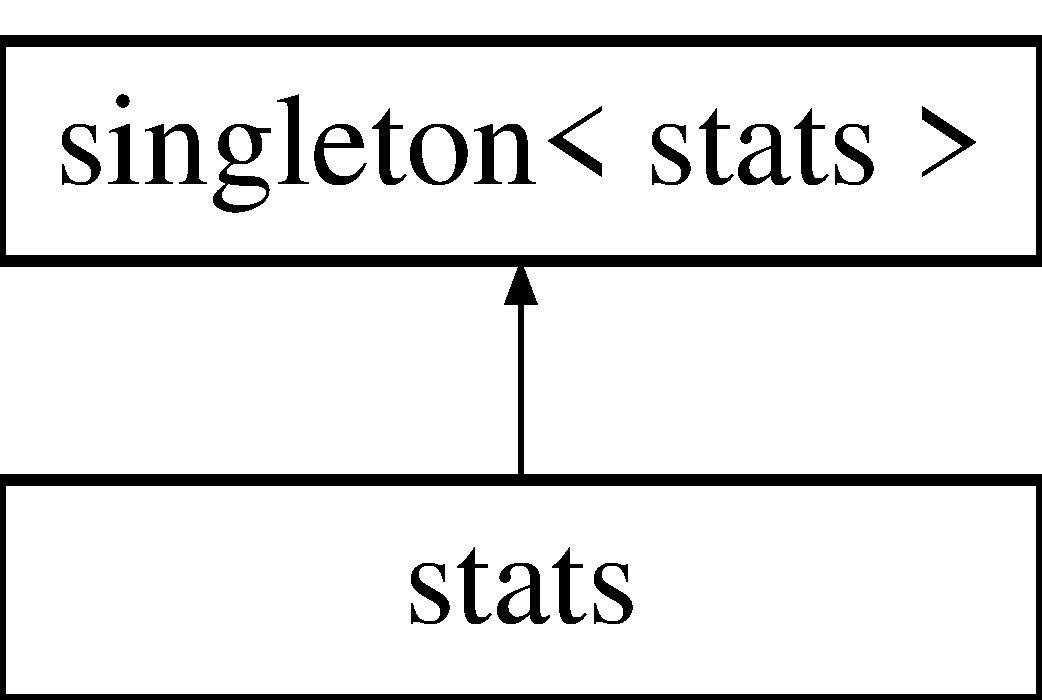
\includegraphics[height=2cm]{classstats}
\end{center}
\end{figure}
\subsection*{Classes}
\begin{CompactItemize}
\item 
class \textbf{scoped\_\-read\_\-timer}
\item 
class \textbf{scoped\_\-wait\_\-timer}
\item 
class \textbf{scoped\_\-write\_\-timer}
\end{CompactItemize}
\subsection*{Public Member Functions}
\begin{CompactItemize}
\item 
unsigned \hyperlink{group__iolayer_g6263716c232b9ebe0936f34fd25dd8d4}{get\_\-reads} () const 
\begin{CompactList}\small\item\em Returns total number of reads. \item\end{CompactList}\item 
unsigned \hyperlink{group__iolayer_gf75ae32372c803dcf31e58b0a5e312e2}{get\_\-writes} () const 
\begin{CompactList}\small\item\em Returns total number of writes. \item\end{CompactList}\item 
int64\_\-t \hyperlink{group__iolayer_g32d9c7436d0728f59ce53c269484ced3}{get\_\-read\_\-volume} () const 
\begin{CompactList}\small\item\em Returns number of bytes read from disks. \item\end{CompactList}\item 
int64\_\-t \hyperlink{group__iolayer_g29a2dd5f32d956bae0b02503ac7d0876}{get\_\-written\_\-volume} () const 
\begin{CompactList}\small\item\em Returns number of bytes written to the disks. \item\end{CompactList}\item 
double \hyperlink{group__iolayer_g5425890c2062eb9bed6a73343b8ffb25}{get\_\-read\_\-time} () const 
\begin{CompactList}\small\item\em Time that would be spent in read syscalls if all parallel reads were serialized. \item\end{CompactList}\item 
double \hyperlink{group__iolayer_g38c56edfce29a67fc2312dd2d012caaa}{get\_\-write\_\-time} () const 
\begin{CompactList}\small\item\em Time that would be spent in write syscalls if all parallel writes were serialized. \item\end{CompactList}\item 
double \hyperlink{group__iolayer_g8dce58f17e3ef7d8465b097a72f0a781}{get\_\-pread\_\-time} () const 
\begin{CompactList}\small\item\em Period of time when at least one I/O thread was executing a read. \item\end{CompactList}\item 
double \hyperlink{group__iolayer_gd9f7e56d99697abdca76f1ef1ea1ff00}{get\_\-pwrite\_\-time} () const 
\begin{CompactList}\small\item\em Period of time when at least one I/O thread was executing a write. \item\end{CompactList}\item 
double \hyperlink{group__iolayer_g70efd6899577c26be66ad527c6776c44}{get\_\-pio\_\-time} () const 
\begin{CompactList}\small\item\em Period of time when at least one I/O thread was executing a read or a write. \item\end{CompactList}\item 
double \hyperlink{group__iolayer_gfb84d41b01e495224d1e0033386ee55c}{get\_\-io\_\-wait\_\-time} () const 
\begin{CompactList}\small\item\em I/O wait time counter. \item\end{CompactList}\item 
double \hyperlink{group__iolayer_g536af25232d9f9f65e64fbf480b37846}{get\_\-last\_\-reset\_\-time} () const 
\begin{CompactList}\small\item\em Return time of the last reset. \item\end{CompactList}\item 
\hypertarget{group__iolayer_g4b34c969ba2786ae1c29eb01708c2572}{
void \hyperlink{group__iolayer_g4b34c969ba2786ae1c29eb01708c2572}{reset} ()}
\label{group__iolayer_g4b34c969ba2786ae1c29eb01708c2572}

\begin{CompactList}\small\item\em Resets I/O time counters (including I/O wait counter). \item\end{CompactList}\item 
\hypertarget{group__iolayer_gf87dff3952823db0588ead65b2af0b3f}{
void \textbf{write\_\-started} (unsigned size\_\-)}
\label{group__iolayer_gf87dff3952823db0588ead65b2af0b3f}

\item 
\hypertarget{group__iolayer_g5965fa84c7858b4ca62498106ffdb09b}{
void \textbf{write\_\-finished} ()}
\label{group__iolayer_g5965fa84c7858b4ca62498106ffdb09b}

\item 
\hypertarget{group__iolayer_gafaf899b318946ab046da27c93ef49e4}{
void \textbf{read\_\-started} (unsigned size\_\-)}
\label{group__iolayer_gafaf899b318946ab046da27c93ef49e4}

\item 
\hypertarget{group__iolayer_g0c21c9569c80c2708b9930971502ed4f}{
void \textbf{read\_\-finished} ()}
\label{group__iolayer_g0c21c9569c80c2708b9930971502ed4f}

\item 
\hypertarget{group__iolayer_g6fd33395eeac6ec8929b930e4fef328a}{
void \textbf{wait\_\-started} ()}
\label{group__iolayer_g6fd33395eeac6ec8929b930e4fef328a}

\item 
\hypertarget{group__iolayer_g98c7d5499874405c7688519c8d328f93}{
void \textbf{wait\_\-finished} ()}
\label{group__iolayer_g98c7d5499874405c7688519c8d328f93}

\end{CompactItemize}
\subsection*{Friends}
\begin{CompactItemize}
\item 
\hypertarget{classstats_22b8478672f97fdf6efe2991e6d3a906}{
class \textbf{singleton$<$ stats $>$}}
\label{classstats_22b8478672f97fdf6efe2991e6d3a906}

\end{CompactItemize}


\subsection{Detailed Description}
Collects various I/O statistics. 

\begin{Desc}
\item[Remarks:]is a singleton \end{Desc}


Definition at line 49 of file iostats.h.

The documentation for this class was generated from the following file:\begin{CompactItemize}
\item 
/home/Kevin/izenelib/include/am/blockmanager/iostats.h\end{CompactItemize}

\hypertarget{classtc__hash}{
\section{tc\_\-hash$<$ KeyType, ValueType, LockType $>$ Class Template Reference}
\label{classtc__hash}\index{tc\_\-hash@{tc\_\-hash}}
}
wrap tokyo/cabinet for CacheDB and SDB.  


{\tt \#include $<$tc\_\-hash.h$>$}

Inheritance diagram for tc\_\-hash$<$ KeyType, ValueType, LockType $>$::\begin{figure}[H]
\begin{center}
\leavevmode
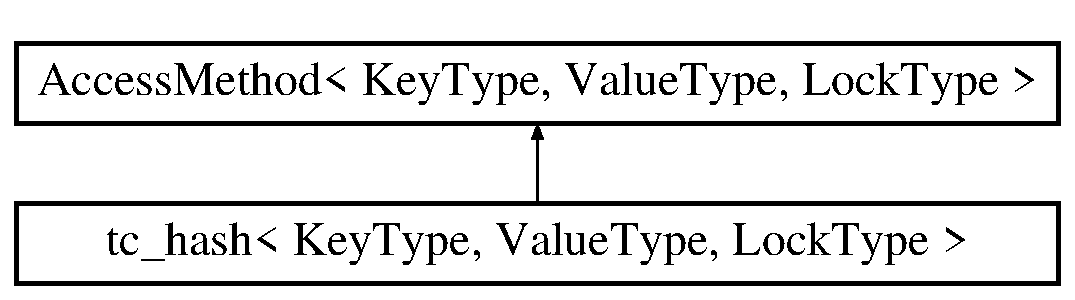
\includegraphics[height=2cm]{classtc__hash}
\end{center}
\end{figure}
\subsection*{Public Types}
\begin{CompactItemize}
\item 
\hypertarget{classtc__hash_372762dbf429e556715eb2893f395ac4}{
typedef KeyType \textbf{SDBCursor}}
\label{classtc__hash_372762dbf429e556715eb2893f395ac4}

\item 
\hypertarget{classtc__hash_f7211ed16f32c7b57b6ba567ae141eed}{
typedef DataType$<$ KeyType, ValueType $>$ \textbf{DataType}}
\label{classtc__hash_f7211ed16f32c7b57b6ba567ae141eed}

\end{CompactItemize}
\subsection*{Public Member Functions}
\begin{CompactItemize}
\item 
\hyperlink{classtc__hash_f65eca712c3a612bb1ce1defa865659f}{tc\_\-hash} (const string \&fileName=\char`\"{}tc\_\-hash.dat\char`\"{})
\item 
virtual \hyperlink{classtc__hash_1f9a677246db4a5a14be9fb7a5b3547b}{$\sim$tc\_\-hash} ()
\item 
void \hyperlink{classtc__hash_95514cd1ac7f01332038973d0c8db323}{setCacheSize} (size\_\-t cacheSize)
\item 
\hypertarget{classtc__hash_2061749cebcb6e13d1ed08b807b9f2f4}{
std::string \hyperlink{classtc__hash_2061749cebcb6e13d1ed08b807b9f2f4}{getFileName} () const }
\label{classtc__hash_2061749cebcb6e13d1ed08b807b9f2f4}

\begin{CompactList}\small\item\em return the \hyperlink{classfile}{file} name of the SequentialDB \item\end{CompactList}\item 
bool \hyperlink{classtc__hash_dec46db22458aace6d4c384d0136f73a}{insert} (const DataType \&dat)
\item 
bool \hyperlink{classtc__hash_a0f14b10040effe879ba2deb5c0a961b}{insert} (const KeyType \&key, const ValueType \&value)
\item 
ValueType $\ast$ \hyperlink{classtc__hash_f6288e85c3973f121c25a39c0cab55ec}{find} (const KeyType \&key)
\item 
\hypertarget{classtc__hash_89cb493b5270be235141cd5131806e10}{
bool \textbf{get} (const KeyType \&key, ValueType \&value)}
\label{classtc__hash_89cb493b5270be235141cd5131806e10}

\item 
bool \hyperlink{classtc__hash_ace3bd9142e9e66ca01aa0de990d145e}{del} (const KeyType \&key)
\item 
bool \hyperlink{classtc__hash_d9f9b4ea4cf3424ca2112bb1ba9293f2}{update} (const DataType \&dat)
\item 
bool \hyperlink{classtc__hash_2aa23c6cb581dae26a9bf2f98e313f00}{update} (const KeyType \&key, const ValueType \&value)
\item 
SDBCursor \hyperlink{classtc__hash_996ea5e3297bcbce4c6a7a0ca8e17d21}{search} (const KeyType \&key)
\item 
bool \hyperlink{classtc__hash_57246a88334c225644111bbf0a127e8e}{search} (const KeyType \&key, SDBCursor \&locn)
\item 
SDBCursor \hyperlink{classtc__hash_3c7efb056e568de793b82a30c66f9640}{get\_\-first\_\-locn} ()
\item 
\hypertarget{classtc__hash_e8d97949604477ba8f6b59ce3d3e976f}{
bool \textbf{get} (const SDBCursor \&locn, KeyType \&key, ValueType \&value)}
\label{classtc__hash_e8d97949604477ba8f6b59ce3d3e976f}

\item 
bool \hyperlink{classtc__hash_43f0d4a9a0ceda515d782000b81928c3}{get} (const SDBCursor \&locn, DataType \&rec)
\item 
bool \hyperlink{classtc__hash_25d62cc64ce4c777c279101dca5aa846}{seq} (SDBCursor \&locn, DataType \&rec, ESeqDirection sdir=ESD\_\-FORWARD)
\begin{CompactList}\small\item\em sequential access method \item\end{CompactList}\item 
int \hyperlink{classtc__hash_51837772025d390b3a9b1c87ec15309d}{num\_\-items} ()
\item 
bool \hyperlink{classtc__hash_782627d77d2ef0bab952c38992c5c743}{open} ()
\item 
bool \hyperlink{classtc__hash_8153ff6485a0382fac5b5a20c0cc9033}{close} ()
\item 
void \hyperlink{classtc__hash_83474cdc095650dfea677f3b65aaa032}{commit} ()
\item 
void \hyperlink{classtc__hash_3ffb4206aed13ea94ff623cc46d971da}{flush} ()
\item 
void \hyperlink{classtc__hash_b29bf2580a2dc3b10497ea920bf98f00}{display} (std::ostream \&os=std::cout)
\item 
TCHDB $\ast$ \hyperlink{classtc__hash_ab77b561b8897ccdca73515233493f7a}{getHandle} ()
\end{CompactItemize}


\subsection{Detailed Description}
\subsubsection*{template$<$typename KeyType, typename ValueType, typename LockType = NullLock$>$ class tc\_\-hash$<$ KeyType, ValueType, LockType $>$}

wrap tokyo/cabinet for CacheDB and SDB. 

Definition at line 22 of file tc\_\-hash.h.

\subsection{Constructor \& Destructor Documentation}
\hypertarget{classtc__hash_f65eca712c3a612bb1ce1defa865659f}{
\index{tc\_\-hash@{tc\_\-hash}!tc\_\-hash@{tc\_\-hash}}
\index{tc\_\-hash@{tc\_\-hash}!tc_hash@{tc\_\-hash}}
\subsubsection[{tc\_\-hash}]{\setlength{\rightskip}{0pt plus 5cm}template$<$typename KeyType , typename ValueType , typename LockType  = NullLock$>$ {\bf tc\_\-hash}$<$ KeyType, ValueType, LockType $>$::{\bf tc\_\-hash} (const string \& {\em fileName} = {\tt \char`\"{}tc\_\-hash$<$~KeyType,~ValueType,~LockType~$>$.dat\char`\"{}})\hspace{0.3cm}{\tt  \mbox{[}inline\mbox{]}}}}
\label{classtc__hash_f65eca712c3a612bb1ce1defa865659f}


constructor 

Definition at line 32 of file tc\_\-hash.h.\hypertarget{classtc__hash_1f9a677246db4a5a14be9fb7a5b3547b}{
\index{tc\_\-hash@{tc\_\-hash}!$\sim$tc\_\-hash@{$\sim$tc\_\-hash}}
\index{$\sim$tc\_\-hash@{$\sim$tc\_\-hash}!tc_hash@{tc\_\-hash}}
\subsubsection[{$\sim$tc\_\-hash}]{\setlength{\rightskip}{0pt plus 5cm}template$<$typename KeyType , typename ValueType , typename LockType  = NullLock$>$ virtual {\bf tc\_\-hash}$<$ KeyType, ValueType, LockType $>$::$\sim${\bf tc\_\-hash} ()\hspace{0.3cm}{\tt  \mbox{[}inline, virtual\mbox{]}}}}
\label{classtc__hash_1f9a677246db4a5a14be9fb7a5b3547b}


deconstructor, \hyperlink{classtc__hash_8153ff6485a0382fac5b5a20c0cc9033}{close()} will also be called here. 

Definition at line 38 of file tc\_\-hash.h.

\subsection{Member Function Documentation}
\hypertarget{classtc__hash_8153ff6485a0382fac5b5a20c0cc9033}{
\index{tc\_\-hash@{tc\_\-hash}!close@{close}}
\index{close@{close}!tc_hash@{tc\_\-hash}}
\subsubsection[{close}]{\setlength{\rightskip}{0pt plus 5cm}template$<$typename KeyType , typename ValueType , typename LockType  = NullLock$>$ bool {\bf tc\_\-hash}$<$ KeyType, ValueType, LockType $>$::close ()\hspace{0.3cm}{\tt  \mbox{[}inline\mbox{]}}}}
\label{classtc__hash_8153ff6485a0382fac5b5a20c0cc9033}


db should be closed after open, and it will automatically called in deconstuctor. 

Definition at line 274 of file tc\_\-hash.h.\hypertarget{classtc__hash_83474cdc095650dfea677f3b65aaa032}{
\index{tc\_\-hash@{tc\_\-hash}!commit@{commit}}
\index{commit@{commit}!tc_hash@{tc\_\-hash}}
\subsubsection[{commit}]{\setlength{\rightskip}{0pt plus 5cm}template$<$typename KeyType , typename ValueType , typename LockType  = NullLock$>$ void {\bf tc\_\-hash}$<$ KeyType, ValueType, LockType $>$::commit ()\hspace{0.3cm}{\tt  \mbox{[}inline\mbox{]}}}}
\label{classtc__hash_83474cdc095650dfea677f3b65aaa032}


write the dirty buckets to disk, not release the memory 

Definition at line 284 of file tc\_\-hash.h.\hypertarget{classtc__hash_ace3bd9142e9e66ca01aa0de990d145e}{
\index{tc\_\-hash@{tc\_\-hash}!del@{del}}
\index{del@{del}!tc_hash@{tc\_\-hash}}
\subsubsection[{del}]{\setlength{\rightskip}{0pt plus 5cm}template$<$typename KeyType , typename ValueType , typename LockType  = NullLock$>$ bool {\bf tc\_\-hash}$<$ KeyType, ValueType, LockType $>$::del (const KeyType \& {\em key})\hspace{0.3cm}{\tt  \mbox{[}inline\mbox{]}}}}
\label{classtc__hash_ace3bd9142e9e66ca01aa0de990d145e}


delete an item 

Definition at line 126 of file tc\_\-hash.h.\hypertarget{classtc__hash_b29bf2580a2dc3b10497ea920bf98f00}{
\index{tc\_\-hash@{tc\_\-hash}!display@{display}}
\index{display@{display}!tc_hash@{tc\_\-hash}}
\subsubsection[{display}]{\setlength{\rightskip}{0pt plus 5cm}template$<$typename KeyType , typename ValueType , typename LockType  = NullLock$>$ void {\bf tc\_\-hash}$<$ KeyType, ValueType, LockType $>$::display (std::ostream \& {\em os} = {\tt std::cout})\hspace{0.3cm}{\tt  \mbox{[}inline\mbox{]}}}}
\label{classtc__hash_b29bf2580a2dc3b10497ea920bf98f00}


display the info of \hyperlink{classtc__hash}{tc\_\-hash} 

Definition at line 297 of file tc\_\-hash.h.\hypertarget{classtc__hash_f6288e85c3973f121c25a39c0cab55ec}{
\index{tc\_\-hash@{tc\_\-hash}!find@{find}}
\index{find@{find}!tc_hash@{tc\_\-hash}}
\subsubsection[{find}]{\setlength{\rightskip}{0pt plus 5cm}template$<$typename KeyType , typename ValueType , typename LockType  = NullLock$>$ ValueType$\ast$ {\bf tc\_\-hash}$<$ KeyType, ValueType, LockType $>$::find (const KeyType \& {\em key})\hspace{0.3cm}{\tt  \mbox{[}inline\mbox{]}}}}
\label{classtc__hash_f6288e85c3973f121c25a39c0cab55ec}


find an item, return pointer to the value. Note that, there will be memory leak if not delete the value 

Definition at line 86 of file tc\_\-hash.h.\hypertarget{classtc__hash_3ffb4206aed13ea94ff623cc46d971da}{
\index{tc\_\-hash@{tc\_\-hash}!flush@{flush}}
\index{flush@{flush}!tc_hash@{tc\_\-hash}}
\subsubsection[{flush}]{\setlength{\rightskip}{0pt plus 5cm}template$<$typename KeyType , typename ValueType , typename LockType  = NullLock$>$ void {\bf tc\_\-hash}$<$ KeyType, ValueType, LockType $>$::flush ()\hspace{0.3cm}{\tt  \mbox{[}inline\mbox{]}}}}
\label{classtc__hash_3ffb4206aed13ea94ff623cc46d971da}


Write the dirty buckets to disk and also free up most of the memory. Note that, for efficieny, entry\_\-\mbox{[}\mbox{]} is not freed up. 

Definition at line 291 of file tc\_\-hash.h.\hypertarget{classtc__hash_43f0d4a9a0ceda515d782000b81928c3}{
\index{tc\_\-hash@{tc\_\-hash}!get@{get}}
\index{get@{get}!tc_hash@{tc\_\-hash}}
\subsubsection[{get}]{\setlength{\rightskip}{0pt plus 5cm}template$<$typename KeyType , typename ValueType , typename LockType  = NullLock$>$ bool {\bf tc\_\-hash}$<$ KeyType, ValueType, LockType $>$::get (const SDBCursor \& {\em locn}, \/  DataType \& {\em rec})\hspace{0.3cm}{\tt  \mbox{[}inline\mbox{]}}}}
\label{classtc__hash_43f0d4a9a0ceda515d782000b81928c3}


get an item from given SDBCursor 

Definition at line 214 of file tc\_\-hash.h.\hypertarget{classtc__hash_3c7efb056e568de793b82a30c66f9640}{
\index{tc\_\-hash@{tc\_\-hash}!get\_\-first\_\-locn@{get\_\-first\_\-locn}}
\index{get\_\-first\_\-locn@{get\_\-first\_\-locn}!tc_hash@{tc\_\-hash}}
\subsubsection[{get\_\-first\_\-locn}]{\setlength{\rightskip}{0pt plus 5cm}template$<$typename KeyType , typename ValueType , typename LockType  = NullLock$>$ SDBCursor {\bf tc\_\-hash}$<$ KeyType, ValueType, LockType $>$::get\_\-first\_\-locn ()\hspace{0.3cm}{\tt  \mbox{[}inline\mbox{]}}}}
\label{classtc__hash_3c7efb056e568de793b82a30c66f9640}


get the SDBCursor of first item in the first not empty bucket. 

Definition at line 193 of file tc\_\-hash.h.\hypertarget{classtc__hash_ab77b561b8897ccdca73515233493f7a}{
\index{tc\_\-hash@{tc\_\-hash}!getHandle@{getHandle}}
\index{getHandle@{getHandle}!tc_hash@{tc\_\-hash}}
\subsubsection[{getHandle}]{\setlength{\rightskip}{0pt plus 5cm}template$<$typename KeyType , typename ValueType , typename LockType  = NullLock$>$ TCHDB$\ast$ {\bf tc\_\-hash}$<$ KeyType, ValueType, LockType $>$::getHandle ()\hspace{0.3cm}{\tt  \mbox{[}inline\mbox{]}}}}
\label{classtc__hash_ab77b561b8897ccdca73515233493f7a}


We can directly process hdb\_\- by this handle. 

Definition at line 303 of file tc\_\-hash.h.\hypertarget{classtc__hash_a0f14b10040effe879ba2deb5c0a961b}{
\index{tc\_\-hash@{tc\_\-hash}!insert@{insert}}
\index{insert@{insert}!tc_hash@{tc\_\-hash}}
\subsubsection[{insert}]{\setlength{\rightskip}{0pt plus 5cm}template$<$typename KeyType , typename ValueType , typename LockType  = NullLock$>$ bool {\bf tc\_\-hash}$<$ KeyType, ValueType, LockType $>$::insert (const KeyType \& {\em key}, \/  const ValueType \& {\em value})\hspace{0.3cm}{\tt  \mbox{[}inline\mbox{]}}}}
\label{classtc__hash_a0f14b10040effe879ba2deb5c0a961b}


insert an item in key/value pair 

Definition at line 68 of file tc\_\-hash.h.\hypertarget{classtc__hash_dec46db22458aace6d4c384d0136f73a}{
\index{tc\_\-hash@{tc\_\-hash}!insert@{insert}}
\index{insert@{insert}!tc_hash@{tc\_\-hash}}
\subsubsection[{insert}]{\setlength{\rightskip}{0pt plus 5cm}template$<$typename KeyType , typename ValueType , typename LockType  = NullLock$>$ bool {\bf tc\_\-hash}$<$ KeyType, ValueType, LockType $>$::insert (const DataType \& {\em dat})\hspace{0.3cm}{\tt  \mbox{[}inline\mbox{]}}}}
\label{classtc__hash_dec46db22458aace6d4c384d0136f73a}


insert an item of DataType 

Definition at line 61 of file tc\_\-hash.h.\hypertarget{classtc__hash_51837772025d390b3a9b1c87ec15309d}{
\index{tc\_\-hash@{tc\_\-hash}!num\_\-items@{num\_\-items}}
\index{num\_\-items@{num\_\-items}!tc_hash@{tc\_\-hash}}
\subsubsection[{num\_\-items}]{\setlength{\rightskip}{0pt plus 5cm}template$<$typename KeyType , typename ValueType , typename LockType  = NullLock$>$ int {\bf tc\_\-hash}$<$ KeyType, ValueType, LockType $>$::num\_\-items ()\hspace{0.3cm}{\tt  \mbox{[}inline\mbox{]}}}}
\label{classtc__hash_51837772025d390b3a9b1c87ec15309d}


get the num of items 

Definition at line 259 of file tc\_\-hash.h.\hypertarget{classtc__hash_782627d77d2ef0bab952c38992c5c743}{
\index{tc\_\-hash@{tc\_\-hash}!open@{open}}
\index{open@{open}!tc_hash@{tc\_\-hash}}
\subsubsection[{open}]{\setlength{\rightskip}{0pt plus 5cm}template$<$typename KeyType , typename ValueType , typename LockType  = NullLock$>$ bool {\bf tc\_\-hash}$<$ KeyType, ValueType, LockType $>$::open ()\hspace{0.3cm}{\tt  \mbox{[}inline\mbox{]}}}}
\label{classtc__hash_782627d77d2ef0bab952c38992c5c743}


db must be opened to be used. 

Definition at line 267 of file tc\_\-hash.h.\hypertarget{classtc__hash_57246a88334c225644111bbf0a127e8e}{
\index{tc\_\-hash@{tc\_\-hash}!search@{search}}
\index{search@{search}!tc_hash@{tc\_\-hash}}
\subsubsection[{search}]{\setlength{\rightskip}{0pt plus 5cm}template$<$typename KeyType , typename ValueType , typename LockType  = NullLock$>$ bool {\bf tc\_\-hash}$<$ KeyType, ValueType, LockType $>$::search (const KeyType \& {\em key}, \/  SDBCursor \& {\em locn})\hspace{0.3cm}{\tt  \mbox{[}inline\mbox{]}}}}
\label{classtc__hash_57246a88334c225644111bbf0a127e8e}


another search function, flushCache\_\-() will be called at the beginning, 

Definition at line 180 of file tc\_\-hash.h.\hypertarget{classtc__hash_996ea5e3297bcbce4c6a7a0ca8e17d21}{
\index{tc\_\-hash@{tc\_\-hash}!search@{search}}
\index{search@{search}!tc_hash@{tc\_\-hash}}
\subsubsection[{search}]{\setlength{\rightskip}{0pt plus 5cm}template$<$typename KeyType , typename ValueType , typename LockType  = NullLock$>$ SDBCursor {\bf tc\_\-hash}$<$ KeyType, ValueType, LockType $>$::search (const KeyType \& {\em key})\hspace{0.3cm}{\tt  \mbox{[}inline\mbox{]}}}}
\label{classtc__hash_996ea5e3297bcbce4c6a7a0ca8e17d21}


search an item

\begin{Desc}
\item[Returns:]SDBCursor \end{Desc}


Definition at line 166 of file tc\_\-hash.h.\hypertarget{classtc__hash_25d62cc64ce4c777c279101dca5aa846}{
\index{tc\_\-hash@{tc\_\-hash}!seq@{seq}}
\index{seq@{seq}!tc_hash@{tc\_\-hash}}
\subsubsection[{seq}]{\setlength{\rightskip}{0pt plus 5cm}template$<$typename KeyType , typename ValueType , typename LockType  = NullLock$>$ bool {\bf tc\_\-hash}$<$ KeyType, ValueType, LockType $>$::seq (SDBCursor \& {\em locn}, \/  DataType \& {\em rec}, \/  ESeqDirection {\em sdir} = {\tt ESD\_\-FORWARD})\hspace{0.3cm}{\tt  \mbox{[}inline\mbox{]}}}}
\label{classtc__hash_25d62cc64ce4c777c279101dca5aa846}


sequential access method 

\begin{Desc}
\item[Parameters:]
\begin{description}
\item[{\em locn}]is the current SDBCursor, and will replaced next SDBCursor when route finished. \item[{\em rec}]is the item in SDBCursor locn. \item[{\em sdir}]is sequential access direction, for hash is unordered, we only implement forward case. \end{description}
\end{Desc}


Definition at line 226 of file tc\_\-hash.h.\hypertarget{classtc__hash_95514cd1ac7f01332038973d0c8db323}{
\index{tc\_\-hash@{tc\_\-hash}!setCacheSize@{setCacheSize}}
\index{setCacheSize@{setCacheSize}!tc_hash@{tc\_\-hash}}
\subsubsection[{setCacheSize}]{\setlength{\rightskip}{0pt plus 5cm}template$<$typename KeyType , typename ValueType , typename LockType  = NullLock$>$ void {\bf tc\_\-hash}$<$ KeyType, ValueType, LockType $>$::setCacheSize (size\_\-t {\em cacheSize})\hspace{0.3cm}{\tt  \mbox{[}inline\mbox{]}}}}
\label{classtc__hash_95514cd1ac7f01332038973d0c8db323}


set cache size, if not called use default size 100000 

Definition at line 46 of file tc\_\-hash.h.\hypertarget{classtc__hash_2aa23c6cb581dae26a9bf2f98e313f00}{
\index{tc\_\-hash@{tc\_\-hash}!update@{update}}
\index{update@{update}!tc_hash@{tc\_\-hash}}
\subsubsection[{update}]{\setlength{\rightskip}{0pt plus 5cm}template$<$typename KeyType , typename ValueType , typename LockType  = NullLock$>$ bool {\bf tc\_\-hash}$<$ KeyType, ValueType, LockType $>$::update (const KeyType \& {\em key}, \/  const ValueType \& {\em value})\hspace{0.3cm}{\tt  \mbox{[}inline\mbox{]}}}}
\label{classtc__hash_2aa23c6cb581dae26a9bf2f98e313f00}


update an item by key/value pair 

Definition at line 147 of file tc\_\-hash.h.\hypertarget{classtc__hash_d9f9b4ea4cf3424ca2112bb1ba9293f2}{
\index{tc\_\-hash@{tc\_\-hash}!update@{update}}
\index{update@{update}!tc_hash@{tc\_\-hash}}
\subsubsection[{update}]{\setlength{\rightskip}{0pt plus 5cm}template$<$typename KeyType , typename ValueType , typename LockType  = NullLock$>$ bool {\bf tc\_\-hash}$<$ KeyType, ValueType, LockType $>$::update (const DataType \& {\em dat})\hspace{0.3cm}{\tt  \mbox{[}inline\mbox{]}}}}
\label{classtc__hash_d9f9b4ea4cf3424ca2112bb1ba9293f2}


update an item through DataType data 

Definition at line 139 of file tc\_\-hash.h.

The documentation for this class was generated from the following file:\begin{CompactItemize}
\item 
/home/Kevin/izenelib/include/am/tokyo\_\-cabinet/\hyperlink{tc__hash_8h}{tc\_\-hash.h}\end{CompactItemize}

\hypertarget{classtyped__block}{
\section{typed\_\-block$<$ RawSize\_\-, T\_\-, NRef\_\-, InfoType\_\- $>$ Class Template Reference}
\label{classtyped__block}\index{typed\_\-block@{typed\_\-block}}
}
Block containing elements of fixed length.  


{\tt \#include $<$main.h$>$}

Inheritance diagram for typed\_\-block$<$ RawSize\_\-, T\_\-, NRef\_\-, InfoType\_\- $>$::\begin{figure}[H]
\begin{center}
\leavevmode
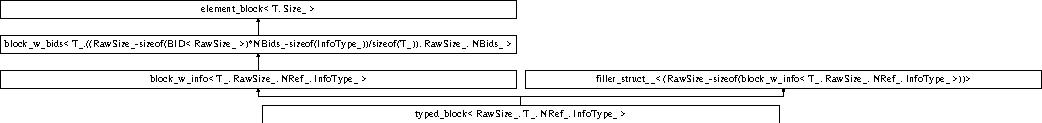
\includegraphics[height=1.64948cm]{classtyped__block}
\end{center}
\end{figure}
\subsection*{Public Types}
\begin{CompactItemize}
\item 
enum \{ \textbf{has\_\-filler} =  (RawSize\_\- != sizeof(block\_\-w\_\-info$<$T\_\-, RawSize\_\-, NRef\_\-, InfoType\_\-$>$))
 \}
\item 
enum \{ \par
\hyperlink{group__mnglayer_gg43854e49708cf32d97e65d727593833c53f1c9c4e116e026d8096110c42f27ea}{raw\_\-size} =  RawSize\_\-, 
\hyperlink{group__mnglayer_gg43854e49708cf32d97e65d727593833c8e272a078e257c8700b765dc85bf53a2}{size} =  block\_\-w\_\-info$<$T\_\-, 
\textbf{RawSize\_\-}, 
\textbf{NRef\_\-}, 
\par
\hyperlink{group__mnglayer_gg43854e49708cf32d97e65d727593833c8e272a078e257c8700b765dc85bf53a2}{size} =  block\_\-w\_\-info$<$T\_\-
 \}
\item 
\hypertarget{classtyped__block_743585b8b2228c06af23f996e03c0110}{
typedef T\_\- \textbf{type}}
\label{classtyped__block_743585b8b2228c06af23f996e03c0110}

\item 
\hypertarget{group__mnglayer_g7f42e0c3e742cf3733e0d5592d54ab58}{
typedef T\_\- \textbf{value\_\-type}}
\label{group__mnglayer_g7f42e0c3e742cf3733e0d5592d54ab58}

\item 
\hypertarget{group__mnglayer_g521aff2a3700245029372deb0be2b287}{
typedef T\_\- \& \textbf{reference}}
\label{group__mnglayer_g521aff2a3700245029372deb0be2b287}

\item 
\hypertarget{group__mnglayer_g34e897ac51826913281aaf4b10465659}{
typedef const T\_\- \& \textbf{const\_\-reference}}
\label{group__mnglayer_g34e897ac51826913281aaf4b10465659}

\item 
\hypertarget{group__mnglayer_gbc7c8a98ff603c8087eb1fd8974ea270}{
typedef type $\ast$ \textbf{pointer}}
\label{group__mnglayer_gbc7c8a98ff603c8087eb1fd8974ea270}

\item 
\hypertarget{group__mnglayer_g75bd38227d7b7e5b772911ab87d0e7bc}{
typedef pointer \textbf{iterator}}
\label{group__mnglayer_g75bd38227d7b7e5b772911ab87d0e7bc}

\item 
\hypertarget{group__mnglayer_g7cbb990a4e44249df63a9e878aec6338}{
typedef type const $\ast$ \textbf{const\_\-iterator}}
\label{group__mnglayer_g7cbb990a4e44249df63a9e878aec6338}

\item 
\hypertarget{group__mnglayer_gae0703379ce10cdd001a53c8983bbdf5}{
typedef \hyperlink{structBID}{BID}$<$ RawSize\_\- $>$ \textbf{bid\_\-type}}
\label{group__mnglayer_gae0703379ce10cdd001a53c8983bbdf5}

\end{CompactItemize}
\subsection*{Public Member Functions}
\begin{CompactItemize}
\item 
\hyperlink{classrequest__ptr}{request\_\-ptr} \hyperlink{group__mnglayer_gc9c8caa89ae04a3b8dc3d1793eda61b0}{write} (const \hyperlink{structBID}{BID}$<$ raw\_\-size $>$ \&bid, \hyperlink{classcompletion__handler}{completion\_\-handler} on\_\-cmpl=\hyperlink{structdefault__completion__handler}{default\_\-completion\_\-handler}())
\begin{CompactList}\small\item\em Writes block to the disk(s) ! \item\end{CompactList}\item 
\hyperlink{classrequest__ptr}{request\_\-ptr} \hyperlink{group__mnglayer_ge5f58b3358b383d44832ce0fbef7e015}{read} (const \hyperlink{structBID}{BID}$<$ raw\_\-size $>$ \&bid, \hyperlink{classcompletion__handler}{completion\_\-handler} on\_\-cmpl=\hyperlink{structdefault__completion__handler}{default\_\-completion\_\-handler}())
\begin{CompactList}\small\item\em Reads block from the disk(s) ! \item\end{CompactList}\end{CompactItemize}
\subsection*{Static Public Member Functions}
\begin{CompactItemize}
\item 
\hypertarget{group__mnglayer_gfb2c22d3b5ab3c33b98bc3fd71b4b940}{
static void $\ast$ \textbf{operator new\mbox{[}$\,$\mbox{]}} (size\_\-t bytes)}
\label{group__mnglayer_gfb2c22d3b5ab3c33b98bc3fd71b4b940}

\item 
\hypertarget{group__mnglayer_gf322e446d29d36fe3e8687bff69bbd21}{
static void $\ast$ \textbf{operator new} (size\_\-t bytes)}
\label{group__mnglayer_gf322e446d29d36fe3e8687bff69bbd21}

\item 
\hypertarget{group__mnglayer_g46a01a83f3954057c367a23a1e4f0e02}{
static void $\ast$ \textbf{operator new} (size\_\-t, void $\ast$ptr)}
\label{group__mnglayer_g46a01a83f3954057c367a23a1e4f0e02}

\item 
\hypertarget{group__mnglayer_g8c64f56092ff568bad31293b1ccdab53}{
static void \textbf{operator delete\mbox{[}$\,$\mbox{]}} (void $\ast$ptr)}
\label{group__mnglayer_g8c64f56092ff568bad31293b1ccdab53}

\item 
\hypertarget{group__mnglayer_g6c881aecb0a7b2e3c306c3d47e846140}{
static void \textbf{operator delete} (void $\ast$ptr)}
\label{group__mnglayer_g6c881aecb0a7b2e3c306c3d47e846140}

\item 
\hypertarget{group__mnglayer_gcaec0a5f3e2d6ff44e1d7fa30ff602b5}{
static void \textbf{operator delete} (void $\ast$, void $\ast$)}
\label{group__mnglayer_gcaec0a5f3e2d6ff44e1d7fa30ff602b5}

\end{CompactItemize}


\subsection{Detailed Description}
\subsubsection*{template$<$unsigned RawSize\_\-, class T\_\-, unsigned NRef\_\- = 0, class InfoType\_\- = void$>$ class typed\_\-block$<$ RawSize\_\-, T\_\-, NRef\_\-, InfoType\_\- $>$}

Block containing elements of fixed length. 

Template parameters:\begin{itemize}
\item {\tt RawSize\_\-} size of block in bytes\item {\tt T\_\-} type of block's records\item {\tt NRef\_\-} number of block references (BIDs) that can be stored in the block (default is 0)\item {\tt InfoType\_\-} type of per block information (default is no information - void)\end{itemize}


The data array of type T\_\- is contained in the parent class {\tt \hyperlink{classelement__block}{element\_\-block}}, see related information there. The \hyperlink{structBID}{BID} array of references is contained in the parent class {\tt \hyperlink{classblock__w__bids}{block\_\-w\_\-bids}}, see related information there. The \char`\"{}per block information\char`\"{} is contained in the parent class {\tt \hyperlink{classblock__w__info}{block\_\-w\_\-info}}, see related information there. \begin{Desc}
\item[Warning:]If {\tt RawSize\_\-} $>$ 2MB object(s) of this type can not be allocated on the stack (as a function variable for example), because Linux POSIX library limits the stack size for the main thread to (2MB - system page size) \end{Desc}


Definition at line 290 of file main.h.

The documentation for this class was generated from the following file:\begin{CompactItemize}
\item 
/home/Kevin/izenelib/include/am/blockmanager/main.h\end{CompactItemize}

\chapter{File Documentation}
\hypertarget{LinearHashTable_8h}{
\section{/home/Kevin/izenelib/include/am/fromylib/LinearHashTable.h File Reference}
\label{LinearHashTable_8h}\index{/home/Kevin/izenelib/include/am/fromylib/LinearHashTable.h@{/home/Kevin/izenelib/include/am/fromylib/LinearHashTable.h}}
}
The header \hyperlink{classfile}{file} of definition of linear hashing table based on memory.  


{\tt \#include \char`\"{}ylib\_\-basics.h\char`\"{}}\par
\subsection*{Classes}
\begin{CompactItemize}
\item 
class \textbf{LHTElem$<$ DataType $>$}
\item 
class \textbf{Segment$<$ DataType $>$}
\item 
class \hyperlink{classLinearHashTable}{LinearHashTable$<$ KeyType, ValueType, LockType $>$}
\begin{CompactList}\small\item\em \hyperlink{classLinearHashTable}{LinearHashTable} is based on Per-Ake Larson's work, Dynamic Hash Tables. \item\end{CompactList}\end{CompactItemize}
\subsection*{Defines}
\begin{CompactItemize}
\item 
\hypertarget{LinearHashTable_8h_ff9a8c3ba7555a555122439caf7e3184}{
\#define \textbf{LinearHashTable\_\-h}~1}
\label{LinearHashTable_8h_ff9a8c3ba7555a555122439caf7e3184}

\end{CompactItemize}
\subsection*{Functions}
\begin{CompactItemize}
\item 
\hypertarget{LinearHashTable_8h_94fce979b5ed5d0d2a2012e036c55123}{
{\footnotesize template$<$typename KeyType , typename ValueType , typename LockType $>$ }\\std::ostream \& \textbf{operator$<$$<$} (std::ostream \&strm, const \hyperlink{classLinearHashTable}{LinearHashTable}$<$ KeyType, ValueType, LockType $>$ \&src)}
\label{LinearHashTable_8h_94fce979b5ed5d0d2a2012e036c55123}

\end{CompactItemize}
\subsection*{Variables}
\begin{CompactItemize}
\item 
\hypertarget{LinearHashTable_8h_e8b042b29a6326b68249599fd8c4865f}{
NS\_\-IZENELIB\_\-AM\_\-BEGIN class LHTElem \textbf{NS\_\-IZENELIB\_\-AM\_\-END}}
\label{LinearHashTable_8h_e8b042b29a6326b68249599fd8c4865f}

\end{CompactItemize}


\subsection{Detailed Description}
The header \hyperlink{classfile}{file} of definition of linear hashing table based on memory. 



Definition in file \hyperlink{LinearHashTable_8h-source}{LinearHashTable.h}.
\hypertarget{sdb__btree_8h}{
\section{/home/Kevin/izenelib/include/am/sdb\_\-btree/sdb\_\-btree.h File Reference}
\label{sdb__btree_8h}\index{/home/Kevin/izenelib/include/am/sdb\_\-btree/sdb\_\-btree.h@{/home/Kevin/izenelib/include/am/sdb\_\-btree/sdb\_\-btree.h}}
}
The header \hyperlink{classfile}{file} of \hyperlink{classsdb__btree}{sdb\_\-btree}.  


{\tt \#include \char`\"{}sdb\_\-node.h\char`\"{}}\par
\subsection*{Classes}
\begin{CompactItemize}
\item 
class \hyperlink{classsdb__btree}{sdb\_\-btree$<$ KeyType, ValueType, LockType, Alloc $>$}
\begin{CompactList}\small\item\em \hyperlink{classfile}{file} version of cc-b$\ast$-btree \item\end{CompactList}\end{CompactItemize}


\subsection{Detailed Description}
The header \hyperlink{classfile}{file} of \hyperlink{classsdb__btree}{sdb\_\-btree}. 

This \hyperlink{classfile}{file} defines class \hyperlink{classsdb__btree}{sdb\_\-btree}. 

Definition in file \hyperlink{sdb__btree_8h-source}{sdb\_\-btree.h}.
\hypertarget{sdb__btree__header_8h}{
\section{/home/Kevin/izenelib/include/am/sdb\_\-btree/sdb\_\-btree\_\-header.h File Reference}
\label{sdb__btree__header_8h}\index{/home/Kevin/izenelib/include/am/sdb\_\-btree/sdb\_\-btree\_\-header.h@{/home/Kevin/izenelib/include/am/sdb\_\-btree/sdb\_\-btree\_\-header.h}}
}
The header \hyperlink{classfile}{file} of \hyperlink{structCbFileHeader}{CbFileHeader}. This \hyperlink{classfile}{file} defines class \hyperlink{structCbFileHeader}{CbFileHeader}.  


{\tt \#include $<$iostream$>$}\par
{\tt \#include \char`\"{}../../types.h\char`\"{}}\par
\subsection*{Classes}
\begin{CompactItemize}
\item 
struct \hyperlink{structCbFileHeader}{CbFileHeader}
\end{CompactItemize}


\subsection{Detailed Description}
The header \hyperlink{classfile}{file} of \hyperlink{structCbFileHeader}{CbFileHeader}. This \hyperlink{classfile}{file} defines class \hyperlink{structCbFileHeader}{CbFileHeader}. 



Definition in file \hyperlink{sdb__btree__header_8h-source}{sdb\_\-btree\_\-header.h}.
\hypertarget{sdb__node_8h}{
\section{/home/Kevin/izenelib/include/am/sdb\_\-btree/sdb\_\-node.h File Reference}
\label{sdb__node_8h}\index{/home/Kevin/izenelib/include/am/sdb\_\-btree/sdb\_\-node.h@{/home/Kevin/izenelib/include/am/sdb\_\-btree/sdb\_\-node.h}}
}
The header \hyperlink{classfile}{file} of sdb\_\-node.  


{\tt \#include \char`\"{}sdb\_\-btree\_\-types.h\char`\"{}}\par
{\tt \#include \char`\"{}sdb\_\-btree\_\-header.h\char`\"{}}\par
{\tt \#include $<$vector$>$}\par
\subsection*{Typedefs}
\begin{CompactItemize}
\item 
\hypertarget{sdb__node_8h_497086244cdf2dfc4ce6ee8b9f8a382e}{
typedef std::pair$<$ size\_\-t, CChildPos $>$ \textbf{KEYPOS}}
\label{sdb__node_8h_497086244cdf2dfc4ce6ee8b9f8a382e}

\end{CompactItemize}
\subsection*{Enumerations}
\begin{CompactItemize}
\item 
enum \textbf{CChildPos} \{ \textbf{CCP\_\-INTHIS}, 
\textbf{CCP\_\-INLEFT}, 
\textbf{CCP\_\-INRIGHT}, 
\textbf{CCP\_\-NONE}
 \}
\end{CompactItemize}


\subsection{Detailed Description}
The header \hyperlink{classfile}{file} of sdb\_\-node. 

This \hyperlink{classfile}{file} defines class sdb\_\-node. 

Definition in file \hyperlink{sdb__node_8h-source}{sdb\_\-node.h}.
\hypertarget{bucket__chain_8h}{
\section{/home/Kevin/izenelib/include/am/sdb\_\-hash/bucket\_\-chain.h File Reference}
\label{bucket__chain_8h}\index{/home/Kevin/izenelib/include/am/sdb\_\-hash/bucket\_\-chain.h@{/home/Kevin/izenelib/include/am/sdb\_\-hash/bucket\_\-chain.h}}
}
The header \hyperlink{classfile}{file} of bucket\_\-chain.  


{\tt \#include $<$cstdlib$>$}\par
{\tt \#include $<$cstddef$>$}\par
{\tt \#include $<$fstream$>$}\par
{\tt \#include $<$iostream$>$}\par
\subsection*{Classes}
\begin{CompactItemize}
\item 
class \hyperlink{classbucket__chain__}{bucket\_\-chain\_\-$<$ LockType $>$}
\begin{CompactList}\small\item\em bucket\_\-chain, represents a bucket of our array hash. \item\end{CompactList}\end{CompactItemize}


\subsection{Detailed Description}
The header \hyperlink{classfile}{file} of bucket\_\-chain. 

\begin{Desc}
\item[Author:]peisheng wang $\ast$\end{Desc}
This \hyperlink{classfile}{file} defines class bucket\_\-chain. 

Definition in file \hyperlink{bucket__chain_8h-source}{bucket\_\-chain.h}.
\hypertarget{sdb__hash_8h}{
\section{/home/Kevin/izenelib/include/am/sdb\_\-hash/sdb\_\-hash.h File Reference}
\label{sdb__hash_8h}\index{/home/Kevin/izenelib/include/am/sdb\_\-hash/sdb\_\-hash.h@{/home/Kevin/izenelib/include/am/sdb\_\-hash/sdb\_\-hash.h}}
}
The header \hyperlink{classfile}{file} of \hyperlink{classsdb__hash}{sdb\_\-hash}.  


{\tt \#include $<$string$>$}\par
{\tt \#include $<$map$>$}\par
{\tt \#include $<$iostream$>$}\par
{\tt \#include $<$types.h$>$}\par
{\tt \#include $<$sys/stat.h$>$}\par
{\tt \#include $<$stdio.h$>$}\par
{\tt \#include \char`\"{}sdb\_\-hash\_\-types.h\char`\"{}}\par
{\tt \#include \char`\"{}sdb\_\-hash\_\-header.h\char`\"{}}\par
{\tt \#include \char`\"{}bucket\_\-chain.h\char`\"{}}\par
\subsection*{Classes}
\begin{CompactItemize}
\item 
class \hyperlink{classsdb__hash}{sdb\_\-hash$<$ KeyType, ValueType, LockType $>$}
\begin{CompactList}\small\item\em \hyperlink{classfile}{file} version of array hash using Cache-Conscious Collision Resolution. \item\end{CompactList}\end{CompactItemize}


\subsection{Detailed Description}
The header \hyperlink{classfile}{file} of \hyperlink{classsdb__hash}{sdb\_\-hash}. 

\begin{Desc}
\item[Author:]peisheng wang\end{Desc}
========================== 1. 2009-02-16 first version.

This \hyperlink{classfile}{file} defines class \hyperlink{classsdb__hash}{sdb\_\-hash}. 

Definition in file \hyperlink{sdb__hash_8h-source}{sdb\_\-hash.h}.
\hypertarget{SkipListFile_8h}{
\section{/home/Kevin/izenelib/include/am/skip\_\-list\_\-file/SkipListFile.h File Reference}
\label{SkipListFile_8h}\index{/home/Kevin/izenelib/include/am/skip\_\-list\_\-file/SkipListFile.h@{/home/Kevin/izenelib/include/am/skip\_\-list\_\-file/SkipListFile.h}}
}
The header \hyperlink{classfile}{file} of \hyperlink{classSkipListFile}{SkipListFile} class.  


{\tt \#include \char`\"{}SlfHeader.h\char`\"{}}\par
{\tt \#include \char`\"{}SkipNode.h\char`\"{}}\par
{\tt \#include $<$iostream$>$}\par
{\tt \#include $<$sys/stat.h$>$}\par
{\tt \#include $<$fstream$>$}\par
{\tt \#include $<$queue$>$}\par
{\tt \#include $<$set$>$}\par
{\tt \#include $<$am/concept/DataType.h$>$}\par
\subsection*{Classes}
\begin{CompactItemize}
\item 
class \hyperlink{classSkipListFile}{SkipListFile$<$ KeyType, ValueType, LockType, Alloc $>$}
\begin{CompactList}\small\item\em The definition and implementation of the SkipList. \item\end{CompactList}\end{CompactItemize}
\subsection*{Defines}
\begin{CompactItemize}
\item 
\hypertarget{SkipListFile_8h_8ae9d53f33f46cfcfcb9736e6351452a}{
\#define \textbf{KEY}~element.get\_\-key()}
\label{SkipListFile_8h_8ae9d53f33f46cfcfcb9736e6351452a}

\end{CompactItemize}


\subsection{Detailed Description}
The header \hyperlink{classfile}{file} of \hyperlink{classSkipListFile}{SkipListFile} class. 



Definition in file \hyperlink{SkipListFile_8h-source}{SkipListFile.h}.
\hypertarget{tc__btree_8h}{
\section{/home/Kevin/izenelib/include/am/tokyo\_\-cabinet/tc\_\-btree.h File Reference}
\label{tc__btree_8h}\index{/home/Kevin/izenelib/include/am/tokyo\_\-cabinet/tc\_\-btree.h@{/home/Kevin/izenelib/include/am/tokyo\_\-cabinet/tc\_\-btree.h}}
}
wrapp tokyo cabinet's hash for SDB, CacheDB  


{\tt \#include \char`\"{}tc\_\-types.h\char`\"{}}\par
\subsection*{Classes}
\begin{CompactItemize}
\item 
class \textbf{tc\_\-btree$<$ KeyType, ValueType, LockType $>$}
\end{CompactItemize}
\subsection*{Functions}
\begin{CompactItemize}
\item 
\hypertarget{tc__btree_8h_a5646774e4fe7c55a7c2a4d73e651acf}{
{\footnotesize template$<$typename KeyType $>$ }\\NS\_\-IZENELIB\_\-AM\_\-BEGIN int \hyperlink{tc__btree_8h_a5646774e4fe7c55a7c2a4d73e651acf}{compare\_\-tc} (const char $\ast$aptr, int asize, const char $\ast$bptr, int bsize, void $\ast$op=0)}
\label{tc__btree_8h_a5646774e4fe7c55a7c2a4d73e651acf}

\begin{CompactList}\small\item\em wrap tokyo/cabinet for CacheDB and SDB. \item\end{CompactList}\end{CompactItemize}


\subsection{Detailed Description}
wrapp tokyo cabinet's hash for SDB, CacheDB 

\begin{Desc}
\item[Author:]peisheng wang\end{Desc}
This \hyperlink{classfile}{file} defines class tc\_\-btree. 

Definition in file \hyperlink{tc__btree_8h-source}{tc\_\-btree.h}.
\hypertarget{tc__hash_8h}{
\section{/home/Kevin/izenelib/include/am/tokyo\_\-cabinet/tc\_\-hash.h File Reference}
\label{tc__hash_8h}\index{/home/Kevin/izenelib/include/am/tokyo\_\-cabinet/tc\_\-hash.h@{/home/Kevin/izenelib/include/am/tokyo\_\-cabinet/tc\_\-hash.h}}
}
wrapp tokyo cabinet's hash for SDB, CacheDB  


{\tt \#include \char`\"{}tc\_\-types.h\char`\"{}}\par
\subsection*{Classes}
\begin{CompactItemize}
\item 
class \hyperlink{classtc__hash}{tc\_\-hash$<$ KeyType, ValueType, LockType $>$}
\begin{CompactList}\small\item\em wrap tokyo/cabinet for CacheDB and SDB. \item\end{CompactList}\end{CompactItemize}


\subsection{Detailed Description}
wrapp tokyo cabinet's hash for SDB, CacheDB 

\begin{Desc}
\item[Author:]peisheng wang\end{Desc}
This \hyperlink{classfile}{file} defines class \hyperlink{classtc__hash}{tc\_\-hash}. 

Definition in file \hyperlink{tc__hash_8h-source}{tc\_\-hash.h}.
\printindex
\end{document}
